%-------------------------------------------------------
% SLEPc Users Manual
%-------------------------------------------------------

\documentclass[titlepage,10pt,a4paper]{book}

\usepackage{xcolor}
\usepackage{graphicx}
\usepackage[square]{natbib}
\usepackage{fancyhdr}
\usepackage{fancyvrb}
\usepackage{caption}
\usepackage{xspace}
\usepackage{ae,aecompl}
\usepackage{amsmath,amssymb}
\usepackage{imakeidx}
\usepackage{hyperref}
\usepackage{titlesec}
\usepackage{tikz,pgfplots}

\makeindex

\hypersetup{
  colorlinks,
  linkcolor=purple,
  citecolor=violet,
  filecolor=blue,
  urlcolor=magenta,
  bookmarksnumbered,
  pdfstartview=FitH,
  pdftitle={SLEPc Users Manual},
  pdfauthor={J. E. Roman, C. Campos, L. Dalcin, E. Romero, A. Tomas},
  pdfsubject={SLEPc: Scalable Library for Eigenvalue Problem Computations},
  pdfkeywords={SLEPc, PETSc, eigenvalue problems}
}

\newcommand{\slepcversion}{3.23}
\newcommand{\slepchome}{https://slepc.upv.es}
\newcommand{\pack}[1]{{\sc #1}\index{\textsc{#1}}\xspace}
\newcommand{\packnoi}[1]{{\sc #1}\xspace}
\newcommand{\slepc}{\texorpdfstring{\packnoi{slep\rm c}}{{SLEPc}}}
\newcommand{\petsc}{\pack{pets\rm c}}
\newcommand{\blas}{\pack{blas}}
\newcommand{\lapack}{\pack{lapack}}
\newcommand{\arpack}{\pack{arpack}}
\newcommand{\parpack}{\pack{parpack}}
\newcommand{\primme}{\pack{primme}}
\newcommand{\blopex}{\pack{blopex}}
\newcommand{\scalapack}{\pack{scalapack}}
\newcommand{\elpa}{\pack{elpa}}
\newcommand{\elemental}{\pack{elemental}}
\newcommand{\evsl}{\pack{evsl}}
\newcommand{\feast}{\pack{feast}}
\newcommand{\ksvd}{\pack{ksvd}}
\newcommand{\chase}{\pack{chase}}
\newcommand{\mpich}{\pack{mpich}}
\newcommand{\expokit}{\pack{expokit}}
\newcommand{\rutina}[1]{\texttt{#1}\index{\texttt{#1}}}
\newcommand{\ident}[1]{\texttt{#1}\index{\texttt{#1}}}
\newcommand{\findex}[1]{\index{\texttt{#1}}}

\DeclareMathOperator{\rev}{rev}

%VerbatimEnvironment%
\fvset{numbers=left,numbersep=6pt,stepnumber=5}
\newcommand{\MyVerbatimInput}[1]{\fvset{fontsize=\scriptsize}%
  \VerbatimInput{#1}%
  \fvset{fontsize=\normalsize}%
}

\setlength{\textwidth}{14.5cm}
\setlength{\tabcolsep}{2mm}
\renewcommand{\arraystretch}{1.05}
\setcounter{tocdepth}{3}
\renewcommand{\captionlabelfont}{\sl\sffamily}
\makeatletter\@ifundefined{bibfont}{\newcommand{\bibfont}{\small}}{\renewcommand{\bibfont}{\small}}\makeatother

\titleformat{\chapter}[display]
  {\bfseries\Large}
  {\filleft\setlength{\fboxsep}{2mm}\fbox{\large\sc\chaptertitlename}\hspace*{-0.5mm}\setlength{\fboxsep}{4mm}\setlength{\fboxrule}{.5mm}\fbox{\Huge\bfseries\thechapter}}
  {4ex}
  {\huge\bf\sffamily
   \filright}
  [\hfill\rule{10cm}{1pt}]

\begin{document}

\title{
   \vspace*{-1cm}
   \framebox[12cm][l]{
   \includegraphics[height=1.4cm]{figures/upv}
   \hfill
   \parbox[b]{4cm}{\begin{flushright}\vspace*{-7mm}\normalsize\sl\sffamily
   Departamento de\\[-0.8mm] Sistemas Inform\'aticos\\[-0.8mm]
   y Computaci\'on\\[0.8mm]
   \vspace{-2.5mm}\end{flushright}}
   \raisebox{3mm}{\includegraphics[height=9mm,width=1.4cm]{figures/dsic}}
   }
   \\[2cm]
   \normalsize Technical Report DSIC-II/24/02
   \\[2cm]
   \vspace*{6mm}
   {\Large\bf\sffamily
   SLEPc Users Manual\\[2mm]}
   {\large\bf\sffamily
   Scalable Library for Eigenvalue Problem Computations}\\[2mm]
   \vspace*{6mm}
   \vspace*{6mm}
   \url{\slepchome}
   \\[6mm]
}

\author{
  Jose E. Roman\\
  Carmen Campos\\
  Lisandro Dalcin\\
  Eloy Romero\\
  Andr\'es Tom\'as\\[3mm]
}

\date{
   To be used with \slepc \slepcversion\\
   March, 2025
}

\hypersetup{pageanchor=false}
\begin{titlepage}
\maketitle
\end{titlepage}

\setlength{\textheight}{18cm}
\setlength{\oddsidemargin}{0.6cm}
\setlength{\evensidemargin}{0.6cm}
\setlength{\footskip}{2cm}
\setlength{\voffset}{1.3cm}

\pagestyle{empty}
\cleardoublepage
\hypersetup{pageanchor=true}

{
  \pagestyle{plain}
  \pagenumbering{roman}
%---------------------------------------------------
\subsection*{Abstract}

This document describes \slepc, the {\em Scalable Library for Eigenvalue Problem Computations}, a software package for the solution of large sparse eigenproblems on parallel computers. It can be used for the solution of various types of eigenvalue problems, including linear and nonlinear, as well as other related problems such as the singular value decomposition (see a summary of supported problem classes on page \pageref{tab:modules}). \slepc is a general library in the sense that it covers both Hermitian and non-Hermitian problems, with either real or complex arithmetic.

The emphasis of the software is on methods and techniques appropriate for problems in which the associated matrices are large and sparse, for example, those arising after the discretization of partial differential equations. Thus, most of the methods offered by the library are projection methods, including different variants of Krylov and Davidson iterations. In addition to its own solvers, \slepc provides transparent access to some external software packages such as \packnoi{arpack}. These packages are optional and their installation is not required to use \slepc, see \S\ref{sec:wrap} for details. Apart from the solvers, \slepc also provides built-in support for some operations commonly used in the context of eigenvalue computations, such as preconditioning or the shift-and-invert spectral transformation.

\slepc is built on top of \packnoi{pets\rm c}, the Portable, Extensible Toolkit for Scientific Computation \citep{Balay:PUM}. It can be considered an extension of \packnoi{pets\rm c} providing all the functionality necessary for the solution of eigenvalue problems. This means that \packnoi{pets\rm c} must be previously installed in order to use \slepc. \packnoi{pets\rm c} users will find \slepc very easy to use, since it enforces the same programming paradigm. Those readers that are not acquainted with \packnoi{pets\rm c} are highly recommended to familiarize with it before proceeding with \slepc.


\subsubsection*{How to Get \slepc}

All the information related to \slepc can be found at the following web site:
\begin{quote}
\begin{center}
\url{\slepchome}.
\end{center}
\end{quote}
The distribution file is available for download at this site. Other information is provided there, such as installation instructions and contact information. Instructions for installing the software can also be found in \S\ref{sec:inst}.

\packnoi{pets\rm c} can be downloaded from \url{https://petsc.org}.  \packnoi{pets\rm c} is supported, and information on contacting support can be found at that site.

\subsubsection*{Additional Documentation}

This manual provides a general description of \slepc. In addition, manual pages for individual routines are included in the distribution file in hypertext format, and are also available on-line at \url{\slepchome/documentation}. These manual pages provide hyperlinked access to the source code and enable easy movement among related topics. Finally, there are also several hands-on exercises available, which are intended for learning the basic concepts easily.

\subsubsection*{How to Read this Manual}

Users that are already familiar with \packnoi{pets\rm c} can read chapter \ref{cap:int} very fast. Section \ref{sec:eig} provides a brief overview of eigenproblems and the general concepts used by eigensolvers, so it can be skipped by experienced users. Chapters \ref{cap:eps}--\ref{cap:mfn} describe the main \slepc functionality. Some of them include an advanced usage section that can be skipped at a first reading. Finally, chapter \ref{cap:add} contains less important, additional information.

%\subsubsection*{What's New}
%
%The major changes in the Users Manual with respect to the previous version are:
%\begin{itemize}
%\setlength{\itemsep}{-2pt}
%\item New section \S\ref{sec:gsvd} related to the generalized singular value decomposition (GSVD). The rest of Ch.~\ref{cap:svd} has been slightly modified to cover the new GSVD functionality.
%\end{itemize}

\subsubsection*{\slepc Technical Reports}

The information contained in this manual is complemented by a set of Technical Reports, which provide technical details that normal users typically do not need to know but may be useful for experts in order to identify the particular method implemented in \slepc. These reports are not included in the \slepc distribution file but can be accessed via the \slepc web site. A \hyperlink{str}{list of available reports} is included at the end of the Bibliography.


\subsubsection*{Acknowledgments}

%We thank all the \packnoi{pets\rm c} team for their help and support. Without their continued effort invested in \packnoi{pets\rm c}, \slepc would not have been possible.
% We also thank Osni Marques and Tony Drummond for helping us raise awareness of \slepc in the context of the ACTS project.

The current version contains code contributed by:
A.\ Lamas Davi\~{n}a (CUDA code),
F.\ Alvarruiz (restarted Lanczos for the GSVD, structured BSE solvers),
B.\ Mellado-Pinto (structured BSE solvers),
Y.\ Maeda, T.\ Sakurai (CISS solvers),
M.\ Moldaschl, W.\ Gansterer (BDC subroutines),
F.\ Kong (nonlinear inverse iteration),
H.\ Fang, Y. Saad (\textsc{filtlan} polynomial filter).

Development of \slepc has been partially funded by the following grants:
\begin{itemize}
\setlength{\itemsep}{-2pt}
\item Innovation Study ISOLV-BSE has received funding through the Inno4scale project, which is funded by the European High-Performance Computing Joint Undertaking (JU) under Grant Agreement No 101118139. The JU receives support from the European Union's Horizon Europe Programme.
\item Agencia Estatal de Investigaci\'on (Spain), grant no.\ PID2022-139568NB-I00, PI: Jos\'e E. Rom\'an.
\item Agencia Estatal de Investigaci\'on (Spain), grant no.\ PID2019-107379RB-I00, PI: Jos\'e E. Rom\'an.
\item Agencia Estatal de Investigaci\'on (Spain), grant no.\ TIN2016-75985-P, PI: Jos\'e E. Rom\'an.
\item Ministerio de Econom\'{\i}a y Comp.\ (Spain), grant no.\ TIN2013-41049-P, PI: Jos\'e E. Rom\'an.
\item Ministerio de Ciencia e Innovaci\'on (Spain), grant no.\ TIN2009-07519, PI: Jos\'e E. Rom\'an.
\item Valencian Regional Government, grant no.\ GV06/091, PI: Jos\'e E. Rom\'an.
\item Valencian Regional Government, grant no.\ CTIDB/2002/54, PI: Vicente Hern\'andez.
\end{itemize}

\subsubsection*{License and Copyright}

Starting from version 3.8, \slepc is released under a 2-clause BSD license (see \texttt{LICENSE} file).

\begin{quote}
\begin{sffamily}
Copyright 2002--2025 Universitat Polit\`ecnica de Valencia, Spain
\end{sffamily}
\end{quote}

%---------------------------------------------------
\newpage
\subsubsection*{Supported Problem Classes}

The following table provides an overview of the functionality offered by \slepc, organized by problem classes.

\begin{table}[h]
\label{tab:modules}
\centering
{\small \begin{tabular}{lccc}
Problem class                 & Model equation  & Module       & Chapter \\\hline
Linear eigenvalue problem     & $Ax=\lambda x,\quad Ax=\lambda Bx$ & \texttt{EPS} & \ref{cap:eps} \\
Quadratic eigenvalue problem  & $(K+\lambda C+\lambda^2M)x=0$ & -- & -- \\
Polynomial eigenvalue problem & $(A_0+\lambda A_1+\cdots+\lambda^dA_d)x=0$ & \texttt{PEP} & \ref{cap:pep} \\
Nonlinear eigenvalue problem  & $T(\lambda)x=0$ & \texttt{NEP} & \ref{cap:nep} \\\hline
Singular value decomposition  & $Av=\sigma u$   & \texttt{SVD} & \ref{cap:svd} \\
Matrix function (action of)   & $y=f(A)v$   & \texttt{MFN} & \ref{cap:mfn} \\
Linear matrix equation        & $AXE+DXB=C$   & \texttt{LME} & See notes \\\hline
\end{tabular} }
\end{table}

\noindent In order to solve a given problem, one should create a solver object corresponding to the solver class (module) that better fits the problem (the less general one; e.g., we do not recommend using \texttt{NEP} to solve a linear eigenproblem).\\[3mm]

\noindent Notes:\vspace{-2mm}
\begin{itemize}
\setlength{\itemsep}{-2pt}
\item Most users are typically interested in linear eigenproblems only.
\item In each problem class there may exist several subclasses (problem types in \slepc terminology), for instance symmetric-definite generalized eigenproblem in \texttt{EPS}.
\item The solver class (module) is named after the problem class. For historical reasons, the one for linear eigenvalue problems is called \texttt{EPS} rather than \texttt{LEP}.
\item In addition to the SVD shown in the table, the \texttt{SVD} module also supports other related problems such as the GSVD and the HSVD.
\item In previous \slepc versions there was a \texttt{QEP} module for quadratic eigenproblems. It has been replaced by \texttt{PEP}. %See \S\ref{sec:qeppep} for upgrading application code that used \texttt{QEP}.
\item For the action of a matrix function (\texttt{MFN}), in \slepc we focus on methods that are closely related to methods for eigenvalue problems.
\item The solver class \texttt{LME} is still experimental and it is not covered in this manual yet.
\end{itemize}

%---------------------------------------------------
  \setlength{\parskip}{0cm}
  \tableofcontents
}
\cleardoublepage
\pagenumbering{arabic}
\pagestyle{fancy}
\renewcommand{\chaptermark}[1]{\markboth{\scriptsize \sffamily {\bfseries\chaptername\ \thechapter.} #1}{}}
\renewcommand{\sectionmark}[1]{\markright{\scriptsize \sffamily {\bfseries\thesection.} #1}{}}
\fancyhead{}
\fancyhead[LE,RO]{\nouppercase{\rightmark}}
\fancyhead[LO,RE]{\nouppercase{\leftmark}}
\fancyfoot[C]{\scriptsize --- \thepage\ ---}
\renewcommand{\headrulewidth}{0.2pt}
\renewcommand{\footrulewidth}{0.2pt}

%-------------------------------------------------------
% SLEPc Users Manual
%-------------------------------------------------------
\chapter{\label{cap:int}Getting Started}
%-------------------------------------------------------

\noindent \slepc, the {\em Scalable Library for Eigenvalue Problem Computations}, is a software library for the solution of large sparse eigenvalue problems on parallel computers.

Together with linear systems of equations, eigenvalue problems are a very important class of linear algebra problems. The need for the numerical solution of these problems arises in many situations in science and engineering, in problems associated with stability and vibration analysis in practical applications. These are usually formulated as large sparse eigenproblems.

Computing eigenvalues is essentially more difficult than solving linear systems of equations. This has resulted in a very active research activity in the area of computational methods for eigenvalue problems in the last years, with many remarkable achievements.  However, these state-of-the-art methods and algorithms are not easily transferred to the scientific community, and, apart from a few exceptions, most user still rely on simpler, well-established techniques.

The reasons for this situation are diverse. First, new methods are increasingly complex and difficult to implement and therefore robust implementations must be provided by computational specialists, for example as software libraries. The development of such libraries requires to invest a lot of effort but sometimes they do not reach normal users due to a lack of awareness.

In the case of eigenproblems, using libraries is not straightforward. It is usually recommended that the user understands how the underlying algorithm works and typically the problem is successfully solved only after several cycles of testing and parameter tuning. Methods are often specific for a certain class of eigenproblems and this leads to an explosion of available algorithms from which the user has to choose. Not all these algorithms are available in the form of software libraries, even less frequently with parallel capabilities.

Another difficulty resides in how to represent the operator matrix. Unlike in dense methods, there is no widely accepted standard for basic sparse operations in the spirit of \blas. This is due to the fact that sparse storage is more complicated, admitting of more variation, and therefore less standardized. For this reason, sparse libraries have an added level of complexity. This holds even more so in the case of parallel distributed-memory programming, where the data of the problem have to be distributed across the available processors.

The first implementations of algorithms for sparse matrices required a prescribed storage format for the sparse matrix, which is an obvious limitation. An alternative way of matrix representation is by means of a user-provided subroutine for the matrix-vector product. Apart from being format-independent, this approach allows the solution of problems in which the matrix is not available explicitly. The drawback is the restriction to a fixed-prototype subroutine.

A better solution for the matrix representation problem is the well-known reverse communication interface, a technique that allows the development of iterative methods disregarding the implementation details of various operations. Whenever the iterative method subroutine needs the results of one of the operations, it returns control to the user's subroutine that called it. The user's subroutine then invokes the module that performs the operation. The iterative method subroutine is invoked again with the results of the operation.

Several libraries with any of the interface schemes mentioned above are publicly available. For a survey of such software see the \slepc Technical Report \hyperlink{str}{[STR-6]}, ``A Survey of Software for Sparse Eigenvalue Problems'', and references therein. Some of the most recent libraries are even prepared for parallel execution (some of them can be used from within \slepc, see \S\ref{sec:wrap}). However, they still lack some flexibility or require too much programming effort from the user, especially in the case that the eigensolution requires to employ advanced techniques such as spectral transformations or preconditioning.

A further obstacle appears when these libraries have to be used in the context of large software projects carried out by inter-disciplinary teams. In this scenery, libraries must be able to interoperate with already existing software and with other libraries. In order to cope with the complexity associated with such projects, libraries must be designed carefully in order to overcome hurdles such as different storage formats or programming languages. In the case of parallel software, care must be taken also to achieve portability to a wide range of platforms with good performance and still retain flexibility and usability.

%---------------------------------------------------
\section{SLEPc and PETSc}

The \slepc library is an attempt to provide a solution to the situation described in the previous paragraphs. It is intended to be a general library for the solution of eigenvalue problems that arise in different contexts, covering standard and generalized problems, both Hermitian and non-Hermitian, with either real or complex arithmetic. Issues such as usability, portability, efficiency and interoperability are addressed, and special emphasis is put on flexibility, providing data-structure neutral implementations and multitude of run-time options. \slepc offers a growing number of eigensolvers as well as interfaces to integrate well-established eigenvalue packages such as \arpack. In addition to the linear eigenvalue problem, \slepc also includes other solver classes for nonlinear eigenproblems, SVD and the computation of the action of a matrix function.

\slepc is based on \petsc, the Portable, Extensible Toolkit for Scientific Computation \citep{Balay:PUM}, and, therefore, a large percentage of the software complexity is avoided since many \petsc developments are leveraged, including matrix storage formats and linear solvers, to name a few. \slepc focuses on high level features for eigenproblems, structured around a few object classes as described below.

\petsc uses modern programming paradigms to ease the development of large-scale scientific application codes in Fortran, C, and C++ and provides a powerful set of tools for the numerical solution of partial differential equations and related problems on high-performance computers. Its approach is to encapsulate mathematical algorithms using object-oriented programming techniques, which allow to manage the complexity of efficient numerical message-passing codes. All the \petsc software is free and used around the world in a variety of application areas.

The design philosophy is not to try to completely conceal parallelism from the application programmer. Rather, the user initiates a combination of sequential and parallel phases of computations, but the library handles the detailed message passing required during the coordination of computations. Some of the design principles are described in \citep{Balay:1997:EMP}.

\petsc is built around a variety of data structures and algorithmic objects. The application programmer works directly with these objects rather than concentrating on the underlying data structures. Each component manipulates a particular family of objects (for instance, vectors) and the operations one would like to perform on the objects. The three basic abstract data objects are index sets, vectors and matrices. Built on top of this foundation are various classes of solver objects, which encapsulate virtually all information regarding the solution procedure for a particular class of problems, including the local state and various options such as convergence tolerances, etc.

\slepc can be considered an extension of \petsc providing all the functionality necessary for the solution of eigenvalue problems. Figure \ref{fig:slepc} shows a diagram of all the different objects included in \petsc (on the left) and those added by \slepc (on the right). \petsc is a prerequisite for \slepc and users should be familiar with basic concepts such as vectors and matrices in order to use \slepc. Therefore, together with this manual we recommend to use the \petsc Users Manual \citep{Balay:PUM}.

\begin{figure}[t]
\centering
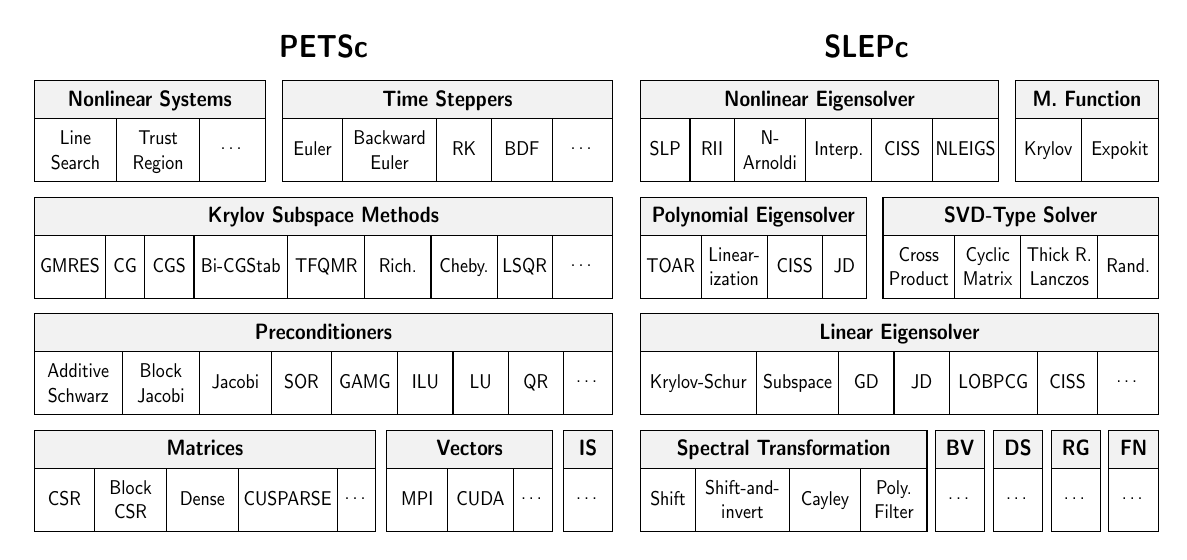
\begin{tikzpicture}[xscale=0.7,yscale=0.8]
  \tikzstyle{interface}=[fill=black!5,font=\sffamily\bfseries,text depth=.25ex]
  \tikzstyle{implem}=[font=\sffamily\small,text badly centered]
  \tikzstyle{every node}=[transform shape]
  \tikzstyle{onel}=[text depth=.25ex]
  \def\levsep{1.85} % separation of levels
  \def\hint{0.6} % height interface
  \def\himp{1} % height implementation
  \node[above,text centered,font=\sffamily\bfseries\Large] at (5.25,5*\levsep) {PETSc};
  \draw[interface] (0,\levsep+\himp) rectangle node {Matrices} +(6.2,\hint);
  \draw[implem] (0,\levsep) rectangle node[onel] {CSR} ++(1.1,1) ++(0,-1)
                rectangle node[text width=1.3cm] {Block CSR} ++(1.3,1) ++(0,-1)
                rectangle node[onel] {Dense} ++(1.3,1) ++(0,-1)
                rectangle node[onel] {CUSPARSE} ++(1.8,1) ++(0,-1)
                rectangle node[onel] {\dots} ++(.7,1);
  \draw[interface] (6.4,\levsep+\himp) rectangle node {Vectors} +(3,\hint);
  \draw[implem] (6.4,\levsep) rectangle node[onel] {MPI} ++(1.1,1) ++(0,-1)
                      rectangle node[onel] {CUDA} ++(1.2,1) ++(0,-1)
                      rectangle node[onel] {\dots} ++(.7,1);
  \draw[interface] (9.6,\levsep+\himp) rectangle node {IS} +(.9,\hint);
  \draw[implem] (9.6,\levsep) rectangle node[onel] {\dots} ++(.9,1);
  \draw[interface] (0,2*\levsep+\himp) rectangle node {Preconditioners} +(10.5,\hint);
  \draw[implem] (0,2*\levsep) rectangle node[text width=1.6cm] {Additive Schwarz} ++(1.6,1) ++(0,-1)
                rectangle node[text width=1.2cm] {Block Jacobi} ++(1.4,1) ++(0,-1)
                rectangle node[onel] {Jacobi} ++(1.3,1) ++(0,-1)
                rectangle node[onel] {SOR} ++(1.1,1) ++(0,-1)
                rectangle node[onel] {GAMG} ++(1.2,1) ++(0,-1)
                rectangle node[onel] {ILU} ++(1,1) ++(0,-1)
                rectangle node[onel] {LU} ++(1,1) ++(0,-1)
                rectangle node[onel] {QR} ++(1,1) ++(0,-1)
                rectangle node[onel] {\dots} ++(.9,1);
  \draw[interface] (0,3*\levsep+\himp) rectangle node {Krylov Subspace Methods} +(10.5,\hint);
  \draw[implem] (0,3*\levsep) rectangle node[onel] {GMRES} ++(1.3,1) ++(0,-1)
                rectangle node[onel] {CG} ++(0.7,1) ++(0,-1)
                rectangle node[onel] {CGS} ++(0.9,1) ++(0,-1)
                rectangle node[onel] {Bi-CGStab} ++(1.7,1) ++(0,-1)
                rectangle node[onel] {TFQMR} ++(1.4,1) ++(0,-1)
                rectangle node[onel] {Rich.} ++(1.2,1) ++(0,-1)
                rectangle node[onel] {Cheby.} ++(1.2,1) ++(0,-1)
                rectangle node[onel] {LSQR} ++(1,1) ++(0,-1)
                rectangle node[onel] {\dots} ++(1.1,1);
  \draw[interface] (0,4*\levsep+\himp) rectangle node {Nonlinear Systems} +(4.2,\hint);
  \draw[implem] (0,4*\levsep) rectangle node[text width=1.2cm] {Line Search} ++(1.5,1) ++(0,-1)
                rectangle node[text width=1.2cm,yshift=-1pt] {Trust Region} ++(1.5,1) ++(0,-1)
                rectangle node[onel] {\dots} ++(1.2,1);
  \draw[interface] (4.5,4*\levsep+\himp) rectangle node {Time Steppers} +(6,\hint);
  \draw[implem] (4.5,4*\levsep) rectangle node[onel] {Euler} ++(1.1,1) ++(0,-1)
                rectangle node[text width=1.5cm] {Backward Euler} ++(1.7,1) ++(0,-1)
                rectangle node[onel] {RK} ++(1.0,1) ++(0,-1)
                rectangle node[onel] {BDF} ++(1.1,1) ++(0,-1)
                rectangle node[onel] {\dots} ++(1.1,1);
  \node[above,text centered,font=\sffamily\bfseries\Large] at (15.1,5*\levsep) {SLEPc};
  \draw[interface] (11,4*\levsep+\himp) rectangle node {Nonlinear Eigensolver} +(6.5,\hint);
  \draw[implem] (11,4*\levsep) rectangle node[onel] {SLP} ++(.9,1) ++(0,-1)
                rectangle node[onel] {RII} ++(.8,1) ++(0,-1)
                rectangle node[text width=1.2cm] {N-Arnoldi} ++(1.3,1) ++(0,-1)
                rectangle node[onel] {Interp.} ++(1.2,1) ++(0,-1)
                rectangle node[onel] {CISS} ++(1.1,1) ++(0,-1)
                rectangle node[onel] {NLEIGS} ++(1.2,1);
  \draw[interface] (17.8,4*\levsep+\himp) rectangle node {M.~Function} +(2.6,\hint);
  \draw[implem] (17.8,4*\levsep) rectangle node[onel] {Krylov} ++(1.2,1) ++(0,-1)
                rectangle node[onel] {Expokit} ++(1.4,1);
  \draw[interface] (11,3*\levsep+\himp) rectangle node {Polynomial Eigensolver} +(4.1,\hint);
  \draw[implem] (11,3*\levsep) rectangle node[onel] {TOAR} ++(1.1,1) ++(0,-1)
                rectangle node[text width=1.2cm] {Linear\-ization} ++(1.2,1) ++(0,-1)
                rectangle node[onel] {CISS} ++(1,1) ++(0,-1)
                rectangle node[onel] {JD} ++(.8,1) ++(0,-1);
  \draw[interface] (15.4,3*\levsep+\himp) rectangle node {SVD-Type Solver} +(5,\hint);
  \draw[implem] (15.4,3*\levsep) rectangle node[text width=1.2cm] {Cross Product} ++(1.3,1) ++(0,-1)
                rectangle node[text width=1.2cm] {Cyclic Matrix} ++(1.2,1) ++(0,-1)
                rectangle node[text width=1.4cm] {Thick R. Lanczos} ++(1.4,1) ++(0,-1)
                rectangle node[onel] {Rand.} ++(1.1,1);
  \draw[interface] (11,2*\levsep+\himp) rectangle node {Linear Eigensolver} +(9.4,\hint);
  \draw[implem] (11,2*\levsep) rectangle node[onel] {Krylov-Schur} ++(2.1,1) ++(0,-1)
                rectangle node[onel] {Subspace} ++(1.5,1) ++(0,-1)
                rectangle node[onel] {GD} ++(1.0,1) ++(0,-1)
                rectangle node[onel] {JD} ++(1.0,1) ++(0,-1)
                rectangle node[onel] {LOBPCG} ++(1.6,1) ++(0,-1)
                rectangle node[onel] {CISS} ++(1.1,1) ++(0,-1)
                rectangle node[onel] {\dots} ++(1.1,1);
  \draw[interface] (11,\levsep+\himp) rectangle node {Spectral Transformation} +(5.2,\hint);
  \draw[implem] (11,\levsep) rectangle node[onel] {Shift} ++(1,1) ++(0,-1)
                rectangle node[text width=1.6cm] {Shift-and-invert} ++(1.7,1) ++(0,-1)
                rectangle node[onel] {Cayley} ++(1.3,1) ++(0,-1)
                rectangle node[text width=1.2cm] {Poly. Filter} ++(1.2,1);
  \draw[interface] (16.35,\levsep+\himp) rectangle node {BV} +(.9,\hint) ++(1.05,0)
                   rectangle node {DS} +(.9,\hint) ++(1.05,0)
                   rectangle node {RG} +(.9,\hint) ++(1.05,0)
                   rectangle node {FN} +(.9,\hint);
  \draw[implem] (16.35,\levsep) rectangle node[onel] {\dots} ++(.9,1);
  \draw[implem] (17.4,\levsep) rectangle node[onel] {\dots} ++(.9,1);
  \draw[implem] (18.45,\levsep) rectangle node[onel] {\dots} ++(.9,1);
  \draw[implem] (19.5,\levsep) rectangle node[onel] {\dots} ++(.9,1);
\end{tikzpicture}
\caption{\label{fig:slepc}Numerical components of \petsc and \slepc.}
\end{figure}

Each of these components consists of an abstract interface (simply a set of calling sequences) and one or more implementations using particular data structures. Both \petsc and \slepc are written in C, which lacks direct support for object-oriented programming. However, it is still possible to take advantage of the three basic principles of object-oriented programming to manage the complexity of such large packages. \petsc uses data \emph{encapsulation} in both vector and matrix data objects. Application code accesses data through function calls. Also, all the operations are supported through \emph{polymorphism}. The user calls a generic interface routine, which then selects the underlying routine that handles the particular data structure. Finally, \petsc also uses \emph{inheritance} in its design. All the objects are derived from an abstract base object. From this fundamental object, an abstract base object is defined for each \petsc\ object (\texttt{Mat}, \texttt{Vec} and so on), which in turn has a variety of instantiations that, for example, implement different matrix storage formats.

\petsc/\slepc provide clean and effective codes for the various phases of solving PDEs, with a uniform approach for each class of problems.  This design enables easy comparison and use of different algorithms (for example, to experiment with different Krylov subspace methods, preconditioners, or eigensolvers). Hence, \petsc, together with \slepc, provides a rich environment for modeling scientific applications as well as for rapid algorithm design and prototyping.

Options can be specified by means of calls to subroutines in the source code and also as command-line arguments. Runtime options allow the user to test different tolerances, for example, without having to recompile the program. Also, since \petsc provides a uniform interface to all of its linear solvers ---the Conjugate Gradient, GMRES, etc.--- and a large family of preconditioners ---block Jacobi, overlapping additive Schwarz, etc.---, one can compare several combinations of method and preconditioner by simply specifying them at execution time. \slepc shares this good property.

The components enable easy customization and extension of both algorithms and implementations. This approach promotes code reuse and flexibility, and separates the issues of parallelism from the choice of algorithms.  The \petsc infrastructure creates a foundation for building large-scale applications.

%---------------------------------------------------
\section{Installation}
\label{sec:inst}

This section describes \slepc's installation procedure.
Previously to the installation of \slepc, the system must have an appropriate version of \petsc\ installed. Compatible versions of \petsc and \slepc are those with coincident major and minor version number, the third number (patch level) being irrelevant for this. For instance, \slepc 3.23.x may be built with \petsc 3.23.x. Also note that, if using git repositories, both \petsc and \slepc must be either release versions or development versions, so make sure you select the appropriate branch in both repositories (\texttt{git checkout release} or \texttt{git checkout main}).

The installation process for \slepc is very similar to \petsc, with two stages: configuration and compilation. \slepc's configuration is much simpler because most of the configuration information is taken from \petsc, including compiler options and scalar type (real or complex). See \S\ref{sec:opt-inst} for a discussion of options that are most relevant for \slepc. Several configurations can coexist in the same directory tree, so that for instance one can have \slepc libraries compiled with real scalars as well as with complex scalars. This is explained in \S\ref{sec:mult-inst}. Also, system-based installation is also possible with the \Verb!--prefix! option, as discussed in \S\ref{sec:prefix-inst}.

\subsection{Standard Installation}
\label{sec:std-inst}

The basic steps for the installation are described next. Note that prior to these steps, optional packages must have been installed. If any of these packages is installed afterwards, reconfiguration and recompilation is necessary. Refer to \S\ref{sec:opt-inst} and \S\ref{sec:wrap} for details about installation of some of these packages.

\begin{enumerate}
\item Unbundle the distribution file with
        \begin{Verbatim}[fontsize=\small]
        $ tar xzf slepc-3.23.0.tar.gz
        \end{Verbatim}
        or an equivalent command. This will create a directory and unpack the software there.
\item Set the environment variable \ident{SLEPC\_DIR} to the full path of the \slepc home directory. For example, under the \texttt{bash} shell:
        \begin{Verbatim}[fontsize=\small]
        $ export SLEPC_DIR=/home/username/slepc-3.23.0
        \end{Verbatim}
In addition, the variables \ident{PETSC\_DIR} and \ident{PETSC\_ARCH} must also be set appropriately, e.g.
        \begin{Verbatim}[fontsize=\small]
        $ export PETSC_DIR=/home/username/petsc-3.23.0
        $ export PETSC_ARCH=arch-darwin-c-debug
        \end{Verbatim}
        The rationale for \ident{PETSC\_ARCH} is explained in \S\ref{sec:mult-inst} (see \S\ref{sec:prefix-inst} for a case in which \ident{PETSC\_ARCH} is not required).
\item\label{step-config} Change to the \slepc directory and run the configuration script:
        \begin{Verbatim}[fontsize=\small]
        $ cd $SLEPC_DIR
        $ ./configure
        \end{Verbatim}
\item If the configuration was successful, build the libraries:
        \begin{Verbatim}[fontsize=\small]
        $ make
        \end{Verbatim}
\item After the compilation, try running some test examples with
        \begin{Verbatim}[fontsize=\small]
        $ make check
        \end{Verbatim}
        Examine the output for any obvious errors or problems.
\end{enumerate}

\subsection{Configuration Options}
\label{sec:opt-inst}

Several options are available in \slepc's configuration script. To see all available options, type \Verb!./configure --help!.

In \slepc, configure options have the following purposes:
\begin{itemize}
%\item Build \slepc with Python interfaces, as explained in \S\ref{sec:py-inst}.
\item Specify a directory for prefix-based installation, as explained in \S\ref{sec:prefix-inst}.
\item Enable external eigensolver packages. For example, to use \arpack, specify the following options (with the appropriate paths):
        \begin{Verbatim}[fontsize=\small]
        $ ./configure --with-arpack-dir=/usr/software/ARPACK
        \end{Verbatim}
Some of the external packages also support the \Verb!--download-xxxx! option. Section \ref{sec:wrap} provides more details related to use of external libraries.
\end{itemize}

Additionally, \petsc's configuration script provides a very long list of options that are relevant to \slepc. Here is a list of options that may be useful. Note that these are options of \petsc that apply to both \petsc and \slepc, in such a way that it is not possible to, e.g., build \petsc without debugging and \slepc with debugging.
\begin{itemize}
\item Add \Verb!--with-scalar-type=complex! to build complex scalar versions of all libraries. See below a note related to complex scalars.
\item Build single precision versions with \Verb!--with-precision=single!. In most applications, this can achieve a significant reduction of memory requirements, and a moderate reduction of computing time. Also, quadruple precision (128-bit floating-point representation) is also available using \Verb!--with-precision=__float128! on systems with GNU compilers (\texttt{gcc-4.6} or later).
\item Enable use from Fortran. By default, \petsc's configure looks for an appropriate Fortran compiler. If not required, this can be disabled: \Verb!--with-fc=0!. If required but not correctly detected, the compiler to be used can be specified with a configure option. It is also possible to configure with a Fortran compiler but do not build Fortran interfaces of \petsc and \slepc, with \Verb!--with-fortran-bindings=0!.
\item If not detected, use \Verb!--with-blas-lapack-lib! to specify the location of \blas and \lapack. If \slepc's configure complains about some missing \lapack subroutines, reconfigure \petsc with option \Verb!--download-f2cblaslapack!.
\item Enable external libraries that provide direct linear solvers or preconditioners, such as MUMPS, hypre, or SuperLU; for example, \Verb!--download-mumps!. These are especially relevant for \slepc in the case that a spectral transformation is used, see chapter \ref{cap:st}.
\item Add \Verb!--with-64-bit-indices=1! to use 8 byte integers (\texttt{long long}) for indexing in vectors and matrices. This is only needed when working with over roughly 2 billion unknowns.
\item Build static libraries, \Verb!--with-shared-libraries=0!. This is generally not recommended, since shared libraries produce smaller executables and the run time overhead is small.
\item Error-checking code can be disabled with \Verb!--with-debugging=0!, but this is only recommended in production runs of well-tested applications.
\item Enable GPU computing setting \Verb!--with-cuda=1! or \Verb!--with-hip=1!; see \S\ref{sec:gpu} for details.
\item The option \Verb!--with-mpi=0! allows building \petsc and \slepc without MPI support (only sequential).
\end{itemize}

\medskip
\textbf{Note about complex scalar versions}: \petsc supports the use of complex scalars by defining the data type \ident{PetscScalar} either as a real or complex number. This implies that two different versions of the \petsc libraries can be built separately, one for real numbers and one for complex numbers, but they cannot be used at the same time. \slepc inherits this property. In \slepc it is not possible to completely separate real numbers and complex numbers because the solution of non-symmetric real-valued eigenvalue problems may be complex. \slepc has been designed trying to provide a uniform interface to manage all the possible cases. However, there are slight differences between the interface in each of the two versions. In this manual, differences are clearly identified.

\subsection{Installing Multiple Configurations in a Single Directory Tree}
\label{sec:mult-inst}

Often, it is necessary to build two (or more) versions of the libraries that differ in a few configuration options. For instance, versions for real and complex scalars, or versions for double and single precision, or versions with debugging and optimized. In a standard installation, this is handled by building all versions in the same directory tree, as explained below, so that source code is not replicated unnecessarily. In contrast, in prefix-based installation where source code is not present, the issue of multiple configurations is handled differently, as explained in \S\ref{sec:prefix-inst}.

In a standard installation, the different configurations are identified by a unique name that is assigned to the environment variable \ident{PETSC\_ARCH}. Let us illustrate how to set up \petsc with two configurations. First, set a value of \ident{PETSC\_ARCH} and proceed with the installation of the first one:
        \begin{Verbatim}[fontsize=\small]
        $ cd $PETSC_DIR
        $ export PETSC_ARCH=arch-linux-gnu-c-debug-real
        $ ./configure --with-scalar-type=real
        $ make all
        \end{Verbatim}
Note that if \ident{PETSC\_ARCH} is not given a value, \petsc suggests one for us. After this, a subdirectory named \texttt{\$PETSC\_ARCH} is created within \texttt{\$PETSC\_DIR}, that stores all information associated with that configuration, including the built libraries, configuration files, automatically generated source files, and log files. For the second configuration, proceed similarly:
        \begin{Verbatim}[fontsize=\small]
        $ cd $PETSC_DIR
        $ export PETSC_ARCH=arch-linux-gnu-c-debug-complex
        $ ./configure --with-scalar-type=complex
        $ make all
        \end{Verbatim}
The value of \ident{PETSC\_ARCH} in this case must be different than the previous one. It is better to set the value of \ident{PETSC\_ARCH} explicitly, because the name suggested by \texttt{configure} may coincide with an existing value, thus overwriting a previous configuration. After successful installation of the second configuration, two \texttt{\$PETSC\_ARCH} directories exist within \texttt{\$PETSC\_DIR}, and the user can easily choose to build his/her application with either configuration by simply changing the value of \ident{PETSC\_ARCH}.

The configuration of two versions of \slepc in the same directory tree is very similar. The only important restriction is that the value of \ident{PETSC\_ARCH} used in \slepc must exactly match an existing \petsc configuration, that is, a directory \texttt{\$PETSC\_DIR/\$PETSC\_ARCH} must exist.

\subsection{Prefix-based Installation}
\label{sec:prefix-inst}

Both \petsc and \slepc allow for prefix-based installation. This consists in specifying a directory to which the files generated during the building process are to be copied.

In \petsc, if an installation directory has been specified during configuration (with option \Verb!--prefix! in step \ref{step-config} of \S\ref{sec:std-inst}), then after building the libraries the relevant files are copied to that directory by typing
        \begin{Verbatim}[fontsize=\small]
        $ make install
        \end{Verbatim}
This is useful for building as a regular user and then copying the libraries and include files to the system directories as root.

To be more precise, suppose that the configuration was done with \texttt{-{}-prefix=/opt/petsc-3.23.0-linux-gnu-c-debug}. Then, \texttt{make install} will create directory \texttt{/opt/petsc-3.23.0-linux-gnu-c-debug} if it does not exist, and several subdirectories containing the libraries, the configuration files, and the header files. Note that the source code files are not copied, nor the documentation, so the size of the installed directory will be much smaller than the original one. For that reason, it is no longer necessary to allow for several configurations to share a directory tree. In other words, in a prefix-based installation, variable \ident{PETSC\_ARCH} loses significance and must be unset. To maintain several configurations, one should specify different prefix directories, typically with a name that informs about the configuration options used.

In order to prepare a prefix-based installation of \slepc that uses a prefix-based installation of \petsc, start by setting the appropriate value of \ident{PETSC\_DIR}. Then, run \slepc's configure with a prefix directory.
        \begin{Verbatim}[fontsize=\small,numbers=none]
        $ export PETSC_DIR=/opt/petsc-3.23.0-linux-gnu-c-debug
        $ unset PETSC_ARCH
        $ cd $SLEPC_DIR
        $ ./configure --prefix=/opt/slepc-3.23.0-linux-gnu-c-debug
        $ make
        $ make install
        $ export SLEPC_DIR=/opt/slepc-3.23.0-linux-gnu-c-debug
        \end{Verbatim}
Note that the variable \ident{PETSC\_ARCH} has been unset before \slepc's configure. \slepc will use a temporary arch name during the build (this temporary arch is named \texttt{installed-arch-xxx}, where the \texttt{arch-xxx} string represents the configuration of the installed \petsc version). Although it is not a common case, it is also possible to configure \slepc without prefix, in which case the \ident{PETSC\_ARCH} variable must still be empty and the arch directory \texttt{installed-xxx} is picked automatically (it is hardwired in file \texttt{\$SLEPC\_DIR/lib/slepc/conf/slepcvariables}). The combination \petsc without prefix and \slepc with prefix is also allowed, in which case \ident{PETSC\_ARCH} should not be unset.

%\subsection{Building Python Interfaces}
%\label{sec:py-inst}

%---------------------------------------------------
\section{Running SLEPc Programs}

Before using \slepc, the user must first set the environment variable
\ident{SLEPC\_DIR}, indicating the full path of the directory containing \slepc. For example, under the \texttt{bash} shell, a command of the form
        \begin{Verbatim}[fontsize=\small]
        $ export SLEPC_DIR=/software/slepc-3.23.0
        \end{Verbatim}
can be placed in the user's \Verb!.bashrc! file.
The \ident{SLEPC\_DIR} directory can be either a standard installation \slepc directory, or a prefix-based installation directory, see \S\ref{sec:prefix-inst}.
In addition, the user must set the environment variables required by \petsc, that is, \ident{PETSC\_DIR}, to indicate the full path of the \petsc directory, and \ident{PETSC\_ARCH} to specify a particular architecture and set of options. Note that \ident{PETSC\_ARCH} should not be set in the case of prefix-based installations.

All \petsc programs use the MPI (Message Passing Interface) standard
for message-passing communication \citep{MPI-Forum:1994:MMI}.  Thus, to execute
\slepc programs, users must know the procedure for launching MPI jobs
on their selected computer system(s).  Usually, the \texttt{mpiexec} command can be used to initiate a program as in the following example that uses eight processes:
        \begin{Verbatim}[fontsize=\small]
        $ mpiexec -n 8 slepc_program [command-line options]
        \end{Verbatim}
Note that MPI may be deactivated during configuration of \petsc, if one wants to run only serial programs in a laptop, for example.

All \petsc-compliant programs support the use of the \Verb!-h!
or \Verb!-help! option as well as the \Verb!-v! or \Verb!-version! option. In the case of \slepc programs, specific information for \slepc is also displayed.

%---------------------------------------------------
\section{Writing SLEPc Programs}

Most \slepc programs begin with a call to \rutina{SlepcInitialize}
        \begin{Verbatim}[fontsize=\small]
        SlepcInitialize(int *argc,char ***argv,char *file,char *help);
        \end{Verbatim}
which initializes \slepc, \petsc and MPI. This subroutine is very similar to \rutina{PetscInitialize}, and the arguments have the same meaning. In fact, internally \rutina{SlepcInitialize} calls \rutina{PetscInitialize}.

After this initialization, \slepc programs can use communicators defined by \petsc. In most cases users can employ the communicator \ident{PETSC\_COMM\_WORLD} to indicate all processes in a given run and \ident{PETSC\_COMM\_SELF} to indicate a single process. MPI provides routines for generating new communicators consisting of subsets of processes, though most users rarely need to use these features. \slepc users need not program much message passing directly with MPI, but they must be familiar with the basic concepts of message passing and distributed memory computing.

All \slepc programs should call \rutina{SlepcFinalize} as their final (or nearly final) statement
        \begin{Verbatim}[fontsize=\small]
        SlepcFinalize();
        \end{Verbatim}
This routine handles operations to be executed at the conclusion of the program, and calls \rutina{PetscFinalize} if \rutina{SlepcInitialize} began \petsc.

\medskip
\textbf{Note to Fortran Programmers}: In this manual all the examples and calling sequences are given for the C/C++ programming languages. However, Fortran programmers can use most of the functionality of \slepc and \petsc from Fortran, with only minor differences in the user interface. For instance, the two functions mentioned above have their corresponding Fortran equivalent:
        \begin{Verbatim}[fontsize=\small]
        call SlepcInitialize(file,ierr)
        call SlepcFinalize(ierr)
        \end{Verbatim}
Section \ref{sec:fortran} provides a summary of the differences between using \slepc from Fortran and C/C++, as well as a complete Fortran example.

%---------------------------------------------------
\subsection{Simple SLEPc Example}
\label{sec:simpleex}

A simple example is listed next that solves an eigenvalue problem associated with the one-dimensional Laplacian operator discretized with finite differences. This example can be found in \Verb!${SLEPC_DIR}/src/eps/tutorials/ex1.c!. Following the code we highlight a few of the most important parts of this example.

\MyVerbatimInput{ex1.c}

\paragraph{Include Files.}

The C/C++ include files for \slepc should be used via statements such as
        \begin{Verbatim}[fontsize=\small]
        #include <slepceps.h>
        \end{Verbatim}
where \Verb!slepceps.h! is the include file for the \ident{EPS} component. Each \slepc program must specify an include file that corresponds to the highest level \slepc objects needed within the program; all of the required lower level include files are automatically included within the higher level files. For example, \Verb!slepceps.h! includes \Verb!slepcst.h! (spectral transformations), and \Verb!slepcsys.h! (base \slepc file). Some \petsc header files are included as well, such as \Verb!petscksp.h!. The \slepc include files are located in the directory \Verb!${SLEPC_DIR}/include!.

\paragraph{The Options Database.}

All the \petsc functionality related to the options database is available in \slepc. This allows the user to input control data at run time very easily. In this example, the call \Verb!PetscOptionsGetInt(NULL,NULL,"-n",&n,NULL)! checks whether the user has provided a command line option to set the value of \Verb!n!, the problem dimension.  If so, the variable \Verb!n! is set accordingly; otherwise, \Verb!n! remains unchanged.

\paragraph{Vectors and Matrices.}

Usage of matrices and vectors in \slepc is exactly the same as in \petsc. The user can create a new parallel or sequential matrix, \texttt{A}, which has \texttt{M} global rows and \texttt{N} global columns, with
        \begin{Verbatim}[fontsize=\small]
        MatCreate(MPI_Comm comm,Mat *A);
        MatSetSizes(Mat A,PetscInt m,PetscInt n,PetscInt M,PetscInt N);
        MatSetFromOptions(Mat A);
        \end{Verbatim}
where the matrix format can be specified at runtime. The example creates a matrix, sets the nonzero values with \rutina{MatSetValues} and then assembles it.

\paragraph{Eigensolvers.}

Usage of eigensolvers is very similar to other kinds of solvers provided by \petsc. After creating the matrix (or matrices) that define the problem, $Ax = kx$ (or $Ax=kBx$), the user can then use \ident{EPS} to solve the system with the following sequence of commands:
\findex{EPSCreate} \findex{EPSSetOperators} \findex{EPSSetProblemType}
\findex{EPSSetFromOptions} \findex{EPSSolve} \findex{EPSDestroy}
\findex{EPSGetConverged} \findex{EPSGetEigenpair}
        \begin{Verbatim}[fontsize=\small,numbers=none]
        EPSCreate(MPI_Comm comm,EPS *eps);
        EPSSetOperators(EPS eps,Mat A,Mat B);
        EPSSetProblemType(EPS eps,EPSProblemType type);
        EPSSetFromOptions(EPS eps);
        EPSSolve(EPS eps);
        EPSGetConverged(EPS eps,PetscInt *nconv);
        EPSGetEigenpair(EPS eps,PetscInt i,PetscScalar *kr,PetscScalar *ki,Vec xr,Vec xi);
        EPSDestroy(EPS *eps);
        \end{Verbatim}
The user first creates the \ident{EPS} context and sets the operators associated with the eigensystem as well as the problem type. The user then sets various options for customized solution, solves the problem, retrieves the solution, and finally destroys the \ident{EPS} context. Chapter~\ref{cap:eps} describes in detail the \ident{EPS} package, including
the options database that enables the user to customize the solution process at runtime by selecting the solution algorithm and also specifying the convergence tolerance, the number of eigenvalues, the dimension of the subspace, etc.

\paragraph{Spectral Transformation.}

In the example program shown above there is no explicit reference to spectral transformations. However, an \ident{ST} object is handled internally so that the user is able to request different transformations such as shift-and-invert. Chapter~\ref{cap:st} describes the \ident{ST} package in detail.

\paragraph{Error Checking.}

All \slepc routines return an integer indicating whether an error has occurred during the call. The error code is set to be nonzero if an error has been detected; otherwise, it is zero. The \petsc macro \Verb!PetscCall(...)! checks the return value and calls the \petsc error handler upon error detection. \Verb!PetscCall(...)! should be used in all subroutine calls to enable a complete error traceback. See the \petsc documentation for full details.

\subsection{Writing Application Codes with SLEPc}

Several example programs demonstrate the software usage and can serve as templates for developing custom applications. They are scattered throughout the \slepc directory tree, in particular in the \Verb!tutorials! directories under each class subdirectory.

To write a new application program using \slepc, we suggest the following procedure:
\begin{enumerate}
\item Install and test \slepc according to the instructions given in the documentation.
\item Copy the \slepc example that corresponds to the class of problem of interest (e.g., singular value decomposition).
\item Create a makefile as explained below, compile and run the example program.
\item Use the example program as a starting point for developing a custom code.
\end{enumerate}

Application program makefiles can be set up very easily just by including one file from the \slepc makefile system. All the necessary \petsc{} definitions are loaded automatically. The following sample makefile illustrates how to build C and Fortran programs:

\begin{Verbatim}[fontsize=\small]
default: ex1

include ${SLEPC_DIR}/lib/slepc/conf/slepc_common

ex1: ex1.o
        -${CLINKER} -o ex1 ex1.o ${SLEPC_EPS_LIB}
        ${RM} ex1.o

ex1f: ex1f.o
        -${FLINKER} -o ex1f ex1f.o ${SLEPC_EPS_LIB}
        ${RM} ex1f.o
\end{Verbatim}


%-------------------------------------------------------
% SLEPc Users Manual
%-------------------------------------------------------
\chapter{\label{cap:eps}EPS: Eigenvalue Problem Solver}
%-------------------------------------------------------

\noindent The Eigenvalue Problem Solver (\ident{EPS}) is the main object provided by \slepc. It is used to specify a linear eigenvalue problem, either in standard or generalized form, and provides uniform and efficient access to all of the linear eigensolvers included in the package. Conceptually, the level of abstraction occupied by \ident{EPS} is similar to other solvers in \petsc\ such as \ident{KSP} for solving linear systems of equations.

\section{\label{sec:eig}Eigenvalue Problems}

In this section, we briefly present some basic concepts about eigenvalue problems as well as general techniques used to solve them. The description is not intended to be exhaustive. The objective is simply to define terms that will be referred to throughout the rest of the manual. Readers who are familiar with the terminology and the solution approach can skip this section. For a more comprehensive description, we refer the reader to monographs such as \citep{Stewart:2001:MAV}, \citep{Bai:2000:TSA}, \citep{Saad:1992:NML} or \citep{Parlett:1980:SEP}. A historical perspective of the topic can be found in \citep{Golub:2000:EC2}. See also the \slepc \hyperlink{str}{technical reports}.

In the standard formulation, the linear eigenvalue problem consists in the determination of $\lambda\in\mathbb{C}$ for which the equation
\begin{equation}
Ax=\lambda x\label{eq:eigstd}
\end{equation}
has nontrivial solution, where $A\in\mathbb{C}^{n\times n}$ and $x\in\mathbb{C}^n$. The scalar $\lambda$ and the vector $x$ are called eigenvalue and (right) eigenvector, respectively. Note that they can be complex even when the matrix is real. If $\lambda$ is an eigenvalue of $A$ then $\bar{\lambda}$ is an eigenvalue of its conjugate transpose, $A^*$, or equivalently
\begin{equation}
y^*\!A=\lambda\, y^*,\label{eq:eigstdleft}
\end{equation}
where $y$ is called the left eigenvector.

In many applications, the problem is formulated as
\begin{equation}
Ax=\lambda Bx,\label{eq:eiggen}
\end{equation}
where $B\in\mathbb{C}^{n\times n}$, which is known as the generalized eigenvalue problem. Usually, this problem is solved by reformulating it in standard form, for example $B^{-1}Ax=\lambda x$ if $B$ is non-singular.

\slepc focuses on the solution of problems in which the matrices are large and sparse. Hence, only methods that preserve sparsity are considered.
These methods obtain the solution from the information generated by the application of the operator to various vectors (the operator is a simple function of matrices $A$ and $B$), that is, matrices are only used in matrix-vector products. This not only maintains sparsity but allows the solution of problems in which matrices are not available explicitly.

In practical analyses, from the $n$ possible solutions, typically only a few eigenpairs $(\lambda,x)$ are considered relevant, either in the extremities of the spectrum, in an interval, or in a region of the complex plane.
Depending on the application, either eigenvalues or eigenvectors (or both) are required. In some cases, left eigenvectors are also of interest.

\paragraph{Projection Methods.}

Most eigensolvers provided by \slepc perform a Rayleigh-Ritz projection for extracting the spectral approximations, that is, they project the problem onto a low-dimensional subspace that is built appropriately. Suppose that an orthogonal basis of this subspace is given by $V_j=[v_1,v_2,\ldots,v_j]$. If the solutions of the projected (reduced) problem $B_js=\theta s$ (i.e., $V_j^TAV_j=B_j$) are assumed to be $(\theta_i,s_i)$, $i=1,2,\ldots,j$, then the approximate eigenpairs $(\tilde{\lambda}_i,\tilde{x}_i)$ of the original problem (Ritz value and Ritz vector) are obtained as
\begin{eqnarray}
\tilde{\lambda}_i=\theta_i,\\
\tilde{x}_i=V_js_i.
\end{eqnarray}
Starting from this general idea, eigensolvers differ from each other in which subspace is used, how it is built and other technicalities aimed at improving convergence, reducing storage requirements, etc.

The subspace
\begin{equation}
\mathcal{K}_m(A,v)\equiv\mathrm{span}\left\{v,Av,A^2v,\ldots,A^{m-1}v\right\},\label{eq:krylov}
\end{equation}
is called the $m$-th Krylov subspace corresponding to $A$ and $v$. Methods that use subspaces of this kind to carry out the projection are called Krylov methods. One example of such methods is the Arnoldi algorithm: starting with $v_1$, $\|v_1\|_2=1$, the Arnoldi basis generation process can be expressed by the recurrence
\begin{equation}
v_{j+1}h_{j+1,j}=w_j=Av_j-\sum_{i=1}^jh_{i,j}v_i,
\end{equation}
where $h_{i,j}$ are the scalar coefficients obtained in the Gram-Schmidt orthogonalization of $Av_j$ with respect to $v_i$, $i=1,2,\ldots,j$, and $h_{j+1,j}=\|w_j\|_2$. Then, the columns of $V_j$ span the Krylov subspace $\mathcal{K}_j(A,v_1)$ and $Ax=\lambda x$ is projected into $H_js=\theta s$, where $H_j$ is an upper Hessenberg matrix with elements $h_{i,j}$, which are 0 for $i\geq j+2$. The related Lanczos algorithms obtain a projected matrix that is tridiagonal.

A generalization to the above methods are the block Krylov strategies, in which the starting vector $v_1$ is replaced by a full rank $n\times p$ matrix $V_1$, which allows for better convergence properties when there are multiple eigenvalues and can provide better data management on some computer architectures. Block tridiagonal and block Hessenberg matrices are then obtained as projections.

It is generally assumed (and observed) that the Lanczos and Arnoldi algorithms find solutions at the extremities of the spectrum. Their convergence pattern, however, is strongly related to the eigenvalue distribution. Slow convergence may be experienced in the presence of tightly clustered eigenvalues. The maximum allowable $j$ may be reached without having achieved convergence for all desired solutions. Then, restarting is usually a useful technique and different strategies exist for that purpose. However, convergence can still be very slow and acceleration strategies must be applied. Usually, these techniques consist in computing eigenpairs of a transformed operator and then recovering the solution of the original problem. The aim of these transformations is twofold. On one hand, they make it possible to obtain eigenvalues other than those lying in the periphery of the spectrum. On the other hand, the separation of the eigenvalues of interest is improved in the transformed spectrum thus leading to faster convergence. The most commonly used spectral transformation is called shift-and-invert, which works with operator $(A-\sigma I)^{-1}$. It allows the computation of eigenvalues closest to $\sigma$ with very good separation properties. When using this approach, a linear system of equations, $(A-\sigma I)y=x$, must be solved in each iteration of the eigenvalue process.

\paragraph{Preconditioned Eigensolvers.}
In many applications, Krylov eigensolvers perform very well because Krylov subspaces are optimal in a certain theoretical sense. However, these methods may not be appropriate in some situations such as the computation of interior eigenvalues. The spectral transformation mentioned above may not be a viable solution or it may be too costly. For these reasons, other types of eigensolvers such as Davidson and Jacobi-Davidson rely on a different way of expanding the subspace. Instead of satisfying the Krylov relation, these methods compute the new basis vector by the so-called correction equation. The resulting subspace may be richer in the direction of the desired eigenvectors. These solvers may be competitive especially for computing interior eigenvalues. From a practical point of view, the correction equation may be seen as a cheap replacement for the shift-and-invert system of equations, $(A-\sigma I)y=x$. By cheap we mean that it may be solved inaccurately without compromising robustness, via a preconditioned iterative linear solver. For this reason, these are known as \emph{preconditioned} eigensolvers.

\paragraph{Related Problems.}

In many applications such as the analysis of damped vibrating systems the problem to be solved is a \emph{polynomial eigenvalue problem} (PEP), or more generally a \emph{nonlinear eigenvalue problem} (NEP). For these, the reader is referred to chapters \ref{cap:pep} and \ref{cap:nep}. Another linear algebra problem that is very closely related to the eigenvalue problem is the {\em singular value decomposition\/} (SVD), see chapter \ref{cap:svd}.

%---------------------------------------------------
\section{Basic Usage}

The \ident{EPS} module in \slepc is used in a similar way as \petsc modules such as \ident{KSP}. All the information related to an eigenvalue problem is handled via a context variable. The usual object management functions are available (\ident{EPSCreate}, \ident{EPSDestroy}, \ident{EPSView}, \ident{EPSSetFromOptions}). In addition, the \ident{EPS} object provides functions for setting several parameters such as the number of eigenvalues to compute, the dimension of the subspace, the portion of the spectrum of interest, the requested tolerance or the maximum number of iterations allowed.

The solution of the problem is obtained in several steps. First of all, the matrices associated with the eigenproblem are specified via \ident{EPSSetOperators} and \ident{EPSSetProblemType} is used to specify the type of problem. Then, a call to \ident{EPSSolve} is done that invokes the subroutine for the selected eigensolver. \ident{EPSGetConverged} can be used afterwards to determine how many of the requested eigenpairs have converged to working accuracy. \ident{EPSGetEigenpair} is finally used to retrieve the eigenvalues and eigenvectors.

In order to illustrate the basic functionality of the \ident{EPS} package, a simple example is shown in Figure \ref{fig:ex-eps}. The example code implements the solution of a simple standard eigenvalue problem. Code for setting up the matrix $A$ is not shown and error-checking code is omitted.

\begin{figure}
\begin{Verbatim}[fontsize=\small,numbers=left,numbersep=6pt,xleftmargin=15mm]
EPS         eps;       /*  eigensolver context  */
Mat         A;         /*  matrix of Ax=kx      */
Vec         xr, xi;    /*  eigenvector, x       */
PetscScalar kr, ki;    /*  eigenvalue, k        */
PetscInt    j, nconv;
PetscReal   error;

EPSCreate( PETSC_COMM_WORLD, &eps );
EPSSetOperators( eps, A, NULL );
EPSSetProblemType( eps, EPS_NHEP );
EPSSetFromOptions( eps );
EPSSolve( eps );
EPSGetConverged( eps, &nconv );
for (j=0; j<nconv; j++) {
  EPSGetEigenpair( eps, j, &kr, &ki, xr, xi );
  EPSComputeError( eps, j, EPS_ERROR_RELATIVE, &error );
}
EPSDestroy( &eps );
\end{Verbatim}
\caption{\label{fig:ex-eps}Example code for basic solution with \ident{EPS}.}
\end{figure}

All the operations of the program are done over a single \ident{EPS} object. This solver context is created in line 8 with the command
        \findex{EPSCreate}
        \begin{Verbatim}[fontsize=\small]
        EPSCreate(MPI_Comm comm,EPS *eps);
        \end{Verbatim}
Here \texttt{comm} is the MPI communicator, and \texttt{eps} is the newly formed solver context. The communicator indicates which processes are involved in the \ident{EPS} object. Most of the \ident{EPS} operations are collective, meaning that all the processes collaborate to perform the operation in parallel.

Before actually solving an eigenvalue problem with \ident{EPS}, the user must specify the matrices associated with the problem, as in line 9, with the following routine
        \findex{EPSSetOperators}
        \begin{Verbatim}[fontsize=\small]
        EPSSetOperators(EPS eps,Mat A,Mat B);
        \end{Verbatim}
The example specifies a standard eigenproblem. In the case of a generalized problem, it would be necessary also to provide matrix $B$ as the third argument to the call. The matrices specified in this call can be in any \petsc format. In particular, \ident{EPS} allows the user to solve matrix-free problems by specifying matrices created via \ident{MatCreateShell}. A more detailed discussion of this issue is given in \S\ref{sec:supported}.

After setting the problem matrices, the problem type is set with \ident{EPSSetProblemType}. This is not strictly necessary since if this step is skipped then the problem type is assumed to be non-symmetric. More details are given in \S\ref{sec:defprob}.
At this point, the value of the different options could optionally be set by means of a function call such as \ident{EPSSetTolerances} (explained later in this chapter). After this, a call to \ident{EPSSetFromOptions} should be made as in line 11,
        \findex{EPSSetFromOptions}
        \begin{Verbatim}[fontsize=\small]
        EPSSetFromOptions(EPS eps);
        \end{Verbatim}
The effect of this call is that options specified at runtime in the command line are passed to the \ident{EPS} object appropriately. In this way, the user can easily experiment with different combinations of options without having to recompile. All the available options as well as the associated function calls are described later in this chapter.

Line 12 launches the solution algorithm, simply with the command
        \findex{EPSSolve}
        \begin{Verbatim}[fontsize=\small]
        EPSSolve(EPS eps);
        \end{Verbatim}
The subroutine that is actually invoked depends on which solver has been selected by the user.

        After the call to \ident{EPSSolve} has finished, all the data associated with the solution of the eigenproblem are kept internally. This information can be retrieved with different function calls, as in lines 13 to 17. This part is described in detail in \S\ref{sec:retrsol}.

Once the \ident{EPS} context is no longer needed, it should be destroyed with the command
        \findex{EPSDestroy}
        \begin{Verbatim}[fontsize=\small]
        EPSDestroy(EPS *eps);
        \end{Verbatim}

The above procedure is sufficient for general use of the \ident{EPS} package. As in the case of the \ident{KSP} solver, the user can optionally explicitly call
        \findex{EPSSetUp}
        \begin{Verbatim}[fontsize=\small]
        EPSSetUp(EPS eps);
        \end{Verbatim}
before calling \ident{EPSSolve} to perform any setup required for the eigensolver.

Internally, the \ident{EPS} object works with an \ident{ST} object (spectral transformation, described in chapter \ref{cap:st}). To allow application programmers to set any of the spectral transformation options directly within the code, the following routine is provided to extract the \ident{ST} context,
        \findex{EPSGetST}
        \begin{Verbatim}[fontsize=\small]
        EPSGetST(EPS eps,ST *st);
        \end{Verbatim}

With the command
        \findex{EPSView}
        \begin{Verbatim}[fontsize=\small]
        EPSView(EPS eps,PetscViewer viewer);
        \end{Verbatim}
it is possible to examine the actual values of the different settings of the \ident{EPS} object, including also those related to the associated \ident{ST} object. This is useful for making sure that the solver is using the settings that the user wants.

%---------------------------------------------------
\section{Defining the Problem}
\label{sec:defprob}

\slepc is able to cope with different kinds of problems. Currently supported problem types are listed in Table \ref{tab:ptype}. An eigenproblem is generalized ($Ax=\lambda Bx$) if the user has specified two matrices (see \ident{EPSSetOperators} above), otherwise it is standard ($Ax=\lambda x$). A standard eigenproblem is Hermitian if matrix $A$ is Hermitian (i.e., $A=A^*$) or, equivalently in the case of real matrices, if matrix $A$ is symmetric (i.e., $A=A^T$). A generalized eigenproblem is Hermitian if matrix $A$ is Hermitian (symmetric) and $B$ is Hermitian (symmetric) and positive (semi-)definite.
If $B$ is not positive (semi-)definite then the problem cannot be considered Hermitian but symmetry can still be exploited to some extent in some solvers (problem type \texttt{EPS\_GHIEP}).
A special case of generalized non-Hermitian problem is when $A$ is non-Hermitian but $B$ is Hermitian and positive (semi-)definite, see \S\ref{sec:symm} and \S\ref{sec:purif} for discussion.
The last entries in Table \ref{tab:ptype}, separated by a line, correspond to structured eigenvalue problems, which are discussed in \S\ref{sec:structured}.

\begin{table}[t]
\centering
{\small \begin{tabular}{lll}
Problem Type              & \ident{EPSProblemType}    & Command line key\\\hline
Hermitian                 & \texttt{EPS\_HEP}         & \texttt{-eps\_hermitian}\\
Non-Hermitian             & \texttt{EPS\_NHEP}        & \texttt{-eps\_non\_hermitian}\\
Generalized Hermitian     & \texttt{EPS\_GHEP}        & \texttt{-eps\_gen\_hermitian}\\
Generalized Hermitian indefinite & \texttt{EPS\_GHIEP} & \texttt{-eps\_gen\_indefinite}\\
Generalized Non-Hermitian & \texttt{EPS\_GNHEP}       & \texttt{-eps\_gen\_non\_hermitian}\\
GNHEP with positive (semi-)definite $B$ & \texttt{EPS\_PGNHEP} & \texttt{-eps\_pos\_gen\_non\_hermitian}\\\hline
Bethe-Salpeter            & \texttt{EPS\_BSE}         & \texttt{-eps\_bse}\\\hline
\end{tabular} }
\caption{\label{tab:ptype}Problem types considered in \ident{EPS}.}
\end{table}

The problem type can be specified at run time with the corresponding command line key or, more usually, within the program with the function
        \findex{EPSSetProblemType}
        \begin{Verbatim}[fontsize=\small]
        EPSSetProblemType(EPS eps,EPSProblemType type);
        \end{Verbatim}

By default, \slepc assumes that the problem is non-Hermitian. Some eigensolvers are able to exploit symmetry, that is, they compute a solution for Hermitian problems with less storage and/or computational cost than other methods that ignore this property. Also, symmetric solvers may be more accurate. On the other hand, some eigensolvers in \slepc only have a symmetric version and will abort if the problem is non-Hermitian.
In the case of generalized eigenproblems some considerations apply regarding symmetry, especially in the case of singular $B$. This topic is covered in \S\ref{sec:symm} and \S\ref{sec:purif}.
Similarly, if your eigenproblem has a particular algebraic structure listed in Table \ref{tab:ptype}, solving it with a structured eigensolver as discussed in \S\ref{sec:structured} will result in more accuracy and better efficiency.
For all these reasons, the user is strongly recommended to always specify the problem type in the source code.

The characteristics of the problem can be determined with the functions
        \findex{EPSIsGeneralized} \findex{EPSIsHermitian} \findex{EPSIsPositive} \findex{EPSIsStructured}
        \begin{Verbatim}[fontsize=\small]
        EPSIsGeneralized(EPS eps,PetscBool *gen);
        EPSIsHermitian(EPS eps,PetscBool *her);
        EPSIsPositive(EPS eps,PetscBool *pos);
        EPSIsStructured(EPS eps,PetscBool *stru);
        \end{Verbatim}

The user can specify how many eigenvalues (and eigenvectors) to compute. The default is to compute only one. The function
        \findex{EPSSetDimensions}
        \begin{Verbatim}[fontsize=\small]
        EPSSetDimensions(EPS eps,PetscInt nev,PetscInt ncv,PetscInt mpd);
        \end{Verbatim}
allows the specification of the number of eigenvalues to compute, \texttt{nev}. The next argument can be set to prescribe the number of column vectors to be used by the solution algorithm, \texttt{ncv}, that is, the largest dimension of the working subspace. The last argument has to do with a more advanced usage, as explained in \S\ref{sec:large-nev}. These parameters can also be set at run time with the options \Verb!-eps_nev!, \Verb!-eps_ncv! and \Verb!-eps_mpd!. For example, the command line
\begin{Verbatim}[fontsize=\small]
        $ ./program -eps_nev 10 -eps_ncv 24
\end{Verbatim}
requests 10 eigenvalues and instructs to use 24 column vectors. Note that \texttt{ncv} must be at least equal to \texttt{nev}, although in general it is recommended (depending on the method) to work with a larger subspace, for instance $\mathtt{ncv}\geq2\cdot\mathtt{nev}$ or even more. The case that the user requests a relatively large number of eigenpairs is discussed in \S\ref{sec:large-nev}.

Instead of specifying the number of wanted eigenvalues \texttt{nev}, it is also possible to specify a threshold with
        \findex{EPSSetThreshold}
        \begin{Verbatim}[fontsize=\small]
        EPSSetThreshold(EPS eps,PetscReal thres,PetscBool rel);
        \end{Verbatim}
This usage is discussed in \S\ref{sec:thres} for the case of \texttt{SVD}. For details about the differences in case of \texttt{EPS}, we refer to the manual page of \ident{EPSSetThreshold}.

\paragraph{Eigenvalues of Interest.}

For the selection of the portion of the spectrum of interest, there are several alternatives. In real symmetric problems, one may want to compute the largest or smallest eigenvalues in magnitude, or the leftmost or rightmost ones, or even all eigenvalues in a given interval. In other problems, in which the eigenvalues can be complex, then one can select eigenvalues depending on the magnitude, or the real part or even the imaginary part. Sometimes the eigenvalues of interest are those closest to a given target value, $\tau$, measuring the distance either in the ordinary way or along the real (or imaginary) axis. In some other cases, wanted eigenvalues must be found in a given region of the complex plane. Table \ref{tab:portion} summarizes all the possibilities available for the function
        \findex{EPSSetWhichEigenpairs}
        \begin{Verbatim}[fontsize=\small]
        EPSSetWhichEigenpairs(EPS eps,EPSWhich which);
        \end{Verbatim}
which can also be specified at the command line. This criterion is used both for configuring how the eigensolver seeks eigenvalues (note that not all these possibilities are available for all the solvers) and also for sorting the computed values. The default is to compute the largest magnitude eigenvalues, except for those solvers in which this option is not available. There is another exception related to the use of some spectral transformations, see chapter \ref{cap:st}.

For the sorting criteria relative to a target value, the following function must be called in order to specify such value $\tau$:
        \findex{EPSSetTarget}
        \begin{Verbatim}[fontsize=\small]
        EPSSetTarget(EPS eps,PetscScalar target);
        \end{Verbatim}
or, alternatively, with the command-line key \Verb!-eps_target!. Note that, since the target is defined as a \texttt{PetscScalar}, complex values of $\tau$ are allowed only in the case of complex scalar builds of the \slepc library.

The use of a target value makes sense if the eigenvalues of interest are located in the interior of the spectrum. Since these eigenvalues are usually more difficult to compute, the eigensolver by itself may not be able to obtain them, and additional tools are normally required.
There are two possibilities for this:
\begin{itemize}
\item To use harmonic extraction (see \S\ref{sec:harmonic}), a variant of some solvers that allows a better approximation of interior eigenvalues without changing the way the subspace is built.
\item To use a spectral transformation such as shift-and-invert (see chapter \ref{cap:st}), where the subspace is built from a transformed problem (usually much more costly).
\end{itemize}

The special case of computing all eigenvalues in an interval is discussed in the next chapter (\S\ref{sec:filter} and \S\ref{sec:slice}), since it is related also to spectral transformations. In this case, instead of a target value the user has to specify the computational interval with
        \findex{EPSSetInterval}
        \begin{Verbatim}[fontsize=\small]
        EPSSetInterval(EPS eps,PetscScalar a,PetscScalar b);
        \end{Verbatim}
which is equivalent to \Verb!-eps_interval a,b!.

\begin{table}
\centering
{\small \begin{tabular}{lll}
\texttt{EPSWhich}                  & Command line key                   & Sorting criterion \\\hline
\texttt{EPS\_LARGEST\_MAGNITUDE}   & \texttt{-eps\_largest\_magnitude}  & Largest $|\lambda|$ \\
\texttt{EPS\_SMALLEST\_MAGNITUDE}  & \texttt{-eps\_smallest\_magnitude} & Smallest $|\lambda|$ \\
\texttt{EPS\_LARGEST\_REAL}        & \texttt{-eps\_largest\_real}       & Largest $\mathrm{Re}(\lambda)$ \\
\texttt{EPS\_SMALLEST\_REAL}       & \texttt{-eps\_smallest\_real}      & Smallest $\mathrm{Re}(\lambda)$ \\
\texttt{EPS\_LARGEST\_IMAGINARY}   & \texttt{-eps\_largest\_imaginary}  & Largest $\mathrm{Im}(\lambda)$\footnotemark[1] \\
\texttt{EPS\_SMALLEST\_IMAGINARY}  & \texttt{-eps\_smallest\_imaginary} & Smallest $\mathrm{Im}(\lambda)$\footnotemark[1] \\
\hline
\texttt{EPS\_TARGET\_MAGNITUDE}    & \texttt{-eps\_target\_magnitude}   & Smallest $|\lambda-\tau|$ \\
\texttt{EPS\_TARGET\_REAL}         & \texttt{-eps\_target\_real}        & Smallest $|\mathrm{Re}(\lambda-\tau)|$ \\
\texttt{EPS\_TARGET\_IMAGINARY}    & \texttt{-eps\_target\_imaginary}   & Smallest $|\mathrm{Im}(\lambda-\tau)|$ \\
\hline
\texttt{EPS\_ALL}                  & \texttt{-eps\_all}                 & All $\lambda\in[a,b]$ or $\lambda\in\Omega$\\
\texttt{EPS\_WHICH\_USER}          &                                    & \emph{user-defined} \\\hline
\end{tabular} }
\caption{\label{tab:portion}Available possibilities for selection of the eigenvalues of interest.}
\end{table}

\footnotetext[1]{If \slepc is compiled for real scalars, then the absolute value of the imaginary part, $|\mathrm{Im}(\lambda)|$, is used for eigenvalue selection and sorting.}

There is also support for specifying a region of the complex plane so that the eigensolver finds eigenvalues within that region only. This possibility is described in \S\ref{sec:region}. If \emph{all} eigenvalues inside the region are required, then a contour-integral method must be used, as described in \hyperlink{str}{[STR-11]}.

Finally, we mention the possibility of defining an arbitrary sorting criterion by means of \texttt{EPS\_WHICH\_USER} in combination with \ident{EPSSetEigenvalueComparison}.

The selection criteria discussed above are based solely on the eigenvalue. In some special situations, it is necessary to establish a user-defined criterion that also makes use of the eigenvector when deciding which are the most wanted eigenpairs. For these cases, use \ident{EPSSetArbitrarySelection}.

\paragraph{Left Eigenvectors.}

In addition to right eigenvectors, some solvers are able to compute also left eigenvectors, as defined in \eqref{eq:eigstdleft}. The algorithmic variants that compute both left and right eigenvectors are usually called \emph{two-sided}. By default, SLEPc computes right eigenvectors only. To compute also left eigenvectors, the user should set a flag by calling the following function before \ident{EPSSolve}.
        \findex{EPSSetTwoSided}
        \begin{Verbatim}[fontsize=\small]
        EPSSetTwoSided(EPS eps,PetscBool twosided);
        \end{Verbatim}
Note that in some problems such as Hermitian or generalized Hermitian, the left eigenvector can be obtained trivially from the right eigenvector. In other cases such as non-Hermitian problems (either standard or generalized), the user must set the two-sided flag before the solver starts to compute, and this is restricted to just a few solvers, see Table \ref{tab:support}.

%---------------------------------------------------
\section{Selecting the Eigensolver}

The available methods for solving the eigenvalue problems are the following:
\begin{itemize}
\setlength{\itemsep}{0pt}
\item Basic methods (not recommended except for simple problems):
\begin{itemize}
\setlength{\itemsep}{-1pt}
\item Power Iteration with deflation. When combined with shift-and-invert (see chapter \ref{cap:st}), it is equivalent to the inverse iteration. Also, this solver embeds the Rayleigh Quotient iteration (RQI) by allowing variable shifts. Additionally, it provides the nonlinear inverse iteration method for the case that the problem matrix is a nonlinear operator (for this advanced usage, see \ident{EPSPowerSetNonlinear}).
\item Subspace Iteration with Rayleigh-Ritz projection and locking.
\item Arnoldi method with explicit restart and deflation.
\item Lanczos with explicit restart, deflation, and different reorthogonalization strategies.
\end{itemize}
\item Krylov-Schur, a variation of Arnoldi with a very effective restarting technique. In the case of symmetric problems, this is equivalent to the thick-restart Lanczos method.
\item Generalized Davidson, a simple iteration based on subspace expansion with the preconditioned residual.
\item Jacobi-Davidson, a preconditioned eigensolver with an effective correction equation.
\item RQCG, a basic conjugate gradient iteration for the minimization of the Rayleigh quotient.
\item LOBPCG, the locally-optimal block preconditioned conjugate gradient.
\item CISS, a contour-integral solver that allows computing all eigenvalues in a given region.
\item Lyapunov inverse iteration, to compute rightmost eigenvalues.
\end{itemize}

\begin{table}
\centering
{\small \begin{tabular}{lllc}
                           &                      & {\footnotesize Options} & \\
Method                     & \ident{EPSType}      & {\footnotesize Database Name} & Default\\\hline
Power / Inverse / RQI      & \texttt{EPSPOWER}    & \texttt{power} \\
Subspace Iteration         & \texttt{EPSSUBSPACE} & \texttt{subspace} \\
Arnoldi                    & \texttt{EPSARNOLDI}  & \texttt{arnoldi} \\
Lanczos                    & \texttt{EPSLANCZOS}  & \texttt{lanczos} \\
Krylov-Schur               & \texttt{EPSKRYLOVSCHUR} & \texttt{krylovschur} & $\star$ \\
Generalized Davidson       & \texttt{EPSGD}       & \texttt{gd} \\
Jacobi-Davidson            & \texttt{EPSJD}       & \texttt{jd} \\
Rayleigh quotient CG       & \texttt{EPSRQCG}     & \texttt{rqcg} \\
LOBPCG                     & \texttt{EPSLOBPCG}   & \texttt{lobpcg} \\
Contour integral SS        & \texttt{EPSCISS}     & \texttt{ciss} \\
Lyapunov Inverse Iteration & \texttt{EPSLYAPII}   & \texttt{lyapii} \\
\hline
\lapack solver             & \texttt{EPSLAPACK}   & \texttt{lapack} \\
Wrapper to \arpack         & \texttt{EPSARPACK}   & \texttt{arpack} \\
Wrapper to \primme         & \texttt{EPSPRIMME}   & \texttt{primme} \\
Wrapper to \evsl           & \texttt{EPSEVSL}     & \texttt{evsl} \\
Wrapper to \trlan          & \texttt{EPSTRLAN}    & \texttt{trlan} \\
Wrapper to \blopex         & \texttt{EPSBLOPEX}   & \texttt{blopex} \\
Wrapper to \scalapack      & \texttt{EPSSCALAPACK}& \texttt{scalapack} \\
Wrapper to \elpa           & \texttt{EPSELPA}     & \texttt{elpa} \\
Wrapper to \elemental      & \texttt{EPSELEMENTAL}& \texttt{elemental} \\
Wrapper to \chase          & \texttt{EPSCHASE}    & \texttt{chase} \\
Wrapper to \feast          & \texttt{EPSFEAST}    & \texttt{feast} \\\hline
\end{tabular} }
\caption{\label{tab:solvers}Eigenvalue solvers available in the \ident{EPS} module.}
\end{table}

The default solver is Krylov-Schur. A detailed description of the implemented algorithms is provided in the \hyperlink{str}{\slepc Technical Reports}. In addition to these methods, \slepc also provides wrappers to external packages such as \arpack, or \trlan. A complete list of these interfaces can be found in \S\ref{sec:wrap}. Note that some of these packages (\lapack, \scalapack, \elpa, \elemental) perform \emph{dense} computations and hence return the full eigendecomposition (furthermore, take into account that \lapack is a sequential library so the corresponding solver should be used only for debugging purposes with small problem sizes).

The solution method can be specified procedurally or via the command line. The application programmer can set it by means of the command
        \findex{EPSSetType}
        \begin{Verbatim}[fontsize=\small]
        EPSSetType(EPS eps,EPSType method);
        \end{Verbatim}
while the user writes the options database command \Verb!-eps_type! followed by the name of the method (see Table \ref{tab:solvers}).

Not all the methods can be used for all problem types. Table \ref{tab:support} summarizes the scope of each eigensolver by listing which portion of the spectrum can be selected (as defined in Table \ref{tab:portion}) and which problem types are supported (as defined in Table \ref{tab:ptype}). Note that the structured problem types are not considered here, see \S\ref{sec:structured}. The table also indicates whether the solvers are available or not in the complex version of \slepc, and if they have a two-sided variant. %Also, the default value of some parameters differ from one solver to the other, as shown in Table \ref{tab:defaults}. This table also illustrates the different storage requirements. All solvers need memory at least for storing $ncv$ vectors, but in addition some extra work storage such as auxiliary vectors is necessary. The last columns of Table \ref{tab:defaults} indicates the number of auxiliary vectors required in each case.

\begin{table}[t]
\centering
\begin{tabular}{ccccc} \hline
Method   &  Portion of spectrum & Problem type & \!Real/complex\! & \!Two-sided\!\\ \hline
\texttt{power}       & Largest $|\lambda|$ & any & both & yes\\
\texttt{subspace}    & Largest $|\lambda|$ & any & both & \\
\texttt{arnoldi}     & any    & any & both & \\
\texttt{lanczos}     & any    & \Verb!EPS_HEP!, \Verb!EPS_GHEP! & both & \\
\!\texttt{krylovschur}\! & any    & any & both & yes \\
\texttt{gd}          & any    & any & both & \\
\texttt{jd}          & any    & any & both & \\
\texttt{rqcg}        & Smallest $\mathrm{Re}(\lambda)$ & \Verb!EPS_HEP!, \Verb!EPS_GHEP! & both & \\
\texttt{lobpcg}      & Smallest $\mathrm{Re}(\lambda)$ & \Verb!EPS_HEP!, \Verb!EPS_GHEP! & both & \\
\texttt{ciss}        & All $\lambda$ in region & any & both & \\
\texttt{lyapii}      & Largest $\mathrm{Re}(\lambda)$ & any & both & \\
\hline
\texttt{lapack}      & any    & any & both & yes \\
\texttt{arpack}      & any    & any & both & \\
\texttt{primme}      & Largest and smallest $\mathrm{Re}(\lambda)$ & \Verb!EPS_HEP!, \Verb!EPS_GHEP! & both & \\
\texttt{evsl}        & All $\lambda$ in interval & \Verb!EPS_HEP! & real & \\
\texttt{trlan}       & Largest and smallest $\mathrm{Re}(\lambda)$ & \Verb!EPS_HEP! & real & \\
\texttt{blopex}      & Smallest $\mathrm{Re}(\lambda)$ & \Verb!EPS_HEP!, \Verb!EPS_GHEP! & both & \\
\texttt{scalapack}   & All $\lambda$ & \Verb!EPS_HEP!, \Verb!EPS_GHEP! & both & \\
\texttt{elpa}        & All $\lambda$ & \Verb!EPS_HEP!, \Verb!EPS_GHEP! & both & \\
\texttt{elemental}   & All $\lambda$ & \Verb!EPS_HEP!, \Verb!EPS_GHEP! & both & \\
\texttt{chase}       & Smallest $\mathrm{Re}(\lambda)$ & \Verb!EPS_HEP! & both & \\
\texttt{feast}       & All $\mathrm{Re}(\lambda)$ in an interval & any & both & \\ \hline
\end{tabular}
\caption{\label{tab:support}Supported problem types for all eigensolvers available in \slepc.}
\end{table}

%\footnotetext{Any of the selection criteria except for \texttt{EPS\_ALL}, which is supported only by Krylov-Schur; see \S\ref{sec:slice}.}

%\begin{table}[t!]
%\centering
%\begin{tabular}{cccc} \hline
%Method   & \texttt{ncv} & \texttt{max\_it} & Storage \\ \hline
%\texttt{power}    &  $nev$ & $\max(2000,100N)$ & $2$ \\
%\texttt{subspace} &  $\max(2\cdot nev,nev+15)$ & $\max(100,\lceil 2N/ncv \rceil)$ & $ncv$ \\
%\texttt{arnoldi}  &  $\max(2\cdot nev,nev+15)$ & $\max(100,\lceil 2N/ncv \rceil)$ & $1$ \\
%\texttt{lanczos}  &  $\max(2\cdot nev,nev+15)$ & $\max(100,\lceil 2N/ncv \rceil)$ & $1$ \\
%\texttt{krylovschur} & $\max(2\cdot nev,nev+15)$ & $\max(100,\lceil 2N/ncv \rceil)$ & $1$ \\
%\texttt{gd}       & $\max(2\cdot nev,nev+15)+1$ & $\max(100,\lceil 2N/ncv \rceil)$ & $4ncv+1$ \\
%\texttt{jd}       & $\max(2\cdot nev,nev+15)+1$ & $\max(100,\lceil 2N/ncv \rceil)$ & $4ncv+1$ \\
%\texttt{rqcg} & $\max(2\cdot nev,nev+15)$ & $\max(100,\lceil 2N/ncv \rceil)$ & $4ncv$ \\
%\hline
%\texttt{lapack}   &  $N$ &         -         & $N$  \\
%\texttt{arpack}   &  $\max(20,2\!\cdot\!nev\!+\!\!1)$ & $\max(300,\lceil 2N/ncv\rceil)$ & $4$ \\
%\texttt{primme}   &  $\max(20,2\!\cdot\!nev\!+\!\!1)$ & $\max(1000,N)$ & $3$ \\
%\texttt{trlan}    &  $nev$ & $\max(1000,N)$ & $nev+1$ \\
%\texttt{blopex}   &  $nev$ & $\max(100,\lceil 2N/ncv \rceil)$ & $nev$ \\ \hline
%\end{tabular}
%\caption{\label{tab:defaults}Default parameter values for all eigensolvers available in \slepc.}
%\end{table}

%---------------------------------------------------
\section{Retrieving the Solution}
\label{sec:retrsol}

Once the call to \ident{EPSSolve} is complete, all the data associated with the solution of the eigenproblem are kept internally in the \ident{EPS} object. This information can be obtained by the calling program by means of a set of functions described in this section.

As explained below, the number of computed solutions depends on the convergence and, therefore, it may be different from the number of solutions requested by the user. So the first task is to find out how many solutions are available, with
        \findex{EPSGetConverged}
        \begin{Verbatim}[fontsize=\small]
        EPSGetConverged(EPS eps,PetscInt *nconv);
        \end{Verbatim}
Usually, the number of converged solutions, \texttt{nconv}, will be equal to \texttt{nev}, but in general it can be a number ranging from 0 to \texttt{ncv} (here, \texttt{nev} and \texttt{ncv} are the arguments of function \ident{EPSSetDimensions}).

\subsection{The Computed Solution}

The user may be interested in the eigenvalues, or the eigenvectors, or both. The function
        \findex{EPSGetEigenpair}
        \begin{Verbatim}[fontsize=\small]
        EPSGetEigenpair(EPS eps,PetscInt j,PetscScalar *kr,PetscScalar *ki,
                        Vec xr,Vec xi);
        \end{Verbatim}
returns the $j$-th computed eigenvalue/eigenvector pair. Typically, this function is called inside a loop for each value of \texttt{j} from 0 to \texttt{nconv}--1. Note that eigenvalues are ordered according to the same criterion specified with function \ident{EPSSetWhichEigenpairs} for selecting the portion of the spectrum of interest.
The meaning of the last 4 arguments depends on whether \slepc has been compiled for real or complex scalars, as detailed below. The eigenvectors are normalized so that they have a unit 2-norm, except for problem type \ident{EPS\_GHEP} in which case returned eigenvectors have a unit $B$-norm.

In case they are available, the left eigenvectors can be extracted with
        \findex{EPSGetLeftEigenvector}
        \begin{Verbatim}[fontsize=\small]
        EPSGetLeftEigenvector(EPS eps,PetscInt j,Vec yr,Vec yi);
        \end{Verbatim}

\paragraph{Real \slepc.} In this case, all \texttt{Mat} and \texttt{Vec} objects are real. The computed approximate solution returned by the function \ident{EPSGetEigenpair} is stored in the following way: \texttt{kr} and \texttt{ki} contain the real and imaginary parts of the eigenvalue, respectively, and \texttt{xr} and \texttt{xi} contain the associated eigenvector. Two cases can be distinguished:

\begin{itemize}
\item When \texttt{ki} is zero, it means that the $j$-th eigenvalue is a real number. In this case, \texttt{kr} is the eigenvalue and \texttt{xr} is the corresponding eigenvector. The vector \texttt{xi} is set to all zeros.

\item If \texttt{ki} is different from zero, then the $j$-th eigenvalue is a complex number and, therefore, it is part of a complex conjugate pair. Thus, the $j$-th eigenvalue is \texttt{kr}$+\,i\cdot$\texttt{ki}.
With respect to the eigenvector, \texttt{xr} stores the real part of the eigenvector and \texttt{xi} the imaginary part, that is, the $j$-th eigenvector is \texttt{xr}$+\,i\cdot$\texttt{xi}. The $(j+1)$-th eigenvalue (and eigenvector) will be the corresponding complex conjugate and will be returned when function \ident{EPSGetEigenpair} is invoked with index \texttt{j}+1. Note that the sign of the imaginary part is returned correctly in all cases (users need not change signs).
\end{itemize}

\paragraph{Complex \slepc.} In this case, all \texttt{Mat} and \texttt{Vec} objects are complex. The computed solution returned by function \ident{EPSGetEigenpair} is the following: \texttt{kr} contains the (complex) eigenvalue and \texttt{xr} contains the corresponding (complex) eigenvector. In this case, \texttt{ki} and \texttt{xi} are not used (set to all zeros).

\subsection{Reliability of the Computed Solution}
\label{sec:errbnd}

In this subsection, we discuss how a-posteriori error bounds can be obtained in order to assess the accuracy of the computed solutions. These bounds are based on the so-called residual vector, defined as
\begin{equation}
r=A\tilde{x}-\tilde{\lambda}\tilde{x},
\end{equation}
or $r=A\tilde{x}-\tilde{\lambda}B\tilde{x}$ in the case of a generalized problem, where $\tilde{\lambda}$ and $\tilde{x}$ represent any of the \texttt{nconv} computed eigenpairs delivered by \texttt{EPSGetEigenpair} (note that this function returns a normalized $\tilde{x}$).

In the case of Hermitian problems, it is possible to demonstrate the following property (see for example \citep[ch. 3]{Saad:1992:NML}):
\begin{equation}\label{eq:reserr}
|\lambda-\tilde{\lambda}|\leq \|r\|_2,
\end{equation}
where $\lambda$ is an exact eigenvalue. Therefore, the 2-norm of the residual vector can be used as a bound for the absolute error in the eigenvalue.

In the case of non-Hermitian problems, the situation is worse because no simple relation such as \eqref{eq:reserr} is available. This means that in this case the residual norms may still give an indication of the actual error but the user should be aware that they may sometimes be completely wrong, especially in the case of highly non-normal matrices. A better bound would involve also the residual norm of the left eigenvector.

With respect to eigenvectors, we have a similar scenario in the sense that bounds for the error may be established in the Hermitian case only, for example the following one:
\begin{equation}
\sin \theta(x,\tilde{x})\leq \frac{\|r\|_2}{\delta},
\end{equation}
where $\theta(x,\tilde{x})$ is the angle between the computed and exact eigenvectors, and $\delta$ is the distance from $\tilde{\lambda}$ to the rest of the spectrum. This bound is not provided by \slepc because $\delta$ is not available. The above expression is given here simply to warn the user about the fact that accuracy of eigenvectors may be deficient in the case of clustered eigenvalues.

In the case of non-Hermitian problems, \slepc provides the alternative of retrieving an orthonormal basis of an invariant subspace instead of getting individual eigenvectors. This is done with function
        \findex{EPSGetInvariantSubspace}
        \begin{Verbatim}[fontsize=\small]
        EPSGetInvariantSubspace(EPS eps,Vec v[]);
        \end{Verbatim}
This is sufficient in some applications and is safer from the numerical point of view.

\paragraph{Computation of Bounds.}
It is sometimes useful to compute error bounds based on the norm of the residual $r_j$, to assess the accuracy of the computed solution. The bound can be made in absolute terms, as in \eqref{eq:reserr}, or alternatively the error can be expressed relative to the eigenvalue or to the matrix norms. For this, the following function can be used:
        \findex{EPSComputeError}
        \begin{Verbatim}[fontsize=\small]
        EPSComputeError(EPS eps,PetscInt j,EPSErrorType type,PetscReal *error);
        \end{Verbatim}
The types of errors that can be computed are summarized in Table \ref{tab:errors}.
The way in which the error is computed is unrelated to the error estimation used internally in the solver for convergence checking, as described below. Also note that in the case of two-sided eigensolvers, the error bounds are based on $\max\{\|\ell_j\|,\|r_j\|\}$, where the left residual $\ell_j$ is defined as $\ell_j=A^*\tilde{y}-\bar{\tilde\lambda}\tilde{y}$.

\begin{table}
\centering
{\small \begin{tabular}{llll}
Error type     & \texttt{EPSErrorType}         & Command line key               & Error bound \\\hline
Absolute error & \texttt{EPS\_ERROR\_ABSOLUTE} & \texttt{-eps\_error\_absolute} & $\|r\|$ \\
Relative error & \texttt{EPS\_ERROR\_RELATIVE} & \texttt{-eps\_error\_relative} & $\|r\|/|\lambda|$ \\
Backward error & \texttt{EPS\_ERROR\_BACKWARD} & \texttt{-eps\_error\_backward} & $\|r\|/(\|A\|+|\lambda|\|B\|)$ \\
\hline
\end{tabular} }
\caption{\label{tab:errors}Available expressions for computing error bounds.}
\end{table}

\subsection{Controlling and Monitoring Convergence}
\label{sec:monitor}

All the eigensolvers provided by \slepc are iterative in nature, meaning that the solutions are (usually) improved at each iteration until they are sufficiently accurate, that is, until convergence is achieved. The number of iterations required by the process can be obtained with the function%
        \findex{EPSGetIterationNumber}%
        \begin{Verbatim}[fontsize=\small]
        EPSGetIterationNumber(EPS eps,PetscInt *its);
        \end{Verbatim}
which returns in argument \texttt{its} either the iteration number at which convergence was successfully reached, or the iteration at which a problem was detected.

The user specifies when a solution should be considered sufficiently accurate by means of a tolerance. An approximate eigenvalue is considered to be converged if the error estimate associated with it is below the specified tolerance. The default value of the tolerance is $10^{-8}$ and can be changed at run time with \Verb!-eps_tol <tol>! or inside the program with the function%
        \findex{EPSSetTolerances}
        \begin{Verbatim}[fontsize=\small]
        EPSSetTolerances(EPS eps,PetscReal tol,PetscInt max_it);
        \end{Verbatim}
The third parameter of this function allows the programmer to modify the maximum number of iterations allowed to the solution algorithm, which can also be set via \Verb!-eps_max_it <its>!.

\paragraph{Convergence Check.}

The error estimates used for the convergence test are based on the residual norm, as discussed in \S\ref{sec:errbnd}. Most eigensolvers explicitly compute the residual of the relevant eigenpairs during the iteration, but Krylov solvers use a cheap formula instead, allowing to track many eigenpairs simultaneously. When using a spectral transformation, this formula may give too optimistic bounds (corresponding to the residual of the transformed problem, not the original problem). In such cases, the users can force the computation of the residual with
        \findex{EPSSetTrueResidual}
        \begin{Verbatim}[fontsize=\small]
        EPSSetTrueResidual(EPS eps,PetscBool trueres);
        \end{Verbatim}
or with \Verb!-eps_true_residual!.

\begin{table}
\centering
{\small \begin{tabular}{llll}
Convergence criterion    & \texttt{EPSConv}         & Command line key          & Error bound \\\hline
Absolute                 & \texttt{EPS\_CONV\_ABS}  & \texttt{-eps\_conv\_abs}  & $\|r\|$ \\
Relative to eigenvalue   & \texttt{EPS\_CONV\_REL}  & \texttt{-eps\_conv\_rel}  & $\|r\|/|\lambda|$ \\
Relative to matrix norms & \texttt{EPS\_CONV\_NORM} & \texttt{-eps\_conv\_norm} & $\|r\|/(\|A\|+|\lambda|\|B\|)$ \\
User-defined             & \texttt{EPS\_CONV\_USER} & \texttt{-eps\_conv\_user} & user function \\
\hline
\end{tabular} }
\caption{\label{tab:convergence}Available possibilities for the convergence criterion.}
\end{table}

From the residual norm, the error bound can be computed in different ways, see Table \ref{tab:convergence}. This can be set via the corresponding command-line switch or with
        \findex{EPSSetConvergenceTest}
        \begin{Verbatim}[fontsize=\small]
        EPSSetConvergenceTest(EPS eps,EPSConv conv);
        \end{Verbatim}
The default is to use the criterion relative to the eigenvalue (note: for computing eigenvalues close to the origin this criterion will likely give very poor accuracy, so the user is advised to use \ident{EPS\_CONV\_ABS} in that case). Finally, a custom convergence criterion may be established by specifying a user function (\ident{EPSSetConvergenceTestFunction}).

Error estimates used internally by eigensolvers for checking convergence may be different from the error bounds provided by \ident{EPSComputeError}. At the end of the solution process, error estimates are available via
        \findex{EPSGetErrorEstimate}
        \begin{Verbatim}[fontsize=\small]
        EPSGetErrorEstimate(EPS eps,PetscInt j,PetscReal *errest);
        \end{Verbatim}

By default, the eigensolver will stop iterating when the current number of eigenpairs satisfying the convergence test is equal to (or greater than) the number of requested eigenpairs (or if the maximum number of iterations has been reached). However, it is also possible to provide a user-defined stopping test that may decide to quit earlier, see \ident{EPSSetStoppingTest}.

\paragraph{Monitors.}

Error estimates can be displayed during execution of the solution algorithm, as a way of monitoring convergence. There are several such monitors available. The user can activate them via the options database (see examples below), or within the code with \ident{EPSMonitorSet}. By default, the solvers run silently without displaying information about the iteration. Also, application programmers can provide their own routines to perform the monitoring by using the function \ident{EPSMonitorSet}.

The most basic monitor prints one approximate eigenvalue together with its associated error estimate in each iteration. The shown eigenvalue is the first unconverged one.
\begin{Verbatim}[fontsize=\footnotesize,numbers=none]
   $ ./ex9 -eps_nev 1 -eps_tol 1e-6 -eps_monitor

     1 EPS nconv=0 first unconverged value (error) -0.0695109+2.10989i (2.38956768e-01)
     2 EPS nconv=0 first unconverged value (error) -0.0231046+2.14902i (1.09212525e-01)
     3 EPS nconv=0 first unconverged value (error) -0.000633399+2.14178i (2.67086904e-02)
     4 EPS nconv=0 first unconverged value (error) 9.89074e-05+2.13924i (6.62097793e-03)
     5 EPS nconv=0 first unconverged value (error) -0.000149404+2.13976i (1.53444214e-02)
     6 EPS nconv=0 first unconverged value (error) 0.000183676+2.13939i (2.85521004e-03)
     7 EPS nconv=0 first unconverged value (error) 0.000192479+2.13938i (9.97563492e-04)
     8 EPS nconv=0 first unconverged value (error) 0.000192534+2.13938i (1.77259863e-04)
     9 EPS nconv=0 first unconverged value (error) 0.000192557+2.13938i (2.82539990e-05)
    10 EPS nconv=0 first unconverged value (error) 0.000192559+2.13938i (2.51440008e-06)
    11 EPS nconv=2 first unconverged value (error) -0.671923+2.52712i (8.92724972e-05)
\end{Verbatim}

Graphical monitoring (in an X display) is also available with \Verb!-eps_monitor draw::draw_lg!. Figure \ref{fig:plot} (left) shows the result of the following sample command line:
\begin{Verbatim}[fontsize=\footnotesize,numbers=none]
   $ ./ex9 -n 200 -eps_nev 12 -eps_tol 1e-12 -eps_monitor draw::draw_lg -draw_pause .2
\end{Verbatim}
Again, only the error estimate of one eigenvalue is drawn. The spikes in the last part of the plot indicate convergence of one eigenvalue and switching to the next.

\begin{figure}
  \includegraphics[width=.31\textwidth]{figures/monitor}
  \hfill
  \includegraphics[width=.31\textwidth]{figures/monitorall}
  \hfill
  \includegraphics[width=.31\textwidth]{figures/ploteigs}
  \caption{\label{fig:plot}Graphical output in \slepc: default convergence monitor (left), simultaneous convergence monitor for all eigenvalues (middle) and eigenvalue plot (right).}
\end{figure}

The two previously mentioned monitors have an alternative version (\Verb!*_all!) that processes all eigenvalues instead of just the first one. Figure \ref{fig:plot} (middle) corresponds to the same example but with \Verb!-eps_monitor_all draw::draw_lg!. Note that these variants have a side effect: they force the computation of all error estimates even if the method would not normally do so.

A less verbose monitor is \Verb!-eps_monitor_conv!, which simply displays the iteration number at which convergence takes place.
Note that several monitors can be used at the same time.
\begin{Verbatim}[fontsize=\footnotesize,numbers=none]
   $ ./ex9 -n 200 -eps_nev 8 -eps_tol 1e-12 -eps_monitor_conv

    79 EPS converged value (error) #0 4.64001e-06+2.13951i (8.26091148e-13)
    79 EPS converged value (error) #1 4.64001e-06-2.13951i (8.26091148e-13)
    93 EPS converged value (error) #2 -0.674926+2.52867i (6.85260521e-13)
    93 EPS converged value (error) #3 -0.674926-2.52867i (6.85260521e-13)
    94 EPS converged value (error) #4 -1.79963+3.03259i (5.48825386e-13)
    94 EPS converged value (error) #5 -1.79963-3.03259i (5.48825386e-13)
    98 EPS converged value (error) #6 -3.37383+3.55626i (2.74909207e-13)
    98 EPS converged value (error) #7 -3.37383-3.55626i (2.74909207e-13)
\end{Verbatim}

\subsection{Viewing the Solution}
\label{sec:epsviewers}

The computed solution (eigenvalues and eigenvectors) can be viewed in different ways, exploiting the flexibility of \ident{PetscViewer}s. The API functions for this are \ident{EPSValuesView} and \ident{EPSVectorsView}. We next illustrate their usage via the command line.

The command-line option \Verb!-eps_view_values! shows the computed eigenvalues on the standard output at the end of \ident{EPSSolve}. It admits an argument to specify \ident{PetscViewer} options, for instance the following will create a Matlab command file \texttt{myeigenvalues.m} to load the eigenvalues in Matlab:
\begin{Verbatim}[fontsize=\footnotesize,numbers=none]
   $ ./ex1 -n 120 -eps_nev 8 -eps_view_values :myeigenvalues.m:ascii_matlab
\end{Verbatim}

\begin{Verbatim}[fontsize=\footnotesize,numbers=none]
    Lambda_EPS_0xb430f0_0 = [
    3.9993259306070224e+00
    3.9973041767976509e+00
    3.9939361013742269e+00
    3.9892239746533216e+00
    3.9831709729353331e+00
    3.9757811763634532e+00
    3.9670595661733632e+00
    3.9570120213355646e+00
    ];
\end{Verbatim}

One particular instance of this option is \Verb!-eps_view_values draw!, that will plot the computed approximations of the eigenvalues on an X window. See Figure \ref{fig:plot} (right) for an example.

Similarly, eigenvectors may be viewed with \Verb!-eps_view_vectors!, either in text form, in Matlab format, in binary format, or as a draw. All eigenvectors are viewed, one after the other. As an example, the next line will dump eigenvectors to the binary file \texttt{evec.bin}:
\begin{Verbatim}[fontsize=\footnotesize,numbers=none]
   $ ./ex1 -n 120 -eps_nev 8 -eps_view_vectors binary:evec.bin
\end{Verbatim}

Two more related functions are available: \ident{EPSErrorView} and \ident{EPSConvergedReasonView}. These will show computed errors and the converged reason (plus number of iterations), respectively. Again, we illustrate its use via the command line. The option \Verb!-eps_error_relative! will show eigenvalues whose relative error are below the tolerance. The different types of errors have their corresponding options, see Table \ref{tab:errors}. A more detailed output can be obtained as follows:
\begin{Verbatim}[fontsize=\footnotesize,numbers=none]
   $ ./ex1 -n 120 -eps_nev 8 -eps_error_relative ::ascii_info_detail
      ---------------------- --------------------
                 k             ||Ax-kx||/||kx||
      ---------------------- --------------------
             3.999326            1.26221e-09
             3.997304            3.82982e-10
             3.993936            2.76971e-09
             3.989224            4.94104e-10
             3.983171            6.19307e-10
             3.975781             5.9628e-10
             3.967060            2.32347e-09
             3.957012            6.12436e-09
      ---------------------- --------------------
\end{Verbatim}

Finally, the option for showing the converged reason is:
\begin{Verbatim}[fontsize=\footnotesize,numbers=none]
   $ ./ex1 -n 120 -eps_nev 8 -eps_converged_reason
      Linear eigensolve converged (8 eigenpairs) due to CONVERGED_TOL; iterations 14
\end{Verbatim}

%---------------------------------------------------
\section{Advanced Usage}

This section includes the description of advanced features of the eigensolver object. Default settings are appropriate for most applications and modification is unnecessary for normal usage.

\subsection{Initial Guesses}

In this subsection, we consider the possibility of providing initial guesses so that the eigensolver can exploit this information to get the answer faster.

Most of the algorithms implemented in \ident{EPS} iteratively build and improve a basis of a certain subspace, which will eventually become an eigenspace corresponding to the wanted eigenvalues. In some solvers such as those of Krylov type, this basis is constructed starting from an initial vector, $v_1$, whereas in other solvers such as those of Davidson type, an arbitrary subspace can be used to start the method. By default, \ident{EPS} initializes the starting vector or the initial subspace randomly. This default is a reasonable choice. However, it is also possible to supply an initial subspace with the command
        \findex{EPSSetInitialSpace}
        \begin{Verbatim}[fontsize=\small]
        EPSSetInitialSpace(EPS eps,PetscInt n,Vec is[]);
        \end{Verbatim}
In some cases, a suitable initial space can accelerate convergence significantly, for instance when the eigenvalue calculation is one of a sequence of closely related problems, where the eigenspace of one problem is fed as the initial guess for the next problem.

Note that if the eigensolver supports only a single initial vector, but several guesses are provided, then all except the first one will be discarded. One could still build a vector that is rich in the directions of all guesses, by taking a linear combination of them, but this is less effective than using a solver that considers all guesses as a subspace.

\subsection{Dealing with Deflation Subspaces}

In some applications, when solving an eigenvalue problem the user wishes to use a priori knowledge about the solution. This is the case when an invariant subspace has already been computed (e.g., in a previous \ident{EPSSolve} call) or when a basis of the null-space is known.

Consider the following example. Given a graph $G$, with vertex set $V$ and edges $E$, the Laplacian matrix of $G$ is a sparse symmetric positive semidefinite matrix $L$ with elements
$$l_{ij}=\left\{\begin{array}{cl}
         d(v_i) & \mathrm{if}\;i=j\\
         -1 & \mathrm{if}\;e_{ij}\in E\\
         0&\mathrm{otherwise}
\end{array}\right.$$
where $d(v_i)$ is the degree of vertex $v_i$. This matrix is singular since all row sums are equal to zero. The constant vector is an eigenvector with zero eigenvalue, and if the graph is connected then all other eigenvalues are positive. The so-called Fiedler vector is the eigenvector associated with the smallest nonzero eigenvalue and can be used in heuristics for a number of graph manipulations such as partitioning. One possible way of computing this vector with \slepc is to instruct the eigensolver to search for the smallest eigenvalue (with \ident{EPSSetWhichEigenpairs} or by using a spectral transformation as described in next chapter) but preventing it from computing the already known eigenvalue. For this, the user must provide a basis for the invariant subspace (in this case just vector $[1,1,\ldots,1]^T$) so that the eigensolver can \emph{deflate} this subspace. This process is very similar to what eigensolvers normally do with invariant subspaces associated with eigenvalues as they converge. In other words, when a deflation space has been specified, the eigensolver works with the restriction of the problem to the orthogonal complement of this subspace.

The following function can be used to provide the \ident{EPS} object with some basis vectors corresponding to a subspace that should be deflated during the solution process.
        \findex{EPSSetDeflationSpace}
        \begin{Verbatim}[fontsize=\small]
        EPSSetDeflationSpace(EPS eps,PetscInt n,Vec defl[])
        \end{Verbatim}
The value \texttt{n} indicates how many vectors are passed in argument \texttt{defl}.

The deflation space can be any subspace but typically it is most useful in the case of an invariant subspace or a null-space. In any case, \slepc internally checks to see if all (or part of) the provided subspace is a null-space of the associated linear system (see \S\ref{sec:lin}). In this case, this null-space is attached to the coefficient matrix of the linear solver (see \petsc's function \texttt{MatSetNullSpace}) to enable the solution of singular systems. In practice, this allows the computation of eigenvalues of singular pencils (i.e., when $A$ and $B$ share a common null-space).

\subsection{Orthogonalization}
\label{sec:orthog}

Internally, eigensolvers in \ident{EPS} often need to orthogonalize a vector against a set of vectors (for instance, when building an orthonormal basis of a Krylov subspace). This operation is carried out typically by a Gram-Schmidt orthogonalization procedure. The user is able to adjust several options related to this algorithm, although the default behavior is good for most cases, and we strongly suggest not to change any of these settings. This topic is covered in detail in \hyperlink{str}{[STR-1]}.

\subsection{Specifying a Region for Filtering}
\label{sec:region}

Some solvers in \ident{EPS} (and other solver classes as well) can take into consideration a user-defined region of the complex plane, e.g., an ellipse. A region can be used for two purposes:
\begin{itemize}
\setlength{\itemsep}{0pt}
\item To instruct the eigensolver to compute all eigenvalues lying in that region. This is available only in eigensolvers based on the contour integral technique (\texttt{EPSCISS}).
\item To filter out eigenvalues outside the region. In this way, eigenvalues lying inside the region get higher priority during the iteration and are more likely to be returned as computed solutions.
\end{itemize}

Regions are specified by means of an \ident{RG} object. This object is handled internally in the \ident{EPS} solver, as other auxiliary objects, and can be extracted with
        \findex{EPSGetRG}
        \begin{Verbatim}[fontsize=\small]
        EPSGetRG(EPS eps,RG *rg);
        \end{Verbatim}
to set the options that define the region. These options can also be set in the command line. The following example computes largest magnitude eigenvalues, but restricting to an ellipse of radius 0.5 centered at the origin (with vertical scale 0.1):
\begin{Verbatim}[fontsize=\footnotesize,numbers=none]
        $ ./ex1 -rg_type ellipse -rg_ellipse_center 0 -rg_ellipse_radius 0.5
                -rg_ellipse_vscale 0.1
\end{Verbatim}
If one wants to use the region to specify where eigenvalues should \emph{not} be computed, then the region must be the complement of the specified one. The next command line computes the smallest eigenvalues not contained in the ellipse:
\begin{Verbatim}[fontsize=\footnotesize,numbers=none]
        $ ./ex1 -eps_smallest_magnitude -rg_type ellipse -rg_ellipse_center 0
                -rg_ellipse_radius 0.5 -rg_ellipse_vscale 0.1 -rg_complement
\end{Verbatim}

Additional details of the \ident{RG} class can be found in \S\ref{sec:sys}.

\subsection{Computing a Large Portion of the Spectrum}
\label{sec:large-nev}

We now consider the case when the user requests a relatively large number of eigenpairs (the related case of computing all eigenvalues in a given interval is addressed in \S\ref{sec:slice}). To fix ideas, suppose that the problem size (the dimension of the matrix, denoted as \texttt{n}), is in the order of 100,000's, and the user wants \texttt{nev} to be approximately 5,000 (recall the notation of \ident{EPSSetDimensions} in \S\ref{sec:defprob}).

The first comment is that for such large values of \texttt{nev}, the rule of thumb suggested in \S\ref{sec:defprob} for selecting the value of \texttt{ncv} ($\mathtt{ncv}\geq2\cdot\mathtt{nev}$) may be inappropriate. For small values of \texttt{nev}, this rule of thumb is intended to provide the solver with a sufficiently large subspace. But for large values of \texttt{nev}, it may be enough setting \texttt{ncv} to be slightly larger than \texttt{nev}.

The second thing to take into account has to do with costs, both in terms of storage and in terms of computational effort. This issue is dependent on the particular eigensolver used, but generally speaking the user can simplify to the following points:
\begin{enumerate}
\item It is necessary to store a basis of the subspace, that is, \texttt{ncv} vectors of length \texttt{n}.
\item A considerable part of the computation is devoted to orthogonalization of the basis vectors, whose cost is roughly of order $\mathtt{ncv}^2\cdot\mathtt{n}$.
\item Within the eigensolution process, a projected eigenproblem of order \texttt{ncv} is built. At least one dense matrix of this dimension has to be stored.
\item Solving the projected eigenproblem has a computational cost of order $\mathtt{ncv}^3$. Typically, such problems need to be solved many times within the eigensolver iteration.
\end{enumerate}

It is clear that a large value of \texttt{ncv} implies a high storage requirement (points 1 and 3, especially point 1), and a high computational cost (points 2 and 4, especially point 2). However, in a scenario of such big eigenproblems, it is customary to solve the problem in parallel with many processors. In that case, it turns out that the basis vectors are stored in a distributed way and the associated operations are parallelized, so that points 1 and 2 become benign as long as sufficient processors are used. Then points 3 and 4 become really critical since in the current \slepc version the projected eigenproblem (and its associated operations) are not treated in parallel. In conclusion, the user must be aware that using a large \texttt{ncv} value introduces a serial step in the computation with high cost, that cannot be amortized by increasing the number of processors.

From \slepc 3.0.0, another parameter \texttt{mpd} has been introduced to alleviate this problem. The name \texttt{mpd} stands for maximum projected dimension. The idea is to bound the size of the projected eigenproblem so that steps 3 and 4 work with a dimension of \texttt{mpd} at most, while steps 1 and 2 still work with a bigger dimension, up to \texttt{ncv}. Suppose we want to compute \texttt{nev}=5000. Setting \texttt{ncv}=10000 or even \texttt{ncv}=6000 would be prohibitively expensive, for the reasons explained above. But if we set e.g. \texttt{mpd}=600 then the overhead of steps 3 and 4 will be considerably diminished. Of course, this reduces the potential of approximation at each outer iteration of the algorithm, but with more iterations the same result should be obtained. The benefits will be specially noticeable in the setting of parallel computation with many processors.

Note that it is not necessary to set both \texttt{ncv} and \texttt{mpd}. For instance, one can do
\begin{Verbatim}[fontsize=\small]
        $ ./program -eps_nev 5000 -eps_mpd 600
\end{Verbatim}

\subsection{Computing Interior Eigenvalues with Harmonic Extraction}
\label{sec:harmonic}

The standard Rayleigh-Ritz projection procedure described in \S\ref{sec:eig} is most appropriate for approximating eigenvalues located at the periphery of the spectrum, especially those of largest magnitude. Most eigensolvers in \slepc are restarted, meaning that the projection is carried out repeatedly with increasingly good subspaces. An effective restarting mechanism, such as that implemented in Krylov-Schur, improves the subspace by realizing a filtering effect that tries to eliminate components in the direction of unwanted eigenvectors. In that way, it is possible to compute eigenvalues located anywhere in the spectrum, even in its interior.

Even though in theory eigensolvers could be able to approximate interior eigenvalues with a standard extraction technique, in practice convergence difficulties may arise that prevent success. The problem comes from the property that Ritz values (the approximate eigenvalues provided by the standard projection procedure) converge from the interior to the periphery of the spectrum. That is, the Ritz values that stabilize first are those in the periphery, so convergence of interior ones requires the previous convergence of all eigenvalues between them and the periphery. Furthermore, this convergence behaviour usually implies that restarting is carried out with bad approximations, so the restart is ineffective and global convergence is severely damaged.

Harmonic projection is a variation that uses a target value, $\tau$, around which the user wants to compute eigenvalues (see, e.g., \citep{Morgan:2006:HRA}). The theory establishes that harmonic Ritz values converge in such a way that eigenvalues closest to the target stabilize first, and also that no unconverged value is ever close to the target, so restarting is safe in this case. As a conclusion, eigensolvers with harmonic extraction may be effective in computing interior eigenvalues. Whether it works or not in practical cases depends on the particular distribution of the spectrum.

In order to use harmonic extraction in \slepc, it is necessary to indicate it explicitly, and provide the target value as described in \S\ref{sec:defprob} (default is $\tau=0$). The type of extraction can be set with:
        \findex{EPSSetExtraction}
        \begin{Verbatim}[fontsize=\small]
        EPSSetExtraction(EPS eps,EPSExtraction extr);
        \end{Verbatim}
Available possibilities are \texttt{EPS\_RITZ} for standard projection and \texttt{EPS\_HARMONIC} for harmonic projection (other alternatives such as refined extraction are still experimental).

A command line example would be:
        \begin{Verbatim}[fontsize=\small]
        $ ./ex5 -m 45 -eps_harmonic -eps_target 0.8 -eps_ncv 60
        \end{Verbatim}
The example computes the eigenvalue closest to $\tau=0.8$ of a real non-symmetric matrix of order 1035. Note that \texttt{ncv} has been set to a larger value than would be necessary for computing the largest magnitude eigenvalues. In general, users should expect a much slower convergence when computing interior eigenvalues compared to extreme eigenvalues. Increasing the value of \texttt{ncv} may help.

Currently, harmonic extraction is available in the default \ident{EPS} solver, that is, Krylov-Schur, and also in Arnoldi, GD, and JD.

\subsection{Balancing for Non-Hermitian Problems}
\label{sec:balancing}

In problems where the matrix has a large norm, $\|A\|_2$, the roundoff errors introduced by the eigensolver may be large. The goal of balancing is to apply a simple similarity transformation, $DAD^{-1}$, that keeps the eigenvalues unaltered but reduces the matrix norm, thus enhancing the accuracy of the computed eigenpairs. Obviously, this makes sense only in the non-Hermitian case. The matrix $D$ is chosen to be diagonal, so balancing amounts to scaling the matrix rows and columns appropriately.

In \slepc, the matrix $DAD^{-1}$ is not formed explicitly. Instead, the operators of Table \ref{tab:op} are preceded by a multiplication by $D^{-1}$ and followed by a multiplication by $D$. This allows for balancing in the case of problems with an implicit matrix.

A simple and effective Krylov balancing technique, described in \citep{Chen:2000:BSM}, is implemented in \slepc. The user calls the following subroutine to activate it.
        \findex{EPSSetBalance}
        \begin{Verbatim}[fontsize=\small]
        EPSSetBalance(EPS eps,EPSBalance bal,PetscInt its,PetscReal cutoff);
        \end{Verbatim}
Two variants are available, one-sided and two-sided, and there is also the possibility for the user to provide a pre-computed $D$ matrix.

\subsection{Structured Eigenvalue Problems}
\label{sec:structured}

Structured eigenvalue problems are those whose defining matrices are structured, i.e., their $n^2$ entries depend on less than $n^2$ parameters. Symmetry is the most obvious structure, and it is supported in \slepc solvers via the \texttt{EPS\_HEP} and \texttt{EPS\_GHEP} problem types, see Table \ref{tab:ptype}. The last entries listed in Table \ref{tab:ptype} address other types of structured eigenproblems, which are discussed in this subsection. Preserving the algebraic structure can help preserve physically relevant symmetries in the eigenvalues of the matrix and may improve the accuracy and efficiency of the eigensolver. For example, in quadratic eigenvalue problems arising from gyroscopic systems (see \S\ref{sec:qep}), eigenvalues appear in quadruples $\{\lambda,-\lambda,\bar\lambda,-\bar\lambda\}$, i.e., the spectrum is symmetric with respect to both the real and imaginary axes. This problem can be linearized to a $2n\times 2n$ skew-Hamiltonian/Hamiltonian pencil with the same eigenvalues. A structure-preserving eigensolver will give a more accurate answer because it enforces the structure throughout the computation.

Unless otherwise stated, the structured eigenproblems discussed below are only supported in the default \texttt{EPS} solver, Krylov-Schur. The idea is that the user creates the structured matrix with a helper function such as \ident{MatCreateBSE} (see below), and then selects the appropriate problem type with \ident{EPSSetProblemType}, in this case \texttt{EPS\_BSE}. This will instruct the solver to exploit the problem structure. Alternatively, one can solve the problem as \texttt{EPS\_NHEP}, in which case the solver will neglect the structure.

\paragraph{Bethe-Salpeter.}
One structured eigenproblem that has raised interest recently is related to the Bethe--Salpeter equation, which is relevant in many state-of-the-art computational physics codes. For instance, in the Yambo software~\citep{Sangalli:2019:MBP} it is used to evaluate optical properties. It is commonly formulated as an eigenvalue problem with a block-structured matrix,
\begin{equation}\label{eq:bse}
H = \begin{bmatrix}
        R & C \\
        -C^H & -R^T
    \end{bmatrix},
\end{equation}
where \(R\) is Hermitian and \(C\) is complex symmetric. For a good enough approximation of the optical absorption spectrum, it is sufficient to compute a few eigenvalues with a customized version of Krylov-Schur. In this problem, eigenvalues are real and come in pairs $\{\lambda,-\lambda\}$. The eigenvalues of interest are those with the smallest magnitude, which in this case lie in the middle of the spectrum. Usually, both right and left eigenvectors are required, but the left eigenvectors can be obtained inexpensively once the corresponding right ones are known.

The helper function to generate the matrix $H$ of \eqref{eq:bse} from the blocks $R$ and $C$ is \ident{MatCreateBSE}, and the associated problem type is \ident{EPS\_BSE} (or \verb!-eps_bse! from the command line). It is possible to select a few variants of the solver with the function \ident{EPSKrylovSchurSetBSEType}.

Further details about the implementation of the SLEPc solvers for the BSE can be found in~\citep{Alvarruiz:2025:VTR}.

\include{st}
\include{svd}
\include{pep}
\include{nep}
\include{mfn}
%-------------------------------------------------------
% SLEPc Users Manual
%-------------------------------------------------------
\chapter{\label{cap:add}Additional Information}
%-------------------------------------------------------

\noindent This chapter contains miscellaneous information as a complement to the previous chapters, which can be regarded as less important.

\section{Supported PETSc Features}

\slepc relies on \petsc for most features that are not directly related to eigenvalue problems. All functionality associated with vectors and matrices as well as linear systems of equations is provided by \petsc. Also, low level details are inherited directly from \petsc. In particular, the parallelism within \slepc methods is handled almost completely by \petsc's vector and matrix modules.

\slepc mainly contains high level objects, as depicted in Figure \ref{fig:slepc}. These object classes have been designed and implemented following the philosophy of other high level objects in \petsc. In this way, \slepc benefits from a number of \petsc's good properties such as the following (see \petsc{} users guide for details):
\begin{itemize}
\item Portability and scalability in a wide range of platforms. Different architecture builds can coexist in the same installation. Where available, shared libraries are used to reduce disk space of executable files.
\item Support for profiling of programs:
  \begin{itemize}
  \setlength{\itemsep}{0mm}
  \item Display performance statistics with \Verb!-log_view!, including also \slepc's objects. The collected data are \emph{flops}, memory usage and execution times as well as information about parallel performance, for individual subroutines and the possibility of user-defined stages.
  \item Event logging, including user-defined events.
  \item Direct wall-clock timing with \ident{PetscTime}.
  \item Display detailed profile information and trace of events.
  \end{itemize}
\item Convergence monitoring, both textual and graphical.
\item Support for debugging of programs:
  \begin{itemize}
  \setlength{\itemsep}{0mm}
  \item Debugger startup and attachment of parallel processes.
  \item Automatic generation of back-traces of the call stack.
  \item Detection of memory leaks.
  \end{itemize}
\item A number of viewers for visualization of data, including built-in graphics capabilities that allow for sparse pattern visualization, graphic convergence monitoring, operator's spectrum visualization and display of regions of the complex plane.
\item Easy handling of runtime options.
\item Support for Fortran programming using Fortran 90 modules. See \S\ref{sec:fortran} for an example with fixed-format source lines.
\end{itemize}

%---------------------------------------------------
\section{Supported Matrix Types}
\label{sec:supported}

Methods implemented in \ident{EPS} merely require vector operations and matrix-vector products. In \petsc, mathematical objects such as vectors and matrices have an interface that is independent of the underlying data structures. \slepc manipulates vectors and matrices via this interface and, therefore, it can be used with any of the matrix representations provided by \petsc, including dense, sparse, and symmetric formats, either sequential or parallel.

The above statement must be reconsidered when using \ident{EPS} in combination with \ident{ST}. As explained in chapter \ref{cap:st}, in many cases the operator associated with a spectral transformation not only consists in pure matrix-vector products but also other operations may be required as well, most notably a linear system solve (see Table \ref{tab:op}). In this case, the limitation is that there must be support for the requested operation for the selected matrix representation. %For instance, if one wants to use \texttt{cholesky} for the solution of the linear systems, then it may be necessary to work with a symmetric matrix format such as \texttt{MATSBAIJ}.

\paragraph{Shell Matrices.}

In many applications, the matrices that define the eigenvalue problem are not available explicitly. Instead, the user knows a way of applying these matrices to a vector.

An intermediate case is when the matrices have some block structure and the different blocks are stored separately. There are numerous situations in which this occurs, such as the discretization of equations with a mixed finite-element scheme. An example is the eigenproblem arising in the stability analysis associated with Stokes problems,
\begin{equation}
\begin{bmatrix}A & C\\C^* & 0\end{bmatrix}\begin{bmatrix}x\\p\end{bmatrix}
=\lambda\begin{bmatrix}B & 0\\0 & 0\end{bmatrix}\begin{bmatrix}x\\p\end{bmatrix}\;\;,
\end{equation}
where $x$ and $p$ denote the velocity and pressure fields. Similar formulations also appear in many other situations.

In some cases, these problems can be solved by reformulating them as a reduced-order standard or generalized eigensystem, in which the matrices are equal to certain operations of the blocks. These matrices are not computed explicitly to avoid losing sparsity.

All these cases can be easily handled in \slepc by means of shell matrices. These are matrices that do not require explicit storage of the matrix entries. Instead, the user must provide subroutines for all the necessary matrix operations, typically only the application of the linear operator to a vector.

Shell matrices, also called matrix-free matrices, are created in \petsc with the command \ident{MatCreateShell}. Then, the function \ident{MatShellSetOperation} is used to provide any user-defined shell matrix operations (see the \petsc{} documentation for additional details). Several examples are available in \slepc that illustrate how to solve a matrix-free eigenvalue problem.

In the simplest case, defining matrix-vector product operations (\ident{MATOP\_MULT}) is enough for using \ident{EPS} with shell matrices. However, in the case of generalized problems, if matrix $B$ is also a shell matrix then it may be necessary to define other operations in order to be able to solve the linear system successfully, for example \ident{MATOP\_GET\_DIAGONAL} to use an iterative linear solver with Jacobi preconditioning. On the other hand, if the shift-and-invert \ident{ST} is to be used, then in addition it may also be necessary to define \ident{MATOP\_SHIFT} or \ident{MATOP\_AXPY} (see \S\ref{sec:explicit} for discussion).

In the case of \ident{SVD}, both $A$ and $A^*$ are required to solve the problem. So when computing the SVD, the shell matrix needs to have the \ident{MATOP\_MULT\_TRANSPOSE} operation (or \ident{MATOP\_\-MULT\_HERMITIAN\_TRANSPOSE} in the case of complex scalars) in addition to \ident{MATOP\_MULT}. Alternatively, if $A^*$ is to be built explicitly, \ident{MATOP\_TRANSPOSE} is then the required operation. For details, see the manual page for \ident{SVDSetImplicitTranspose}.

%---------------------------------------------------
\section{GPU Computing}
\label{sec:gpu}

Support for graphics processor unit (GPU) computing is included in \slepc. This is related to \S\ref{sec:supported} because GPU support in \petsc is based on using special types of \texttt{Mat} and \texttt{Vec}. GPU support in \slepc has been tested in all solver classes and most solvers should work, although the performance gain to be expected depends on the particular algorithm. Regarding \petsc, all iterative linear solvers are prepared to run on the GPU, but this is not the case for direct solvers and preconditioners (see \petsc documentation for details). The user must not expect a spectacular performance boost, but in general moderate gains can be achieved by running the eigensolver on the GPU instead of the CPU (in some cases a 10-fold improvement).

\slepc currently provides support for NVIDIA GPUs using CUDA\footnote{\url{https://developer.nvidia.com/cuda-zone}} as well as AMD GPUs using HIP and ROCm\footnote{\url{https://rocm.docs.amd.com}}.

CUDA provides a C/C++ compiler with CUDA extensions as well as the cuBLAS and cuSPARSE libraries that implement dense and sparse linear algebra operations. For instance, to configure \petsc with GPU support in single precision arithmetic use the following options:
        \begin{Verbatim}[fontsize=\small]
        $ ./configure --with-precision=single --with-cuda
        \end{Verbatim}

\ident{VECCUDA} and \ident{MATAIJCUSPARSE} are currently the mechanism in \petsc to run a computation on the GPU. \ident{VECCUDA} is a special type of \texttt{Vec} whose array is mirrored in the GPU (and similarly for \ident{MATAIJCUSPARSE}). \petsc takes care of keeping memory coherence between the two copies of the array, and performs the computation on the GPU when possible, trying to avoid unnecessary copies between the host and the device. For maximum efficiency, the user has to make sure that all vectors and matrices are of these types. If they are created in the standard way (\texttt{VecCreate} plus \texttt{VecSetFromOptions}) then it is sufficient to run the \slepc program with
        \begin{Verbatim}[fontsize=\small]
        $ ./program -vec_type cuda -mat_type aijcusparse
        \end{Verbatim}
Note that the first option is unnecessary if no \texttt{Vec} is created in the main program.

For AMD GPUs the procedure is very similar, with HIP providing the compiler and ROCm providing the analogue libraries hipBLAS and hipSPARSE. To configure PETSc with HIP do:
        \begin{Verbatim}[fontsize=\small]
        $ ./configure --with-precision=single --with-hip
        \end{Verbatim}
Then the equivalent vector and matrix types are \ident{VECHIP} and \ident{MATAIJHIPSPARSE}, which can be used in the command line with
        \begin{Verbatim}[fontsize=\small]
        $ ./program -vec_type hip -mat_type aijhipsparse
        \end{Verbatim}

%---------------------------------------------------
\section{Extending SLEPc}
\label{sec:shell}

Shell matrices, presented in \S\ref{sec:supported}, are a simple mechanism of extensibility, in the sense that the package is extended with new user-defined matrix objects. Once the new matrix has been defined, it can be used by \slepc in the same way as the rest of the matrices as long as the required operations are provided.

A similar mechanism is available in \slepc also for extending the system incorporating new spectral transformations (\ident{ST}). This is done by using the \ident{STSHELL} spectral transformation type, in a similar way as shell matrices or shell preconditioners. In this case, the user defines how the operator is applied to a vector and optionally how the computed eigenvalues are transformed back to the solution of the original problem (see \S\ref{sec:shell} for details). This tool is intended for simple spectral transformations. For more sophisticated transformations, the user should register a new \ident{ST} type (see below).

The function
        \findex{STShellSetApply}
        \begin{Verbatim}[fontsize=\small]
      STShellSetApply(ST,PetscErrorCode(*)(ST,Vec,Vec));
        \end{Verbatim}
has to be invoked after the creation of the \ident{ST} object in order to provide a routine that applies the operator to a vector. And the function
        \findex{STShellSetBackTransform}
        \begin{Verbatim}[fontsize=\small]
      STShellSetBackTransform(ST,PetscErrorCode(*)(ST,PetscInt,PetscScalar*,PetscScalar*));
        \end{Verbatim}
can be used optionally to specify the routine for the back-transformation of eigenvalues. The two functions provided by the user can make use of any required user-defined information via a context that can be retrieved with \ident{STShellGetContext}. An example program is provided in the \slepc distribution in order to illustrate the use of shell transformations.

\slepc further supports extensibility by allowing application programmers to code their own subroutines for unimplemented features such as new eigensolvers or new spectral transformations. It is possible to register these new methods to the system and use them as the rest of standard subroutines. For example, to implement a variant of the Subspace Iteration method, one could copy the \slepc code associated with the \texttt{subspace} solver, modify it and register a new \ident{EPS} type with the following line of code
        \findex{EPSRegister}
        \begin{Verbatim}[fontsize=\small]
        EPSRegister("newsubspace",EPSCreate_NEWSUB);
        \end{Verbatim}
After this call, the new solver could be used in the same way as the rest of \slepc solvers, e.g.\ with \texttt{-eps\_type newsubspace} in the command line.
A similar mechanism is available for registering new types of the other classes.

%---------------------------------------------------
\section{Auxiliary Classes}
\label{sec:sys}

Apart from the main solver classes listed on page \pageref{tab:modules}, \slepc contains several auxiliary classes:
\begin{itemize}
\setlength\itemsep{0pt}
\item \ident{ST}: Spectral Transformation, fully described in chapter \ref{cap:st}.
\item \ident{FN}: Mathematical Function, required in application code to represent the constituent functions of the nonlinear operator in split form (chapter \ref{cap:nep}), as well as the function to be used when computing the action of a matrix function on a vector (chapter \ref{cap:mfn}).
\item \ident{DS}: Direct Solver (or Dense System), can be seen as a wrapper to \lapack functions used within \slepc. It is mostly an internal object that need not be called by end users.
\item \ident{BV}: Basis Vectors, provides the concept of a block of vectors that represent the basis of a subspace.
\item \ident{RG}: Region, a way to define a region of the complex plane.
\end{itemize}

\paragraph{FN: Mathematical Functions.}

\begin{table}
\centering
{\small \begin{tabular}{lll}
Function                & \ident{FNType}      & Expression\\\hline
Polynomial and rational & \texttt{FNRATIONAL} & $p(x)/q(x)$ \\
Exponential             & \texttt{FNEXP}      & $e^x$ \\
Logarithm               & \texttt{FNLOG}      & $\log x$ \\
$\varphi$-functions     & \texttt{FNPHI}      & $\varphi_0(x)$, $\varphi_1(x)$, \dots \\
Square root             & \texttt{FNSQRT}     & $\sqrt{x}$ \\
Inverse square root     & \texttt{FNINVSQRT}  & $x^{-\frac{1}{2}}$ \\\hline
Combine two functions   & \texttt{FNCOMBINE}  & See text\\\hline
\end{tabular} }
\caption{\label{tab:fn}Mathematical functions available as \ident{FN} objects.}
\end{table}

The \ident{FN} class provides a few predefined mathematical functions, including rational functions (of which polynomials are a particular case) and exponentials. Objects of this class are instantiated by providing the values of the relevant parameters. \ident{FN} objects are created with \ident{FNCreate} and it is necessary to select the type of function (rational, exponential, etc.)\ with \ident{FNSetType}. Table \ref{tab:fn} lists available functions.

Parameters common to all \ident{FN} types are the scaling factors, which are set with
        \findex{FNSetScale}
        \begin{Verbatim}[fontsize=\small]
        FNSetScale(FN fn,PetscScalar alpha,PetscScalar beta);
        \end{Verbatim}
where \texttt{alpha} multiplies the argument and \texttt{beta} multiplies the result. With this, the actual function is $\beta\cdot f(\alpha\cdot x)$ for a given function $f(\cdot)$. For instance, an exponential function $f(x)=e^x$ will turn into
\begin{equation}
g(x)=\beta e^{\alpha x}.
\end{equation}

In a rational function there are specific parameters, namely the coefficients of the numerator and denominator,
\begin{equation}
r(x)=\frac{p(x)}{q(x)}
=\frac{\nu_{n-1}x^{n-1}+\cdots+\nu_1x+\nu_0}{\delta_{m-1}x^{m-1}+\cdots+\delta_1x+\delta_0}.
\end{equation}
These parameters are specified with
        \findex{FNRationalSetNumerator}\findex{FNRationalSetDenominator}
        \begin{Verbatim}[fontsize=\small]
        FNRationalSetNumerator(FN fn,PetscInt np,PetscScalar *pcoeff);
        FNRationalSetDenominator(FN fn,PetscInt nq,PetscScalar *qcoeff);
        \end{Verbatim}
Here, polynomials are passed as an array with high order coefficients appearing in low indices.

The $\varphi$-functions are given by
\begin{equation}
\varphi_0(x)=e^x,\qquad \varphi_1(x)=\frac{e^x-1}{x},\qquad \varphi_k(x)=\frac{\varphi_{k-1}(x)-1/(k-1)!}{x},
\end{equation}
where the index $k$ must be specified with \ident{FNPhiSetIndex}.

Whenever the solvers need to compute $f(x)$ or $f'(x)$ on a given scalar $x$, the following functions are invoked:
        \findex{FNEvaluateFunction}\findex{FNEvaluateDerivative}
        \begin{Verbatim}[fontsize=\small]
        FNEvaluateFunction(FN fn,PetscScalar x,PetscScalar *y)
        FNEvaluateDerivative(FN fn,PetscScalar x,PetscScalar *y)
        \end{Verbatim}
The function can also be evaluated as a matrix function, $B=f(A)$, where $A,B$ are small, dense, square matrices. This is done with \ident{FNEvaluateFunctionMat}. Note that for a rational function, the corresponding expression would be $q(A)^{-1}p(A)$.
For computing functions such as the exponential of a small matrix $A$, several methods are available. When the matrix $A$ is symmetric, the default is to compute $f(A)$ using the eigendecomposition $A=Q\Lambda Q^*$, for instance the exponential would be computed as $\exp(A)=Q\,\mathrm{diag}(e^{\lambda_i})Q^*$. In the general case, it is necessary to have recourse to one of the methods discussed in, e.g., \citep{Higham:2010:CMF}.

Finally, there is a mechanism to combine simple functions in order to create more complicated functions. For instance, the function
\begin{equation}
f(x) = (1-x^2) \exp\left( \frac{-x}{1+x^2} \right)
\end{equation}
can be represented with an expression tree with three leaves (one exponential function and two rational functions) and two interior nodes (one of them is the root, $f(x)$). Interior nodes are simply \ident{FN} objects of type \texttt{FNCOMBINE} that specify how the two children must be combined (with either addition, multiplication, division or function composition):
        \findex{FNCombineSetChildren}
        \begin{Verbatim}[fontsize=\small]
        FNCombineSetChildren(FN fn,FNCombineType comb,FN f1,FN f2)
        \end{Verbatim}
The combination of $f_1$ and $f_2$ with division will result in $f_1(x)/f_2(x)$ and $f_2(A)^{-1}f_1(A)$ in the case of matrices.

\paragraph{BV: Basis Vectors.}

The \ident{BV} class may be useful for advanced users, so we briefly describe it here for completeness. \ident{BV} is a convenient way of handling a collection of vectors that often operate together, rather than working with an array of \texttt{Vec}. It can be seen as a generalization of \texttt{Vec} to a tall-skinny matrix with several columns.

\begin{table}[t]
\centering
{\small \begin{tabular}{llll}
Operation             & Block version     & Column version          & Vector version \\\hline
$Y=X$                 & \texttt{BVCopy}   & \texttt{BVCopyColumn}   & \texttt{BVCopyVec} \\
$Y=\beta Y+\alpha XQ$ & \texttt{BVMult}   & \texttt{BVMultColumn}   & \texttt{BVMultVec} \\
$M=Y^*\!AX$           & \texttt{BVMatProject} & --                  & -- \\
$M=Y^*X$              & \texttt{BVDot}    & \texttt{BVDotColumn}    & \texttt{BVDotVec} \\
$Y=\alpha Y$          & \texttt{BVScale}  & \texttt{BVScaleColumn}  & -- \\
$r=\|X\|_{type}$      & \texttt{BVNorm}   & \texttt{BVNormColumn}   & \texttt{BVNormVec} \\
Set to random values  & \texttt{BVSetRandom} & \texttt{BVSetRandomColumn} & -- \\
Orthogonalize         & \texttt{BVOrthogonalize} & \texttt{BVOrthogonalizeColumn} & \texttt{BVOrthogonalizeVec} \\
\hline
\end{tabular} }
\caption{\label{tab:bv}Operations available for \ident{BV} objects.}
\end{table}

Table \ref{tab:bv} shows a summary of the operations offered by the \ident{BV} class, with variants that operate on the whole \ident{BV}, on a single column, or on an external \texttt{Vec} object. Missing variants can be achieved simply with \texttt{Vec} and \texttt{Mat} operations. Other available variants not shown in the table are \texttt{BVMultInPlace}, \texttt{BVMultInPlaceHermitianTranspose} and \texttt{BVOrthogonalizeSomeColumn}.

Most \slepc solvers use a \ident{BV} object to represent the working subspace basis. In particular, orthogonalization operations are mostly confined within \ident{BV}. Hence, \ident{BV} provides options for specifying the method of orthogonalization of vectors (Gram-Schmidt) as well as the method of block orthogonalization, see \ident{BVSetOrthogonalization}.

\paragraph{RG: Region.}

The \ident{RG} object defines a region of the complex plane, that can be used to specify where eigenvalues must be sought. Currently, the following types of regions are available (see Figure \ref{fig:rg}):
\begin{itemize}
\setlength{\itemsep}{0mm}
\item A (generalized) interval, defined as $[a,b]\times[c,d]$, where the four parameters can be set with \ident{RGIntervalSetEndpoints}. This covers the particular cases of an interval on the real axis (setting $c=d=0$), the left halfplane $[-\infty,0]\times[-\infty,+\infty]$, a quadrant, etc.
\item A polygon defined by its vertices, see \ident{RGPolygonSetVertices}.
\item An ellipse defined by its center, radius and vertical scale (1 by default), see \ident{RGEllipseSetParameters}.
\item A ring region similar to an ellipse but consisting of a thin stripe along the ellipse with optional start and end angles, see \ident{RGRingSetParameters}.
\end{itemize}

\begin{figure}[p]
% interval
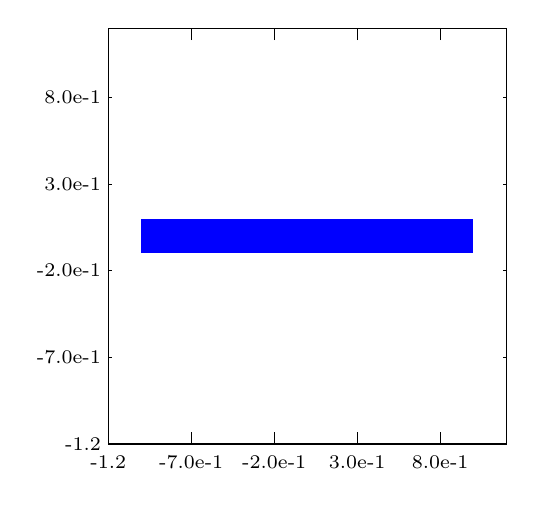
\begin{tikzpicture}[scale = 6,font=\scriptsize]
\draw (0.1148,0.085) rectangle (0.958,0.965);
\foreach \x/\label in {0.1148/-1.2,0.290466/-7.0e-1,0.466133/-2.0e-1,0.6418/3.0e-1,0.817466/8.0e-1} {
  \foreach \y in {0.94,0.085} \draw (\x,\y) -- (\x,\y+0.025);
  \node [below] at (\x,0.08) {\label};
}
\foreach \y/\label in {0.0849996/-1.2,0.268333/-7.0e-1,0.451666/-2.0e-1,0.635/3.0e-1,0.818333/8.0e-1} {
  \foreach \x in {0.951,0.1148} \draw (\x,\y) -- (\x+0.007,\y);
  \node [left] at (0.12,\y) {\label};
}
\fill [blue] (0.185067,0.488333) rectangle (0.887733,0.561667);
\end{tikzpicture}
\hspace{1cm}
% polygon
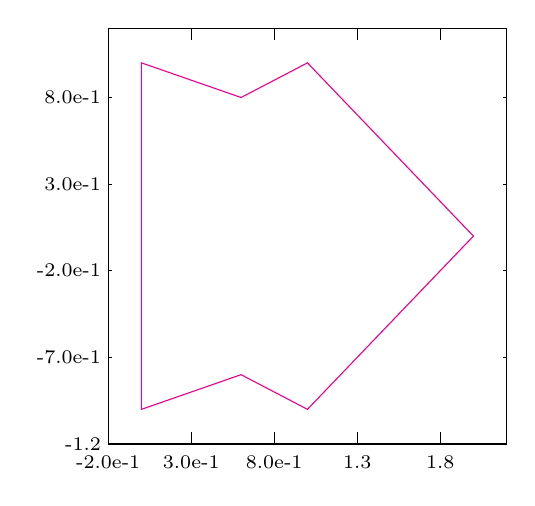
\begin{tikzpicture}[scale = 6,font=\scriptsize]
\draw (0.1148,0.085) rectangle (0.958,0.965);
\foreach \x/\label in {0.1148/-2.0e-1,0.290466/3.0e-1,0.466133/8.0e-1,0.6418/1.3,0.817466/1.8} {
  \foreach \y in {0.94,0.085} \draw (\x,\y) --(\x,\y+0.025);
  \node [below] at (\x,0.08) {\label};
}
\foreach \y/\label in {0.0849996/-1.2,0.268333/-7.0e-1,0.451666/-2.0e-1,0.635/3.0e-1,0.818333/8.0e-1} {
  \foreach \x in {0.951,0.1148} \draw (\x,\y) --(\x+0.007,\y);
  \node [left] at (0.12,\y) {\label};
}
\draw [magenta] (0.185067,0.891667) -- (0.185067,0.158333) -- (0.395867,0.231667) -- (0.5364,0.158333) -- (0.887733,0.525) -- (0.5364,0.891667) -- (0.395867,0.818333) -- cycle;
\end{tikzpicture}
\\[8mm]
% ellipse
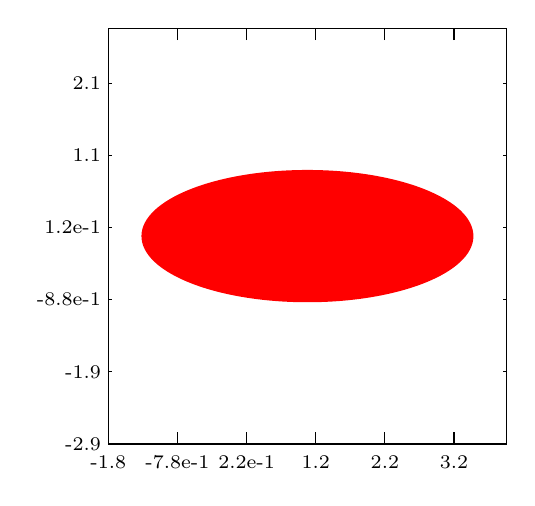
\begin{tikzpicture}[scale = 6,font=\scriptsize]
\draw (0.1148,0.085) rectangle (0.958,0.965);
\foreach \x/\label in {0.1148/-1.8,0.261189/-7.8e-1,0.407578/2.2e-1,0.553966/1.2,0.700355/2.2,0.846744/3.2} {
  \foreach \y in {0.94,0.085} \draw (\x,\y) --(\x,\y+0.025);
  \node [below] at (\x,0.08) {\label};
}
\foreach \y/\label in {0.0849996/-2.9,0.237777/-1.9,0.390555/-8.8e-1,0.543333/1.2e-1,0.696111/1.1,0.848888/2.1} {
  \foreach \x in {0.951,0.1148} \draw (\x,\y) --(\x+0.007,\y);
  \node [left] at (0.12,\y) {\label};
}
\fill [red] (0.5364,0.525) circle [x radius=0.351333,y radius=0.14];
\end{tikzpicture}
\hspace{1cm}
% ring
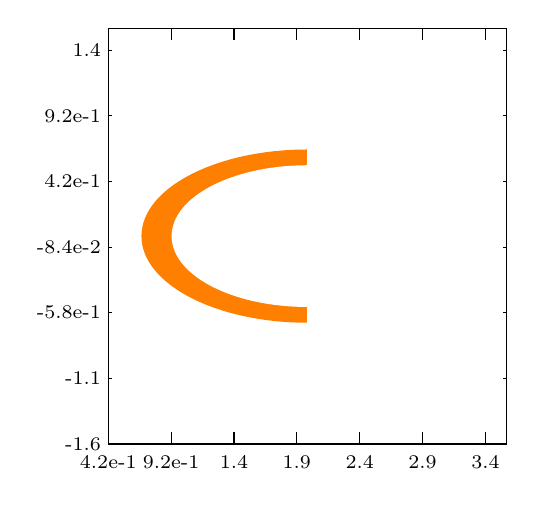
\begin{tikzpicture}[scale = 6,font=\scriptsize]
\draw (0.1148,0.085) rectangle (0.958,0.965);
\foreach \x/\label in {0.1148/4.2e-1,0.247881/9.2e-1,0.380962/1.4,0.514043/1.9,0.647123/2.4,0.780204/2.9,0.913285/3.4} {
  \foreach \y in {0.94,0.085} \draw (\x,\y) --(\x,\y+0.025);
  \node [below] at (\x,0.08) {\label};
}
\foreach \y/\label in {0.0849996/-1.6,0.223888/-1.1,0.362777/-5.8e-1,0.501666/-8.4e-2,0.640555/4.2e-1,0.779444/9.2e-1,0.918333/1.4} {
  \foreach \x in {0.951,0.1148} \draw (\x,\y) --(\x+0.007,\y);
  \node [left] at (0.12,\y) {\label};
}
\fill [color=orange] (0.5364,0.525) circle [x radius=0.351333,y radius=0.183333];
\fill [color=white] (0.5364,0.525) circle [x radius=0.287455,y radius=0.15];
\fill [color=white] (0.5364,0.158333) rectangle (0.9,0.784272);
\end{tikzpicture}
\caption{\label{fig:rg}Sample regions defined via the \ident{RG} class: interval (top left), polygon (top right), ellipse (bottom left), and ring (bottom right). These plots can be generated at run time by adding the command-line option \texttt{-rg\_view draw}.}
\end{figure}

Sometimes it is useful to specify the complement of a certain region, e.g., the part of the complex plane outside an ellipse. This can be achieved with
        \findex{RGSetComplement}
        \begin{Verbatim}[fontsize=\small]
        RGSetComplement(RG rg,PetscBool flg)
        \end{Verbatim}
or in the command line with \Verb!-rg_complement!.

By default, a newly created \ident{RG} object that is not set a type nor parameters must represent the whole complex plane (the same as \texttt{RGINTERVAL} with values $[-\infty,+\infty]\times[-\infty,+\infty]$). We call this the \emph{trivial} region, and provide a function to test this situation:
        \findex{RGIsTrivial}
        \begin{Verbatim}[fontsize=\small]
        RGIsTrivial(RG rg,PetscBool *trivial)
        \end{Verbatim}

Another useful operation is to check whether a given point of the complex plane is inside the region or not:
        \findex{RGCheckInside}
        \begin{Verbatim}[fontsize=\small]
        RGCheckInside(RG rg,PetscInt n,PetscScalar *ar,PetscScalar *ai,PetscInt *inside)
        \end{Verbatim}
Note that the point is represented as two \texttt{PetscScalar}'s, similarly to eigenvalues in \slepc.

\begin{table}
\centering
{\small \begin{tabular}{lll}
                       &                     & {\footnotesize Options} \\
Region Type            & \ident{RGType}      & {\footnotesize Database Name}\\\hline
(Generalized) Interval & \texttt{RGINTERVAL} & \texttt{interval} \\
Polygon                & \texttt{RGPOLYGON}  & \texttt{polygon} \\
Ellipse                & \texttt{RGELLIPSE}  & \texttt{ellipse} \\
Ring                   & \texttt{RGRING}     & \texttt{ring} \\\hline
\end{tabular} }
\caption{\label{tab:rg}Regions available as \ident{RG} objects.}
\end{table}

%---------------------------------------------------
\section{Directory Structure}

The directory structure of the \slepc software is very similar to that in \petsc. The root directory of \slepc contains the following directories:
\begin{description}
\item[\texttt{lib/slepc/conf}] - Directory containing the base \slepc makefile, to be included in application makefiles.
\item[\texttt{config}] - \slepc configuration scripts.
\item[\texttt{docs}] - All documentation for \slepc, including this manual. The subdirectory \texttt{manualpages} contains the on-line manual pages of each \slepc routine.
\item[\texttt{include}] - All include files for \slepc. The following subdirectories exist:
\begin{description}
\setlength{\itemsep}{0mm}
\item[\texttt{slepc/finclude}] - include files for Fortran programmers.
\item[\texttt{slepc/private}] - include files containing implementation details, for developer use only.
\end{description}
\item[\texttt{share/slepc}] - Common files, including:
\begin{description}
\setlength{\itemsep}{0mm}
\item[\texttt{datafiles}] - data files used by some examples.
%\item[\texttt{matlab}] - Matlab interface and examples.
\end{description}
\item[\texttt{src}] - The source code for all \slepc components, which currently includes:
\begin{description}
\setlength{\itemsep}{0mm}
\item[\texttt{sys}] - system-related routines and auxiliary classes \texttt{bv}, \texttt{ds}, \texttt{fn}, \texttt{rg}, \texttt{st}.
\item[\texttt{eps}] - eigenvalue problem solver.
\item[\texttt{svd}] - singular value decomposition solver.
\item[\texttt{pep}] - polynomial eigenvalue problem solver.
\item[\texttt{nep}] - nonlinear eigenvalue problem solver.
\item[\texttt{mfn}] - matrix function.
\item[\texttt{lme}] - linear matrix equations.
\end{description}
\item[\texttt{\$PETSC\_ARCH}] - For each value of \ident{PETSC\_ARCH}, a directory exists containing files generated during installation of that particular configuration. The following subdirectories exist:
\begin{description}
\setlength{\itemsep}{0mm}
\item[\texttt{lib}] - all the generated libraries.
\item[\texttt{lib/slepc/conf}] - configuration parameters and log files.
\item[\texttt{include}] - automatically generated include files, such as Fortran 90 \texttt{*.mod} files.
\end{description}
\end{description}

Each \slepc source code component directory has the following subdirectories:
\begin{description}
\item[\texttt{interface}] - The calling sequences for the abstract interface to the components. Code here does not know about particular implementations.
\item[\texttt{impls}] - Source code for the different implementations.
\item[\texttt{tutorials}] - Example programs intended for learning to use \slepc.
\item[\texttt{tests}] - Example programs used by testing scripts.
\end{description}

%---------------------------------------------------
%\section{Auxiliary Components}
%\label{sec:aux}

%The previous section includes a list of subdirectories, each of them representing a \slepc component. Most of these components have been treated in previous chapters. Here we include a brief report about two auxiliary components, \ident{BV} and \ident{DS}, that are not normally required by final users, but provide important operations to high level solvers such \ident{EPS}.

%\subsection{BV: Basis Vectors}

%\subsection{DS: Direct Solver (or Dense System)}

%---------------------------------------------------
\section{Wrappers to External Libraries}
\label{sec:wrap}

\slepc interfaces to several external libraries for the solution of eigenvalue problems. This section provides a short description of each of these packages as well as some hints for using them with \slepc, including pointers to the respective websites from which the software can be downloaded. The description may also include method-specific parameters, that can be set in the same way as other \slepc options, either procedurally or via the command-line.

In order to use \slepc together with an external library such as \arpack, one needs to do the following.
\begin{enumerate}
\item Install the external software, with the same compilers and MPI that will be used for \petsc/\slepc.
\item Enable the utilization of the external software from \slepc by specifying configure options as explained in \S\ref{sec:opt-inst}.
 \item Build the \slepc libraries.
\item Use the runtime option \Verb!-eps_type <type>! to select the solver.
\end{enumerate}

Exceptions to the above rule are \lapack, which should be enabled during \petsc's configuration, and \blopex, that must be installed with \Verb!--download-blopex! in \slepc's configure. Other packages also support the download option.

\subsection*{\underline{\lapack}}
\begin{description}
\setlength{\itemsep}{0pt}
\item[References.]\citep{Anderson:1999:LUG}.
\item[Website.] \url{https://www.netlib.org/lapack}.
\item[Version.] 3.0 or later.
\item[Summary.] \lapack\ (Linear Algebra PACKage) is a software package for the solution of many different dense linear algebra problems, including various types of eigenvalue problems and singular value decompositions.

\slepc explicitly creates the operator matrix in dense form and then the appropriate \lapack driver routine is invoked. Therefore, this interface should be used only for testing and validation purposes and not in a production code. The operator matrix is created by applying the operator to the columns of the identity matrix.

\item[Installation.]
The \slepc interface to \lapack can be used directly. If \slepc's configure script complains about missing \lapack functions, then configure \petsc with option \texttt{-{}-download-f2cblaslapack}.
\end{description}

\subsection*{\underline{\arpack}}
\begin{description}
\setlength{\itemsep}{0pt}
\item[References.]\citep{Lehoucq:1998:AUG}, \citep{Maschhoff:1996:PEP}.
\item[Website.] \url{https://github.com/opencollab/arpack-ng}.
\item[Version.] Release 2 (plus patches).
\item[Summary.] \arpack\ (ARnoldi PACKage) is a software package for the computation of a few eigenvalues and corresponding eigenvectors of a general $n\times n$ matrix $A$. It is most appropriate for large sparse or structured matrices, where structured means that a matrix-vector product $w \leftarrow Av$ requires order $n$ rather than the usual order $n^2$ floating point operations.

\arpack\ is based upon an algorithmic variant of the Arnoldi process called the Implicitly Restarted Arnoldi Method (IRAM). When the matrix $A$ is symmetric it reduces to a variant of the Lanczos process called the Implicitly Restarted Lanczos Method (IRLM). These variants may be viewed as a synthesis of the Arnoldi/Lanczos process with the Implicitly Shifted QR technique that is suitable for large scale problems.

It can be used for standard and generalized eigenvalue problems, both in real and complex arithmetic. It is implemented in Fortran 77 and it is based on the reverse communication interface. A parallel version, \parpack, is available with support for both MPI and BLACS.
\item[Installation.]
To install from the original website: first of all, unpack \texttt{arpack96.tar.gz} and also the patch file \texttt{patch.tar.gz}. If you plan to use the parallel version, extract also the contents of the file \texttt{parpack96.tar.gz} together with the patches \texttt{ppatch.tar.gz} (make sure you delete any \texttt{mpif.h} files that could exist in the directory tree). After setting all the directories, modify the \texttt{ARmake.inc} file and then compile the software with \texttt{make all}. It is recommended that \arpack is installed with its own \lapack version since it may give unexpected results with more recent versions of \lapack.

Alternatively, one can use the \textsc{arpack-ng} distribution, available in \texttt{github.com}, that supports \texttt{configure}+\texttt{make} for installation. Also, \slepc's \texttt{configure} allows to download this version automatically via the \texttt{-{}-download-arpack} option.

It is possible to configure \slepc with the serial version of \arpack. For this, you have to configure \petsc with the option \texttt{-{}-with-mpi=0}.
\end{description}

\subsection*{\underline{\primme}}
\begin{description}
\setlength{\itemsep}{0pt}
\item[References.]\citep{Stathopoulos:2010:PMS}.
\item[Website.] \url{https://www.cs.wm.edu/~andreas/software}.
\item[Version.] 3.2.
\item[Summary.] \primme (PReconditioned Iterative MultiMethod Eigensolver) is a C library for finding a number of eigenvalues and their corresponding eigenvectors of a real symmetric (or complex Hermitian) matrix. This library provides a multimethod eigensolver, based on Davidson/Jacobi-Davidson. Particular methods include GD+1, JDQMR, and LOBPCG. It supports preconditioning as well as the computation of interior eigenvalues.
\item[Installation.] Type \texttt{make lib} after customizing the file \texttt{Make\_flags} appropriately. Alternatively, the \texttt{-{}-download-primme} option is also available in \slepc's \texttt{configure}.
\item[Specific options.] Since PRIMME contains preconditioned solvers, the \slepc interface uses \ident{STPRECOND}, as described in \ref{sec:precond}.

The \slepc interface to this package allows the user to specify the maximum allowed block size with the function \ident{EPSPRIMMESetBlockSize} or at run time with the option \Verb!-eps_primme_blocksize <size>!.
For changing the particular algorithm within \primme, use the function \ident{EPSPRIMMESetMethod}.

\primme also provides a solver for the singular value decomposition that is interfaced in \slepc's \ident{SVD}, see chapter \ref{cap:svd}.
\end{description}

\subsection*{\underline{\evsl}}
\begin{description}
\setlength{\itemsep}{0pt}
\item[References.]\citep{Li:2019:EVS}.
\item[Website.] \url{https://www-users.cs.umn.edu/~saad/software/EVSL/}.
\item[Summary.] \evsl is a sequential library that implements methods for computing all eigenvalues located in a given interval for real symmetric (standard or generalized) eigenvalue problems. Currently SLEPc only supports standard problems.
\item[Installation.] The option \texttt{-{}-download-evsl} is available in \slepc's configure for easy installation. Alternatively, one can use an already installed version.
\end{description}

\subsection*{\underline{\trlan}}
\begin{description}
\setlength{\itemsep}{0pt}
\item[References.]\citep{Wu:2000:TLM}.
\item[Website.] \url{https://sdm.lbl.gov/\~kewu/trlan.html}.
\item[Version.] 201009.
\item[Summary.] This package provides a Fortran 90 implementation of the dynamic thick-restart Lanczos algorithm. This is a specialized version of Lanczos that targets only the case in which one wants both eigenvalues and eigenvectors of a large real symmetric eigenvalue problem that cannot use the shift-and-invert scheme. In this case the standard non-restarted Lanczos algorithm requires to store a large number of Lanczos vectors, what can cause storage problems and make each iteration of the method very expensive.

\trlan{} requires the user to provide a matrix-vector multiplication routine. The parallel version uses MPI as the message passing layer.
\item[Installation.] To install this package, it is necessary to have access to a Fortran 90 compiler. The compiler name and the options used are specified in the file called \texttt{Make.inc}. To generate the library, type \texttt{make plib} in the \texttt{TRLan} directory. Alternatively, the \texttt{-{}-download-trlan} option is also available in \slepc's \texttt{configure}.

It is possible to configure \slepc with the serial version of \trlan (built with \texttt{make lib}). For this, you have to configure \petsc with the option \texttt{-{}-with-mpi=0}.
\end{description}

\subsection*{\underline{\blopex}}
\begin{description}
\setlength{\itemsep}{0pt}
\item[References.]\citep{Knyazev:2007:BLO}.
\item[Website.] \url{https://github.com/lobpcg/blopex}.
\item[Summary.] \blopex is a package that implements the Locally Optimal Block Preconditioned Conjugate Gradient (LOBPCG) method for computing several extreme eigenpairs of symmetric positive generalized eigenproblems. Numerical comparisons suggest that this method is a genuine analog for eigenproblems of the standard preconditioned conjugate gradient method for symmetric linear systems.
\item[Installation.] In order to use \blopex from \slepc, it necessary to install it during \slepc's configuration: \Verb!./configure --download-blopex!.
\item[Specific options.] Since BLOPEX contains preconditioned solvers, the \slepc interface uses \ident{STPRECOND}, as described in \ref{sec:precond}.
\end{description}

\subsection*{\underline{\scalapack}}
\begin{description}
\setlength{\itemsep}{0pt}
\item[References.]\citep{Blackford:1997:SUG}.
\item[Website.] \url{https://www.netlib.org/scalapack}.
\item[Summary.] \scalapack is a library of high-performance linear algebra routines for parallel distributed memory machines. It contains eigensolvers for dense Hermitian eigenvalue problems, as well as solvers for the (dense) SVD.
\item[Installation.] For using \scalapack from \slepc it is necessary to select it during configuration of \petsc.
\end{description}

\subsection*{\underline{\elpa}}
\begin{description}
\setlength{\itemsep}{0pt}
\item[References.]\citep{Auckenthaler:2011:ELP}.
\item[Website.] \url{https://elpa.mpcdf.mpg.de/}.
\item[Summary.] \elpa is a high-performance library for the parallel solution of dense symmetric (or Hermitian) eigenvalue problems on distributed memory computers. It uses a ScaLAPACK-compatible matrix distribution.
\item[Installation.] The \slepc wrapper to \elpa can be activated at configure time with the option \texttt{-{}-download\_elpa}, in which case \scalapack support must have been enabled during the configuration of \petsc.
\end{description}

\subsection*{\underline{\ksvd}}
\begin{description}
\setlength{\itemsep}{0pt}
\item[References.]\citep{Sukkari:2019:QDW}.
\item[Website.] \url{https://github.com/ecrc/ksvd/}.
\item[Summary.] \ksvd is a high performance software framework for computing a dense SVD on distributed-memory manycore systems. The \ksvd solver relies on the polar decomposition (PD) based on the QR Dynamically-Weighted Halley (QDWH) and ZOLO-PD algorithms.
\item[Installation.] The option \texttt{-{}-download-ksvd} is available in \slepc's configure for easy installation, which in turn requires adding \texttt{-{}-download-polar} and \texttt{-{}-download-elpa}.
\end{description}

\subsection*{\underline{\elemental}}
\begin{description}
\setlength{\itemsep}{0pt}
\item[References.]\citep{Poulson:2013:ELE}.
\item[Website.] \url{https://github.com/elemental/Elemental}.
\item[Summary.] \elemental is distributed-memory, arbitrary-precision, dense and sparse-direct linear algebra package. It contains eigensolvers for dense Hermitian eigenvalue problems, as well as solvers for the SVD.
\item[Installation.] For using \elemental from \slepc it is necessary to select it during configuration of \petsc.
\end{description}

\subsection*{\underline{\feast}}
\begin{description}
\setlength{\itemsep}{0pt}
\item[References.]\citep{Polizzi:2009:DAS}.
\item[Website.] \url{https://feast-solver.org/}.
\item[Summary.] \feast is a numerical library for solving the standard or generalized symmetric eigenvalue problem, and obtaining all the eigenvalues and eigenvectors within a given search interval. It is based on an innovative fast and stable numerical algorithm which deviates fundamentally from the traditional Krylov subspace based iterations or Davidson-Jacobi techniques. The FEAST algorithm takes its inspiration from the density-matrix representation and contour integration technique in quantum mechanics. Latest versions also support non-symmetric problems.
\item[Installation.] We only support the \feast implementation included in Intel MKL. For using it from \slepc it is necessary to configure \petsc with MKL by adding the corresponding option, e.g., \Verb!--with-blas-lapack-dir=$MKLROOT!.
\item[Specific options.] The \slepc interface to \feast allows the user to specify the number of contour integration points with the function \ident{EPSFEASTSetNumPoints} or at run time with the option \Verb!-eps_feast_num_points <n>!.
\end{description}

\subsection*{\underline{\chase}}
\begin{description}
\setlength{\itemsep}{0pt}
\item[References.]\citep{Winkelmann:2019:CCA}.
\item[Website.] \url{https://github.com/ChASE-library/ChASE}.
\item[Summary.] \chase is a modern and scalable library based on subspace iteration with polynomial acceleration to solve dense Hermitian (symmetric) algebraic eigenvalue problems, especially solving dense Hermitian eigenproblems arranged in a sequence. Novel to ChASE is the computation of the spectral estimates that enter in the filter and an optimization of the polynomial degree that further reduces the necessary floating-point operations.
\item[Installation.] Currently, the \chase interface in \slepc is based on the MPI version with block-cyclic distribution, i.e., \scalapack matrix storage, so it is necessary to enable \scalapack during configuration of \petsc.
\end{description}

%---------------------------------------------------
\section{Fortran Interface}
\label{sec:fortran}

\slepc provides an interface for Fortran programmers, very much like \petsc. As in the case of \petsc, there are slight differences between the C and Fortran \slepc interfaces, due to differences in Fortran syntax. For instance, the error checking variable is the final argument of all the routines in the Fortran interface, in contrast to the C convention of providing the error variable as the routine's return value.

The following is a Fortran example. It is the Fortran equivalent of the program given in \S\ref{sec:simpleex} and can be found in \Verb!${SLEPC_DIR}/src/eps/tutorials! (file \texttt{ex1f.F90}).
\MyVerbatimInput{ex1f.F90}

%---------------------------------------------------
%\section{Matlab Interface}
%\label{sec:matlab}
%
%Since version 3.2, \slepc includes an interface intended to make most of \slepc's functionality available from Matlab. It is experimental and needs further development, so users planning to use it seriously are recommended to contact the authors. Below are some guidelines for using this interface.
%
%First of all, \petsc must have been configured with the Matlab interface enabled. This can be done as follows (check \petsc documentation for details):
%       \begin{Verbatim}[fontsize=\small]
%       $ ./configure --with-matlab --with-matlab-engine --with-shared-libraries
%       \end{Verbatim}
%
%Once the \petsc and \slepc libraries have been built, one has to set Matlab's path to point to the directories containing Matlab classes: \Verb!$SLEPC_DIR/share/slepc/matlab/classes! and \Verb!$PETSC_DIR/share/slepc/matlab/classes!. Below we show a simple Matlab example (included in \slepc's distribution) that does this, and then solves a simple eigenproblem.
%\MyVerbatimInput{exEPS.m}



%---------------------------------------------------
\cleardoublepage
\fancyhead{}\fancyhead[LO,RE]{\nouppercase{\scriptsize \sffamily Bibliography}}
\addcontentsline{toc}{chapter}{Bibliography}

%\bibliographystyle{engnat}
%\bibliography{slepc}
%-------------------------------------------------------
% SLEPc Users Manual
%-------------------------------------------------------

\documentclass[titlepage,10pt,a4paper]{book}

\usepackage{xcolor}
\usepackage{graphicx}
\usepackage[square]{natbib}
\usepackage{fancyhdr}
\usepackage{fancyvrb}
\usepackage{caption}
\usepackage{xspace}
\usepackage{ae,aecompl}
\usepackage{amsmath,amssymb}
\usepackage{imakeidx}
\usepackage{hyperref}
\usepackage{titlesec}
\usepackage{tikz,pgfplots}

\makeindex

\hypersetup{
  colorlinks,
  linkcolor=purple,
  citecolor=violet,
  filecolor=blue,
  urlcolor=magenta,
  bookmarksnumbered,
  pdfstartview=FitH,
  pdftitle={SLEPc Users Manual},
  pdfauthor={J. E. Roman, C. Campos, L. Dalcin, E. Romero, A. Tomas},
  pdfsubject={SLEPc: Scalable Library for Eigenvalue Problem Computations},
  pdfkeywords={SLEPc, PETSc, eigenvalue problems}
}

\newcommand{\slepcversion}{3.23}
\newcommand{\slepchome}{https://slepc.upv.es}
\newcommand{\pack}[1]{{\sc #1}\index{\textsc{#1}}\xspace}
\newcommand{\packnoi}[1]{{\sc #1}\xspace}
\newcommand{\slepc}{\texorpdfstring{\packnoi{slep\rm c}}{{SLEPc}}}
\newcommand{\petsc}{\pack{pets\rm c}}
\newcommand{\blas}{\pack{blas}}
\newcommand{\lapack}{\pack{lapack}}
\newcommand{\arpack}{\pack{arpack}}
\newcommand{\parpack}{\pack{parpack}}
\newcommand{\trlan}{\pack{trlan}}
\newcommand{\primme}{\pack{primme}}
\newcommand{\blopex}{\pack{blopex}}
\newcommand{\scalapack}{\pack{scalapack}}
\newcommand{\elpa}{\pack{elpa}}
\newcommand{\elemental}{\pack{elemental}}
\newcommand{\evsl}{\pack{evsl}}
\newcommand{\feast}{\pack{feast}}
\newcommand{\ksvd}{\pack{ksvd}}
\newcommand{\chase}{\pack{chase}}
\newcommand{\mpich}{\pack{mpich}}
\newcommand{\expokit}{\pack{expokit}}
\newcommand{\rutina}[1]{\texttt{#1}\index{\texttt{#1}}}
\newcommand{\ident}[1]{\texttt{#1}\index{\texttt{#1}}}
\newcommand{\findex}[1]{\index{\texttt{#1}}}

\DeclareMathOperator{\rev}{rev}

%VerbatimEnvironment%
\fvset{numbers=left,numbersep=6pt,stepnumber=5}
\newcommand{\MyVerbatimInput}[1]{\fvset{fontsize=\scriptsize}%
  \VerbatimInput{#1}%
  \fvset{fontsize=\normalsize}%
}

\setlength{\textwidth}{14.5cm}
\setlength{\tabcolsep}{2mm}
\renewcommand{\arraystretch}{1.05}
\setcounter{tocdepth}{3}
\renewcommand{\captionlabelfont}{\sl\sffamily}
\makeatletter\@ifundefined{bibfont}{\newcommand{\bibfont}{\small}}{\renewcommand{\bibfont}{\small}}\makeatother

\titleformat{\chapter}[display]
  {\bfseries\Large}
  {\filleft\setlength{\fboxsep}{2mm}\fbox{\large\sc\chaptertitlename}\hspace*{-0.5mm}\setlength{\fboxsep}{4mm}\setlength{\fboxrule}{.5mm}\fbox{\Huge\bfseries\thechapter}}
  {4ex}
  {\huge\bf\sffamily
   \filright}
  [\hfill\rule{10cm}{1pt}]

\begin{document}

\title{
   \vspace*{-1cm}
   \framebox[12cm][l]{
   \includegraphics[height=1.4cm]{figures/upv}
   \hfill
   \parbox[b]{4cm}{\begin{flushright}\vspace*{-7mm}\normalsize\sl\sffamily
   Departamento de\\[-0.8mm] Sistemas Inform\'aticos\\[-0.8mm]
   y Computaci\'on\\[0.8mm]
   \vspace{-2.5mm}\end{flushright}}
   \raisebox{3mm}{\includegraphics[height=9mm,width=1.4cm]{figures/dsic}}
   }
   \\[2cm]
   \normalsize Technical Report DSIC-II/24/02
   \\[2cm]
   \vspace*{6mm}
   {\Large\bf\sffamily
   SLEPc Users Manual\\[2mm]}
   {\large\bf\sffamily
   Scalable Library for Eigenvalue Problem Computations}\\[2mm]
   \vspace*{6mm}
   \vspace*{6mm}
   \url{\slepchome}
   \\[6mm]
}

\author{
  Jose E. Roman\\
  Carmen Campos\\
  Lisandro Dalcin\\
  Eloy Romero\\
  Andr\'es Tom\'as\\[3mm]
}

\date{
   To be used with \slepc \slepcversion\\
   March, 2025
}

\hypersetup{pageanchor=false}
\begin{titlepage}
\maketitle
\end{titlepage}

\setlength{\textheight}{18cm}
\setlength{\oddsidemargin}{0.6cm}
\setlength{\evensidemargin}{0.6cm}
\setlength{\footskip}{2cm}
\setlength{\voffset}{1.3cm}

\pagestyle{empty}
\cleardoublepage
\hypersetup{pageanchor=true}

{
  \pagestyle{plain}
  \pagenumbering{roman}
%---------------------------------------------------
\subsection*{Abstract}

This document describes \slepc, the {\em Scalable Library for Eigenvalue Problem Computations}, a software package for the solution of large sparse eigenproblems on parallel computers. It can be used for the solution of various types of eigenvalue problems, including linear and nonlinear, as well as other related problems such as the singular value decomposition (see a summary of supported problem classes on page \pageref{tab:modules}). \slepc is a general library in the sense that it covers both Hermitian and non-Hermitian problems, with either real or complex arithmetic.

The emphasis of the software is on methods and techniques appropriate for problems in which the associated matrices are large and sparse, for example, those arising after the discretization of partial differential equations. Thus, most of the methods offered by the library are projection methods, including different variants of Krylov and Davidson iterations. In addition to its own solvers, \slepc provides transparent access to some external software packages such as \packnoi{arpack}. These packages are optional and their installation is not required to use \slepc, see \S\ref{sec:wrap} for details. Apart from the solvers, \slepc also provides built-in support for some operations commonly used in the context of eigenvalue computations, such as preconditioning or the shift-and-invert spectral transformation.

\slepc is built on top of \packnoi{pets\rm c}, the Portable, Extensible Toolkit for Scientific Computation \citep{Balay:PUM}. It can be considered an extension of \packnoi{pets\rm c} providing all the functionality necessary for the solution of eigenvalue problems. This means that \packnoi{pets\rm c} must be previously installed in order to use \slepc. \packnoi{pets\rm c} users will find \slepc very easy to use, since it enforces the same programming paradigm. Those readers that are not acquainted with \packnoi{pets\rm c} are highly recommended to familiarize with it before proceeding with \slepc.


\subsubsection*{How to Get \slepc}

All the information related to \slepc can be found at the following web site:
\begin{quote}
\begin{center}
\url{\slepchome}.
\end{center}
\end{quote}
The distribution file is available for download at this site. Other information is provided there, such as installation instructions and contact information. Instructions for installing the software can also be found in \S\ref{sec:inst}.

\packnoi{pets\rm c} can be downloaded from \url{https://petsc.org}.  \packnoi{pets\rm c} is supported, and information on contacting support can be found at that site.

\subsubsection*{Additional Documentation}

This manual provides a general description of \slepc. In addition, manual pages for individual routines are included in the distribution file in hypertext format, and are also available on-line at \url{\slepchome/documentation}. These manual pages provide hyperlinked access to the source code and enable easy movement among related topics. Finally, there are also several hands-on exercises available, which are intended for learning the basic concepts easily.

\subsubsection*{How to Read this Manual}

Users that are already familiar with \packnoi{pets\rm c} can read chapter \ref{cap:int} very fast. Section \ref{sec:eig} provides a brief overview of eigenproblems and the general concepts used by eigensolvers, so it can be skipped by experienced users. Chapters \ref{cap:eps}--\ref{cap:mfn} describe the main \slepc functionality. Some of them include an advanced usage section that can be skipped at a first reading. Finally, chapter \ref{cap:add} contains less important, additional information.

%\subsubsection*{What's New}
%
%The major changes in the Users Manual with respect to the previous version are:
%\begin{itemize}
%\setlength{\itemsep}{-2pt}
%\item New section \S\ref{sec:gsvd} related to the generalized singular value decomposition (GSVD). The rest of Ch.~\ref{cap:svd} has been slightly modified to cover the new GSVD functionality.
%\end{itemize}

\subsubsection*{\slepc Technical Reports}

The information contained in this manual is complemented by a set of Technical Reports, which provide technical details that normal users typically do not need to know but may be useful for experts in order to identify the particular method implemented in \slepc. These reports are not included in the \slepc distribution file but can be accessed via the \slepc web site. A \hyperlink{str}{list of available reports} is included at the end of the Bibliography.


\subsubsection*{Acknowledgments}

%We thank all the \packnoi{pets\rm c} team for their help and support. Without their continued effort invested in \packnoi{pets\rm c}, \slepc would not have been possible.
% We also thank Osni Marques and Tony Drummond for helping us raise awareness of \slepc in the context of the ACTS project.

The current version contains code contributed by:
A.\ Lamas Davi\~{n}a (CUDA code),
F.\ Alvarruiz (restarted Lanczos for the GSVD, structured BSE solvers),
B.\ Mellado-Pinto (structured BSE solvers),
Y.\ Maeda, T.\ Sakurai (CISS solvers),
M.\ Moldaschl, W.\ Gansterer (BDC subroutines),
F.\ Kong (nonlinear inverse iteration),
H.\ Fang, Y. Saad (\textsc{filtlan} polynomial filter).

Development of \slepc has been partially funded by the following grants:
\begin{itemize}
\setlength{\itemsep}{-2pt}
\item Innovation Study ISOLV-BSE has received funding through the Inno4scale project, which is funded by the European High-Performance Computing Joint Undertaking (JU) under Grant Agreement No 101118139. The JU receives support from the European Union's Horizon Europe Programme.
\item Agencia Estatal de Investigaci\'on (Spain), grant no.\ PID2022-139568NB-I00, PI: Jos\'e E. Rom\'an.
\item Agencia Estatal de Investigaci\'on (Spain), grant no.\ PID2019-107379RB-I00, PI: Jos\'e E. Rom\'an.
\item Agencia Estatal de Investigaci\'on (Spain), grant no.\ TIN2016-75985-P, PI: Jos\'e E. Rom\'an.
\item Ministerio de Econom\'{\i}a y Comp.\ (Spain), grant no.\ TIN2013-41049-P, PI: Jos\'e E. Rom\'an.
\item Ministerio de Ciencia e Innovaci\'on (Spain), grant no.\ TIN2009-07519, PI: Jos\'e E. Rom\'an.
\item Valencian Regional Government, grant no.\ GV06/091, PI: Jos\'e E. Rom\'an.
\item Valencian Regional Government, grant no.\ CTIDB/2002/54, PI: Vicente Hern\'andez.
\end{itemize}

\subsubsection*{License and Copyright}

Starting from version 3.8, \slepc is released under a 2-clause BSD license (see \texttt{LICENSE} file).

\begin{quote}
\begin{sffamily}
Copyright 2002--2025 Universitat Polit\`ecnica de Valencia, Spain
\end{sffamily}
\end{quote}

%---------------------------------------------------
\newpage
\subsubsection*{Supported Problem Classes}

The following table provides an overview of the functionality offered by \slepc, organized by problem classes.

\begin{table}[h]
\label{tab:modules}
\centering
{\small \begin{tabular}{lccc}
Problem class                 & Model equation  & Module       & Chapter \\\hline
Linear eigenvalue problem     & $Ax=\lambda x,\quad Ax=\lambda Bx$ & \texttt{EPS} & \ref{cap:eps} \\
Quadratic eigenvalue problem  & $(K+\lambda C+\lambda^2M)x=0$ & -- & -- \\
Polynomial eigenvalue problem & $(A_0+\lambda A_1+\cdots+\lambda^dA_d)x=0$ & \texttt{PEP} & \ref{cap:pep} \\
Nonlinear eigenvalue problem  & $T(\lambda)x=0$ & \texttt{NEP} & \ref{cap:nep} \\\hline
Singular value decomposition  & $Av=\sigma u$   & \texttt{SVD} & \ref{cap:svd} \\
Matrix function (action of)   & $y=f(A)v$   & \texttt{MFN} & \ref{cap:mfn} \\
Linear matrix equation        & $AXE+DXB=C$   & \texttt{LME} & See notes \\\hline
\end{tabular} }
\end{table}

\noindent In order to solve a given problem, one should create a solver object corresponding to the solver class (module) that better fits the problem (the less general one; e.g., we do not recommend using \texttt{NEP} to solve a linear eigenproblem).\\[3mm]

\noindent Notes:\vspace{-2mm}
\begin{itemize}
\setlength{\itemsep}{-2pt}
\item Most users are typically interested in linear eigenproblems only.
\item In each problem class there may exist several subclasses (problem types in \slepc terminology), for instance symmetric-definite generalized eigenproblem in \texttt{EPS}.
\item The solver class (module) is named after the problem class. For historical reasons, the one for linear eigenvalue problems is called \texttt{EPS} rather than \texttt{LEP}.
\item In addition to the SVD shown in the table, the \texttt{SVD} module also supports other related problems such as the GSVD and the HSVD.
\item In previous \slepc versions there was a \texttt{QEP} module for quadratic eigenproblems. It has been replaced by \texttt{PEP}. %See \S\ref{sec:qeppep} for upgrading application code that used \texttt{QEP}.
\item For the action of a matrix function (\texttt{MFN}), in \slepc we focus on methods that are closely related to methods for eigenvalue problems.
\item The solver class \texttt{LME} is still experimental and it is not covered in this manual yet.
\end{itemize}

%---------------------------------------------------
  \setlength{\parskip}{0cm}
  \tableofcontents
}
\cleardoublepage
\pagenumbering{arabic}
\pagestyle{fancy}
\renewcommand{\chaptermark}[1]{\markboth{\scriptsize \sffamily {\bfseries\chaptername\ \thechapter.} #1}{}}
\renewcommand{\sectionmark}[1]{\markright{\scriptsize \sffamily {\bfseries\thesection.} #1}{}}
\fancyhead{}
\fancyhead[LE,RO]{\nouppercase{\rightmark}}
\fancyhead[LO,RE]{\nouppercase{\leftmark}}
\fancyfoot[C]{\scriptsize --- \thepage\ ---}
\renewcommand{\headrulewidth}{0.2pt}
\renewcommand{\footrulewidth}{0.2pt}

%-------------------------------------------------------
% SLEPc Users Manual
%-------------------------------------------------------
\chapter{\label{cap:int}Getting Started}
%-------------------------------------------------------

\noindent \slepc, the {\em Scalable Library for Eigenvalue Problem Computations}, is a software library for the solution of large sparse eigenvalue problems on parallel computers.

Together with linear systems of equations, eigenvalue problems are a very important class of linear algebra problems. The need for the numerical solution of these problems arises in many situations in science and engineering, in problems associated with stability and vibration analysis in practical applications. These are usually formulated as large sparse eigenproblems.

Computing eigenvalues is essentially more difficult than solving linear systems of equations. This has resulted in a very active research activity in the area of computational methods for eigenvalue problems in the last years, with many remarkable achievements.  However, these state-of-the-art methods and algorithms are not easily transferred to the scientific community, and, apart from a few exceptions, most user still rely on simpler, well-established techniques.

The reasons for this situation are diverse. First, new methods are increasingly complex and difficult to implement and therefore robust implementations must be provided by computational specialists, for example as software libraries. The development of such libraries requires to invest a lot of effort but sometimes they do not reach normal users due to a lack of awareness.

In the case of eigenproblems, using libraries is not straightforward. It is usually recommended that the user understands how the underlying algorithm works and typically the problem is successfully solved only after several cycles of testing and parameter tuning. Methods are often specific for a certain class of eigenproblems and this leads to an explosion of available algorithms from which the user has to choose. Not all these algorithms are available in the form of software libraries, even less frequently with parallel capabilities.

Another difficulty resides in how to represent the operator matrix. Unlike in dense methods, there is no widely accepted standard for basic sparse operations in the spirit of \blas. This is due to the fact that sparse storage is more complicated, admitting of more variation, and therefore less standardized. For this reason, sparse libraries have an added level of complexity. This holds even more so in the case of parallel distributed-memory programming, where the data of the problem have to be distributed across the available processors.

The first implementations of algorithms for sparse matrices required a prescribed storage format for the sparse matrix, which is an obvious limitation. An alternative way of matrix representation is by means of a user-provided subroutine for the matrix-vector product. Apart from being format-independent, this approach allows the solution of problems in which the matrix is not available explicitly. The drawback is the restriction to a fixed-prototype subroutine.

A better solution for the matrix representation problem is the well-known reverse communication interface, a technique that allows the development of iterative methods disregarding the implementation details of various operations. Whenever the iterative method subroutine needs the results of one of the operations, it returns control to the user's subroutine that called it. The user's subroutine then invokes the module that performs the operation. The iterative method subroutine is invoked again with the results of the operation.

Several libraries with any of the interface schemes mentioned above are publicly available. For a survey of such software see the \slepc Technical Report \hyperlink{str}{[STR-6]}, ``A Survey of Software for Sparse Eigenvalue Problems'', and references therein. Some of the most recent libraries are even prepared for parallel execution (some of them can be used from within \slepc, see \S\ref{sec:wrap}). However, they still lack some flexibility or require too much programming effort from the user, especially in the case that the eigensolution requires to employ advanced techniques such as spectral transformations or preconditioning.

A further obstacle appears when these libraries have to be used in the context of large software projects carried out by inter-disciplinary teams. In this scenery, libraries must be able to interoperate with already existing software and with other libraries. In order to cope with the complexity associated with such projects, libraries must be designed carefully in order to overcome hurdles such as different storage formats or programming languages. In the case of parallel software, care must be taken also to achieve portability to a wide range of platforms with good performance and still retain flexibility and usability.

%---------------------------------------------------
\section{SLEPc and PETSc}

The \slepc library is an attempt to provide a solution to the situation described in the previous paragraphs. It is intended to be a general library for the solution of eigenvalue problems that arise in different contexts, covering standard and generalized problems, both Hermitian and non-Hermitian, with either real or complex arithmetic. Issues such as usability, portability, efficiency and interoperability are addressed, and special emphasis is put on flexibility, providing data-structure neutral implementations and multitude of run-time options. \slepc offers a growing number of eigensolvers as well as interfaces to integrate well-established eigenvalue packages such as \arpack. In addition to the linear eigenvalue problem, \slepc also includes other solver classes for nonlinear eigenproblems, SVD and the computation of the action of a matrix function.

\slepc is based on \petsc, the Portable, Extensible Toolkit for Scientific Computation \citep{Balay:PUM}, and, therefore, a large percentage of the software complexity is avoided since many \petsc developments are leveraged, including matrix storage formats and linear solvers, to name a few. \slepc focuses on high level features for eigenproblems, structured around a few object classes as described below.

\petsc uses modern programming paradigms to ease the development of large-scale scientific application codes in Fortran, C, and C++ and provides a powerful set of tools for the numerical solution of partial differential equations and related problems on high-performance computers. Its approach is to encapsulate mathematical algorithms using object-oriented programming techniques, which allow to manage the complexity of efficient numerical message-passing codes. All the \petsc software is free and used around the world in a variety of application areas.

The design philosophy is not to try to completely conceal parallelism from the application programmer. Rather, the user initiates a combination of sequential and parallel phases of computations, but the library handles the detailed message passing required during the coordination of computations. Some of the design principles are described in \citep{Balay:1997:EMP}.

\petsc is built around a variety of data structures and algorithmic objects. The application programmer works directly with these objects rather than concentrating on the underlying data structures. Each component manipulates a particular family of objects (for instance, vectors) and the operations one would like to perform on the objects. The three basic abstract data objects are index sets, vectors and matrices. Built on top of this foundation are various classes of solver objects, which encapsulate virtually all information regarding the solution procedure for a particular class of problems, including the local state and various options such as convergence tolerances, etc.

\slepc can be considered an extension of \petsc providing all the functionality necessary for the solution of eigenvalue problems. Figure \ref{fig:slepc} shows a diagram of all the different objects included in \petsc (on the left) and those added by \slepc (on the right). \petsc is a prerequisite for \slepc and users should be familiar with basic concepts such as vectors and matrices in order to use \slepc. Therefore, together with this manual we recommend to use the \petsc Users Manual \citep{Balay:PUM}.

\begin{figure}[t]
\centering
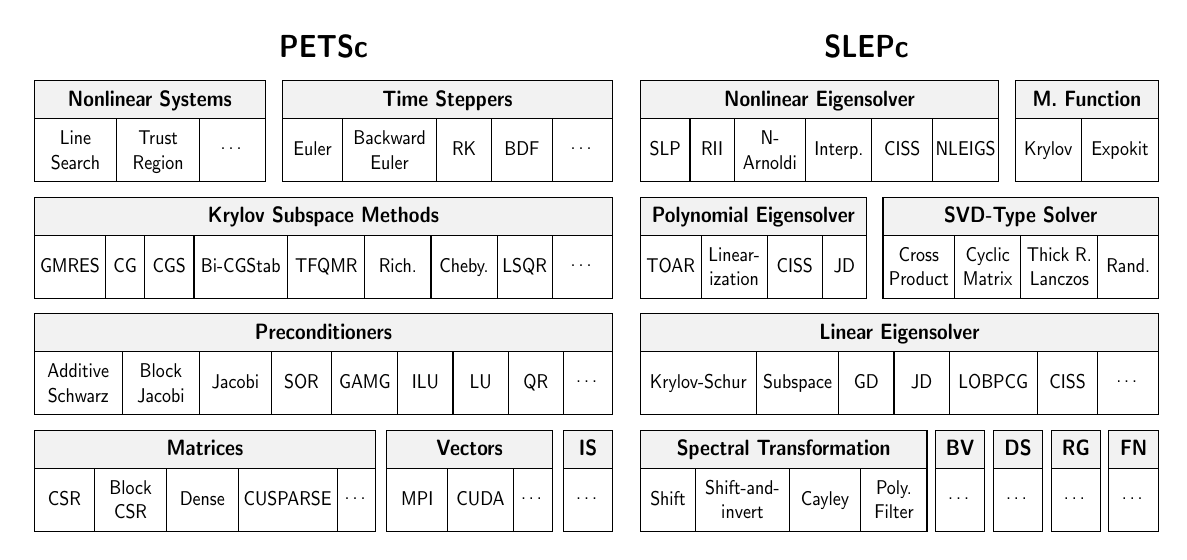
\begin{tikzpicture}[xscale=0.7,yscale=0.8]
  \tikzstyle{interface}=[fill=black!5,font=\sffamily\bfseries,text depth=.25ex]
  \tikzstyle{implem}=[font=\sffamily\small,text badly centered]
  \tikzstyle{every node}=[transform shape]
  \tikzstyle{onel}=[text depth=.25ex]
  \def\levsep{1.85} % separation of levels
  \def\hint{0.6} % height interface
  \def\himp{1} % height implementation
  \node[above,text centered,font=\sffamily\bfseries\Large] at (5.25,5*\levsep) {PETSc};
  \draw[interface] (0,\levsep+\himp) rectangle node {Matrices} +(6.2,\hint);
  \draw[implem] (0,\levsep) rectangle node[onel] {CSR} ++(1.1,1) ++(0,-1)
                rectangle node[text width=1.3cm] {Block CSR} ++(1.3,1) ++(0,-1)
                rectangle node[onel] {Dense} ++(1.3,1) ++(0,-1)
                rectangle node[onel] {CUSPARSE} ++(1.8,1) ++(0,-1)
                rectangle node[onel] {\dots} ++(.7,1);
  \draw[interface] (6.4,\levsep+\himp) rectangle node {Vectors} +(3,\hint);
  \draw[implem] (6.4,\levsep) rectangle node[onel] {MPI} ++(1.1,1) ++(0,-1)
                      rectangle node[onel] {CUDA} ++(1.2,1) ++(0,-1)
                      rectangle node[onel] {\dots} ++(.7,1);
  \draw[interface] (9.6,\levsep+\himp) rectangle node {IS} +(.9,\hint);
  \draw[implem] (9.6,\levsep) rectangle node[onel] {\dots} ++(.9,1);
  \draw[interface] (0,2*\levsep+\himp) rectangle node {Preconditioners} +(10.5,\hint);
  \draw[implem] (0,2*\levsep) rectangle node[text width=1.6cm] {Additive Schwarz} ++(1.6,1) ++(0,-1)
                rectangle node[text width=1.2cm] {Block Jacobi} ++(1.4,1) ++(0,-1)
                rectangle node[onel] {Jacobi} ++(1.3,1) ++(0,-1)
                rectangle node[onel] {SOR} ++(1.1,1) ++(0,-1)
                rectangle node[onel] {GAMG} ++(1.2,1) ++(0,-1)
                rectangle node[onel] {ILU} ++(1,1) ++(0,-1)
                rectangle node[onel] {LU} ++(1,1) ++(0,-1)
                rectangle node[onel] {QR} ++(1,1) ++(0,-1)
                rectangle node[onel] {\dots} ++(.9,1);
  \draw[interface] (0,3*\levsep+\himp) rectangle node {Krylov Subspace Methods} +(10.5,\hint);
  \draw[implem] (0,3*\levsep) rectangle node[onel] {GMRES} ++(1.3,1) ++(0,-1)
                rectangle node[onel] {CG} ++(0.7,1) ++(0,-1)
                rectangle node[onel] {CGS} ++(0.9,1) ++(0,-1)
                rectangle node[onel] {Bi-CGStab} ++(1.7,1) ++(0,-1)
                rectangle node[onel] {TFQMR} ++(1.4,1) ++(0,-1)
                rectangle node[onel] {Rich.} ++(1.2,1) ++(0,-1)
                rectangle node[onel] {Cheby.} ++(1.2,1) ++(0,-1)
                rectangle node[onel] {LSQR} ++(1,1) ++(0,-1)
                rectangle node[onel] {\dots} ++(1.1,1);
  \draw[interface] (0,4*\levsep+\himp) rectangle node {Nonlinear Systems} +(4.2,\hint);
  \draw[implem] (0,4*\levsep) rectangle node[text width=1.2cm] {Line Search} ++(1.5,1) ++(0,-1)
                rectangle node[text width=1.2cm,yshift=-1pt] {Trust Region} ++(1.5,1) ++(0,-1)
                rectangle node[onel] {\dots} ++(1.2,1);
  \draw[interface] (4.5,4*\levsep+\himp) rectangle node {Time Steppers} +(6,\hint);
  \draw[implem] (4.5,4*\levsep) rectangle node[onel] {Euler} ++(1.1,1) ++(0,-1)
                rectangle node[text width=1.5cm] {Backward Euler} ++(1.7,1) ++(0,-1)
                rectangle node[onel] {RK} ++(1.0,1) ++(0,-1)
                rectangle node[onel] {BDF} ++(1.1,1) ++(0,-1)
                rectangle node[onel] {\dots} ++(1.1,1);
  \node[above,text centered,font=\sffamily\bfseries\Large] at (15.1,5*\levsep) {SLEPc};
  \draw[interface] (11,4*\levsep+\himp) rectangle node {Nonlinear Eigensolver} +(6.5,\hint);
  \draw[implem] (11,4*\levsep) rectangle node[onel] {SLP} ++(.9,1) ++(0,-1)
                rectangle node[onel] {RII} ++(.8,1) ++(0,-1)
                rectangle node[text width=1.2cm] {N-Arnoldi} ++(1.3,1) ++(0,-1)
                rectangle node[onel] {Interp.} ++(1.2,1) ++(0,-1)
                rectangle node[onel] {CISS} ++(1.1,1) ++(0,-1)
                rectangle node[onel] {NLEIGS} ++(1.2,1);
  \draw[interface] (17.8,4*\levsep+\himp) rectangle node {M.~Function} +(2.6,\hint);
  \draw[implem] (17.8,4*\levsep) rectangle node[onel] {Krylov} ++(1.2,1) ++(0,-1)
                rectangle node[onel] {Expokit} ++(1.4,1);
  \draw[interface] (11,3*\levsep+\himp) rectangle node {Polynomial Eigensolver} +(4.1,\hint);
  \draw[implem] (11,3*\levsep) rectangle node[onel] {TOAR} ++(1.1,1) ++(0,-1)
                rectangle node[text width=1.2cm] {Linear\-ization} ++(1.2,1) ++(0,-1)
                rectangle node[onel] {CISS} ++(1,1) ++(0,-1)
                rectangle node[onel] {JD} ++(.8,1) ++(0,-1);
  \draw[interface] (15.4,3*\levsep+\himp) rectangle node {SVD-Type Solver} +(5,\hint);
  \draw[implem] (15.4,3*\levsep) rectangle node[text width=1.2cm] {Cross Product} ++(1.3,1) ++(0,-1)
                rectangle node[text width=1.2cm] {Cyclic Matrix} ++(1.2,1) ++(0,-1)
                rectangle node[text width=1.4cm] {Thick R. Lanczos} ++(1.4,1) ++(0,-1)
                rectangle node[onel] {Rand.} ++(1.1,1);
  \draw[interface] (11,2*\levsep+\himp) rectangle node {Linear Eigensolver} +(9.4,\hint);
  \draw[implem] (11,2*\levsep) rectangle node[onel] {Krylov-Schur} ++(2.1,1) ++(0,-1)
                rectangle node[onel] {Subspace} ++(1.5,1) ++(0,-1)
                rectangle node[onel] {GD} ++(1.0,1) ++(0,-1)
                rectangle node[onel] {JD} ++(1.0,1) ++(0,-1)
                rectangle node[onel] {LOBPCG} ++(1.6,1) ++(0,-1)
                rectangle node[onel] {CISS} ++(1.1,1) ++(0,-1)
                rectangle node[onel] {\dots} ++(1.1,1);
  \draw[interface] (11,\levsep+\himp) rectangle node {Spectral Transformation} +(5.2,\hint);
  \draw[implem] (11,\levsep) rectangle node[onel] {Shift} ++(1,1) ++(0,-1)
                rectangle node[text width=1.6cm] {Shift-and-invert} ++(1.7,1) ++(0,-1)
                rectangle node[onel] {Cayley} ++(1.3,1) ++(0,-1)
                rectangle node[text width=1.2cm] {Poly. Filter} ++(1.2,1);
  \draw[interface] (16.35,\levsep+\himp) rectangle node {BV} +(.9,\hint) ++(1.05,0)
                   rectangle node {DS} +(.9,\hint) ++(1.05,0)
                   rectangle node {RG} +(.9,\hint) ++(1.05,0)
                   rectangle node {FN} +(.9,\hint);
  \draw[implem] (16.35,\levsep) rectangle node[onel] {\dots} ++(.9,1);
  \draw[implem] (17.4,\levsep) rectangle node[onel] {\dots} ++(.9,1);
  \draw[implem] (18.45,\levsep) rectangle node[onel] {\dots} ++(.9,1);
  \draw[implem] (19.5,\levsep) rectangle node[onel] {\dots} ++(.9,1);
\end{tikzpicture}
\caption{\label{fig:slepc}Numerical components of \petsc and \slepc.}
\end{figure}

Each of these components consists of an abstract interface (simply a set of calling sequences) and one or more implementations using particular data structures. Both \petsc and \slepc are written in C, which lacks direct support for object-oriented programming. However, it is still possible to take advantage of the three basic principles of object-oriented programming to manage the complexity of such large packages. \petsc uses data \emph{encapsulation} in both vector and matrix data objects. Application code accesses data through function calls. Also, all the operations are supported through \emph{polymorphism}. The user calls a generic interface routine, which then selects the underlying routine that handles the particular data structure. Finally, \petsc also uses \emph{inheritance} in its design. All the objects are derived from an abstract base object. From this fundamental object, an abstract base object is defined for each \petsc\ object (\texttt{Mat}, \texttt{Vec} and so on), which in turn has a variety of instantiations that, for example, implement different matrix storage formats.

\petsc/\slepc provide clean and effective codes for the various phases of solving PDEs, with a uniform approach for each class of problems.  This design enables easy comparison and use of different algorithms (for example, to experiment with different Krylov subspace methods, preconditioners, or eigensolvers). Hence, \petsc, together with \slepc, provides a rich environment for modeling scientific applications as well as for rapid algorithm design and prototyping.

Options can be specified by means of calls to subroutines in the source code and also as command-line arguments. Runtime options allow the user to test different tolerances, for example, without having to recompile the program. Also, since \petsc provides a uniform interface to all of its linear solvers ---the Conjugate Gradient, GMRES, etc.--- and a large family of preconditioners ---block Jacobi, overlapping additive Schwarz, etc.---, one can compare several combinations of method and preconditioner by simply specifying them at execution time. \slepc shares this good property.

The components enable easy customization and extension of both algorithms and implementations. This approach promotes code reuse and flexibility, and separates the issues of parallelism from the choice of algorithms.  The \petsc infrastructure creates a foundation for building large-scale applications.

%---------------------------------------------------
\section{Installation}
\label{sec:inst}

This section describes \slepc's installation procedure.
Previously to the installation of \slepc, the system must have an appropriate version of \petsc\ installed. Compatible versions of \petsc and \slepc are those with coincident major and minor version number, the third number (patch level) being irrelevant for this. For instance, \slepc 3.23.x may be built with \petsc 3.23.x. Also note that, if using git repositories, both \petsc and \slepc must be either release versions or development versions, so make sure you select the appropriate branch in both repositories (\texttt{git checkout release} or \texttt{git checkout main}).

The installation process for \slepc is very similar to \petsc, with two stages: configuration and compilation. \slepc's configuration is much simpler because most of the configuration information is taken from \petsc, including compiler options and scalar type (real or complex). See \S\ref{sec:opt-inst} for a discussion of options that are most relevant for \slepc. Several configurations can coexist in the same directory tree, so that for instance one can have \slepc libraries compiled with real scalars as well as with complex scalars. This is explained in \S\ref{sec:mult-inst}. Also, system-based installation is also possible with the \Verb!--prefix! option, as discussed in \S\ref{sec:prefix-inst}.

\subsection{Standard Installation}
\label{sec:std-inst}

The basic steps for the installation are described next. Note that prior to these steps, optional packages must have been installed. If any of these packages is installed afterwards, reconfiguration and recompilation is necessary. Refer to \S\ref{sec:opt-inst} and \S\ref{sec:wrap} for details about installation of some of these packages.

\begin{enumerate}
\item Unbundle the distribution file with
        \begin{Verbatim}[fontsize=\small]
        $ tar xzf slepc-3.23.0.tar.gz
        \end{Verbatim}
        or an equivalent command. This will create a directory and unpack the software there.
\item Set the environment variable \ident{SLEPC\_DIR} to the full path of the \slepc home directory. For example, under the \texttt{bash} shell:
        \begin{Verbatim}[fontsize=\small]
        $ export SLEPC_DIR=/home/username/slepc-3.23.0
        \end{Verbatim}
In addition, the variables \ident{PETSC\_DIR} and \ident{PETSC\_ARCH} must also be set appropriately, e.g.
        \begin{Verbatim}[fontsize=\small]
        $ export PETSC_DIR=/home/username/petsc-3.23.0
        $ export PETSC_ARCH=arch-darwin-c-debug
        \end{Verbatim}
        The rationale for \ident{PETSC\_ARCH} is explained in \S\ref{sec:mult-inst} (see \S\ref{sec:prefix-inst} for a case in which \ident{PETSC\_ARCH} is not required).
\item\label{step-config} Change to the \slepc directory and run the configuration script:
        \begin{Verbatim}[fontsize=\small]
        $ cd $SLEPC_DIR
        $ ./configure
        \end{Verbatim}
\item If the configuration was successful, build the libraries:
        \begin{Verbatim}[fontsize=\small]
        $ make
        \end{Verbatim}
\item After the compilation, try running some test examples with
        \begin{Verbatim}[fontsize=\small]
        $ make check
        \end{Verbatim}
        Examine the output for any obvious errors or problems.
\end{enumerate}

\subsection{Configuration Options}
\label{sec:opt-inst}

Several options are available in \slepc's configuration script. To see all available options, type \Verb!./configure --help!.

In \slepc, configure options have the following purposes:
\begin{itemize}
%\item Build \slepc with Python interfaces, as explained in \S\ref{sec:py-inst}.
\item Specify a directory for prefix-based installation, as explained in \S\ref{sec:prefix-inst}.
\item Enable external eigensolver packages. For example, to use \arpack, specify the following options (with the appropriate paths):
        \begin{Verbatim}[fontsize=\small]
        $ ./configure --with-arpack-dir=/usr/software/ARPACK
        \end{Verbatim}
Some of the external packages also support the \Verb!--download-xxxx! option. Section \ref{sec:wrap} provides more details related to use of external libraries.
\end{itemize}

Additionally, \petsc's configuration script provides a very long list of options that are relevant to \slepc. Here is a list of options that may be useful. Note that these are options of \petsc that apply to both \petsc and \slepc, in such a way that it is not possible to, e.g., build \petsc without debugging and \slepc with debugging.
\begin{itemize}
\item Add \Verb!--with-scalar-type=complex! to build complex scalar versions of all libraries. See below a note related to complex scalars.
\item Build single precision versions with \Verb!--with-precision=single!. In most applications, this can achieve a significant reduction of memory requirements, and a moderate reduction of computing time. Also, quadruple precision (128-bit floating-point representation) is also available using \Verb!--with-precision=__float128! on systems with GNU compilers (\texttt{gcc-4.6} or later).
\item Enable use from Fortran. By default, \petsc's configure looks for an appropriate Fortran compiler. If not required, this can be disabled: \Verb!--with-fc=0!. If required but not correctly detected, the compiler to be used can be specified with a configure option. It is also possible to configure with a Fortran compiler but do not build Fortran interfaces of \petsc and \slepc, with \Verb!--with-fortran-bindings=0!.
\item If not detected, use \Verb!--with-blas-lapack-lib! to specify the location of \blas and \lapack. If \slepc's configure complains about some missing \lapack subroutines, reconfigure \petsc with option \Verb!--download-f2cblaslapack!.
\item Enable external libraries that provide direct linear solvers or preconditioners, such as MUMPS, hypre, or SuperLU; for example, \Verb!--download-mumps!. These are especially relevant for \slepc in the case that a spectral transformation is used, see chapter \ref{cap:st}.
\item Add \Verb!--with-64-bit-indices=1! to use 8 byte integers (\texttt{long long}) for indexing in vectors and matrices. This is only needed when working with over roughly 2 billion unknowns.
\item Build static libraries, \Verb!--with-shared-libraries=0!. This is generally not recommended, since shared libraries produce smaller executables and the run time overhead is small.
\item Error-checking code can be disabled with \Verb!--with-debugging=0!, but this is only recommended in production runs of well-tested applications.
\item Enable GPU computing setting \Verb!--with-cuda=1! or \Verb!--with-hip=1!; see \S\ref{sec:gpu} for details.
\item The option \Verb!--with-mpi=0! allows building \petsc and \slepc without MPI support (only sequential).
\end{itemize}

\medskip
\textbf{Note about complex scalar versions}: \petsc supports the use of complex scalars by defining the data type \ident{PetscScalar} either as a real or complex number. This implies that two different versions of the \petsc libraries can be built separately, one for real numbers and one for complex numbers, but they cannot be used at the same time. \slepc inherits this property. In \slepc it is not possible to completely separate real numbers and complex numbers because the solution of non-symmetric real-valued eigenvalue problems may be complex. \slepc has been designed trying to provide a uniform interface to manage all the possible cases. However, there are slight differences between the interface in each of the two versions. In this manual, differences are clearly identified.

\subsection{Installing Multiple Configurations in a Single Directory Tree}
\label{sec:mult-inst}

Often, it is necessary to build two (or more) versions of the libraries that differ in a few configuration options. For instance, versions for real and complex scalars, or versions for double and single precision, or versions with debugging and optimized. In a standard installation, this is handled by building all versions in the same directory tree, as explained below, so that source code is not replicated unnecessarily. In contrast, in prefix-based installation where source code is not present, the issue of multiple configurations is handled differently, as explained in \S\ref{sec:prefix-inst}.

In a standard installation, the different configurations are identified by a unique name that is assigned to the environment variable \ident{PETSC\_ARCH}. Let us illustrate how to set up \petsc with two configurations. First, set a value of \ident{PETSC\_ARCH} and proceed with the installation of the first one:
        \begin{Verbatim}[fontsize=\small]
        $ cd $PETSC_DIR
        $ export PETSC_ARCH=arch-linux-gnu-c-debug-real
        $ ./configure --with-scalar-type=real
        $ make all
        \end{Verbatim}
Note that if \ident{PETSC\_ARCH} is not given a value, \petsc suggests one for us. After this, a subdirectory named \texttt{\$PETSC\_ARCH} is created within \texttt{\$PETSC\_DIR}, that stores all information associated with that configuration, including the built libraries, configuration files, automatically generated source files, and log files. For the second configuration, proceed similarly:
        \begin{Verbatim}[fontsize=\small]
        $ cd $PETSC_DIR
        $ export PETSC_ARCH=arch-linux-gnu-c-debug-complex
        $ ./configure --with-scalar-type=complex
        $ make all
        \end{Verbatim}
The value of \ident{PETSC\_ARCH} in this case must be different than the previous one. It is better to set the value of \ident{PETSC\_ARCH} explicitly, because the name suggested by \texttt{configure} may coincide with an existing value, thus overwriting a previous configuration. After successful installation of the second configuration, two \texttt{\$PETSC\_ARCH} directories exist within \texttt{\$PETSC\_DIR}, and the user can easily choose to build his/her application with either configuration by simply changing the value of \ident{PETSC\_ARCH}.

The configuration of two versions of \slepc in the same directory tree is very similar. The only important restriction is that the value of \ident{PETSC\_ARCH} used in \slepc must exactly match an existing \petsc configuration, that is, a directory \texttt{\$PETSC\_DIR/\$PETSC\_ARCH} must exist.

\subsection{Prefix-based Installation}
\label{sec:prefix-inst}

Both \petsc and \slepc allow for prefix-based installation. This consists in specifying a directory to which the files generated during the building process are to be copied.

In \petsc, if an installation directory has been specified during configuration (with option \Verb!--prefix! in step \ref{step-config} of \S\ref{sec:std-inst}), then after building the libraries the relevant files are copied to that directory by typing
        \begin{Verbatim}[fontsize=\small]
        $ make install
        \end{Verbatim}
This is useful for building as a regular user and then copying the libraries and include files to the system directories as root.

To be more precise, suppose that the configuration was done with \texttt{-{}-prefix=/opt/petsc-3.23.0-linux-gnu-c-debug}. Then, \texttt{make install} will create directory \texttt{/opt/petsc-3.23.0-linux-gnu-c-debug} if it does not exist, and several subdirectories containing the libraries, the configuration files, and the header files. Note that the source code files are not copied, nor the documentation, so the size of the installed directory will be much smaller than the original one. For that reason, it is no longer necessary to allow for several configurations to share a directory tree. In other words, in a prefix-based installation, variable \ident{PETSC\_ARCH} loses significance and must be unset. To maintain several configurations, one should specify different prefix directories, typically with a name that informs about the configuration options used.

In order to prepare a prefix-based installation of \slepc that uses a prefix-based installation of \petsc, start by setting the appropriate value of \ident{PETSC\_DIR}. Then, run \slepc's configure with a prefix directory.
        \begin{Verbatim}[fontsize=\small,numbers=none]
        $ export PETSC_DIR=/opt/petsc-3.23.0-linux-gnu-c-debug
        $ unset PETSC_ARCH
        $ cd $SLEPC_DIR
        $ ./configure --prefix=/opt/slepc-3.23.0-linux-gnu-c-debug
        $ make
        $ make install
        $ export SLEPC_DIR=/opt/slepc-3.23.0-linux-gnu-c-debug
        \end{Verbatim}
Note that the variable \ident{PETSC\_ARCH} has been unset before \slepc's configure. \slepc will use a temporary arch name during the build (this temporary arch is named \texttt{installed-arch-xxx}, where the \texttt{arch-xxx} string represents the configuration of the installed \petsc version). Although it is not a common case, it is also possible to configure \slepc without prefix, in which case the \ident{PETSC\_ARCH} variable must still be empty and the arch directory \texttt{installed-xxx} is picked automatically (it is hardwired in file \texttt{\$SLEPC\_DIR/lib/slepc/conf/slepcvariables}). The combination \petsc without prefix and \slepc with prefix is also allowed, in which case \ident{PETSC\_ARCH} should not be unset.

%\subsection{Building Python Interfaces}
%\label{sec:py-inst}

%---------------------------------------------------
\section{Running SLEPc Programs}

Before using \slepc, the user must first set the environment variable
\ident{SLEPC\_DIR}, indicating the full path of the directory containing \slepc. For example, under the \texttt{bash} shell, a command of the form
        \begin{Verbatim}[fontsize=\small]
        $ export SLEPC_DIR=/software/slepc-3.23.0
        \end{Verbatim}
can be placed in the user's \Verb!.bashrc! file.
The \ident{SLEPC\_DIR} directory can be either a standard installation \slepc directory, or a prefix-based installation directory, see \S\ref{sec:prefix-inst}.
In addition, the user must set the environment variables required by \petsc, that is, \ident{PETSC\_DIR}, to indicate the full path of the \petsc directory, and \ident{PETSC\_ARCH} to specify a particular architecture and set of options. Note that \ident{PETSC\_ARCH} should not be set in the case of prefix-based installations.

All \petsc programs use the MPI (Message Passing Interface) standard
for message-passing communication \citep{MPI-Forum:1994:MMI}.  Thus, to execute
\slepc programs, users must know the procedure for launching MPI jobs
on their selected computer system(s).  Usually, the \texttt{mpiexec} command can be used to initiate a program as in the following example that uses eight processes:
        \begin{Verbatim}[fontsize=\small]
        $ mpiexec -n 8 slepc_program [command-line options]
        \end{Verbatim}
Note that MPI may be deactivated during configuration of \petsc, if one wants to run only serial programs in a laptop, for example.

All \petsc-compliant programs support the use of the \Verb!-h!
or \Verb!-help! option as well as the \Verb!-v! or \Verb!-version! option. In the case of \slepc programs, specific information for \slepc is also displayed.

%---------------------------------------------------
\section{Writing SLEPc Programs}

Most \slepc programs begin with a call to \rutina{SlepcInitialize}
        \begin{Verbatim}[fontsize=\small]
        SlepcInitialize(int *argc,char ***argv,char *file,char *help);
        \end{Verbatim}
which initializes \slepc, \petsc and MPI. This subroutine is very similar to \rutina{PetscInitialize}, and the arguments have the same meaning. In fact, internally \rutina{SlepcInitialize} calls \rutina{PetscInitialize}.

After this initialization, \slepc programs can use communicators defined by \petsc. In most cases users can employ the communicator \ident{PETSC\_COMM\_WORLD} to indicate all processes in a given run and \ident{PETSC\_COMM\_SELF} to indicate a single process. MPI provides routines for generating new communicators consisting of subsets of processes, though most users rarely need to use these features. \slepc users need not program much message passing directly with MPI, but they must be familiar with the basic concepts of message passing and distributed memory computing.

All \slepc programs should call \rutina{SlepcFinalize} as their final (or nearly final) statement
        \begin{Verbatim}[fontsize=\small]
        SlepcFinalize();
        \end{Verbatim}
This routine handles operations to be executed at the conclusion of the program, and calls \rutina{PetscFinalize} if \rutina{SlepcInitialize} began \petsc.

\medskip
\textbf{Note to Fortran Programmers}: In this manual all the examples and calling sequences are given for the C/C++ programming languages. However, Fortran programmers can use most of the functionality of \slepc and \petsc from Fortran, with only minor differences in the user interface. For instance, the two functions mentioned above have their corresponding Fortran equivalent:
        \begin{Verbatim}[fontsize=\small]
        call SlepcInitialize(file,ierr)
        call SlepcFinalize(ierr)
        \end{Verbatim}
Section \ref{sec:fortran} provides a summary of the differences between using \slepc from Fortran and C/C++, as well as a complete Fortran example.

%---------------------------------------------------
\subsection{Simple SLEPc Example}
\label{sec:simpleex}

A simple example is listed next that solves an eigenvalue problem associated with the one-dimensional Laplacian operator discretized with finite differences. This example can be found in \Verb!${SLEPC_DIR}/src/eps/tutorials/ex1.c!. Following the code we highlight a few of the most important parts of this example.

\MyVerbatimInput{ex1.c}

\paragraph{Include Files.}

The C/C++ include files for \slepc should be used via statements such as
        \begin{Verbatim}[fontsize=\small]
        #include <slepceps.h>
        \end{Verbatim}
where \Verb!slepceps.h! is the include file for the \ident{EPS} component. Each \slepc program must specify an include file that corresponds to the highest level \slepc objects needed within the program; all of the required lower level include files are automatically included within the higher level files. For example, \Verb!slepceps.h! includes \Verb!slepcst.h! (spectral transformations), and \Verb!slepcsys.h! (base \slepc file). Some \petsc header files are included as well, such as \Verb!petscksp.h!. The \slepc include files are located in the directory \Verb!${SLEPC_DIR}/include!.

\paragraph{The Options Database.}

All the \petsc functionality related to the options database is available in \slepc. This allows the user to input control data at run time very easily. In this example, the call \Verb!PetscOptionsGetInt(NULL,NULL,"-n",&n,NULL)! checks whether the user has provided a command line option to set the value of \Verb!n!, the problem dimension.  If so, the variable \Verb!n! is set accordingly; otherwise, \Verb!n! remains unchanged.

\paragraph{Vectors and Matrices.}

Usage of matrices and vectors in \slepc is exactly the same as in \petsc. The user can create a new parallel or sequential matrix, \texttt{A}, which has \texttt{M} global rows and \texttt{N} global columns, with
        \begin{Verbatim}[fontsize=\small]
        MatCreate(MPI_Comm comm,Mat *A);
        MatSetSizes(Mat A,PetscInt m,PetscInt n,PetscInt M,PetscInt N);
        MatSetFromOptions(Mat A);
        \end{Verbatim}
where the matrix format can be specified at runtime. The example creates a matrix, sets the nonzero values with \rutina{MatSetValues} and then assembles it.

\paragraph{Eigensolvers.}

Usage of eigensolvers is very similar to other kinds of solvers provided by \petsc. After creating the matrix (or matrices) that define the problem, $Ax = kx$ (or $Ax=kBx$), the user can then use \ident{EPS} to solve the system with the following sequence of commands:
\findex{EPSCreate} \findex{EPSSetOperators} \findex{EPSSetProblemType}
\findex{EPSSetFromOptions} \findex{EPSSolve} \findex{EPSDestroy}
\findex{EPSGetConverged} \findex{EPSGetEigenpair}
        \begin{Verbatim}[fontsize=\small,numbers=none]
        EPSCreate(MPI_Comm comm,EPS *eps);
        EPSSetOperators(EPS eps,Mat A,Mat B);
        EPSSetProblemType(EPS eps,EPSProblemType type);
        EPSSetFromOptions(EPS eps);
        EPSSolve(EPS eps);
        EPSGetConverged(EPS eps,PetscInt *nconv);
        EPSGetEigenpair(EPS eps,PetscInt i,PetscScalar *kr,PetscScalar *ki,Vec xr,Vec xi);
        EPSDestroy(EPS *eps);
        \end{Verbatim}
The user first creates the \ident{EPS} context and sets the operators associated with the eigensystem as well as the problem type. The user then sets various options for customized solution, solves the problem, retrieves the solution, and finally destroys the \ident{EPS} context. Chapter~\ref{cap:eps} describes in detail the \ident{EPS} package, including
the options database that enables the user to customize the solution process at runtime by selecting the solution algorithm and also specifying the convergence tolerance, the number of eigenvalues, the dimension of the subspace, etc.

\paragraph{Spectral Transformation.}

In the example program shown above there is no explicit reference to spectral transformations. However, an \ident{ST} object is handled internally so that the user is able to request different transformations such as shift-and-invert. Chapter~\ref{cap:st} describes the \ident{ST} package in detail.

\paragraph{Error Checking.}

All \slepc routines return an integer indicating whether an error has occurred during the call. The error code is set to be nonzero if an error has been detected; otherwise, it is zero. The \petsc macro \Verb!PetscCall(...)! checks the return value and calls the \petsc error handler upon error detection. \Verb!PetscCall(...)! should be used in all subroutine calls to enable a complete error traceback. See the \petsc documentation for full details.

\subsection{Writing Application Codes with SLEPc}

Several example programs demonstrate the software usage and can serve as templates for developing custom applications. They are scattered throughout the \slepc directory tree, in particular in the \Verb!tutorials! directories under each class subdirectory.

To write a new application program using \slepc, we suggest the following procedure:
\begin{enumerate}
\item Install and test \slepc according to the instructions given in the documentation.
\item Copy the \slepc example that corresponds to the class of problem of interest (e.g., singular value decomposition).
\item Create a makefile as explained below, compile and run the example program.
\item Use the example program as a starting point for developing a custom code.
\end{enumerate}

Application program makefiles can be set up very easily just by including one file from the \slepc makefile system. All the necessary \petsc{} definitions are loaded automatically. The following sample makefile illustrates how to build C and Fortran programs:

\begin{Verbatim}[fontsize=\small]
default: ex1

include ${SLEPC_DIR}/lib/slepc/conf/slepc_common

ex1: ex1.o
        -${CLINKER} -o ex1 ex1.o ${SLEPC_EPS_LIB}
        ${RM} ex1.o

ex1f: ex1f.o
        -${FLINKER} -o ex1f ex1f.o ${SLEPC_EPS_LIB}
        ${RM} ex1f.o
\end{Verbatim}


%-------------------------------------------------------
% SLEPc Users Manual
%-------------------------------------------------------
\chapter{\label{cap:eps}EPS: Eigenvalue Problem Solver}
%-------------------------------------------------------

\noindent The Eigenvalue Problem Solver (\ident{EPS}) is the main object provided by \slepc. It is used to specify a linear eigenvalue problem, either in standard or generalized form, and provides uniform and efficient access to all of the linear eigensolvers included in the package. Conceptually, the level of abstraction occupied by \ident{EPS} is similar to other solvers in \petsc\ such as \ident{KSP} for solving linear systems of equations.

\section{\label{sec:eig}Eigenvalue Problems}

In this section, we briefly present some basic concepts about eigenvalue problems as well as general techniques used to solve them. The description is not intended to be exhaustive. The objective is simply to define terms that will be referred to throughout the rest of the manual. Readers who are familiar with the terminology and the solution approach can skip this section. For a more comprehensive description, we refer the reader to monographs such as \citep{Stewart:2001:MAV}, \citep{Bai:2000:TSA}, \citep{Saad:1992:NML} or \citep{Parlett:1980:SEP}. A historical perspective of the topic can be found in \citep{Golub:2000:EC2}. See also the \slepc \hyperlink{str}{technical reports}.

In the standard formulation, the linear eigenvalue problem consists in the determination of $\lambda\in\mathbb{C}$ for which the equation
\begin{equation}
Ax=\lambda x\label{eq:eigstd}
\end{equation}
has nontrivial solution, where $A\in\mathbb{C}^{n\times n}$ and $x\in\mathbb{C}^n$. The scalar $\lambda$ and the vector $x$ are called eigenvalue and (right) eigenvector, respectively. Note that they can be complex even when the matrix is real. If $\lambda$ is an eigenvalue of $A$ then $\bar{\lambda}$ is an eigenvalue of its conjugate transpose, $A^*$, or equivalently
\begin{equation}
y^*\!A=\lambda\, y^*,\label{eq:eigstdleft}
\end{equation}
where $y$ is called the left eigenvector.

In many applications, the problem is formulated as
\begin{equation}
Ax=\lambda Bx,\label{eq:eiggen}
\end{equation}
where $B\in\mathbb{C}^{n\times n}$, which is known as the generalized eigenvalue problem. Usually, this problem is solved by reformulating it in standard form, for example $B^{-1}Ax=\lambda x$ if $B$ is non-singular.

\slepc focuses on the solution of problems in which the matrices are large and sparse. Hence, only methods that preserve sparsity are considered.
These methods obtain the solution from the information generated by the application of the operator to various vectors (the operator is a simple function of matrices $A$ and $B$), that is, matrices are only used in matrix-vector products. This not only maintains sparsity but allows the solution of problems in which matrices are not available explicitly.

In practical analyses, from the $n$ possible solutions, typically only a few eigenpairs $(\lambda,x)$ are considered relevant, either in the extremities of the spectrum, in an interval, or in a region of the complex plane.
Depending on the application, either eigenvalues or eigenvectors (or both) are required. In some cases, left eigenvectors are also of interest.

\paragraph{Projection Methods.}

Most eigensolvers provided by \slepc perform a Rayleigh-Ritz projection for extracting the spectral approximations, that is, they project the problem onto a low-dimensional subspace that is built appropriately. Suppose that an orthogonal basis of this subspace is given by $V_j=[v_1,v_2,\ldots,v_j]$. If the solutions of the projected (reduced) problem $B_js=\theta s$ (i.e., $V_j^TAV_j=B_j$) are assumed to be $(\theta_i,s_i)$, $i=1,2,\ldots,j$, then the approximate eigenpairs $(\tilde{\lambda}_i,\tilde{x}_i)$ of the original problem (Ritz value and Ritz vector) are obtained as
\begin{eqnarray}
\tilde{\lambda}_i=\theta_i,\\
\tilde{x}_i=V_js_i.
\end{eqnarray}
Starting from this general idea, eigensolvers differ from each other in which subspace is used, how it is built and other technicalities aimed at improving convergence, reducing storage requirements, etc.

The subspace
\begin{equation}
\mathcal{K}_m(A,v)\equiv\mathrm{span}\left\{v,Av,A^2v,\ldots,A^{m-1}v\right\},\label{eq:krylov}
\end{equation}
is called the $m$-th Krylov subspace corresponding to $A$ and $v$. Methods that use subspaces of this kind to carry out the projection are called Krylov methods. One example of such methods is the Arnoldi algorithm: starting with $v_1$, $\|v_1\|_2=1$, the Arnoldi basis generation process can be expressed by the recurrence
\begin{equation}
v_{j+1}h_{j+1,j}=w_j=Av_j-\sum_{i=1}^jh_{i,j}v_i,
\end{equation}
where $h_{i,j}$ are the scalar coefficients obtained in the Gram-Schmidt orthogonalization of $Av_j$ with respect to $v_i$, $i=1,2,\ldots,j$, and $h_{j+1,j}=\|w_j\|_2$. Then, the columns of $V_j$ span the Krylov subspace $\mathcal{K}_j(A,v_1)$ and $Ax=\lambda x$ is projected into $H_js=\theta s$, where $H_j$ is an upper Hessenberg matrix with elements $h_{i,j}$, which are 0 for $i\geq j+2$. The related Lanczos algorithms obtain a projected matrix that is tridiagonal.

A generalization to the above methods are the block Krylov strategies, in which the starting vector $v_1$ is replaced by a full rank $n\times p$ matrix $V_1$, which allows for better convergence properties when there are multiple eigenvalues and can provide better data management on some computer architectures. Block tridiagonal and block Hessenberg matrices are then obtained as projections.

It is generally assumed (and observed) that the Lanczos and Arnoldi algorithms find solutions at the extremities of the spectrum. Their convergence pattern, however, is strongly related to the eigenvalue distribution. Slow convergence may be experienced in the presence of tightly clustered eigenvalues. The maximum allowable $j$ may be reached without having achieved convergence for all desired solutions. Then, restarting is usually a useful technique and different strategies exist for that purpose. However, convergence can still be very slow and acceleration strategies must be applied. Usually, these techniques consist in computing eigenpairs of a transformed operator and then recovering the solution of the original problem. The aim of these transformations is twofold. On one hand, they make it possible to obtain eigenvalues other than those lying in the periphery of the spectrum. On the other hand, the separation of the eigenvalues of interest is improved in the transformed spectrum thus leading to faster convergence. The most commonly used spectral transformation is called shift-and-invert, which works with operator $(A-\sigma I)^{-1}$. It allows the computation of eigenvalues closest to $\sigma$ with very good separation properties. When using this approach, a linear system of equations, $(A-\sigma I)y=x$, must be solved in each iteration of the eigenvalue process.

\paragraph{Preconditioned Eigensolvers.}
In many applications, Krylov eigensolvers perform very well because Krylov subspaces are optimal in a certain theoretical sense. However, these methods may not be appropriate in some situations such as the computation of interior eigenvalues. The spectral transformation mentioned above may not be a viable solution or it may be too costly. For these reasons, other types of eigensolvers such as Davidson and Jacobi-Davidson rely on a different way of expanding the subspace. Instead of satisfying the Krylov relation, these methods compute the new basis vector by the so-called correction equation. The resulting subspace may be richer in the direction of the desired eigenvectors. These solvers may be competitive especially for computing interior eigenvalues. From a practical point of view, the correction equation may be seen as a cheap replacement for the shift-and-invert system of equations, $(A-\sigma I)y=x$. By cheap we mean that it may be solved inaccurately without compromising robustness, via a preconditioned iterative linear solver. For this reason, these are known as \emph{preconditioned} eigensolvers.

\paragraph{Related Problems.}

In many applications such as the analysis of damped vibrating systems the problem to be solved is a \emph{polynomial eigenvalue problem} (PEP), or more generally a \emph{nonlinear eigenvalue problem} (NEP). For these, the reader is referred to chapters \ref{cap:pep} and \ref{cap:nep}. Another linear algebra problem that is very closely related to the eigenvalue problem is the {\em singular value decomposition\/} (SVD), see chapter \ref{cap:svd}.

%---------------------------------------------------
\section{Basic Usage}

The \ident{EPS} module in \slepc is used in a similar way as \petsc modules such as \ident{KSP}. All the information related to an eigenvalue problem is handled via a context variable. The usual object management functions are available (\ident{EPSCreate}, \ident{EPSDestroy}, \ident{EPSView}, \ident{EPSSetFromOptions}). In addition, the \ident{EPS} object provides functions for setting several parameters such as the number of eigenvalues to compute, the dimension of the subspace, the portion of the spectrum of interest, the requested tolerance or the maximum number of iterations allowed.

The solution of the problem is obtained in several steps. First of all, the matrices associated with the eigenproblem are specified via \ident{EPSSetOperators} and \ident{EPSSetProblemType} is used to specify the type of problem. Then, a call to \ident{EPSSolve} is done that invokes the subroutine for the selected eigensolver. \ident{EPSGetConverged} can be used afterwards to determine how many of the requested eigenpairs have converged to working accuracy. \ident{EPSGetEigenpair} is finally used to retrieve the eigenvalues and eigenvectors.

In order to illustrate the basic functionality of the \ident{EPS} package, a simple example is shown in Figure \ref{fig:ex-eps}. The example code implements the solution of a simple standard eigenvalue problem. Code for setting up the matrix $A$ is not shown and error-checking code is omitted.

\begin{figure}
\begin{Verbatim}[fontsize=\small,numbers=left,numbersep=6pt,xleftmargin=15mm]
EPS         eps;       /*  eigensolver context  */
Mat         A;         /*  matrix of Ax=kx      */
Vec         xr, xi;    /*  eigenvector, x       */
PetscScalar kr, ki;    /*  eigenvalue, k        */
PetscInt    j, nconv;
PetscReal   error;

EPSCreate( PETSC_COMM_WORLD, &eps );
EPSSetOperators( eps, A, NULL );
EPSSetProblemType( eps, EPS_NHEP );
EPSSetFromOptions( eps );
EPSSolve( eps );
EPSGetConverged( eps, &nconv );
for (j=0; j<nconv; j++) {
  EPSGetEigenpair( eps, j, &kr, &ki, xr, xi );
  EPSComputeError( eps, j, EPS_ERROR_RELATIVE, &error );
}
EPSDestroy( &eps );
\end{Verbatim}
\caption{\label{fig:ex-eps}Example code for basic solution with \ident{EPS}.}
\end{figure}

All the operations of the program are done over a single \ident{EPS} object. This solver context is created in line 8 with the command
        \findex{EPSCreate}
        \begin{Verbatim}[fontsize=\small]
        EPSCreate(MPI_Comm comm,EPS *eps);
        \end{Verbatim}
Here \texttt{comm} is the MPI communicator, and \texttt{eps} is the newly formed solver context. The communicator indicates which processes are involved in the \ident{EPS} object. Most of the \ident{EPS} operations are collective, meaning that all the processes collaborate to perform the operation in parallel.

Before actually solving an eigenvalue problem with \ident{EPS}, the user must specify the matrices associated with the problem, as in line 9, with the following routine
        \findex{EPSSetOperators}
        \begin{Verbatim}[fontsize=\small]
        EPSSetOperators(EPS eps,Mat A,Mat B);
        \end{Verbatim}
The example specifies a standard eigenproblem. In the case of a generalized problem, it would be necessary also to provide matrix $B$ as the third argument to the call. The matrices specified in this call can be in any \petsc format. In particular, \ident{EPS} allows the user to solve matrix-free problems by specifying matrices created via \ident{MatCreateShell}. A more detailed discussion of this issue is given in \S\ref{sec:supported}.

After setting the problem matrices, the problem type is set with \ident{EPSSetProblemType}. This is not strictly necessary since if this step is skipped then the problem type is assumed to be non-symmetric. More details are given in \S\ref{sec:defprob}.
At this point, the value of the different options could optionally be set by means of a function call such as \ident{EPSSetTolerances} (explained later in this chapter). After this, a call to \ident{EPSSetFromOptions} should be made as in line 11,
        \findex{EPSSetFromOptions}
        \begin{Verbatim}[fontsize=\small]
        EPSSetFromOptions(EPS eps);
        \end{Verbatim}
The effect of this call is that options specified at runtime in the command line are passed to the \ident{EPS} object appropriately. In this way, the user can easily experiment with different combinations of options without having to recompile. All the available options as well as the associated function calls are described later in this chapter.

Line 12 launches the solution algorithm, simply with the command
        \findex{EPSSolve}
        \begin{Verbatim}[fontsize=\small]
        EPSSolve(EPS eps);
        \end{Verbatim}
The subroutine that is actually invoked depends on which solver has been selected by the user.

        After the call to \ident{EPSSolve} has finished, all the data associated with the solution of the eigenproblem are kept internally. This information can be retrieved with different function calls, as in lines 13 to 17. This part is described in detail in \S\ref{sec:retrsol}.

Once the \ident{EPS} context is no longer needed, it should be destroyed with the command
        \findex{EPSDestroy}
        \begin{Verbatim}[fontsize=\small]
        EPSDestroy(EPS *eps);
        \end{Verbatim}

The above procedure is sufficient for general use of the \ident{EPS} package. As in the case of the \ident{KSP} solver, the user can optionally explicitly call
        \findex{EPSSetUp}
        \begin{Verbatim}[fontsize=\small]
        EPSSetUp(EPS eps);
        \end{Verbatim}
before calling \ident{EPSSolve} to perform any setup required for the eigensolver.

Internally, the \ident{EPS} object works with an \ident{ST} object (spectral transformation, described in chapter \ref{cap:st}). To allow application programmers to set any of the spectral transformation options directly within the code, the following routine is provided to extract the \ident{ST} context,
        \findex{EPSGetST}
        \begin{Verbatim}[fontsize=\small]
        EPSGetST(EPS eps,ST *st);
        \end{Verbatim}

With the command
        \findex{EPSView}
        \begin{Verbatim}[fontsize=\small]
        EPSView(EPS eps,PetscViewer viewer);
        \end{Verbatim}
it is possible to examine the actual values of the different settings of the \ident{EPS} object, including also those related to the associated \ident{ST} object. This is useful for making sure that the solver is using the settings that the user wants.

%---------------------------------------------------
\section{Defining the Problem}
\label{sec:defprob}

\slepc is able to cope with different kinds of problems. Currently supported problem types are listed in Table \ref{tab:ptype}. An eigenproblem is generalized ($Ax=\lambda Bx$) if the user has specified two matrices (see \ident{EPSSetOperators} above), otherwise it is standard ($Ax=\lambda x$). A standard eigenproblem is Hermitian if matrix $A$ is Hermitian (i.e., $A=A^*$) or, equivalently in the case of real matrices, if matrix $A$ is symmetric (i.e., $A=A^T$). A generalized eigenproblem is Hermitian if matrix $A$ is Hermitian (symmetric) and $B$ is Hermitian (symmetric) and positive (semi-)definite.
If $B$ is not positive (semi-)definite then the problem cannot be considered Hermitian but symmetry can still be exploited to some extent in some solvers (problem type \texttt{EPS\_GHIEP}).
A special case of generalized non-Hermitian problem is when $A$ is non-Hermitian but $B$ is Hermitian and positive (semi-)definite, see \S\ref{sec:symm} and \S\ref{sec:purif} for discussion.
The last entries in Table \ref{tab:ptype}, separated by a line, correspond to structured eigenvalue problems, which are discussed in \S\ref{sec:structured}.

\begin{table}[t]
\centering
{\small \begin{tabular}{lll}
Problem Type              & \ident{EPSProblemType}    & Command line key\\\hline
Hermitian                 & \texttt{EPS\_HEP}         & \texttt{-eps\_hermitian}\\
Non-Hermitian             & \texttt{EPS\_NHEP}        & \texttt{-eps\_non\_hermitian}\\
Generalized Hermitian     & \texttt{EPS\_GHEP}        & \texttt{-eps\_gen\_hermitian}\\
Generalized Hermitian indefinite & \texttt{EPS\_GHIEP} & \texttt{-eps\_gen\_indefinite}\\
Generalized Non-Hermitian & \texttt{EPS\_GNHEP}       & \texttt{-eps\_gen\_non\_hermitian}\\
GNHEP with positive (semi-)definite $B$ & \texttt{EPS\_PGNHEP} & \texttt{-eps\_pos\_gen\_non\_hermitian}\\\hline
Bethe-Salpeter            & \texttt{EPS\_BSE}         & \texttt{-eps\_bse}\\\hline
\end{tabular} }
\caption{\label{tab:ptype}Problem types considered in \ident{EPS}.}
\end{table}

The problem type can be specified at run time with the corresponding command line key or, more usually, within the program with the function
        \findex{EPSSetProblemType}
        \begin{Verbatim}[fontsize=\small]
        EPSSetProblemType(EPS eps,EPSProblemType type);
        \end{Verbatim}

By default, \slepc assumes that the problem is non-Hermitian. Some eigensolvers are able to exploit symmetry, that is, they compute a solution for Hermitian problems with less storage and/or computational cost than other methods that ignore this property. Also, symmetric solvers may be more accurate. On the other hand, some eigensolvers in \slepc only have a symmetric version and will abort if the problem is non-Hermitian.
In the case of generalized eigenproblems some considerations apply regarding symmetry, especially in the case of singular $B$. This topic is covered in \S\ref{sec:symm} and \S\ref{sec:purif}.
Similarly, if your eigenproblem has a particular algebraic structure listed in Table \ref{tab:ptype}, solving it with a structured eigensolver as discussed in \S\ref{sec:structured} will result in more accuracy and better efficiency.
For all these reasons, the user is strongly recommended to always specify the problem type in the source code.

The characteristics of the problem can be determined with the functions
        \findex{EPSIsGeneralized} \findex{EPSIsHermitian} \findex{EPSIsPositive} \findex{EPSIsStructured}
        \begin{Verbatim}[fontsize=\small]
        EPSIsGeneralized(EPS eps,PetscBool *gen);
        EPSIsHermitian(EPS eps,PetscBool *her);
        EPSIsPositive(EPS eps,PetscBool *pos);
        EPSIsStructured(EPS eps,PetscBool *stru);
        \end{Verbatim}

The user can specify how many eigenvalues (and eigenvectors) to compute. The default is to compute only one. The function
        \findex{EPSSetDimensions}
        \begin{Verbatim}[fontsize=\small]
        EPSSetDimensions(EPS eps,PetscInt nev,PetscInt ncv,PetscInt mpd);
        \end{Verbatim}
allows the specification of the number of eigenvalues to compute, \texttt{nev}. The next argument can be set to prescribe the number of column vectors to be used by the solution algorithm, \texttt{ncv}, that is, the largest dimension of the working subspace. The last argument has to do with a more advanced usage, as explained in \S\ref{sec:large-nev}. These parameters can also be set at run time with the options \Verb!-eps_nev!, \Verb!-eps_ncv! and \Verb!-eps_mpd!. For example, the command line
\begin{Verbatim}[fontsize=\small]
        $ ./program -eps_nev 10 -eps_ncv 24
\end{Verbatim}
requests 10 eigenvalues and instructs to use 24 column vectors. Note that \texttt{ncv} must be at least equal to \texttt{nev}, although in general it is recommended (depending on the method) to work with a larger subspace, for instance $\mathtt{ncv}\geq2\cdot\mathtt{nev}$ or even more. The case that the user requests a relatively large number of eigenpairs is discussed in \S\ref{sec:large-nev}.

Instead of specifying the number of wanted eigenvalues \texttt{nev}, it is also possible to specify a threshold with
        \findex{EPSSetThreshold}
        \begin{Verbatim}[fontsize=\small]
        EPSSetThreshold(EPS eps,PetscReal thres,PetscBool rel);
        \end{Verbatim}
This usage is discussed in \S\ref{sec:thres} for the case of \texttt{SVD}. For details about the differences in case of \texttt{EPS}, we refer to the manual page of \ident{EPSSetThreshold}.

\paragraph{Eigenvalues of Interest.}

For the selection of the portion of the spectrum of interest, there are several alternatives. In real symmetric problems, one may want to compute the largest or smallest eigenvalues in magnitude, or the leftmost or rightmost ones, or even all eigenvalues in a given interval. In other problems, in which the eigenvalues can be complex, then one can select eigenvalues depending on the magnitude, or the real part or even the imaginary part. Sometimes the eigenvalues of interest are those closest to a given target value, $\tau$, measuring the distance either in the ordinary way or along the real (or imaginary) axis. In some other cases, wanted eigenvalues must be found in a given region of the complex plane. Table \ref{tab:portion} summarizes all the possibilities available for the function
        \findex{EPSSetWhichEigenpairs}
        \begin{Verbatim}[fontsize=\small]
        EPSSetWhichEigenpairs(EPS eps,EPSWhich which);
        \end{Verbatim}
which can also be specified at the command line. This criterion is used both for configuring how the eigensolver seeks eigenvalues (note that not all these possibilities are available for all the solvers) and also for sorting the computed values. The default is to compute the largest magnitude eigenvalues, except for those solvers in which this option is not available. There is another exception related to the use of some spectral transformations, see chapter \ref{cap:st}.

For the sorting criteria relative to a target value, the following function must be called in order to specify such value $\tau$:
        \findex{EPSSetTarget}
        \begin{Verbatim}[fontsize=\small]
        EPSSetTarget(EPS eps,PetscScalar target);
        \end{Verbatim}
or, alternatively, with the command-line key \Verb!-eps_target!. Note that, since the target is defined as a \texttt{PetscScalar}, complex values of $\tau$ are allowed only in the case of complex scalar builds of the \slepc library.

The use of a target value makes sense if the eigenvalues of interest are located in the interior of the spectrum. Since these eigenvalues are usually more difficult to compute, the eigensolver by itself may not be able to obtain them, and additional tools are normally required.
There are two possibilities for this:
\begin{itemize}
\item To use harmonic extraction (see \S\ref{sec:harmonic}), a variant of some solvers that allows a better approximation of interior eigenvalues without changing the way the subspace is built.
\item To use a spectral transformation such as shift-and-invert (see chapter \ref{cap:st}), where the subspace is built from a transformed problem (usually much more costly).
\end{itemize}

The special case of computing all eigenvalues in an interval is discussed in the next chapter (\S\ref{sec:filter} and \S\ref{sec:slice}), since it is related also to spectral transformations. In this case, instead of a target value the user has to specify the computational interval with
        \findex{EPSSetInterval}
        \begin{Verbatim}[fontsize=\small]
        EPSSetInterval(EPS eps,PetscScalar a,PetscScalar b);
        \end{Verbatim}
which is equivalent to \Verb!-eps_interval a,b!.

\begin{table}
\centering
{\small \begin{tabular}{lll}
\texttt{EPSWhich}                  & Command line key                   & Sorting criterion \\\hline
\texttt{EPS\_LARGEST\_MAGNITUDE}   & \texttt{-eps\_largest\_magnitude}  & Largest $|\lambda|$ \\
\texttt{EPS\_SMALLEST\_MAGNITUDE}  & \texttt{-eps\_smallest\_magnitude} & Smallest $|\lambda|$ \\
\texttt{EPS\_LARGEST\_REAL}        & \texttt{-eps\_largest\_real}       & Largest $\mathrm{Re}(\lambda)$ \\
\texttt{EPS\_SMALLEST\_REAL}       & \texttt{-eps\_smallest\_real}      & Smallest $\mathrm{Re}(\lambda)$ \\
\texttt{EPS\_LARGEST\_IMAGINARY}   & \texttt{-eps\_largest\_imaginary}  & Largest $\mathrm{Im}(\lambda)$\footnotemark[1] \\
\texttt{EPS\_SMALLEST\_IMAGINARY}  & \texttt{-eps\_smallest\_imaginary} & Smallest $\mathrm{Im}(\lambda)$\footnotemark[1] \\
\hline
\texttt{EPS\_TARGET\_MAGNITUDE}    & \texttt{-eps\_target\_magnitude}   & Smallest $|\lambda-\tau|$ \\
\texttt{EPS\_TARGET\_REAL}         & \texttt{-eps\_target\_real}        & Smallest $|\mathrm{Re}(\lambda-\tau)|$ \\
\texttt{EPS\_TARGET\_IMAGINARY}    & \texttt{-eps\_target\_imaginary}   & Smallest $|\mathrm{Im}(\lambda-\tau)|$ \\
\hline
\texttt{EPS\_ALL}                  & \texttt{-eps\_all}                 & All $\lambda\in[a,b]$ or $\lambda\in\Omega$\\
\texttt{EPS\_WHICH\_USER}          &                                    & \emph{user-defined} \\\hline
\end{tabular} }
\caption{\label{tab:portion}Available possibilities for selection of the eigenvalues of interest.}
\end{table}

\footnotetext[1]{If \slepc is compiled for real scalars, then the absolute value of the imaginary part, $|\mathrm{Im}(\lambda)|$, is used for eigenvalue selection and sorting.}

There is also support for specifying a region of the complex plane so that the eigensolver finds eigenvalues within that region only. This possibility is described in \S\ref{sec:region}. If \emph{all} eigenvalues inside the region are required, then a contour-integral method must be used, as described in \hyperlink{str}{[STR-11]}.

Finally, we mention the possibility of defining an arbitrary sorting criterion by means of \texttt{EPS\_WHICH\_USER} in combination with \ident{EPSSetEigenvalueComparison}.

The selection criteria discussed above are based solely on the eigenvalue. In some special situations, it is necessary to establish a user-defined criterion that also makes use of the eigenvector when deciding which are the most wanted eigenpairs. For these cases, use \ident{EPSSetArbitrarySelection}.

\paragraph{Left Eigenvectors.}

In addition to right eigenvectors, some solvers are able to compute also left eigenvectors, as defined in \eqref{eq:eigstdleft}. The algorithmic variants that compute both left and right eigenvectors are usually called \emph{two-sided}. By default, SLEPc computes right eigenvectors only. To compute also left eigenvectors, the user should set a flag by calling the following function before \ident{EPSSolve}.
        \findex{EPSSetTwoSided}
        \begin{Verbatim}[fontsize=\small]
        EPSSetTwoSided(EPS eps,PetscBool twosided);
        \end{Verbatim}
Note that in some problems such as Hermitian or generalized Hermitian, the left eigenvector can be obtained trivially from the right eigenvector. In other cases such as non-Hermitian problems (either standard or generalized), the user must set the two-sided flag before the solver starts to compute, and this is restricted to just a few solvers, see Table \ref{tab:support}.

%---------------------------------------------------
\section{Selecting the Eigensolver}

The available methods for solving the eigenvalue problems are the following:
\begin{itemize}
\setlength{\itemsep}{0pt}
\item Basic methods (not recommended except for simple problems):
\begin{itemize}
\setlength{\itemsep}{-1pt}
\item Power Iteration with deflation. When combined with shift-and-invert (see chapter \ref{cap:st}), it is equivalent to the inverse iteration. Also, this solver embeds the Rayleigh Quotient iteration (RQI) by allowing variable shifts. Additionally, it provides the nonlinear inverse iteration method for the case that the problem matrix is a nonlinear operator (for this advanced usage, see \ident{EPSPowerSetNonlinear}).
\item Subspace Iteration with Rayleigh-Ritz projection and locking.
\item Arnoldi method with explicit restart and deflation.
\item Lanczos with explicit restart, deflation, and different reorthogonalization strategies.
\end{itemize}
\item Krylov-Schur, a variation of Arnoldi with a very effective restarting technique. In the case of symmetric problems, this is equivalent to the thick-restart Lanczos method.
\item Generalized Davidson, a simple iteration based on subspace expansion with the preconditioned residual.
\item Jacobi-Davidson, a preconditioned eigensolver with an effective correction equation.
\item RQCG, a basic conjugate gradient iteration for the minimization of the Rayleigh quotient.
\item LOBPCG, the locally-optimal block preconditioned conjugate gradient.
\item CISS, a contour-integral solver that allows computing all eigenvalues in a given region.
\item Lyapunov inverse iteration, to compute rightmost eigenvalues.
\end{itemize}

\begin{table}
\centering
{\small \begin{tabular}{lllc}
                           &                      & {\footnotesize Options} & \\
Method                     & \ident{EPSType}      & {\footnotesize Database Name} & Default\\\hline
Power / Inverse / RQI      & \texttt{EPSPOWER}    & \texttt{power} \\
Subspace Iteration         & \texttt{EPSSUBSPACE} & \texttt{subspace} \\
Arnoldi                    & \texttt{EPSARNOLDI}  & \texttt{arnoldi} \\
Lanczos                    & \texttt{EPSLANCZOS}  & \texttt{lanczos} \\
Krylov-Schur               & \texttt{EPSKRYLOVSCHUR} & \texttt{krylovschur} & $\star$ \\
Generalized Davidson       & \texttt{EPSGD}       & \texttt{gd} \\
Jacobi-Davidson            & \texttt{EPSJD}       & \texttt{jd} \\
Rayleigh quotient CG       & \texttt{EPSRQCG}     & \texttt{rqcg} \\
LOBPCG                     & \texttt{EPSLOBPCG}   & \texttt{lobpcg} \\
Contour integral SS        & \texttt{EPSCISS}     & \texttt{ciss} \\
Lyapunov Inverse Iteration & \texttt{EPSLYAPII}   & \texttt{lyapii} \\
\hline
\lapack solver             & \texttt{EPSLAPACK}   & \texttt{lapack} \\
Wrapper to \arpack         & \texttt{EPSARPACK}   & \texttt{arpack} \\
Wrapper to \primme         & \texttt{EPSPRIMME}   & \texttt{primme} \\
Wrapper to \evsl           & \texttt{EPSEVSL}     & \texttt{evsl} \\
Wrapper to \trlan          & \texttt{EPSTRLAN}    & \texttt{trlan} \\
Wrapper to \blopex         & \texttt{EPSBLOPEX}   & \texttt{blopex} \\
Wrapper to \scalapack      & \texttt{EPSSCALAPACK}& \texttt{scalapack} \\
Wrapper to \elpa           & \texttt{EPSELPA}     & \texttt{elpa} \\
Wrapper to \elemental      & \texttt{EPSELEMENTAL}& \texttt{elemental} \\
Wrapper to \chase          & \texttt{EPSCHASE}    & \texttt{chase} \\
Wrapper to \feast          & \texttt{EPSFEAST}    & \texttt{feast} \\\hline
\end{tabular} }
\caption{\label{tab:solvers}Eigenvalue solvers available in the \ident{EPS} module.}
\end{table}

The default solver is Krylov-Schur. A detailed description of the implemented algorithms is provided in the \hyperlink{str}{\slepc Technical Reports}. In addition to these methods, \slepc also provides wrappers to external packages such as \arpack, or \trlan. A complete list of these interfaces can be found in \S\ref{sec:wrap}. Note that some of these packages (\lapack, \scalapack, \elpa, \elemental) perform \emph{dense} computations and hence return the full eigendecomposition (furthermore, take into account that \lapack is a sequential library so the corresponding solver should be used only for debugging purposes with small problem sizes).

The solution method can be specified procedurally or via the command line. The application programmer can set it by means of the command
        \findex{EPSSetType}
        \begin{Verbatim}[fontsize=\small]
        EPSSetType(EPS eps,EPSType method);
        \end{Verbatim}
while the user writes the options database command \Verb!-eps_type! followed by the name of the method (see Table \ref{tab:solvers}).

Not all the methods can be used for all problem types. Table \ref{tab:support} summarizes the scope of each eigensolver by listing which portion of the spectrum can be selected (as defined in Table \ref{tab:portion}) and which problem types are supported (as defined in Table \ref{tab:ptype}). Note that the structured problem types are not considered here, see \S\ref{sec:structured}. The table also indicates whether the solvers are available or not in the complex version of \slepc, and if they have a two-sided variant. %Also, the default value of some parameters differ from one solver to the other, as shown in Table \ref{tab:defaults}. This table also illustrates the different storage requirements. All solvers need memory at least for storing $ncv$ vectors, but in addition some extra work storage such as auxiliary vectors is necessary. The last columns of Table \ref{tab:defaults} indicates the number of auxiliary vectors required in each case.

\begin{table}[t]
\centering
\begin{tabular}{ccccc} \hline
Method   &  Portion of spectrum & Problem type & \!Real/complex\! & \!Two-sided\!\\ \hline
\texttt{power}       & Largest $|\lambda|$ & any & both & yes\\
\texttt{subspace}    & Largest $|\lambda|$ & any & both & \\
\texttt{arnoldi}     & any    & any & both & \\
\texttt{lanczos}     & any    & \Verb!EPS_HEP!, \Verb!EPS_GHEP! & both & \\
\!\texttt{krylovschur}\! & any    & any & both & yes \\
\texttt{gd}          & any    & any & both & \\
\texttt{jd}          & any    & any & both & \\
\texttt{rqcg}        & Smallest $\mathrm{Re}(\lambda)$ & \Verb!EPS_HEP!, \Verb!EPS_GHEP! & both & \\
\texttt{lobpcg}      & Smallest $\mathrm{Re}(\lambda)$ & \Verb!EPS_HEP!, \Verb!EPS_GHEP! & both & \\
\texttt{ciss}        & All $\lambda$ in region & any & both & \\
\texttt{lyapii}      & Largest $\mathrm{Re}(\lambda)$ & any & both & \\
\hline
\texttt{lapack}      & any    & any & both & yes \\
\texttt{arpack}      & any    & any & both & \\
\texttt{primme}      & Largest and smallest $\mathrm{Re}(\lambda)$ & \Verb!EPS_HEP!, \Verb!EPS_GHEP! & both & \\
\texttt{evsl}        & All $\lambda$ in interval & \Verb!EPS_HEP! & real & \\
\texttt{trlan}       & Largest and smallest $\mathrm{Re}(\lambda)$ & \Verb!EPS_HEP! & real & \\
\texttt{blopex}      & Smallest $\mathrm{Re}(\lambda)$ & \Verb!EPS_HEP!, \Verb!EPS_GHEP! & both & \\
\texttt{scalapack}   & All $\lambda$ & \Verb!EPS_HEP!, \Verb!EPS_GHEP! & both & \\
\texttt{elpa}        & All $\lambda$ & \Verb!EPS_HEP!, \Verb!EPS_GHEP! & both & \\
\texttt{elemental}   & All $\lambda$ & \Verb!EPS_HEP!, \Verb!EPS_GHEP! & both & \\
\texttt{chase}       & Smallest $\mathrm{Re}(\lambda)$ & \Verb!EPS_HEP! & both & \\
\texttt{feast}       & All $\mathrm{Re}(\lambda)$ in an interval & any & both & \\ \hline
\end{tabular}
\caption{\label{tab:support}Supported problem types for all eigensolvers available in \slepc.}
\end{table}

%\footnotetext{Any of the selection criteria except for \texttt{EPS\_ALL}, which is supported only by Krylov-Schur; see \S\ref{sec:slice}.}

%\begin{table}[t!]
%\centering
%\begin{tabular}{cccc} \hline
%Method   & \texttt{ncv} & \texttt{max\_it} & Storage \\ \hline
%\texttt{power}    &  $nev$ & $\max(2000,100N)$ & $2$ \\
%\texttt{subspace} &  $\max(2\cdot nev,nev+15)$ & $\max(100,\lceil 2N/ncv \rceil)$ & $ncv$ \\
%\texttt{arnoldi}  &  $\max(2\cdot nev,nev+15)$ & $\max(100,\lceil 2N/ncv \rceil)$ & $1$ \\
%\texttt{lanczos}  &  $\max(2\cdot nev,nev+15)$ & $\max(100,\lceil 2N/ncv \rceil)$ & $1$ \\
%\texttt{krylovschur} & $\max(2\cdot nev,nev+15)$ & $\max(100,\lceil 2N/ncv \rceil)$ & $1$ \\
%\texttt{gd}       & $\max(2\cdot nev,nev+15)+1$ & $\max(100,\lceil 2N/ncv \rceil)$ & $4ncv+1$ \\
%\texttt{jd}       & $\max(2\cdot nev,nev+15)+1$ & $\max(100,\lceil 2N/ncv \rceil)$ & $4ncv+1$ \\
%\texttt{rqcg} & $\max(2\cdot nev,nev+15)$ & $\max(100,\lceil 2N/ncv \rceil)$ & $4ncv$ \\
%\hline
%\texttt{lapack}   &  $N$ &         -         & $N$  \\
%\texttt{arpack}   &  $\max(20,2\!\cdot\!nev\!+\!\!1)$ & $\max(300,\lceil 2N/ncv\rceil)$ & $4$ \\
%\texttt{primme}   &  $\max(20,2\!\cdot\!nev\!+\!\!1)$ & $\max(1000,N)$ & $3$ \\
%\texttt{trlan}    &  $nev$ & $\max(1000,N)$ & $nev+1$ \\
%\texttt{blopex}   &  $nev$ & $\max(100,\lceil 2N/ncv \rceil)$ & $nev$ \\ \hline
%\end{tabular}
%\caption{\label{tab:defaults}Default parameter values for all eigensolvers available in \slepc.}
%\end{table}

%---------------------------------------------------
\section{Retrieving the Solution}
\label{sec:retrsol}

Once the call to \ident{EPSSolve} is complete, all the data associated with the solution of the eigenproblem are kept internally in the \ident{EPS} object. This information can be obtained by the calling program by means of a set of functions described in this section.

As explained below, the number of computed solutions depends on the convergence and, therefore, it may be different from the number of solutions requested by the user. So the first task is to find out how many solutions are available, with
        \findex{EPSGetConverged}
        \begin{Verbatim}[fontsize=\small]
        EPSGetConverged(EPS eps,PetscInt *nconv);
        \end{Verbatim}
Usually, the number of converged solutions, \texttt{nconv}, will be equal to \texttt{nev}, but in general it can be a number ranging from 0 to \texttt{ncv} (here, \texttt{nev} and \texttt{ncv} are the arguments of function \ident{EPSSetDimensions}).

\subsection{The Computed Solution}

The user may be interested in the eigenvalues, or the eigenvectors, or both. The function
        \findex{EPSGetEigenpair}
        \begin{Verbatim}[fontsize=\small]
        EPSGetEigenpair(EPS eps,PetscInt j,PetscScalar *kr,PetscScalar *ki,
                        Vec xr,Vec xi);
        \end{Verbatim}
returns the $j$-th computed eigenvalue/eigenvector pair. Typically, this function is called inside a loop for each value of \texttt{j} from 0 to \texttt{nconv}--1. Note that eigenvalues are ordered according to the same criterion specified with function \ident{EPSSetWhichEigenpairs} for selecting the portion of the spectrum of interest.
The meaning of the last 4 arguments depends on whether \slepc has been compiled for real or complex scalars, as detailed below. The eigenvectors are normalized so that they have a unit 2-norm, except for problem type \ident{EPS\_GHEP} in which case returned eigenvectors have a unit $B$-norm.

In case they are available, the left eigenvectors can be extracted with
        \findex{EPSGetLeftEigenvector}
        \begin{Verbatim}[fontsize=\small]
        EPSGetLeftEigenvector(EPS eps,PetscInt j,Vec yr,Vec yi);
        \end{Verbatim}

\paragraph{Real \slepc.} In this case, all \texttt{Mat} and \texttt{Vec} objects are real. The computed approximate solution returned by the function \ident{EPSGetEigenpair} is stored in the following way: \texttt{kr} and \texttt{ki} contain the real and imaginary parts of the eigenvalue, respectively, and \texttt{xr} and \texttt{xi} contain the associated eigenvector. Two cases can be distinguished:

\begin{itemize}
\item When \texttt{ki} is zero, it means that the $j$-th eigenvalue is a real number. In this case, \texttt{kr} is the eigenvalue and \texttt{xr} is the corresponding eigenvector. The vector \texttt{xi} is set to all zeros.

\item If \texttt{ki} is different from zero, then the $j$-th eigenvalue is a complex number and, therefore, it is part of a complex conjugate pair. Thus, the $j$-th eigenvalue is \texttt{kr}$+\,i\cdot$\texttt{ki}.
With respect to the eigenvector, \texttt{xr} stores the real part of the eigenvector and \texttt{xi} the imaginary part, that is, the $j$-th eigenvector is \texttt{xr}$+\,i\cdot$\texttt{xi}. The $(j+1)$-th eigenvalue (and eigenvector) will be the corresponding complex conjugate and will be returned when function \ident{EPSGetEigenpair} is invoked with index \texttt{j}+1. Note that the sign of the imaginary part is returned correctly in all cases (users need not change signs).
\end{itemize}

\paragraph{Complex \slepc.} In this case, all \texttt{Mat} and \texttt{Vec} objects are complex. The computed solution returned by function \ident{EPSGetEigenpair} is the following: \texttt{kr} contains the (complex) eigenvalue and \texttt{xr} contains the corresponding (complex) eigenvector. In this case, \texttt{ki} and \texttt{xi} are not used (set to all zeros).

\subsection{Reliability of the Computed Solution}
\label{sec:errbnd}

In this subsection, we discuss how a-posteriori error bounds can be obtained in order to assess the accuracy of the computed solutions. These bounds are based on the so-called residual vector, defined as
\begin{equation}
r=A\tilde{x}-\tilde{\lambda}\tilde{x},
\end{equation}
or $r=A\tilde{x}-\tilde{\lambda}B\tilde{x}$ in the case of a generalized problem, where $\tilde{\lambda}$ and $\tilde{x}$ represent any of the \texttt{nconv} computed eigenpairs delivered by \texttt{EPSGetEigenpair} (note that this function returns a normalized $\tilde{x}$).

In the case of Hermitian problems, it is possible to demonstrate the following property (see for example \citep[ch. 3]{Saad:1992:NML}):
\begin{equation}\label{eq:reserr}
|\lambda-\tilde{\lambda}|\leq \|r\|_2,
\end{equation}
where $\lambda$ is an exact eigenvalue. Therefore, the 2-norm of the residual vector can be used as a bound for the absolute error in the eigenvalue.

In the case of non-Hermitian problems, the situation is worse because no simple relation such as \eqref{eq:reserr} is available. This means that in this case the residual norms may still give an indication of the actual error but the user should be aware that they may sometimes be completely wrong, especially in the case of highly non-normal matrices. A better bound would involve also the residual norm of the left eigenvector.

With respect to eigenvectors, we have a similar scenario in the sense that bounds for the error may be established in the Hermitian case only, for example the following one:
\begin{equation}
\sin \theta(x,\tilde{x})\leq \frac{\|r\|_2}{\delta},
\end{equation}
where $\theta(x,\tilde{x})$ is the angle between the computed and exact eigenvectors, and $\delta$ is the distance from $\tilde{\lambda}$ to the rest of the spectrum. This bound is not provided by \slepc because $\delta$ is not available. The above expression is given here simply to warn the user about the fact that accuracy of eigenvectors may be deficient in the case of clustered eigenvalues.

In the case of non-Hermitian problems, \slepc provides the alternative of retrieving an orthonormal basis of an invariant subspace instead of getting individual eigenvectors. This is done with function
        \findex{EPSGetInvariantSubspace}
        \begin{Verbatim}[fontsize=\small]
        EPSGetInvariantSubspace(EPS eps,Vec v[]);
        \end{Verbatim}
This is sufficient in some applications and is safer from the numerical point of view.

\paragraph{Computation of Bounds.}
It is sometimes useful to compute error bounds based on the norm of the residual $r_j$, to assess the accuracy of the computed solution. The bound can be made in absolute terms, as in \eqref{eq:reserr}, or alternatively the error can be expressed relative to the eigenvalue or to the matrix norms. For this, the following function can be used:
        \findex{EPSComputeError}
        \begin{Verbatim}[fontsize=\small]
        EPSComputeError(EPS eps,PetscInt j,EPSErrorType type,PetscReal *error);
        \end{Verbatim}
The types of errors that can be computed are summarized in Table \ref{tab:errors}.
The way in which the error is computed is unrelated to the error estimation used internally in the solver for convergence checking, as described below. Also note that in the case of two-sided eigensolvers, the error bounds are based on $\max\{\|\ell_j\|,\|r_j\|\}$, where the left residual $\ell_j$ is defined as $\ell_j=A^*\tilde{y}-\bar{\tilde\lambda}\tilde{y}$.

\begin{table}
\centering
{\small \begin{tabular}{llll}
Error type     & \texttt{EPSErrorType}         & Command line key               & Error bound \\\hline
Absolute error & \texttt{EPS\_ERROR\_ABSOLUTE} & \texttt{-eps\_error\_absolute} & $\|r\|$ \\
Relative error & \texttt{EPS\_ERROR\_RELATIVE} & \texttt{-eps\_error\_relative} & $\|r\|/|\lambda|$ \\
Backward error & \texttt{EPS\_ERROR\_BACKWARD} & \texttt{-eps\_error\_backward} & $\|r\|/(\|A\|+|\lambda|\|B\|)$ \\
\hline
\end{tabular} }
\caption{\label{tab:errors}Available expressions for computing error bounds.}
\end{table}

\subsection{Controlling and Monitoring Convergence}
\label{sec:monitor}

All the eigensolvers provided by \slepc are iterative in nature, meaning that the solutions are (usually) improved at each iteration until they are sufficiently accurate, that is, until convergence is achieved. The number of iterations required by the process can be obtained with the function%
        \findex{EPSGetIterationNumber}%
        \begin{Verbatim}[fontsize=\small]
        EPSGetIterationNumber(EPS eps,PetscInt *its);
        \end{Verbatim}
which returns in argument \texttt{its} either the iteration number at which convergence was successfully reached, or the iteration at which a problem was detected.

The user specifies when a solution should be considered sufficiently accurate by means of a tolerance. An approximate eigenvalue is considered to be converged if the error estimate associated with it is below the specified tolerance. The default value of the tolerance is $10^{-8}$ and can be changed at run time with \Verb!-eps_tol <tol>! or inside the program with the function%
        \findex{EPSSetTolerances}
        \begin{Verbatim}[fontsize=\small]
        EPSSetTolerances(EPS eps,PetscReal tol,PetscInt max_it);
        \end{Verbatim}
The third parameter of this function allows the programmer to modify the maximum number of iterations allowed to the solution algorithm, which can also be set via \Verb!-eps_max_it <its>!.

\paragraph{Convergence Check.}

The error estimates used for the convergence test are based on the residual norm, as discussed in \S\ref{sec:errbnd}. Most eigensolvers explicitly compute the residual of the relevant eigenpairs during the iteration, but Krylov solvers use a cheap formula instead, allowing to track many eigenpairs simultaneously. When using a spectral transformation, this formula may give too optimistic bounds (corresponding to the residual of the transformed problem, not the original problem). In such cases, the users can force the computation of the residual with
        \findex{EPSSetTrueResidual}
        \begin{Verbatim}[fontsize=\small]
        EPSSetTrueResidual(EPS eps,PetscBool trueres);
        \end{Verbatim}
or with \Verb!-eps_true_residual!.

\begin{table}
\centering
{\small \begin{tabular}{llll}
Convergence criterion    & \texttt{EPSConv}         & Command line key          & Error bound \\\hline
Absolute                 & \texttt{EPS\_CONV\_ABS}  & \texttt{-eps\_conv\_abs}  & $\|r\|$ \\
Relative to eigenvalue   & \texttt{EPS\_CONV\_REL}  & \texttt{-eps\_conv\_rel}  & $\|r\|/|\lambda|$ \\
Relative to matrix norms & \texttt{EPS\_CONV\_NORM} & \texttt{-eps\_conv\_norm} & $\|r\|/(\|A\|+|\lambda|\|B\|)$ \\
User-defined             & \texttt{EPS\_CONV\_USER} & \texttt{-eps\_conv\_user} & user function \\
\hline
\end{tabular} }
\caption{\label{tab:convergence}Available possibilities for the convergence criterion.}
\end{table}

From the residual norm, the error bound can be computed in different ways, see Table \ref{tab:convergence}. This can be set via the corresponding command-line switch or with
        \findex{EPSSetConvergenceTest}
        \begin{Verbatim}[fontsize=\small]
        EPSSetConvergenceTest(EPS eps,EPSConv conv);
        \end{Verbatim}
The default is to use the criterion relative to the eigenvalue (note: for computing eigenvalues close to the origin this criterion will likely give very poor accuracy, so the user is advised to use \ident{EPS\_CONV\_ABS} in that case). Finally, a custom convergence criterion may be established by specifying a user function (\ident{EPSSetConvergenceTestFunction}).

Error estimates used internally by eigensolvers for checking convergence may be different from the error bounds provided by \ident{EPSComputeError}. At the end of the solution process, error estimates are available via
        \findex{EPSGetErrorEstimate}
        \begin{Verbatim}[fontsize=\small]
        EPSGetErrorEstimate(EPS eps,PetscInt j,PetscReal *errest);
        \end{Verbatim}

By default, the eigensolver will stop iterating when the current number of eigenpairs satisfying the convergence test is equal to (or greater than) the number of requested eigenpairs (or if the maximum number of iterations has been reached). However, it is also possible to provide a user-defined stopping test that may decide to quit earlier, see \ident{EPSSetStoppingTest}.

\paragraph{Monitors.}

Error estimates can be displayed during execution of the solution algorithm, as a way of monitoring convergence. There are several such monitors available. The user can activate them via the options database (see examples below), or within the code with \ident{EPSMonitorSet}. By default, the solvers run silently without displaying information about the iteration. Also, application programmers can provide their own routines to perform the monitoring by using the function \ident{EPSMonitorSet}.

The most basic monitor prints one approximate eigenvalue together with its associated error estimate in each iteration. The shown eigenvalue is the first unconverged one.
\begin{Verbatim}[fontsize=\footnotesize,numbers=none]
   $ ./ex9 -eps_nev 1 -eps_tol 1e-6 -eps_monitor

     1 EPS nconv=0 first unconverged value (error) -0.0695109+2.10989i (2.38956768e-01)
     2 EPS nconv=0 first unconverged value (error) -0.0231046+2.14902i (1.09212525e-01)
     3 EPS nconv=0 first unconverged value (error) -0.000633399+2.14178i (2.67086904e-02)
     4 EPS nconv=0 first unconverged value (error) 9.89074e-05+2.13924i (6.62097793e-03)
     5 EPS nconv=0 first unconverged value (error) -0.000149404+2.13976i (1.53444214e-02)
     6 EPS nconv=0 first unconverged value (error) 0.000183676+2.13939i (2.85521004e-03)
     7 EPS nconv=0 first unconverged value (error) 0.000192479+2.13938i (9.97563492e-04)
     8 EPS nconv=0 first unconverged value (error) 0.000192534+2.13938i (1.77259863e-04)
     9 EPS nconv=0 first unconverged value (error) 0.000192557+2.13938i (2.82539990e-05)
    10 EPS nconv=0 first unconverged value (error) 0.000192559+2.13938i (2.51440008e-06)
    11 EPS nconv=2 first unconverged value (error) -0.671923+2.52712i (8.92724972e-05)
\end{Verbatim}

Graphical monitoring (in an X display) is also available with \Verb!-eps_monitor draw::draw_lg!. Figure \ref{fig:plot} (left) shows the result of the following sample command line:
\begin{Verbatim}[fontsize=\footnotesize,numbers=none]
   $ ./ex9 -n 200 -eps_nev 12 -eps_tol 1e-12 -eps_monitor draw::draw_lg -draw_pause .2
\end{Verbatim}
Again, only the error estimate of one eigenvalue is drawn. The spikes in the last part of the plot indicate convergence of one eigenvalue and switching to the next.

\begin{figure}
  \includegraphics[width=.31\textwidth]{figures/monitor}
  \hfill
  \includegraphics[width=.31\textwidth]{figures/monitorall}
  \hfill
  \includegraphics[width=.31\textwidth]{figures/ploteigs}
  \caption{\label{fig:plot}Graphical output in \slepc: default convergence monitor (left), simultaneous convergence monitor for all eigenvalues (middle) and eigenvalue plot (right).}
\end{figure}

The two previously mentioned monitors have an alternative version (\Verb!*_all!) that processes all eigenvalues instead of just the first one. Figure \ref{fig:plot} (middle) corresponds to the same example but with \Verb!-eps_monitor_all draw::draw_lg!. Note that these variants have a side effect: they force the computation of all error estimates even if the method would not normally do so.

A less verbose monitor is \Verb!-eps_monitor_conv!, which simply displays the iteration number at which convergence takes place.
Note that several monitors can be used at the same time.
\begin{Verbatim}[fontsize=\footnotesize,numbers=none]
   $ ./ex9 -n 200 -eps_nev 8 -eps_tol 1e-12 -eps_monitor_conv

    79 EPS converged value (error) #0 4.64001e-06+2.13951i (8.26091148e-13)
    79 EPS converged value (error) #1 4.64001e-06-2.13951i (8.26091148e-13)
    93 EPS converged value (error) #2 -0.674926+2.52867i (6.85260521e-13)
    93 EPS converged value (error) #3 -0.674926-2.52867i (6.85260521e-13)
    94 EPS converged value (error) #4 -1.79963+3.03259i (5.48825386e-13)
    94 EPS converged value (error) #5 -1.79963-3.03259i (5.48825386e-13)
    98 EPS converged value (error) #6 -3.37383+3.55626i (2.74909207e-13)
    98 EPS converged value (error) #7 -3.37383-3.55626i (2.74909207e-13)
\end{Verbatim}

\subsection{Viewing the Solution}
\label{sec:epsviewers}

The computed solution (eigenvalues and eigenvectors) can be viewed in different ways, exploiting the flexibility of \ident{PetscViewer}s. The API functions for this are \ident{EPSValuesView} and \ident{EPSVectorsView}. We next illustrate their usage via the command line.

The command-line option \Verb!-eps_view_values! shows the computed eigenvalues on the standard output at the end of \ident{EPSSolve}. It admits an argument to specify \ident{PetscViewer} options, for instance the following will create a Matlab command file \texttt{myeigenvalues.m} to load the eigenvalues in Matlab:
\begin{Verbatim}[fontsize=\footnotesize,numbers=none]
   $ ./ex1 -n 120 -eps_nev 8 -eps_view_values :myeigenvalues.m:ascii_matlab
\end{Verbatim}

\begin{Verbatim}[fontsize=\footnotesize,numbers=none]
    Lambda_EPS_0xb430f0_0 = [
    3.9993259306070224e+00
    3.9973041767976509e+00
    3.9939361013742269e+00
    3.9892239746533216e+00
    3.9831709729353331e+00
    3.9757811763634532e+00
    3.9670595661733632e+00
    3.9570120213355646e+00
    ];
\end{Verbatim}

One particular instance of this option is \Verb!-eps_view_values draw!, that will plot the computed approximations of the eigenvalues on an X window. See Figure \ref{fig:plot} (right) for an example.

Similarly, eigenvectors may be viewed with \Verb!-eps_view_vectors!, either in text form, in Matlab format, in binary format, or as a draw. All eigenvectors are viewed, one after the other. As an example, the next line will dump eigenvectors to the binary file \texttt{evec.bin}:
\begin{Verbatim}[fontsize=\footnotesize,numbers=none]
   $ ./ex1 -n 120 -eps_nev 8 -eps_view_vectors binary:evec.bin
\end{Verbatim}

Two more related functions are available: \ident{EPSErrorView} and \ident{EPSConvergedReasonView}. These will show computed errors and the converged reason (plus number of iterations), respectively. Again, we illustrate its use via the command line. The option \Verb!-eps_error_relative! will show eigenvalues whose relative error are below the tolerance. The different types of errors have their corresponding options, see Table \ref{tab:errors}. A more detailed output can be obtained as follows:
\begin{Verbatim}[fontsize=\footnotesize,numbers=none]
   $ ./ex1 -n 120 -eps_nev 8 -eps_error_relative ::ascii_info_detail
      ---------------------- --------------------
                 k             ||Ax-kx||/||kx||
      ---------------------- --------------------
             3.999326            1.26221e-09
             3.997304            3.82982e-10
             3.993936            2.76971e-09
             3.989224            4.94104e-10
             3.983171            6.19307e-10
             3.975781             5.9628e-10
             3.967060            2.32347e-09
             3.957012            6.12436e-09
      ---------------------- --------------------
\end{Verbatim}

Finally, the option for showing the converged reason is:
\begin{Verbatim}[fontsize=\footnotesize,numbers=none]
   $ ./ex1 -n 120 -eps_nev 8 -eps_converged_reason
      Linear eigensolve converged (8 eigenpairs) due to CONVERGED_TOL; iterations 14
\end{Verbatim}

%---------------------------------------------------
\section{Advanced Usage}

This section includes the description of advanced features of the eigensolver object. Default settings are appropriate for most applications and modification is unnecessary for normal usage.

\subsection{Initial Guesses}

In this subsection, we consider the possibility of providing initial guesses so that the eigensolver can exploit this information to get the answer faster.

Most of the algorithms implemented in \ident{EPS} iteratively build and improve a basis of a certain subspace, which will eventually become an eigenspace corresponding to the wanted eigenvalues. In some solvers such as those of Krylov type, this basis is constructed starting from an initial vector, $v_1$, whereas in other solvers such as those of Davidson type, an arbitrary subspace can be used to start the method. By default, \ident{EPS} initializes the starting vector or the initial subspace randomly. This default is a reasonable choice. However, it is also possible to supply an initial subspace with the command
        \findex{EPSSetInitialSpace}
        \begin{Verbatim}[fontsize=\small]
        EPSSetInitialSpace(EPS eps,PetscInt n,Vec is[]);
        \end{Verbatim}
In some cases, a suitable initial space can accelerate convergence significantly, for instance when the eigenvalue calculation is one of a sequence of closely related problems, where the eigenspace of one problem is fed as the initial guess for the next problem.

Note that if the eigensolver supports only a single initial vector, but several guesses are provided, then all except the first one will be discarded. One could still build a vector that is rich in the directions of all guesses, by taking a linear combination of them, but this is less effective than using a solver that considers all guesses as a subspace.

\subsection{Dealing with Deflation Subspaces}

In some applications, when solving an eigenvalue problem the user wishes to use a priori knowledge about the solution. This is the case when an invariant subspace has already been computed (e.g., in a previous \ident{EPSSolve} call) or when a basis of the null-space is known.

Consider the following example. Given a graph $G$, with vertex set $V$ and edges $E$, the Laplacian matrix of $G$ is a sparse symmetric positive semidefinite matrix $L$ with elements
$$l_{ij}=\left\{\begin{array}{cl}
         d(v_i) & \mathrm{if}\;i=j\\
         -1 & \mathrm{if}\;e_{ij}\in E\\
         0&\mathrm{otherwise}
\end{array}\right.$$
where $d(v_i)$ is the degree of vertex $v_i$. This matrix is singular since all row sums are equal to zero. The constant vector is an eigenvector with zero eigenvalue, and if the graph is connected then all other eigenvalues are positive. The so-called Fiedler vector is the eigenvector associated with the smallest nonzero eigenvalue and can be used in heuristics for a number of graph manipulations such as partitioning. One possible way of computing this vector with \slepc is to instruct the eigensolver to search for the smallest eigenvalue (with \ident{EPSSetWhichEigenpairs} or by using a spectral transformation as described in next chapter) but preventing it from computing the already known eigenvalue. For this, the user must provide a basis for the invariant subspace (in this case just vector $[1,1,\ldots,1]^T$) so that the eigensolver can \emph{deflate} this subspace. This process is very similar to what eigensolvers normally do with invariant subspaces associated with eigenvalues as they converge. In other words, when a deflation space has been specified, the eigensolver works with the restriction of the problem to the orthogonal complement of this subspace.

The following function can be used to provide the \ident{EPS} object with some basis vectors corresponding to a subspace that should be deflated during the solution process.
        \findex{EPSSetDeflationSpace}
        \begin{Verbatim}[fontsize=\small]
        EPSSetDeflationSpace(EPS eps,PetscInt n,Vec defl[])
        \end{Verbatim}
The value \texttt{n} indicates how many vectors are passed in argument \texttt{defl}.

The deflation space can be any subspace but typically it is most useful in the case of an invariant subspace or a null-space. In any case, \slepc internally checks to see if all (or part of) the provided subspace is a null-space of the associated linear system (see \S\ref{sec:lin}). In this case, this null-space is attached to the coefficient matrix of the linear solver (see \petsc's function \texttt{MatSetNullSpace}) to enable the solution of singular systems. In practice, this allows the computation of eigenvalues of singular pencils (i.e., when $A$ and $B$ share a common null-space).

\subsection{Orthogonalization}
\label{sec:orthog}

Internally, eigensolvers in \ident{EPS} often need to orthogonalize a vector against a set of vectors (for instance, when building an orthonormal basis of a Krylov subspace). This operation is carried out typically by a Gram-Schmidt orthogonalization procedure. The user is able to adjust several options related to this algorithm, although the default behavior is good for most cases, and we strongly suggest not to change any of these settings. This topic is covered in detail in \hyperlink{str}{[STR-1]}.

\subsection{Specifying a Region for Filtering}
\label{sec:region}

Some solvers in \ident{EPS} (and other solver classes as well) can take into consideration a user-defined region of the complex plane, e.g., an ellipse. A region can be used for two purposes:
\begin{itemize}
\setlength{\itemsep}{0pt}
\item To instruct the eigensolver to compute all eigenvalues lying in that region. This is available only in eigensolvers based on the contour integral technique (\texttt{EPSCISS}).
\item To filter out eigenvalues outside the region. In this way, eigenvalues lying inside the region get higher priority during the iteration and are more likely to be returned as computed solutions.
\end{itemize}

Regions are specified by means of an \ident{RG} object. This object is handled internally in the \ident{EPS} solver, as other auxiliary objects, and can be extracted with
        \findex{EPSGetRG}
        \begin{Verbatim}[fontsize=\small]
        EPSGetRG(EPS eps,RG *rg);
        \end{Verbatim}
to set the options that define the region. These options can also be set in the command line. The following example computes largest magnitude eigenvalues, but restricting to an ellipse of radius 0.5 centered at the origin (with vertical scale 0.1):
\begin{Verbatim}[fontsize=\footnotesize,numbers=none]
        $ ./ex1 -rg_type ellipse -rg_ellipse_center 0 -rg_ellipse_radius 0.5
                -rg_ellipse_vscale 0.1
\end{Verbatim}
If one wants to use the region to specify where eigenvalues should \emph{not} be computed, then the region must be the complement of the specified one. The next command line computes the smallest eigenvalues not contained in the ellipse:
\begin{Verbatim}[fontsize=\footnotesize,numbers=none]
        $ ./ex1 -eps_smallest_magnitude -rg_type ellipse -rg_ellipse_center 0
                -rg_ellipse_radius 0.5 -rg_ellipse_vscale 0.1 -rg_complement
\end{Verbatim}

Additional details of the \ident{RG} class can be found in \S\ref{sec:sys}.

\subsection{Computing a Large Portion of the Spectrum}
\label{sec:large-nev}

We now consider the case when the user requests a relatively large number of eigenpairs (the related case of computing all eigenvalues in a given interval is addressed in \S\ref{sec:slice}). To fix ideas, suppose that the problem size (the dimension of the matrix, denoted as \texttt{n}), is in the order of 100,000's, and the user wants \texttt{nev} to be approximately 5,000 (recall the notation of \ident{EPSSetDimensions} in \S\ref{sec:defprob}).

The first comment is that for such large values of \texttt{nev}, the rule of thumb suggested in \S\ref{sec:defprob} for selecting the value of \texttt{ncv} ($\mathtt{ncv}\geq2\cdot\mathtt{nev}$) may be inappropriate. For small values of \texttt{nev}, this rule of thumb is intended to provide the solver with a sufficiently large subspace. But for large values of \texttt{nev}, it may be enough setting \texttt{ncv} to be slightly larger than \texttt{nev}.

The second thing to take into account has to do with costs, both in terms of storage and in terms of computational effort. This issue is dependent on the particular eigensolver used, but generally speaking the user can simplify to the following points:
\begin{enumerate}
\item It is necessary to store a basis of the subspace, that is, \texttt{ncv} vectors of length \texttt{n}.
\item A considerable part of the computation is devoted to orthogonalization of the basis vectors, whose cost is roughly of order $\mathtt{ncv}^2\cdot\mathtt{n}$.
\item Within the eigensolution process, a projected eigenproblem of order \texttt{ncv} is built. At least one dense matrix of this dimension has to be stored.
\item Solving the projected eigenproblem has a computational cost of order $\mathtt{ncv}^3$. Typically, such problems need to be solved many times within the eigensolver iteration.
\end{enumerate}

It is clear that a large value of \texttt{ncv} implies a high storage requirement (points 1 and 3, especially point 1), and a high computational cost (points 2 and 4, especially point 2). However, in a scenario of such big eigenproblems, it is customary to solve the problem in parallel with many processors. In that case, it turns out that the basis vectors are stored in a distributed way and the associated operations are parallelized, so that points 1 and 2 become benign as long as sufficient processors are used. Then points 3 and 4 become really critical since in the current \slepc version the projected eigenproblem (and its associated operations) are not treated in parallel. In conclusion, the user must be aware that using a large \texttt{ncv} value introduces a serial step in the computation with high cost, that cannot be amortized by increasing the number of processors.

From \slepc 3.0.0, another parameter \texttt{mpd} has been introduced to alleviate this problem. The name \texttt{mpd} stands for maximum projected dimension. The idea is to bound the size of the projected eigenproblem so that steps 3 and 4 work with a dimension of \texttt{mpd} at most, while steps 1 and 2 still work with a bigger dimension, up to \texttt{ncv}. Suppose we want to compute \texttt{nev}=5000. Setting \texttt{ncv}=10000 or even \texttt{ncv}=6000 would be prohibitively expensive, for the reasons explained above. But if we set e.g. \texttt{mpd}=600 then the overhead of steps 3 and 4 will be considerably diminished. Of course, this reduces the potential of approximation at each outer iteration of the algorithm, but with more iterations the same result should be obtained. The benefits will be specially noticeable in the setting of parallel computation with many processors.

Note that it is not necessary to set both \texttt{ncv} and \texttt{mpd}. For instance, one can do
\begin{Verbatim}[fontsize=\small]
        $ ./program -eps_nev 5000 -eps_mpd 600
\end{Verbatim}

\subsection{Computing Interior Eigenvalues with Harmonic Extraction}
\label{sec:harmonic}

The standard Rayleigh-Ritz projection procedure described in \S\ref{sec:eig} is most appropriate for approximating eigenvalues located at the periphery of the spectrum, especially those of largest magnitude. Most eigensolvers in \slepc are restarted, meaning that the projection is carried out repeatedly with increasingly good subspaces. An effective restarting mechanism, such as that implemented in Krylov-Schur, improves the subspace by realizing a filtering effect that tries to eliminate components in the direction of unwanted eigenvectors. In that way, it is possible to compute eigenvalues located anywhere in the spectrum, even in its interior.

Even though in theory eigensolvers could be able to approximate interior eigenvalues with a standard extraction technique, in practice convergence difficulties may arise that prevent success. The problem comes from the property that Ritz values (the approximate eigenvalues provided by the standard projection procedure) converge from the interior to the periphery of the spectrum. That is, the Ritz values that stabilize first are those in the periphery, so convergence of interior ones requires the previous convergence of all eigenvalues between them and the periphery. Furthermore, this convergence behaviour usually implies that restarting is carried out with bad approximations, so the restart is ineffective and global convergence is severely damaged.

Harmonic projection is a variation that uses a target value, $\tau$, around which the user wants to compute eigenvalues (see, e.g., \citep{Morgan:2006:HRA}). The theory establishes that harmonic Ritz values converge in such a way that eigenvalues closest to the target stabilize first, and also that no unconverged value is ever close to the target, so restarting is safe in this case. As a conclusion, eigensolvers with harmonic extraction may be effective in computing interior eigenvalues. Whether it works or not in practical cases depends on the particular distribution of the spectrum.

In order to use harmonic extraction in \slepc, it is necessary to indicate it explicitly, and provide the target value as described in \S\ref{sec:defprob} (default is $\tau=0$). The type of extraction can be set with:
        \findex{EPSSetExtraction}
        \begin{Verbatim}[fontsize=\small]
        EPSSetExtraction(EPS eps,EPSExtraction extr);
        \end{Verbatim}
Available possibilities are \texttt{EPS\_RITZ} for standard projection and \texttt{EPS\_HARMONIC} for harmonic projection (other alternatives such as refined extraction are still experimental).

A command line example would be:
        \begin{Verbatim}[fontsize=\small]
        $ ./ex5 -m 45 -eps_harmonic -eps_target 0.8 -eps_ncv 60
        \end{Verbatim}
The example computes the eigenvalue closest to $\tau=0.8$ of a real non-symmetric matrix of order 1035. Note that \texttt{ncv} has been set to a larger value than would be necessary for computing the largest magnitude eigenvalues. In general, users should expect a much slower convergence when computing interior eigenvalues compared to extreme eigenvalues. Increasing the value of \texttt{ncv} may help.

Currently, harmonic extraction is available in the default \ident{EPS} solver, that is, Krylov-Schur, and also in Arnoldi, GD, and JD.

\subsection{Balancing for Non-Hermitian Problems}
\label{sec:balancing}

In problems where the matrix has a large norm, $\|A\|_2$, the roundoff errors introduced by the eigensolver may be large. The goal of balancing is to apply a simple similarity transformation, $DAD^{-1}$, that keeps the eigenvalues unaltered but reduces the matrix norm, thus enhancing the accuracy of the computed eigenpairs. Obviously, this makes sense only in the non-Hermitian case. The matrix $D$ is chosen to be diagonal, so balancing amounts to scaling the matrix rows and columns appropriately.

In \slepc, the matrix $DAD^{-1}$ is not formed explicitly. Instead, the operators of Table \ref{tab:op} are preceded by a multiplication by $D^{-1}$ and followed by a multiplication by $D$. This allows for balancing in the case of problems with an implicit matrix.

A simple and effective Krylov balancing technique, described in \citep{Chen:2000:BSM}, is implemented in \slepc. The user calls the following subroutine to activate it.
        \findex{EPSSetBalance}
        \begin{Verbatim}[fontsize=\small]
        EPSSetBalance(EPS eps,EPSBalance bal,PetscInt its,PetscReal cutoff);
        \end{Verbatim}
Two variants are available, one-sided and two-sided, and there is also the possibility for the user to provide a pre-computed $D$ matrix.

\subsection{Structured Eigenvalue Problems}
\label{sec:structured}

Structured eigenvalue problems are those whose defining matrices are structured, i.e., their $n^2$ entries depend on less than $n^2$ parameters. Symmetry is the most obvious structure, and it is supported in \slepc solvers via the \texttt{EPS\_HEP} and \texttt{EPS\_GHEP} problem types, see Table \ref{tab:ptype}. The last entries listed in Table \ref{tab:ptype} address other types of structured eigenproblems, which are discussed in this subsection. Preserving the algebraic structure can help preserve physically relevant symmetries in the eigenvalues of the matrix and may improve the accuracy and efficiency of the eigensolver. For example, in quadratic eigenvalue problems arising from gyroscopic systems (see \S\ref{sec:qep}), eigenvalues appear in quadruples $\{\lambda,-\lambda,\bar\lambda,-\bar\lambda\}$, i.e., the spectrum is symmetric with respect to both the real and imaginary axes. This problem can be linearized to a $2n\times 2n$ skew-Hamiltonian/Hamiltonian pencil with the same eigenvalues. A structure-preserving eigensolver will give a more accurate answer because it enforces the structure throughout the computation.

Unless otherwise stated, the structured eigenproblems discussed below are only supported in the default \texttt{EPS} solver, Krylov-Schur. The idea is that the user creates the structured matrix with a helper function such as \ident{MatCreateBSE} (see below), and then selects the appropriate problem type with \ident{EPSSetProblemType}, in this case \texttt{EPS\_BSE}. This will instruct the solver to exploit the problem structure. Alternatively, one can solve the problem as \texttt{EPS\_NHEP}, in which case the solver will neglect the structure.

\paragraph{Bethe-Salpeter.}
One structured eigenproblem that has raised interest recently is related to the Bethe--Salpeter equation, which is relevant in many state-of-the-art computational physics codes. For instance, in the Yambo software~\citep{Sangalli:2019:MBP} it is used to evaluate optical properties. It is commonly formulated as an eigenvalue problem with a block-structured matrix,
\begin{equation}\label{eq:bse}
H = \begin{bmatrix}
        R & C \\
        -C^H & -R^T
    \end{bmatrix},
\end{equation}
where \(R\) is Hermitian and \(C\) is complex symmetric. For a good enough approximation of the optical absorption spectrum, it is sufficient to compute a few eigenvalues with a customized version of Krylov-Schur. In this problem, eigenvalues are real and come in pairs $\{\lambda,-\lambda\}$. The eigenvalues of interest are those with the smallest magnitude, which in this case lie in the middle of the spectrum. Usually, both right and left eigenvectors are required, but the left eigenvectors can be obtained inexpensively once the corresponding right ones are known.

The helper function to generate the matrix $H$ of \eqref{eq:bse} from the blocks $R$ and $C$ is \ident{MatCreateBSE}, and the associated problem type is \ident{EPS\_BSE} (or \verb!-eps_bse! from the command line). It is possible to select a few variants of the solver with the function \ident{EPSKrylovSchurSetBSEType}.

Further details about the implementation of the SLEPc solvers for the BSE can be found in~\citep{Alvarruiz:2025:VTR}.

\include{st}
\include{svd}
\include{pep}
\include{nep}
\include{mfn}
%-------------------------------------------------------
% SLEPc Users Manual
%-------------------------------------------------------
\chapter{\label{cap:add}Additional Information}
%-------------------------------------------------------

\noindent This chapter contains miscellaneous information as a complement to the previous chapters, which can be regarded as less important.

\section{Supported PETSc Features}

\slepc relies on \petsc for most features that are not directly related to eigenvalue problems. All functionality associated with vectors and matrices as well as linear systems of equations is provided by \petsc. Also, low level details are inherited directly from \petsc. In particular, the parallelism within \slepc methods is handled almost completely by \petsc's vector and matrix modules.

\slepc mainly contains high level objects, as depicted in Figure \ref{fig:slepc}. These object classes have been designed and implemented following the philosophy of other high level objects in \petsc. In this way, \slepc benefits from a number of \petsc's good properties such as the following (see \petsc{} users guide for details):
\begin{itemize}
\item Portability and scalability in a wide range of platforms. Different architecture builds can coexist in the same installation. Where available, shared libraries are used to reduce disk space of executable files.
\item Support for profiling of programs:
  \begin{itemize}
  \setlength{\itemsep}{0mm}
  \item Display performance statistics with \Verb!-log_view!, including also \slepc's objects. The collected data are \emph{flops}, memory usage and execution times as well as information about parallel performance, for individual subroutines and the possibility of user-defined stages.
  \item Event logging, including user-defined events.
  \item Direct wall-clock timing with \ident{PetscTime}.
  \item Display detailed profile information and trace of events.
  \end{itemize}
\item Convergence monitoring, both textual and graphical.
\item Support for debugging of programs:
  \begin{itemize}
  \setlength{\itemsep}{0mm}
  \item Debugger startup and attachment of parallel processes.
  \item Automatic generation of back-traces of the call stack.
  \item Detection of memory leaks.
  \end{itemize}
\item A number of viewers for visualization of data, including built-in graphics capabilities that allow for sparse pattern visualization, graphic convergence monitoring, operator's spectrum visualization and display of regions of the complex plane.
\item Easy handling of runtime options.
\item Support for Fortran programming using Fortran 90 modules. See \S\ref{sec:fortran} for an example with fixed-format source lines.
\end{itemize}

%---------------------------------------------------
\section{Supported Matrix Types}
\label{sec:supported}

Methods implemented in \ident{EPS} merely require vector operations and matrix-vector products. In \petsc, mathematical objects such as vectors and matrices have an interface that is independent of the underlying data structures. \slepc manipulates vectors and matrices via this interface and, therefore, it can be used with any of the matrix representations provided by \petsc, including dense, sparse, and symmetric formats, either sequential or parallel.

The above statement must be reconsidered when using \ident{EPS} in combination with \ident{ST}. As explained in chapter \ref{cap:st}, in many cases the operator associated with a spectral transformation not only consists in pure matrix-vector products but also other operations may be required as well, most notably a linear system solve (see Table \ref{tab:op}). In this case, the limitation is that there must be support for the requested operation for the selected matrix representation. %For instance, if one wants to use \texttt{cholesky} for the solution of the linear systems, then it may be necessary to work with a symmetric matrix format such as \texttt{MATSBAIJ}.

\paragraph{Shell Matrices.}

In many applications, the matrices that define the eigenvalue problem are not available explicitly. Instead, the user knows a way of applying these matrices to a vector.

An intermediate case is when the matrices have some block structure and the different blocks are stored separately. There are numerous situations in which this occurs, such as the discretization of equations with a mixed finite-element scheme. An example is the eigenproblem arising in the stability analysis associated with Stokes problems,
\begin{equation}
\begin{bmatrix}A & C\\C^* & 0\end{bmatrix}\begin{bmatrix}x\\p\end{bmatrix}
=\lambda\begin{bmatrix}B & 0\\0 & 0\end{bmatrix}\begin{bmatrix}x\\p\end{bmatrix}\;\;,
\end{equation}
where $x$ and $p$ denote the velocity and pressure fields. Similar formulations also appear in many other situations.

In some cases, these problems can be solved by reformulating them as a reduced-order standard or generalized eigensystem, in which the matrices are equal to certain operations of the blocks. These matrices are not computed explicitly to avoid losing sparsity.

All these cases can be easily handled in \slepc by means of shell matrices. These are matrices that do not require explicit storage of the matrix entries. Instead, the user must provide subroutines for all the necessary matrix operations, typically only the application of the linear operator to a vector.

Shell matrices, also called matrix-free matrices, are created in \petsc with the command \ident{MatCreateShell}. Then, the function \ident{MatShellSetOperation} is used to provide any user-defined shell matrix operations (see the \petsc{} documentation for additional details). Several examples are available in \slepc that illustrate how to solve a matrix-free eigenvalue problem.

In the simplest case, defining matrix-vector product operations (\ident{MATOP\_MULT}) is enough for using \ident{EPS} with shell matrices. However, in the case of generalized problems, if matrix $B$ is also a shell matrix then it may be necessary to define other operations in order to be able to solve the linear system successfully, for example \ident{MATOP\_GET\_DIAGONAL} to use an iterative linear solver with Jacobi preconditioning. On the other hand, if the shift-and-invert \ident{ST} is to be used, then in addition it may also be necessary to define \ident{MATOP\_SHIFT} or \ident{MATOP\_AXPY} (see \S\ref{sec:explicit} for discussion).

In the case of \ident{SVD}, both $A$ and $A^*$ are required to solve the problem. So when computing the SVD, the shell matrix needs to have the \ident{MATOP\_MULT\_TRANSPOSE} operation (or \ident{MATOP\_\-MULT\_HERMITIAN\_TRANSPOSE} in the case of complex scalars) in addition to \ident{MATOP\_MULT}. Alternatively, if $A^*$ is to be built explicitly, \ident{MATOP\_TRANSPOSE} is then the required operation. For details, see the manual page for \ident{SVDSetImplicitTranspose}.

%---------------------------------------------------
\section{GPU Computing}
\label{sec:gpu}

Support for graphics processor unit (GPU) computing is included in \slepc. This is related to \S\ref{sec:supported} because GPU support in \petsc is based on using special types of \texttt{Mat} and \texttt{Vec}. GPU support in \slepc has been tested in all solver classes and most solvers should work, although the performance gain to be expected depends on the particular algorithm. Regarding \petsc, all iterative linear solvers are prepared to run on the GPU, but this is not the case for direct solvers and preconditioners (see \petsc documentation for details). The user must not expect a spectacular performance boost, but in general moderate gains can be achieved by running the eigensolver on the GPU instead of the CPU (in some cases a 10-fold improvement).

\slepc currently provides support for NVIDIA GPUs using CUDA\footnote{\url{https://developer.nvidia.com/cuda-zone}} as well as AMD GPUs using HIP and ROCm\footnote{\url{https://rocm.docs.amd.com}}.

CUDA provides a C/C++ compiler with CUDA extensions as well as the cuBLAS and cuSPARSE libraries that implement dense and sparse linear algebra operations. For instance, to configure \petsc with GPU support in single precision arithmetic use the following options:
        \begin{Verbatim}[fontsize=\small]
        $ ./configure --with-precision=single --with-cuda
        \end{Verbatim}

\ident{VECCUDA} and \ident{MATAIJCUSPARSE} are currently the mechanism in \petsc to run a computation on the GPU. \ident{VECCUDA} is a special type of \texttt{Vec} whose array is mirrored in the GPU (and similarly for \ident{MATAIJCUSPARSE}). \petsc takes care of keeping memory coherence between the two copies of the array, and performs the computation on the GPU when possible, trying to avoid unnecessary copies between the host and the device. For maximum efficiency, the user has to make sure that all vectors and matrices are of these types. If they are created in the standard way (\texttt{VecCreate} plus \texttt{VecSetFromOptions}) then it is sufficient to run the \slepc program with
        \begin{Verbatim}[fontsize=\small]
        $ ./program -vec_type cuda -mat_type aijcusparse
        \end{Verbatim}
Note that the first option is unnecessary if no \texttt{Vec} is created in the main program.

For AMD GPUs the procedure is very similar, with HIP providing the compiler and ROCm providing the analogue libraries hipBLAS and hipSPARSE. To configure PETSc with HIP do:
        \begin{Verbatim}[fontsize=\small]
        $ ./configure --with-precision=single --with-hip
        \end{Verbatim}
Then the equivalent vector and matrix types are \ident{VECHIP} and \ident{MATAIJHIPSPARSE}, which can be used in the command line with
        \begin{Verbatim}[fontsize=\small]
        $ ./program -vec_type hip -mat_type aijhipsparse
        \end{Verbatim}

%---------------------------------------------------
\section{Extending SLEPc}
\label{sec:shell}

Shell matrices, presented in \S\ref{sec:supported}, are a simple mechanism of extensibility, in the sense that the package is extended with new user-defined matrix objects. Once the new matrix has been defined, it can be used by \slepc in the same way as the rest of the matrices as long as the required operations are provided.

A similar mechanism is available in \slepc also for extending the system incorporating new spectral transformations (\ident{ST}). This is done by using the \ident{STSHELL} spectral transformation type, in a similar way as shell matrices or shell preconditioners. In this case, the user defines how the operator is applied to a vector and optionally how the computed eigenvalues are transformed back to the solution of the original problem (see \S\ref{sec:shell} for details). This tool is intended for simple spectral transformations. For more sophisticated transformations, the user should register a new \ident{ST} type (see below).

The function
        \findex{STShellSetApply}
        \begin{Verbatim}[fontsize=\small]
      STShellSetApply(ST,PetscErrorCode(*)(ST,Vec,Vec));
        \end{Verbatim}
has to be invoked after the creation of the \ident{ST} object in order to provide a routine that applies the operator to a vector. And the function
        \findex{STShellSetBackTransform}
        \begin{Verbatim}[fontsize=\small]
      STShellSetBackTransform(ST,PetscErrorCode(*)(ST,PetscInt,PetscScalar*,PetscScalar*));
        \end{Verbatim}
can be used optionally to specify the routine for the back-transformation of eigenvalues. The two functions provided by the user can make use of any required user-defined information via a context that can be retrieved with \ident{STShellGetContext}. An example program is provided in the \slepc distribution in order to illustrate the use of shell transformations.

\slepc further supports extensibility by allowing application programmers to code their own subroutines for unimplemented features such as new eigensolvers or new spectral transformations. It is possible to register these new methods to the system and use them as the rest of standard subroutines. For example, to implement a variant of the Subspace Iteration method, one could copy the \slepc code associated with the \texttt{subspace} solver, modify it and register a new \ident{EPS} type with the following line of code
        \findex{EPSRegister}
        \begin{Verbatim}[fontsize=\small]
        EPSRegister("newsubspace",EPSCreate_NEWSUB);
        \end{Verbatim}
After this call, the new solver could be used in the same way as the rest of \slepc solvers, e.g.\ with \texttt{-eps\_type newsubspace} in the command line.
A similar mechanism is available for registering new types of the other classes.

%---------------------------------------------------
\section{Auxiliary Classes}
\label{sec:sys}

Apart from the main solver classes listed on page \pageref{tab:modules}, \slepc contains several auxiliary classes:
\begin{itemize}
\setlength\itemsep{0pt}
\item \ident{ST}: Spectral Transformation, fully described in chapter \ref{cap:st}.
\item \ident{FN}: Mathematical Function, required in application code to represent the constituent functions of the nonlinear operator in split form (chapter \ref{cap:nep}), as well as the function to be used when computing the action of a matrix function on a vector (chapter \ref{cap:mfn}).
\item \ident{DS}: Direct Solver (or Dense System), can be seen as a wrapper to \lapack functions used within \slepc. It is mostly an internal object that need not be called by end users.
\item \ident{BV}: Basis Vectors, provides the concept of a block of vectors that represent the basis of a subspace.
\item \ident{RG}: Region, a way to define a region of the complex plane.
\end{itemize}

\paragraph{FN: Mathematical Functions.}

\begin{table}
\centering
{\small \begin{tabular}{lll}
Function                & \ident{FNType}      & Expression\\\hline
Polynomial and rational & \texttt{FNRATIONAL} & $p(x)/q(x)$ \\
Exponential             & \texttt{FNEXP}      & $e^x$ \\
Logarithm               & \texttt{FNLOG}      & $\log x$ \\
$\varphi$-functions     & \texttt{FNPHI}      & $\varphi_0(x)$, $\varphi_1(x)$, \dots \\
Square root             & \texttt{FNSQRT}     & $\sqrt{x}$ \\
Inverse square root     & \texttt{FNINVSQRT}  & $x^{-\frac{1}{2}}$ \\\hline
Combine two functions   & \texttt{FNCOMBINE}  & See text\\\hline
\end{tabular} }
\caption{\label{tab:fn}Mathematical functions available as \ident{FN} objects.}
\end{table}

The \ident{FN} class provides a few predefined mathematical functions, including rational functions (of which polynomials are a particular case) and exponentials. Objects of this class are instantiated by providing the values of the relevant parameters. \ident{FN} objects are created with \ident{FNCreate} and it is necessary to select the type of function (rational, exponential, etc.)\ with \ident{FNSetType}. Table \ref{tab:fn} lists available functions.

Parameters common to all \ident{FN} types are the scaling factors, which are set with
        \findex{FNSetScale}
        \begin{Verbatim}[fontsize=\small]
        FNSetScale(FN fn,PetscScalar alpha,PetscScalar beta);
        \end{Verbatim}
where \texttt{alpha} multiplies the argument and \texttt{beta} multiplies the result. With this, the actual function is $\beta\cdot f(\alpha\cdot x)$ for a given function $f(\cdot)$. For instance, an exponential function $f(x)=e^x$ will turn into
\begin{equation}
g(x)=\beta e^{\alpha x}.
\end{equation}

In a rational function there are specific parameters, namely the coefficients of the numerator and denominator,
\begin{equation}
r(x)=\frac{p(x)}{q(x)}
=\frac{\nu_{n-1}x^{n-1}+\cdots+\nu_1x+\nu_0}{\delta_{m-1}x^{m-1}+\cdots+\delta_1x+\delta_0}.
\end{equation}
These parameters are specified with
        \findex{FNRationalSetNumerator}\findex{FNRationalSetDenominator}
        \begin{Verbatim}[fontsize=\small]
        FNRationalSetNumerator(FN fn,PetscInt np,PetscScalar *pcoeff);
        FNRationalSetDenominator(FN fn,PetscInt nq,PetscScalar *qcoeff);
        \end{Verbatim}
Here, polynomials are passed as an array with high order coefficients appearing in low indices.

The $\varphi$-functions are given by
\begin{equation}
\varphi_0(x)=e^x,\qquad \varphi_1(x)=\frac{e^x-1}{x},\qquad \varphi_k(x)=\frac{\varphi_{k-1}(x)-1/(k-1)!}{x},
\end{equation}
where the index $k$ must be specified with \ident{FNPhiSetIndex}.

Whenever the solvers need to compute $f(x)$ or $f'(x)$ on a given scalar $x$, the following functions are invoked:
        \findex{FNEvaluateFunction}\findex{FNEvaluateDerivative}
        \begin{Verbatim}[fontsize=\small]
        FNEvaluateFunction(FN fn,PetscScalar x,PetscScalar *y)
        FNEvaluateDerivative(FN fn,PetscScalar x,PetscScalar *y)
        \end{Verbatim}
The function can also be evaluated as a matrix function, $B=f(A)$, where $A,B$ are small, dense, square matrices. This is done with \ident{FNEvaluateFunctionMat}. Note that for a rational function, the corresponding expression would be $q(A)^{-1}p(A)$.
For computing functions such as the exponential of a small matrix $A$, several methods are available. When the matrix $A$ is symmetric, the default is to compute $f(A)$ using the eigendecomposition $A=Q\Lambda Q^*$, for instance the exponential would be computed as $\exp(A)=Q\,\mathrm{diag}(e^{\lambda_i})Q^*$. In the general case, it is necessary to have recourse to one of the methods discussed in, e.g., \citep{Higham:2010:CMF}.

Finally, there is a mechanism to combine simple functions in order to create more complicated functions. For instance, the function
\begin{equation}
f(x) = (1-x^2) \exp\left( \frac{-x}{1+x^2} \right)
\end{equation}
can be represented with an expression tree with three leaves (one exponential function and two rational functions) and two interior nodes (one of them is the root, $f(x)$). Interior nodes are simply \ident{FN} objects of type \texttt{FNCOMBINE} that specify how the two children must be combined (with either addition, multiplication, division or function composition):
        \findex{FNCombineSetChildren}
        \begin{Verbatim}[fontsize=\small]
        FNCombineSetChildren(FN fn,FNCombineType comb,FN f1,FN f2)
        \end{Verbatim}
The combination of $f_1$ and $f_2$ with division will result in $f_1(x)/f_2(x)$ and $f_2(A)^{-1}f_1(A)$ in the case of matrices.

\paragraph{BV: Basis Vectors.}

The \ident{BV} class may be useful for advanced users, so we briefly describe it here for completeness. \ident{BV} is a convenient way of handling a collection of vectors that often operate together, rather than working with an array of \texttt{Vec}. It can be seen as a generalization of \texttt{Vec} to a tall-skinny matrix with several columns.

\begin{table}[t]
\centering
{\small \begin{tabular}{llll}
Operation             & Block version     & Column version          & Vector version \\\hline
$Y=X$                 & \texttt{BVCopy}   & \texttt{BVCopyColumn}   & \texttt{BVCopyVec} \\
$Y=\beta Y+\alpha XQ$ & \texttt{BVMult}   & \texttt{BVMultColumn}   & \texttt{BVMultVec} \\
$M=Y^*\!AX$           & \texttt{BVMatProject} & --                  & -- \\
$M=Y^*X$              & \texttt{BVDot}    & \texttt{BVDotColumn}    & \texttt{BVDotVec} \\
$Y=\alpha Y$          & \texttt{BVScale}  & \texttt{BVScaleColumn}  & -- \\
$r=\|X\|_{type}$      & \texttt{BVNorm}   & \texttt{BVNormColumn}   & \texttt{BVNormVec} \\
Set to random values  & \texttt{BVSetRandom} & \texttt{BVSetRandomColumn} & -- \\
Orthogonalize         & \texttt{BVOrthogonalize} & \texttt{BVOrthogonalizeColumn} & \texttt{BVOrthogonalizeVec} \\
\hline
\end{tabular} }
\caption{\label{tab:bv}Operations available for \ident{BV} objects.}
\end{table}

Table \ref{tab:bv} shows a summary of the operations offered by the \ident{BV} class, with variants that operate on the whole \ident{BV}, on a single column, or on an external \texttt{Vec} object. Missing variants can be achieved simply with \texttt{Vec} and \texttt{Mat} operations. Other available variants not shown in the table are \texttt{BVMultInPlace}, \texttt{BVMultInPlaceHermitianTranspose} and \texttt{BVOrthogonalizeSomeColumn}.

Most \slepc solvers use a \ident{BV} object to represent the working subspace basis. In particular, orthogonalization operations are mostly confined within \ident{BV}. Hence, \ident{BV} provides options for specifying the method of orthogonalization of vectors (Gram-Schmidt) as well as the method of block orthogonalization, see \ident{BVSetOrthogonalization}.

\paragraph{RG: Region.}

The \ident{RG} object defines a region of the complex plane, that can be used to specify where eigenvalues must be sought. Currently, the following types of regions are available (see Figure \ref{fig:rg}):
\begin{itemize}
\setlength{\itemsep}{0mm}
\item A (generalized) interval, defined as $[a,b]\times[c,d]$, where the four parameters can be set with \ident{RGIntervalSetEndpoints}. This covers the particular cases of an interval on the real axis (setting $c=d=0$), the left halfplane $[-\infty,0]\times[-\infty,+\infty]$, a quadrant, etc.
\item A polygon defined by its vertices, see \ident{RGPolygonSetVertices}.
\item An ellipse defined by its center, radius and vertical scale (1 by default), see \ident{RGEllipseSetParameters}.
\item A ring region similar to an ellipse but consisting of a thin stripe along the ellipse with optional start and end angles, see \ident{RGRingSetParameters}.
\end{itemize}

\begin{figure}[p]
% interval
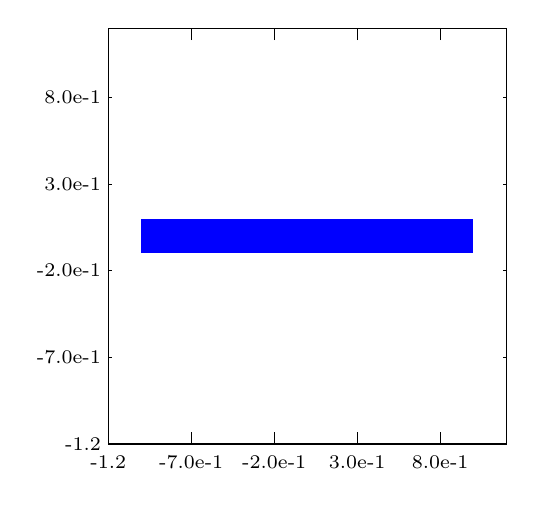
\begin{tikzpicture}[scale = 6,font=\scriptsize]
\draw (0.1148,0.085) rectangle (0.958,0.965);
\foreach \x/\label in {0.1148/-1.2,0.290466/-7.0e-1,0.466133/-2.0e-1,0.6418/3.0e-1,0.817466/8.0e-1} {
  \foreach \y in {0.94,0.085} \draw (\x,\y) -- (\x,\y+0.025);
  \node [below] at (\x,0.08) {\label};
}
\foreach \y/\label in {0.0849996/-1.2,0.268333/-7.0e-1,0.451666/-2.0e-1,0.635/3.0e-1,0.818333/8.0e-1} {
  \foreach \x in {0.951,0.1148} \draw (\x,\y) -- (\x+0.007,\y);
  \node [left] at (0.12,\y) {\label};
}
\fill [blue] (0.185067,0.488333) rectangle (0.887733,0.561667);
\end{tikzpicture}
\hspace{1cm}
% polygon
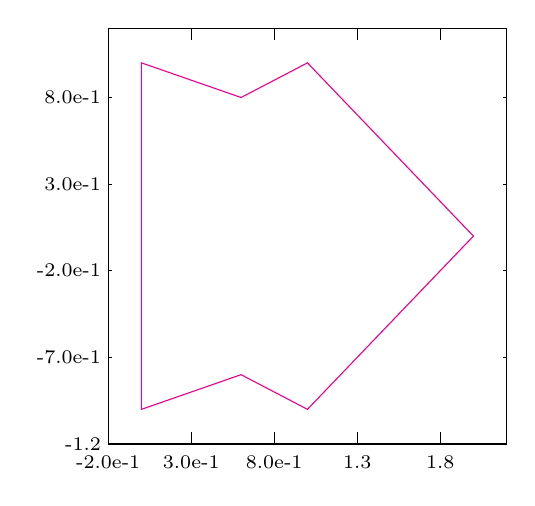
\begin{tikzpicture}[scale = 6,font=\scriptsize]
\draw (0.1148,0.085) rectangle (0.958,0.965);
\foreach \x/\label in {0.1148/-2.0e-1,0.290466/3.0e-1,0.466133/8.0e-1,0.6418/1.3,0.817466/1.8} {
  \foreach \y in {0.94,0.085} \draw (\x,\y) --(\x,\y+0.025);
  \node [below] at (\x,0.08) {\label};
}
\foreach \y/\label in {0.0849996/-1.2,0.268333/-7.0e-1,0.451666/-2.0e-1,0.635/3.0e-1,0.818333/8.0e-1} {
  \foreach \x in {0.951,0.1148} \draw (\x,\y) --(\x+0.007,\y);
  \node [left] at (0.12,\y) {\label};
}
\draw [magenta] (0.185067,0.891667) -- (0.185067,0.158333) -- (0.395867,0.231667) -- (0.5364,0.158333) -- (0.887733,0.525) -- (0.5364,0.891667) -- (0.395867,0.818333) -- cycle;
\end{tikzpicture}
\\[8mm]
% ellipse
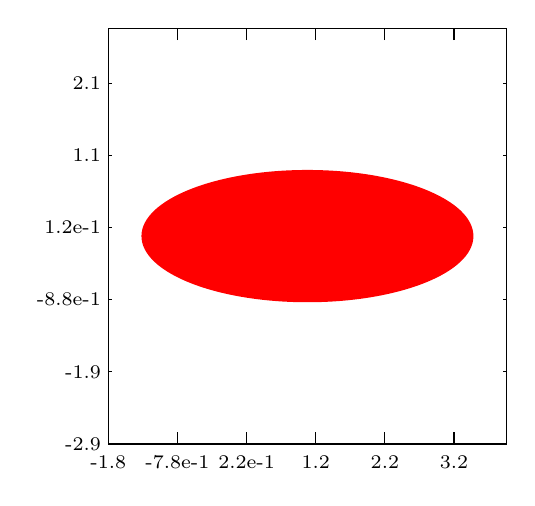
\begin{tikzpicture}[scale = 6,font=\scriptsize]
\draw (0.1148,0.085) rectangle (0.958,0.965);
\foreach \x/\label in {0.1148/-1.8,0.261189/-7.8e-1,0.407578/2.2e-1,0.553966/1.2,0.700355/2.2,0.846744/3.2} {
  \foreach \y in {0.94,0.085} \draw (\x,\y) --(\x,\y+0.025);
  \node [below] at (\x,0.08) {\label};
}
\foreach \y/\label in {0.0849996/-2.9,0.237777/-1.9,0.390555/-8.8e-1,0.543333/1.2e-1,0.696111/1.1,0.848888/2.1} {
  \foreach \x in {0.951,0.1148} \draw (\x,\y) --(\x+0.007,\y);
  \node [left] at (0.12,\y) {\label};
}
\fill [red] (0.5364,0.525) circle [x radius=0.351333,y radius=0.14];
\end{tikzpicture}
\hspace{1cm}
% ring
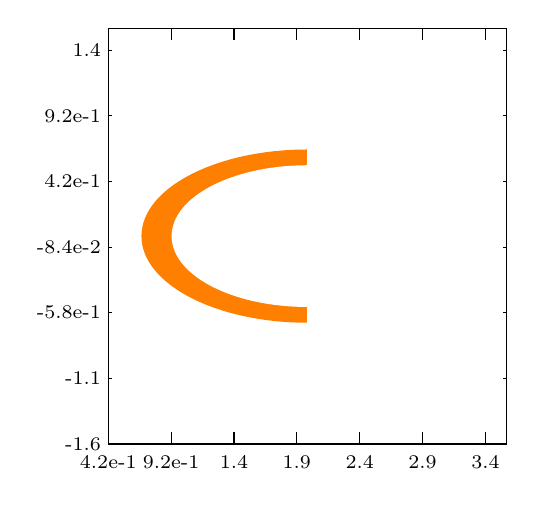
\begin{tikzpicture}[scale = 6,font=\scriptsize]
\draw (0.1148,0.085) rectangle (0.958,0.965);
\foreach \x/\label in {0.1148/4.2e-1,0.247881/9.2e-1,0.380962/1.4,0.514043/1.9,0.647123/2.4,0.780204/2.9,0.913285/3.4} {
  \foreach \y in {0.94,0.085} \draw (\x,\y) --(\x,\y+0.025);
  \node [below] at (\x,0.08) {\label};
}
\foreach \y/\label in {0.0849996/-1.6,0.223888/-1.1,0.362777/-5.8e-1,0.501666/-8.4e-2,0.640555/4.2e-1,0.779444/9.2e-1,0.918333/1.4} {
  \foreach \x in {0.951,0.1148} \draw (\x,\y) --(\x+0.007,\y);
  \node [left] at (0.12,\y) {\label};
}
\fill [color=orange] (0.5364,0.525) circle [x radius=0.351333,y radius=0.183333];
\fill [color=white] (0.5364,0.525) circle [x radius=0.287455,y radius=0.15];
\fill [color=white] (0.5364,0.158333) rectangle (0.9,0.784272);
\end{tikzpicture}
\caption{\label{fig:rg}Sample regions defined via the \ident{RG} class: interval (top left), polygon (top right), ellipse (bottom left), and ring (bottom right). These plots can be generated at run time by adding the command-line option \texttt{-rg\_view draw}.}
\end{figure}

Sometimes it is useful to specify the complement of a certain region, e.g., the part of the complex plane outside an ellipse. This can be achieved with
        \findex{RGSetComplement}
        \begin{Verbatim}[fontsize=\small]
        RGSetComplement(RG rg,PetscBool flg)
        \end{Verbatim}
or in the command line with \Verb!-rg_complement!.

By default, a newly created \ident{RG} object that is not set a type nor parameters must represent the whole complex plane (the same as \texttt{RGINTERVAL} with values $[-\infty,+\infty]\times[-\infty,+\infty]$). We call this the \emph{trivial} region, and provide a function to test this situation:
        \findex{RGIsTrivial}
        \begin{Verbatim}[fontsize=\small]
        RGIsTrivial(RG rg,PetscBool *trivial)
        \end{Verbatim}

Another useful operation is to check whether a given point of the complex plane is inside the region or not:
        \findex{RGCheckInside}
        \begin{Verbatim}[fontsize=\small]
        RGCheckInside(RG rg,PetscInt n,PetscScalar *ar,PetscScalar *ai,PetscInt *inside)
        \end{Verbatim}
Note that the point is represented as two \texttt{PetscScalar}'s, similarly to eigenvalues in \slepc.

\begin{table}
\centering
{\small \begin{tabular}{lll}
                       &                     & {\footnotesize Options} \\
Region Type            & \ident{RGType}      & {\footnotesize Database Name}\\\hline
(Generalized) Interval & \texttt{RGINTERVAL} & \texttt{interval} \\
Polygon                & \texttt{RGPOLYGON}  & \texttt{polygon} \\
Ellipse                & \texttt{RGELLIPSE}  & \texttt{ellipse} \\
Ring                   & \texttt{RGRING}     & \texttt{ring} \\\hline
\end{tabular} }
\caption{\label{tab:rg}Regions available as \ident{RG} objects.}
\end{table}

%---------------------------------------------------
\section{Directory Structure}

The directory structure of the \slepc software is very similar to that in \petsc. The root directory of \slepc contains the following directories:
\begin{description}
\item[\texttt{lib/slepc/conf}] - Directory containing the base \slepc makefile, to be included in application makefiles.
\item[\texttt{config}] - \slepc configuration scripts.
\item[\texttt{docs}] - All documentation for \slepc, including this manual. The subdirectory \texttt{manualpages} contains the on-line manual pages of each \slepc routine.
\item[\texttt{include}] - All include files for \slepc. The following subdirectories exist:
\begin{description}
\setlength{\itemsep}{0mm}
\item[\texttt{slepc/finclude}] - include files for Fortran programmers.
\item[\texttt{slepc/private}] - include files containing implementation details, for developer use only.
\end{description}
\item[\texttt{share/slepc}] - Common files, including:
\begin{description}
\setlength{\itemsep}{0mm}
\item[\texttt{datafiles}] - data files used by some examples.
%\item[\texttt{matlab}] - Matlab interface and examples.
\end{description}
\item[\texttt{src}] - The source code for all \slepc components, which currently includes:
\begin{description}
\setlength{\itemsep}{0mm}
\item[\texttt{sys}] - system-related routines and auxiliary classes \texttt{bv}, \texttt{ds}, \texttt{fn}, \texttt{rg}, \texttt{st}.
\item[\texttt{eps}] - eigenvalue problem solver.
\item[\texttt{svd}] - singular value decomposition solver.
\item[\texttt{pep}] - polynomial eigenvalue problem solver.
\item[\texttt{nep}] - nonlinear eigenvalue problem solver.
\item[\texttt{mfn}] - matrix function.
\item[\texttt{lme}] - linear matrix equations.
\end{description}
\item[\texttt{\$PETSC\_ARCH}] - For each value of \ident{PETSC\_ARCH}, a directory exists containing files generated during installation of that particular configuration. The following subdirectories exist:
\begin{description}
\setlength{\itemsep}{0mm}
\item[\texttt{lib}] - all the generated libraries.
\item[\texttt{lib/slepc/conf}] - configuration parameters and log files.
\item[\texttt{include}] - automatically generated include files, such as Fortran 90 \texttt{*.mod} files.
\end{description}
\end{description}

Each \slepc source code component directory has the following subdirectories:
\begin{description}
\item[\texttt{interface}] - The calling sequences for the abstract interface to the components. Code here does not know about particular implementations.
\item[\texttt{impls}] - Source code for the different implementations.
\item[\texttt{tutorials}] - Example programs intended for learning to use \slepc.
\item[\texttt{tests}] - Example programs used by testing scripts.
\end{description}

%---------------------------------------------------
%\section{Auxiliary Components}
%\label{sec:aux}

%The previous section includes a list of subdirectories, each of them representing a \slepc component. Most of these components have been treated in previous chapters. Here we include a brief report about two auxiliary components, \ident{BV} and \ident{DS}, that are not normally required by final users, but provide important operations to high level solvers such \ident{EPS}.

%\subsection{BV: Basis Vectors}

%\subsection{DS: Direct Solver (or Dense System)}

%---------------------------------------------------
\section{Wrappers to External Libraries}
\label{sec:wrap}

\slepc interfaces to several external libraries for the solution of eigenvalue problems. This section provides a short description of each of these packages as well as some hints for using them with \slepc, including pointers to the respective websites from which the software can be downloaded. The description may also include method-specific parameters, that can be set in the same way as other \slepc options, either procedurally or via the command-line.

In order to use \slepc together with an external library such as \arpack, one needs to do the following.
\begin{enumerate}
\item Install the external software, with the same compilers and MPI that will be used for \petsc/\slepc.
\item Enable the utilization of the external software from \slepc by specifying configure options as explained in \S\ref{sec:opt-inst}.
 \item Build the \slepc libraries.
\item Use the runtime option \Verb!-eps_type <type>! to select the solver.
\end{enumerate}

Exceptions to the above rule are \lapack, which should be enabled during \petsc's configuration, and \blopex, that must be installed with \Verb!--download-blopex! in \slepc's configure. Other packages also support the download option.

\subsection*{\underline{\lapack}}
\begin{description}
\setlength{\itemsep}{0pt}
\item[References.]\citep{Anderson:1999:LUG}.
\item[Website.] \url{https://www.netlib.org/lapack}.
\item[Version.] 3.0 or later.
\item[Summary.] \lapack\ (Linear Algebra PACKage) is a software package for the solution of many different dense linear algebra problems, including various types of eigenvalue problems and singular value decompositions.

\slepc explicitly creates the operator matrix in dense form and then the appropriate \lapack driver routine is invoked. Therefore, this interface should be used only for testing and validation purposes and not in a production code. The operator matrix is created by applying the operator to the columns of the identity matrix.

\item[Installation.]
The \slepc interface to \lapack can be used directly. If \slepc's configure script complains about missing \lapack functions, then configure \petsc with option \texttt{-{}-download-f2cblaslapack}.
\end{description}

\subsection*{\underline{\arpack}}
\begin{description}
\setlength{\itemsep}{0pt}
\item[References.]\citep{Lehoucq:1998:AUG}, \citep{Maschhoff:1996:PEP}.
\item[Website.] \url{https://github.com/opencollab/arpack-ng}.
\item[Version.] Release 2 (plus patches).
\item[Summary.] \arpack\ (ARnoldi PACKage) is a software package for the computation of a few eigenvalues and corresponding eigenvectors of a general $n\times n$ matrix $A$. It is most appropriate for large sparse or structured matrices, where structured means that a matrix-vector product $w \leftarrow Av$ requires order $n$ rather than the usual order $n^2$ floating point operations.

\arpack\ is based upon an algorithmic variant of the Arnoldi process called the Implicitly Restarted Arnoldi Method (IRAM). When the matrix $A$ is symmetric it reduces to a variant of the Lanczos process called the Implicitly Restarted Lanczos Method (IRLM). These variants may be viewed as a synthesis of the Arnoldi/Lanczos process with the Implicitly Shifted QR technique that is suitable for large scale problems.

It can be used for standard and generalized eigenvalue problems, both in real and complex arithmetic. It is implemented in Fortran 77 and it is based on the reverse communication interface. A parallel version, \parpack, is available with support for both MPI and BLACS.
\item[Installation.]
To install from the original website: first of all, unpack \texttt{arpack96.tar.gz} and also the patch file \texttt{patch.tar.gz}. If you plan to use the parallel version, extract also the contents of the file \texttt{parpack96.tar.gz} together with the patches \texttt{ppatch.tar.gz} (make sure you delete any \texttt{mpif.h} files that could exist in the directory tree). After setting all the directories, modify the \texttt{ARmake.inc} file and then compile the software with \texttt{make all}. It is recommended that \arpack is installed with its own \lapack version since it may give unexpected results with more recent versions of \lapack.

Alternatively, one can use the \textsc{arpack-ng} distribution, available in \texttt{github.com}, that supports \texttt{configure}+\texttt{make} for installation. Also, \slepc's \texttt{configure} allows to download this version automatically via the \texttt{-{}-download-arpack} option.

It is possible to configure \slepc with the serial version of \arpack. For this, you have to configure \petsc with the option \texttt{-{}-with-mpi=0}.
\end{description}

\subsection*{\underline{\primme}}
\begin{description}
\setlength{\itemsep}{0pt}
\item[References.]\citep{Stathopoulos:2010:PMS}.
\item[Website.] \url{https://www.cs.wm.edu/~andreas/software}.
\item[Version.] 3.2.
\item[Summary.] \primme (PReconditioned Iterative MultiMethod Eigensolver) is a C library for finding a number of eigenvalues and their corresponding eigenvectors of a real symmetric (or complex Hermitian) matrix. This library provides a multimethod eigensolver, based on Davidson/Jacobi-Davidson. Particular methods include GD+1, JDQMR, and LOBPCG. It supports preconditioning as well as the computation of interior eigenvalues.
\item[Installation.] Type \texttt{make lib} after customizing the file \texttt{Make\_flags} appropriately. Alternatively, the \texttt{-{}-download-primme} option is also available in \slepc's \texttt{configure}.
\item[Specific options.] Since PRIMME contains preconditioned solvers, the \slepc interface uses \ident{STPRECOND}, as described in \ref{sec:precond}.

The \slepc interface to this package allows the user to specify the maximum allowed block size with the function \ident{EPSPRIMMESetBlockSize} or at run time with the option \Verb!-eps_primme_blocksize <size>!.
For changing the particular algorithm within \primme, use the function \ident{EPSPRIMMESetMethod}.

\primme also provides a solver for the singular value decomposition that is interfaced in \slepc's \ident{SVD}, see chapter \ref{cap:svd}.
\end{description}

\subsection*{\underline{\evsl}}
\begin{description}
\setlength{\itemsep}{0pt}
\item[References.]\citep{Li:2019:EVS}.
\item[Website.] \url{https://www-users.cs.umn.edu/~saad/software/EVSL/}.
\item[Summary.] \evsl is a sequential library that implements methods for computing all eigenvalues located in a given interval for real symmetric (standard or generalized) eigenvalue problems. Currently SLEPc only supports standard problems.
\item[Installation.] The option \texttt{-{}-download-evsl} is available in \slepc's configure for easy installation. Alternatively, one can use an already installed version.
\end{description}

\subsection*{\underline{\trlan}}
\begin{description}
\setlength{\itemsep}{0pt}
\item[References.]\citep{Wu:2000:TLM}.
\item[Website.] \url{https://sdm.lbl.gov/\~kewu/trlan.html}.
\item[Version.] 201009.
\item[Summary.] This package provides a Fortran 90 implementation of the dynamic thick-restart Lanczos algorithm. This is a specialized version of Lanczos that targets only the case in which one wants both eigenvalues and eigenvectors of a large real symmetric eigenvalue problem that cannot use the shift-and-invert scheme. In this case the standard non-restarted Lanczos algorithm requires to store a large number of Lanczos vectors, what can cause storage problems and make each iteration of the method very expensive.

\trlan{} requires the user to provide a matrix-vector multiplication routine. The parallel version uses MPI as the message passing layer.
\item[Installation.] To install this package, it is necessary to have access to a Fortran 90 compiler. The compiler name and the options used are specified in the file called \texttt{Make.inc}. To generate the library, type \texttt{make plib} in the \texttt{TRLan} directory. Alternatively, the \texttt{-{}-download-trlan} option is also available in \slepc's \texttt{configure}.

It is possible to configure \slepc with the serial version of \trlan (built with \texttt{make lib}). For this, you have to configure \petsc with the option \texttt{-{}-with-mpi=0}.
\end{description}

\subsection*{\underline{\blopex}}
\begin{description}
\setlength{\itemsep}{0pt}
\item[References.]\citep{Knyazev:2007:BLO}.
\item[Website.] \url{https://github.com/lobpcg/blopex}.
\item[Summary.] \blopex is a package that implements the Locally Optimal Block Preconditioned Conjugate Gradient (LOBPCG) method for computing several extreme eigenpairs of symmetric positive generalized eigenproblems. Numerical comparisons suggest that this method is a genuine analog for eigenproblems of the standard preconditioned conjugate gradient method for symmetric linear systems.
\item[Installation.] In order to use \blopex from \slepc, it necessary to install it during \slepc's configuration: \Verb!./configure --download-blopex!.
\item[Specific options.] Since BLOPEX contains preconditioned solvers, the \slepc interface uses \ident{STPRECOND}, as described in \ref{sec:precond}.
\end{description}

\subsection*{\underline{\scalapack}}
\begin{description}
\setlength{\itemsep}{0pt}
\item[References.]\citep{Blackford:1997:SUG}.
\item[Website.] \url{https://www.netlib.org/scalapack}.
\item[Summary.] \scalapack is a library of high-performance linear algebra routines for parallel distributed memory machines. It contains eigensolvers for dense Hermitian eigenvalue problems, as well as solvers for the (dense) SVD.
\item[Installation.] For using \scalapack from \slepc it is necessary to select it during configuration of \petsc.
\end{description}

\subsection*{\underline{\elpa}}
\begin{description}
\setlength{\itemsep}{0pt}
\item[References.]\citep{Auckenthaler:2011:ELP}.
\item[Website.] \url{https://elpa.mpcdf.mpg.de/}.
\item[Summary.] \elpa is a high-performance library for the parallel solution of dense symmetric (or Hermitian) eigenvalue problems on distributed memory computers. It uses a ScaLAPACK-compatible matrix distribution.
\item[Installation.] The \slepc wrapper to \elpa can be activated at configure time with the option \texttt{-{}-download\_elpa}, in which case \scalapack support must have been enabled during the configuration of \petsc.
\end{description}

\subsection*{\underline{\ksvd}}
\begin{description}
\setlength{\itemsep}{0pt}
\item[References.]\citep{Sukkari:2019:QDW}.
\item[Website.] \url{https://github.com/ecrc/ksvd/}.
\item[Summary.] \ksvd is a high performance software framework for computing a dense SVD on distributed-memory manycore systems. The \ksvd solver relies on the polar decomposition (PD) based on the QR Dynamically-Weighted Halley (QDWH) and ZOLO-PD algorithms.
\item[Installation.] The option \texttt{-{}-download-ksvd} is available in \slepc's configure for easy installation, which in turn requires adding \texttt{-{}-download-polar} and \texttt{-{}-download-elpa}.
\end{description}

\subsection*{\underline{\elemental}}
\begin{description}
\setlength{\itemsep}{0pt}
\item[References.]\citep{Poulson:2013:ELE}.
\item[Website.] \url{https://github.com/elemental/Elemental}.
\item[Summary.] \elemental is distributed-memory, arbitrary-precision, dense and sparse-direct linear algebra package. It contains eigensolvers for dense Hermitian eigenvalue problems, as well as solvers for the SVD.
\item[Installation.] For using \elemental from \slepc it is necessary to select it during configuration of \petsc.
\end{description}

\subsection*{\underline{\feast}}
\begin{description}
\setlength{\itemsep}{0pt}
\item[References.]\citep{Polizzi:2009:DAS}.
\item[Website.] \url{https://feast-solver.org/}.
\item[Summary.] \feast is a numerical library for solving the standard or generalized symmetric eigenvalue problem, and obtaining all the eigenvalues and eigenvectors within a given search interval. It is based on an innovative fast and stable numerical algorithm which deviates fundamentally from the traditional Krylov subspace based iterations or Davidson-Jacobi techniques. The FEAST algorithm takes its inspiration from the density-matrix representation and contour integration technique in quantum mechanics. Latest versions also support non-symmetric problems.
\item[Installation.] We only support the \feast implementation included in Intel MKL. For using it from \slepc it is necessary to configure \petsc with MKL by adding the corresponding option, e.g., \Verb!--with-blas-lapack-dir=$MKLROOT!.
\item[Specific options.] The \slepc interface to \feast allows the user to specify the number of contour integration points with the function \ident{EPSFEASTSetNumPoints} or at run time with the option \Verb!-eps_feast_num_points <n>!.
\end{description}

\subsection*{\underline{\chase}}
\begin{description}
\setlength{\itemsep}{0pt}
\item[References.]\citep{Winkelmann:2019:CCA}.
\item[Website.] \url{https://github.com/ChASE-library/ChASE}.
\item[Summary.] \chase is a modern and scalable library based on subspace iteration with polynomial acceleration to solve dense Hermitian (symmetric) algebraic eigenvalue problems, especially solving dense Hermitian eigenproblems arranged in a sequence. Novel to ChASE is the computation of the spectral estimates that enter in the filter and an optimization of the polynomial degree that further reduces the necessary floating-point operations.
\item[Installation.] Currently, the \chase interface in \slepc is based on the MPI version with block-cyclic distribution, i.e., \scalapack matrix storage, so it is necessary to enable \scalapack during configuration of \petsc.
\end{description}

%---------------------------------------------------
\section{Fortran Interface}
\label{sec:fortran}

\slepc provides an interface for Fortran programmers, very much like \petsc. As in the case of \petsc, there are slight differences between the C and Fortran \slepc interfaces, due to differences in Fortran syntax. For instance, the error checking variable is the final argument of all the routines in the Fortran interface, in contrast to the C convention of providing the error variable as the routine's return value.

The following is a Fortran example. It is the Fortran equivalent of the program given in \S\ref{sec:simpleex} and can be found in \Verb!${SLEPC_DIR}/src/eps/tutorials! (file \texttt{ex1f.F90}).
\MyVerbatimInput{ex1f.F90}

%---------------------------------------------------
%\section{Matlab Interface}
%\label{sec:matlab}
%
%Since version 3.2, \slepc includes an interface intended to make most of \slepc's functionality available from Matlab. It is experimental and needs further development, so users planning to use it seriously are recommended to contact the authors. Below are some guidelines for using this interface.
%
%First of all, \petsc must have been configured with the Matlab interface enabled. This can be done as follows (check \petsc documentation for details):
%       \begin{Verbatim}[fontsize=\small]
%       $ ./configure --with-matlab --with-matlab-engine --with-shared-libraries
%       \end{Verbatim}
%
%Once the \petsc and \slepc libraries have been built, one has to set Matlab's path to point to the directories containing Matlab classes: \Verb!$SLEPC_DIR/share/slepc/matlab/classes! and \Verb!$PETSC_DIR/share/slepc/matlab/classes!. Below we show a simple Matlab example (included in \slepc's distribution) that does this, and then solves a simple eigenproblem.
%\MyVerbatimInput{exEPS.m}



%---------------------------------------------------
\cleardoublepage
\fancyhead{}\fancyhead[LO,RE]{\nouppercase{\scriptsize \sffamily Bibliography}}
\addcontentsline{toc}{chapter}{Bibliography}

%\bibliographystyle{engnat}
%\bibliography{slepc}
%-------------------------------------------------------
% SLEPc Users Manual
%-------------------------------------------------------

\documentclass[titlepage,10pt,a4paper]{book}

\usepackage{xcolor}
\usepackage{graphicx}
\usepackage[square]{natbib}
\usepackage{fancyhdr}
\usepackage{fancyvrb}
\usepackage{caption}
\usepackage{xspace}
\usepackage{ae,aecompl}
\usepackage{amsmath,amssymb}
\usepackage{imakeidx}
\usepackage{hyperref}
\usepackage{titlesec}
\usepackage{tikz,pgfplots}

\makeindex

\hypersetup{
  colorlinks,
  linkcolor=purple,
  citecolor=violet,
  filecolor=blue,
  urlcolor=magenta,
  bookmarksnumbered,
  pdfstartview=FitH,
  pdftitle={SLEPc Users Manual},
  pdfauthor={J. E. Roman, C. Campos, L. Dalcin, E. Romero, A. Tomas},
  pdfsubject={SLEPc: Scalable Library for Eigenvalue Problem Computations},
  pdfkeywords={SLEPc, PETSc, eigenvalue problems}
}

\newcommand{\slepcversion}{3.23}
\newcommand{\slepchome}{https://slepc.upv.es}
\newcommand{\pack}[1]{{\sc #1}\index{\textsc{#1}}\xspace}
\newcommand{\packnoi}[1]{{\sc #1}\xspace}
\newcommand{\slepc}{\texorpdfstring{\packnoi{slep\rm c}}{{SLEPc}}}
\newcommand{\petsc}{\pack{pets\rm c}}
\newcommand{\blas}{\pack{blas}}
\newcommand{\lapack}{\pack{lapack}}
\newcommand{\arpack}{\pack{arpack}}
\newcommand{\parpack}{\pack{parpack}}
\newcommand{\trlan}{\pack{trlan}}
\newcommand{\primme}{\pack{primme}}
\newcommand{\blopex}{\pack{blopex}}
\newcommand{\scalapack}{\pack{scalapack}}
\newcommand{\elpa}{\pack{elpa}}
\newcommand{\elemental}{\pack{elemental}}
\newcommand{\evsl}{\pack{evsl}}
\newcommand{\feast}{\pack{feast}}
\newcommand{\ksvd}{\pack{ksvd}}
\newcommand{\chase}{\pack{chase}}
\newcommand{\mpich}{\pack{mpich}}
\newcommand{\expokit}{\pack{expokit}}
\newcommand{\rutina}[1]{\texttt{#1}\index{\texttt{#1}}}
\newcommand{\ident}[1]{\texttt{#1}\index{\texttt{#1}}}
\newcommand{\findex}[1]{\index{\texttt{#1}}}

\DeclareMathOperator{\rev}{rev}

%VerbatimEnvironment%
\fvset{numbers=left,numbersep=6pt,stepnumber=5}
\newcommand{\MyVerbatimInput}[1]{\fvset{fontsize=\scriptsize}%
  \VerbatimInput{#1}%
  \fvset{fontsize=\normalsize}%
}

\setlength{\textwidth}{14.5cm}
\setlength{\tabcolsep}{2mm}
\renewcommand{\arraystretch}{1.05}
\setcounter{tocdepth}{3}
\renewcommand{\captionlabelfont}{\sl\sffamily}
\makeatletter\@ifundefined{bibfont}{\newcommand{\bibfont}{\small}}{\renewcommand{\bibfont}{\small}}\makeatother

\titleformat{\chapter}[display]
  {\bfseries\Large}
  {\filleft\setlength{\fboxsep}{2mm}\fbox{\large\sc\chaptertitlename}\hspace*{-0.5mm}\setlength{\fboxsep}{4mm}\setlength{\fboxrule}{.5mm}\fbox{\Huge\bfseries\thechapter}}
  {4ex}
  {\huge\bf\sffamily
   \filright}
  [\hfill\rule{10cm}{1pt}]

\begin{document}

\title{
   \vspace*{-1cm}
   \framebox[12cm][l]{
   \includegraphics[height=1.4cm]{figures/upv}
   \hfill
   \parbox[b]{4cm}{\begin{flushright}\vspace*{-7mm}\normalsize\sl\sffamily
   Departamento de\\[-0.8mm] Sistemas Inform\'aticos\\[-0.8mm]
   y Computaci\'on\\[0.8mm]
   \vspace{-2.5mm}\end{flushright}}
   \raisebox{3mm}{\includegraphics[height=9mm,width=1.4cm]{figures/dsic}}
   }
   \\[2cm]
   \normalsize Technical Report DSIC-II/24/02
   \\[2cm]
   \vspace*{6mm}
   {\Large\bf\sffamily
   SLEPc Users Manual\\[2mm]}
   {\large\bf\sffamily
   Scalable Library for Eigenvalue Problem Computations}\\[2mm]
   \vspace*{6mm}
   \vspace*{6mm}
   \url{\slepchome}
   \\[6mm]
}

\author{
  Jose E. Roman\\
  Carmen Campos\\
  Lisandro Dalcin\\
  Eloy Romero\\
  Andr\'es Tom\'as\\[3mm]
}

\date{
   To be used with \slepc \slepcversion\\
   March, 2025
}

\hypersetup{pageanchor=false}
\begin{titlepage}
\maketitle
\end{titlepage}

\setlength{\textheight}{18cm}
\setlength{\oddsidemargin}{0.6cm}
\setlength{\evensidemargin}{0.6cm}
\setlength{\footskip}{2cm}
\setlength{\voffset}{1.3cm}

\pagestyle{empty}
\cleardoublepage
\hypersetup{pageanchor=true}

{
  \pagestyle{plain}
  \pagenumbering{roman}
%---------------------------------------------------
\subsection*{Abstract}

This document describes \slepc, the {\em Scalable Library for Eigenvalue Problem Computations}, a software package for the solution of large sparse eigenproblems on parallel computers. It can be used for the solution of various types of eigenvalue problems, including linear and nonlinear, as well as other related problems such as the singular value decomposition (see a summary of supported problem classes on page \pageref{tab:modules}). \slepc is a general library in the sense that it covers both Hermitian and non-Hermitian problems, with either real or complex arithmetic.

The emphasis of the software is on methods and techniques appropriate for problems in which the associated matrices are large and sparse, for example, those arising after the discretization of partial differential equations. Thus, most of the methods offered by the library are projection methods, including different variants of Krylov and Davidson iterations. In addition to its own solvers, \slepc provides transparent access to some external software packages such as \packnoi{arpack}. These packages are optional and their installation is not required to use \slepc, see \S\ref{sec:wrap} for details. Apart from the solvers, \slepc also provides built-in support for some operations commonly used in the context of eigenvalue computations, such as preconditioning or the shift-and-invert spectral transformation.

\slepc is built on top of \packnoi{pets\rm c}, the Portable, Extensible Toolkit for Scientific Computation \citep{Balay:PUM}. It can be considered an extension of \packnoi{pets\rm c} providing all the functionality necessary for the solution of eigenvalue problems. This means that \packnoi{pets\rm c} must be previously installed in order to use \slepc. \packnoi{pets\rm c} users will find \slepc very easy to use, since it enforces the same programming paradigm. Those readers that are not acquainted with \packnoi{pets\rm c} are highly recommended to familiarize with it before proceeding with \slepc.


\subsubsection*{How to Get \slepc}

All the information related to \slepc can be found at the following web site:
\begin{quote}
\begin{center}
\url{\slepchome}.
\end{center}
\end{quote}
The distribution file is available for download at this site. Other information is provided there, such as installation instructions and contact information. Instructions for installing the software can also be found in \S\ref{sec:inst}.

\packnoi{pets\rm c} can be downloaded from \url{https://petsc.org}.  \packnoi{pets\rm c} is supported, and information on contacting support can be found at that site.

\subsubsection*{Additional Documentation}

This manual provides a general description of \slepc. In addition, manual pages for individual routines are included in the distribution file in hypertext format, and are also available on-line at \url{\slepchome/documentation}. These manual pages provide hyperlinked access to the source code and enable easy movement among related topics. Finally, there are also several hands-on exercises available, which are intended for learning the basic concepts easily.

\subsubsection*{How to Read this Manual}

Users that are already familiar with \packnoi{pets\rm c} can read chapter \ref{cap:int} very fast. Section \ref{sec:eig} provides a brief overview of eigenproblems and the general concepts used by eigensolvers, so it can be skipped by experienced users. Chapters \ref{cap:eps}--\ref{cap:mfn} describe the main \slepc functionality. Some of them include an advanced usage section that can be skipped at a first reading. Finally, chapter \ref{cap:add} contains less important, additional information.

%\subsubsection*{What's New}
%
%The major changes in the Users Manual with respect to the previous version are:
%\begin{itemize}
%\setlength{\itemsep}{-2pt}
%\item New section \S\ref{sec:gsvd} related to the generalized singular value decomposition (GSVD). The rest of Ch.~\ref{cap:svd} has been slightly modified to cover the new GSVD functionality.
%\end{itemize}

\subsubsection*{\slepc Technical Reports}

The information contained in this manual is complemented by a set of Technical Reports, which provide technical details that normal users typically do not need to know but may be useful for experts in order to identify the particular method implemented in \slepc. These reports are not included in the \slepc distribution file but can be accessed via the \slepc web site. A \hyperlink{str}{list of available reports} is included at the end of the Bibliography.


\subsubsection*{Acknowledgments}

%We thank all the \packnoi{pets\rm c} team for their help and support. Without their continued effort invested in \packnoi{pets\rm c}, \slepc would not have been possible.
% We also thank Osni Marques and Tony Drummond for helping us raise awareness of \slepc in the context of the ACTS project.

The current version contains code contributed by:
A.\ Lamas Davi\~{n}a (CUDA code),
F.\ Alvarruiz (restarted Lanczos for the GSVD, structured BSE solvers),
B.\ Mellado-Pinto (structured BSE solvers),
Y.\ Maeda, T.\ Sakurai (CISS solvers),
M.\ Moldaschl, W.\ Gansterer (BDC subroutines),
F.\ Kong (nonlinear inverse iteration),
H.\ Fang, Y. Saad (\textsc{filtlan} polynomial filter).

Development of \slepc has been partially funded by the following grants:
\begin{itemize}
\setlength{\itemsep}{-2pt}
\item Innovation Study ISOLV-BSE has received funding through the Inno4scale project, which is funded by the European High-Performance Computing Joint Undertaking (JU) under Grant Agreement No 101118139. The JU receives support from the European Union's Horizon Europe Programme.
\item Agencia Estatal de Investigaci\'on (Spain), grant no.\ PID2022-139568NB-I00, PI: Jos\'e E. Rom\'an.
\item Agencia Estatal de Investigaci\'on (Spain), grant no.\ PID2019-107379RB-I00, PI: Jos\'e E. Rom\'an.
\item Agencia Estatal de Investigaci\'on (Spain), grant no.\ TIN2016-75985-P, PI: Jos\'e E. Rom\'an.
\item Ministerio de Econom\'{\i}a y Comp.\ (Spain), grant no.\ TIN2013-41049-P, PI: Jos\'e E. Rom\'an.
\item Ministerio de Ciencia e Innovaci\'on (Spain), grant no.\ TIN2009-07519, PI: Jos\'e E. Rom\'an.
\item Valencian Regional Government, grant no.\ GV06/091, PI: Jos\'e E. Rom\'an.
\item Valencian Regional Government, grant no.\ CTIDB/2002/54, PI: Vicente Hern\'andez.
\end{itemize}

\subsubsection*{License and Copyright}

Starting from version 3.8, \slepc is released under a 2-clause BSD license (see \texttt{LICENSE} file).

\begin{quote}
\begin{sffamily}
Copyright 2002--2025 Universitat Polit\`ecnica de Valencia, Spain
\end{sffamily}
\end{quote}

%---------------------------------------------------
\newpage
\subsubsection*{Supported Problem Classes}

The following table provides an overview of the functionality offered by \slepc, organized by problem classes.

\begin{table}[h]
\label{tab:modules}
\centering
{\small \begin{tabular}{lccc}
Problem class                 & Model equation  & Module       & Chapter \\\hline
Linear eigenvalue problem     & $Ax=\lambda x,\quad Ax=\lambda Bx$ & \texttt{EPS} & \ref{cap:eps} \\
Quadratic eigenvalue problem  & $(K+\lambda C+\lambda^2M)x=0$ & -- & -- \\
Polynomial eigenvalue problem & $(A_0+\lambda A_1+\cdots+\lambda^dA_d)x=0$ & \texttt{PEP} & \ref{cap:pep} \\
Nonlinear eigenvalue problem  & $T(\lambda)x=0$ & \texttt{NEP} & \ref{cap:nep} \\\hline
Singular value decomposition  & $Av=\sigma u$   & \texttt{SVD} & \ref{cap:svd} \\
Matrix function (action of)   & $y=f(A)v$   & \texttt{MFN} & \ref{cap:mfn} \\
Linear matrix equation        & $AXE+DXB=C$   & \texttt{LME} & See notes \\\hline
\end{tabular} }
\end{table}

\noindent In order to solve a given problem, one should create a solver object corresponding to the solver class (module) that better fits the problem (the less general one; e.g., we do not recommend using \texttt{NEP} to solve a linear eigenproblem).\\[3mm]

\noindent Notes:\vspace{-2mm}
\begin{itemize}
\setlength{\itemsep}{-2pt}
\item Most users are typically interested in linear eigenproblems only.
\item In each problem class there may exist several subclasses (problem types in \slepc terminology), for instance symmetric-definite generalized eigenproblem in \texttt{EPS}.
\item The solver class (module) is named after the problem class. For historical reasons, the one for linear eigenvalue problems is called \texttt{EPS} rather than \texttt{LEP}.
\item In addition to the SVD shown in the table, the \texttt{SVD} module also supports other related problems such as the GSVD and the HSVD.
\item In previous \slepc versions there was a \texttt{QEP} module for quadratic eigenproblems. It has been replaced by \texttt{PEP}. %See \S\ref{sec:qeppep} for upgrading application code that used \texttt{QEP}.
\item For the action of a matrix function (\texttt{MFN}), in \slepc we focus on methods that are closely related to methods for eigenvalue problems.
\item The solver class \texttt{LME} is still experimental and it is not covered in this manual yet.
\end{itemize}

%---------------------------------------------------
  \setlength{\parskip}{0cm}
  \tableofcontents
}
\cleardoublepage
\pagenumbering{arabic}
\pagestyle{fancy}
\renewcommand{\chaptermark}[1]{\markboth{\scriptsize \sffamily {\bfseries\chaptername\ \thechapter.} #1}{}}
\renewcommand{\sectionmark}[1]{\markright{\scriptsize \sffamily {\bfseries\thesection.} #1}{}}
\fancyhead{}
\fancyhead[LE,RO]{\nouppercase{\rightmark}}
\fancyhead[LO,RE]{\nouppercase{\leftmark}}
\fancyfoot[C]{\scriptsize --- \thepage\ ---}
\renewcommand{\headrulewidth}{0.2pt}
\renewcommand{\footrulewidth}{0.2pt}

%-------------------------------------------------------
% SLEPc Users Manual
%-------------------------------------------------------
\chapter{\label{cap:int}Getting Started}
%-------------------------------------------------------

\noindent \slepc, the {\em Scalable Library for Eigenvalue Problem Computations}, is a software library for the solution of large sparse eigenvalue problems on parallel computers.

Together with linear systems of equations, eigenvalue problems are a very important class of linear algebra problems. The need for the numerical solution of these problems arises in many situations in science and engineering, in problems associated with stability and vibration analysis in practical applications. These are usually formulated as large sparse eigenproblems.

Computing eigenvalues is essentially more difficult than solving linear systems of equations. This has resulted in a very active research activity in the area of computational methods for eigenvalue problems in the last years, with many remarkable achievements.  However, these state-of-the-art methods and algorithms are not easily transferred to the scientific community, and, apart from a few exceptions, most user still rely on simpler, well-established techniques.

The reasons for this situation are diverse. First, new methods are increasingly complex and difficult to implement and therefore robust implementations must be provided by computational specialists, for example as software libraries. The development of such libraries requires to invest a lot of effort but sometimes they do not reach normal users due to a lack of awareness.

In the case of eigenproblems, using libraries is not straightforward. It is usually recommended that the user understands how the underlying algorithm works and typically the problem is successfully solved only after several cycles of testing and parameter tuning. Methods are often specific for a certain class of eigenproblems and this leads to an explosion of available algorithms from which the user has to choose. Not all these algorithms are available in the form of software libraries, even less frequently with parallel capabilities.

Another difficulty resides in how to represent the operator matrix. Unlike in dense methods, there is no widely accepted standard for basic sparse operations in the spirit of \blas. This is due to the fact that sparse storage is more complicated, admitting of more variation, and therefore less standardized. For this reason, sparse libraries have an added level of complexity. This holds even more so in the case of parallel distributed-memory programming, where the data of the problem have to be distributed across the available processors.

The first implementations of algorithms for sparse matrices required a prescribed storage format for the sparse matrix, which is an obvious limitation. An alternative way of matrix representation is by means of a user-provided subroutine for the matrix-vector product. Apart from being format-independent, this approach allows the solution of problems in which the matrix is not available explicitly. The drawback is the restriction to a fixed-prototype subroutine.

A better solution for the matrix representation problem is the well-known reverse communication interface, a technique that allows the development of iterative methods disregarding the implementation details of various operations. Whenever the iterative method subroutine needs the results of one of the operations, it returns control to the user's subroutine that called it. The user's subroutine then invokes the module that performs the operation. The iterative method subroutine is invoked again with the results of the operation.

Several libraries with any of the interface schemes mentioned above are publicly available. For a survey of such software see the \slepc Technical Report \hyperlink{str}{[STR-6]}, ``A Survey of Software for Sparse Eigenvalue Problems'', and references therein. Some of the most recent libraries are even prepared for parallel execution (some of them can be used from within \slepc, see \S\ref{sec:wrap}). However, they still lack some flexibility or require too much programming effort from the user, especially in the case that the eigensolution requires to employ advanced techniques such as spectral transformations or preconditioning.

A further obstacle appears when these libraries have to be used in the context of large software projects carried out by inter-disciplinary teams. In this scenery, libraries must be able to interoperate with already existing software and with other libraries. In order to cope with the complexity associated with such projects, libraries must be designed carefully in order to overcome hurdles such as different storage formats or programming languages. In the case of parallel software, care must be taken also to achieve portability to a wide range of platforms with good performance and still retain flexibility and usability.

%---------------------------------------------------
\section{SLEPc and PETSc}

The \slepc library is an attempt to provide a solution to the situation described in the previous paragraphs. It is intended to be a general library for the solution of eigenvalue problems that arise in different contexts, covering standard and generalized problems, both Hermitian and non-Hermitian, with either real or complex arithmetic. Issues such as usability, portability, efficiency and interoperability are addressed, and special emphasis is put on flexibility, providing data-structure neutral implementations and multitude of run-time options. \slepc offers a growing number of eigensolvers as well as interfaces to integrate well-established eigenvalue packages such as \arpack. In addition to the linear eigenvalue problem, \slepc also includes other solver classes for nonlinear eigenproblems, SVD and the computation of the action of a matrix function.

\slepc is based on \petsc, the Portable, Extensible Toolkit for Scientific Computation \citep{Balay:PUM}, and, therefore, a large percentage of the software complexity is avoided since many \petsc developments are leveraged, including matrix storage formats and linear solvers, to name a few. \slepc focuses on high level features for eigenproblems, structured around a few object classes as described below.

\petsc uses modern programming paradigms to ease the development of large-scale scientific application codes in Fortran, C, and C++ and provides a powerful set of tools for the numerical solution of partial differential equations and related problems on high-performance computers. Its approach is to encapsulate mathematical algorithms using object-oriented programming techniques, which allow to manage the complexity of efficient numerical message-passing codes. All the \petsc software is free and used around the world in a variety of application areas.

The design philosophy is not to try to completely conceal parallelism from the application programmer. Rather, the user initiates a combination of sequential and parallel phases of computations, but the library handles the detailed message passing required during the coordination of computations. Some of the design principles are described in \citep{Balay:1997:EMP}.

\petsc is built around a variety of data structures and algorithmic objects. The application programmer works directly with these objects rather than concentrating on the underlying data structures. Each component manipulates a particular family of objects (for instance, vectors) and the operations one would like to perform on the objects. The three basic abstract data objects are index sets, vectors and matrices. Built on top of this foundation are various classes of solver objects, which encapsulate virtually all information regarding the solution procedure for a particular class of problems, including the local state and various options such as convergence tolerances, etc.

\slepc can be considered an extension of \petsc providing all the functionality necessary for the solution of eigenvalue problems. Figure \ref{fig:slepc} shows a diagram of all the different objects included in \petsc (on the left) and those added by \slepc (on the right). \petsc is a prerequisite for \slepc and users should be familiar with basic concepts such as vectors and matrices in order to use \slepc. Therefore, together with this manual we recommend to use the \petsc Users Manual \citep{Balay:PUM}.

\begin{figure}[t]
\centering
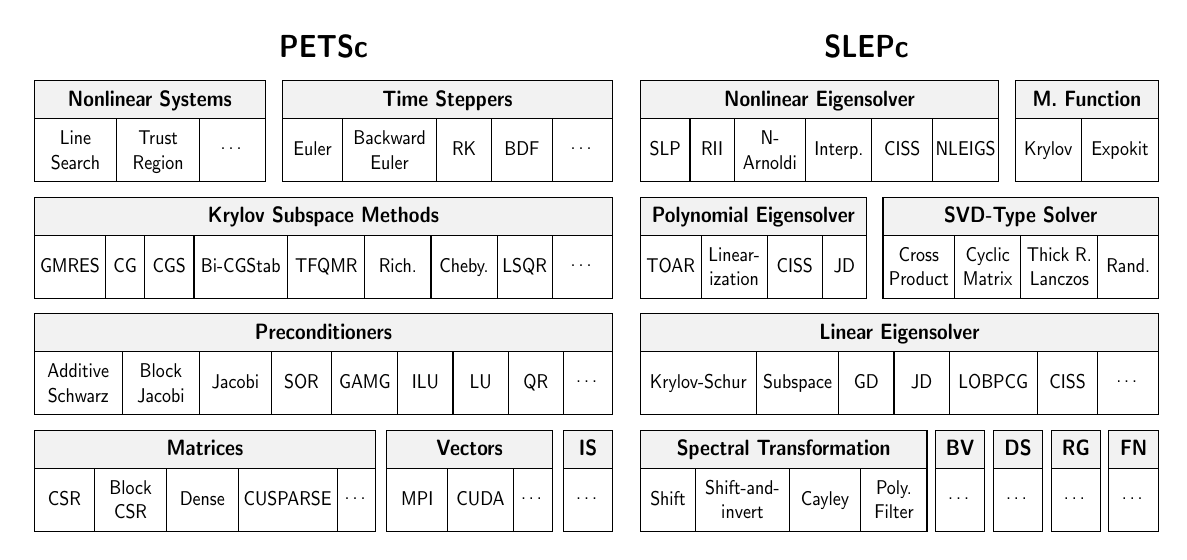
\begin{tikzpicture}[xscale=0.7,yscale=0.8]
  \tikzstyle{interface}=[fill=black!5,font=\sffamily\bfseries,text depth=.25ex]
  \tikzstyle{implem}=[font=\sffamily\small,text badly centered]
  \tikzstyle{every node}=[transform shape]
  \tikzstyle{onel}=[text depth=.25ex]
  \def\levsep{1.85} % separation of levels
  \def\hint{0.6} % height interface
  \def\himp{1} % height implementation
  \node[above,text centered,font=\sffamily\bfseries\Large] at (5.25,5*\levsep) {PETSc};
  \draw[interface] (0,\levsep+\himp) rectangle node {Matrices} +(6.2,\hint);
  \draw[implem] (0,\levsep) rectangle node[onel] {CSR} ++(1.1,1) ++(0,-1)
                rectangle node[text width=1.3cm] {Block CSR} ++(1.3,1) ++(0,-1)
                rectangle node[onel] {Dense} ++(1.3,1) ++(0,-1)
                rectangle node[onel] {CUSPARSE} ++(1.8,1) ++(0,-1)
                rectangle node[onel] {\dots} ++(.7,1);
  \draw[interface] (6.4,\levsep+\himp) rectangle node {Vectors} +(3,\hint);
  \draw[implem] (6.4,\levsep) rectangle node[onel] {MPI} ++(1.1,1) ++(0,-1)
                      rectangle node[onel] {CUDA} ++(1.2,1) ++(0,-1)
                      rectangle node[onel] {\dots} ++(.7,1);
  \draw[interface] (9.6,\levsep+\himp) rectangle node {IS} +(.9,\hint);
  \draw[implem] (9.6,\levsep) rectangle node[onel] {\dots} ++(.9,1);
  \draw[interface] (0,2*\levsep+\himp) rectangle node {Preconditioners} +(10.5,\hint);
  \draw[implem] (0,2*\levsep) rectangle node[text width=1.6cm] {Additive Schwarz} ++(1.6,1) ++(0,-1)
                rectangle node[text width=1.2cm] {Block Jacobi} ++(1.4,1) ++(0,-1)
                rectangle node[onel] {Jacobi} ++(1.3,1) ++(0,-1)
                rectangle node[onel] {SOR} ++(1.1,1) ++(0,-1)
                rectangle node[onel] {GAMG} ++(1.2,1) ++(0,-1)
                rectangle node[onel] {ILU} ++(1,1) ++(0,-1)
                rectangle node[onel] {LU} ++(1,1) ++(0,-1)
                rectangle node[onel] {QR} ++(1,1) ++(0,-1)
                rectangle node[onel] {\dots} ++(.9,1);
  \draw[interface] (0,3*\levsep+\himp) rectangle node {Krylov Subspace Methods} +(10.5,\hint);
  \draw[implem] (0,3*\levsep) rectangle node[onel] {GMRES} ++(1.3,1) ++(0,-1)
                rectangle node[onel] {CG} ++(0.7,1) ++(0,-1)
                rectangle node[onel] {CGS} ++(0.9,1) ++(0,-1)
                rectangle node[onel] {Bi-CGStab} ++(1.7,1) ++(0,-1)
                rectangle node[onel] {TFQMR} ++(1.4,1) ++(0,-1)
                rectangle node[onel] {Rich.} ++(1.2,1) ++(0,-1)
                rectangle node[onel] {Cheby.} ++(1.2,1) ++(0,-1)
                rectangle node[onel] {LSQR} ++(1,1) ++(0,-1)
                rectangle node[onel] {\dots} ++(1.1,1);
  \draw[interface] (0,4*\levsep+\himp) rectangle node {Nonlinear Systems} +(4.2,\hint);
  \draw[implem] (0,4*\levsep) rectangle node[text width=1.2cm] {Line Search} ++(1.5,1) ++(0,-1)
                rectangle node[text width=1.2cm,yshift=-1pt] {Trust Region} ++(1.5,1) ++(0,-1)
                rectangle node[onel] {\dots} ++(1.2,1);
  \draw[interface] (4.5,4*\levsep+\himp) rectangle node {Time Steppers} +(6,\hint);
  \draw[implem] (4.5,4*\levsep) rectangle node[onel] {Euler} ++(1.1,1) ++(0,-1)
                rectangle node[text width=1.5cm] {Backward Euler} ++(1.7,1) ++(0,-1)
                rectangle node[onel] {RK} ++(1.0,1) ++(0,-1)
                rectangle node[onel] {BDF} ++(1.1,1) ++(0,-1)
                rectangle node[onel] {\dots} ++(1.1,1);
  \node[above,text centered,font=\sffamily\bfseries\Large] at (15.1,5*\levsep) {SLEPc};
  \draw[interface] (11,4*\levsep+\himp) rectangle node {Nonlinear Eigensolver} +(6.5,\hint);
  \draw[implem] (11,4*\levsep) rectangle node[onel] {SLP} ++(.9,1) ++(0,-1)
                rectangle node[onel] {RII} ++(.8,1) ++(0,-1)
                rectangle node[text width=1.2cm] {N-Arnoldi} ++(1.3,1) ++(0,-1)
                rectangle node[onel] {Interp.} ++(1.2,1) ++(0,-1)
                rectangle node[onel] {CISS} ++(1.1,1) ++(0,-1)
                rectangle node[onel] {NLEIGS} ++(1.2,1);
  \draw[interface] (17.8,4*\levsep+\himp) rectangle node {M.~Function} +(2.6,\hint);
  \draw[implem] (17.8,4*\levsep) rectangle node[onel] {Krylov} ++(1.2,1) ++(0,-1)
                rectangle node[onel] {Expokit} ++(1.4,1);
  \draw[interface] (11,3*\levsep+\himp) rectangle node {Polynomial Eigensolver} +(4.1,\hint);
  \draw[implem] (11,3*\levsep) rectangle node[onel] {TOAR} ++(1.1,1) ++(0,-1)
                rectangle node[text width=1.2cm] {Linear\-ization} ++(1.2,1) ++(0,-1)
                rectangle node[onel] {CISS} ++(1,1) ++(0,-1)
                rectangle node[onel] {JD} ++(.8,1) ++(0,-1);
  \draw[interface] (15.4,3*\levsep+\himp) rectangle node {SVD-Type Solver} +(5,\hint);
  \draw[implem] (15.4,3*\levsep) rectangle node[text width=1.2cm] {Cross Product} ++(1.3,1) ++(0,-1)
                rectangle node[text width=1.2cm] {Cyclic Matrix} ++(1.2,1) ++(0,-1)
                rectangle node[text width=1.4cm] {Thick R. Lanczos} ++(1.4,1) ++(0,-1)
                rectangle node[onel] {Rand.} ++(1.1,1);
  \draw[interface] (11,2*\levsep+\himp) rectangle node {Linear Eigensolver} +(9.4,\hint);
  \draw[implem] (11,2*\levsep) rectangle node[onel] {Krylov-Schur} ++(2.1,1) ++(0,-1)
                rectangle node[onel] {Subspace} ++(1.5,1) ++(0,-1)
                rectangle node[onel] {GD} ++(1.0,1) ++(0,-1)
                rectangle node[onel] {JD} ++(1.0,1) ++(0,-1)
                rectangle node[onel] {LOBPCG} ++(1.6,1) ++(0,-1)
                rectangle node[onel] {CISS} ++(1.1,1) ++(0,-1)
                rectangle node[onel] {\dots} ++(1.1,1);
  \draw[interface] (11,\levsep+\himp) rectangle node {Spectral Transformation} +(5.2,\hint);
  \draw[implem] (11,\levsep) rectangle node[onel] {Shift} ++(1,1) ++(0,-1)
                rectangle node[text width=1.6cm] {Shift-and-invert} ++(1.7,1) ++(0,-1)
                rectangle node[onel] {Cayley} ++(1.3,1) ++(0,-1)
                rectangle node[text width=1.2cm] {Poly. Filter} ++(1.2,1);
  \draw[interface] (16.35,\levsep+\himp) rectangle node {BV} +(.9,\hint) ++(1.05,0)
                   rectangle node {DS} +(.9,\hint) ++(1.05,0)
                   rectangle node {RG} +(.9,\hint) ++(1.05,0)
                   rectangle node {FN} +(.9,\hint);
  \draw[implem] (16.35,\levsep) rectangle node[onel] {\dots} ++(.9,1);
  \draw[implem] (17.4,\levsep) rectangle node[onel] {\dots} ++(.9,1);
  \draw[implem] (18.45,\levsep) rectangle node[onel] {\dots} ++(.9,1);
  \draw[implem] (19.5,\levsep) rectangle node[onel] {\dots} ++(.9,1);
\end{tikzpicture}
\caption{\label{fig:slepc}Numerical components of \petsc and \slepc.}
\end{figure}

Each of these components consists of an abstract interface (simply a set of calling sequences) and one or more implementations using particular data structures. Both \petsc and \slepc are written in C, which lacks direct support for object-oriented programming. However, it is still possible to take advantage of the three basic principles of object-oriented programming to manage the complexity of such large packages. \petsc uses data \emph{encapsulation} in both vector and matrix data objects. Application code accesses data through function calls. Also, all the operations are supported through \emph{polymorphism}. The user calls a generic interface routine, which then selects the underlying routine that handles the particular data structure. Finally, \petsc also uses \emph{inheritance} in its design. All the objects are derived from an abstract base object. From this fundamental object, an abstract base object is defined for each \petsc\ object (\texttt{Mat}, \texttt{Vec} and so on), which in turn has a variety of instantiations that, for example, implement different matrix storage formats.

\petsc/\slepc provide clean and effective codes for the various phases of solving PDEs, with a uniform approach for each class of problems.  This design enables easy comparison and use of different algorithms (for example, to experiment with different Krylov subspace methods, preconditioners, or eigensolvers). Hence, \petsc, together with \slepc, provides a rich environment for modeling scientific applications as well as for rapid algorithm design and prototyping.

Options can be specified by means of calls to subroutines in the source code and also as command-line arguments. Runtime options allow the user to test different tolerances, for example, without having to recompile the program. Also, since \petsc provides a uniform interface to all of its linear solvers ---the Conjugate Gradient, GMRES, etc.--- and a large family of preconditioners ---block Jacobi, overlapping additive Schwarz, etc.---, one can compare several combinations of method and preconditioner by simply specifying them at execution time. \slepc shares this good property.

The components enable easy customization and extension of both algorithms and implementations. This approach promotes code reuse and flexibility, and separates the issues of parallelism from the choice of algorithms.  The \petsc infrastructure creates a foundation for building large-scale applications.

%---------------------------------------------------
\section{Installation}
\label{sec:inst}

This section describes \slepc's installation procedure.
Previously to the installation of \slepc, the system must have an appropriate version of \petsc\ installed. Compatible versions of \petsc and \slepc are those with coincident major and minor version number, the third number (patch level) being irrelevant for this. For instance, \slepc 3.23.x may be built with \petsc 3.23.x. Also note that, if using git repositories, both \petsc and \slepc must be either release versions or development versions, so make sure you select the appropriate branch in both repositories (\texttt{git checkout release} or \texttt{git checkout main}).

The installation process for \slepc is very similar to \petsc, with two stages: configuration and compilation. \slepc's configuration is much simpler because most of the configuration information is taken from \petsc, including compiler options and scalar type (real or complex). See \S\ref{sec:opt-inst} for a discussion of options that are most relevant for \slepc. Several configurations can coexist in the same directory tree, so that for instance one can have \slepc libraries compiled with real scalars as well as with complex scalars. This is explained in \S\ref{sec:mult-inst}. Also, system-based installation is also possible with the \Verb!--prefix! option, as discussed in \S\ref{sec:prefix-inst}.

\subsection{Standard Installation}
\label{sec:std-inst}

The basic steps for the installation are described next. Note that prior to these steps, optional packages must have been installed. If any of these packages is installed afterwards, reconfiguration and recompilation is necessary. Refer to \S\ref{sec:opt-inst} and \S\ref{sec:wrap} for details about installation of some of these packages.

\begin{enumerate}
\item Unbundle the distribution file with
        \begin{Verbatim}[fontsize=\small]
        $ tar xzf slepc-3.23.0.tar.gz
        \end{Verbatim}
        or an equivalent command. This will create a directory and unpack the software there.
\item Set the environment variable \ident{SLEPC\_DIR} to the full path of the \slepc home directory. For example, under the \texttt{bash} shell:
        \begin{Verbatim}[fontsize=\small]
        $ export SLEPC_DIR=/home/username/slepc-3.23.0
        \end{Verbatim}
In addition, the variables \ident{PETSC\_DIR} and \ident{PETSC\_ARCH} must also be set appropriately, e.g.
        \begin{Verbatim}[fontsize=\small]
        $ export PETSC_DIR=/home/username/petsc-3.23.0
        $ export PETSC_ARCH=arch-darwin-c-debug
        \end{Verbatim}
        The rationale for \ident{PETSC\_ARCH} is explained in \S\ref{sec:mult-inst} (see \S\ref{sec:prefix-inst} for a case in which \ident{PETSC\_ARCH} is not required).
\item\label{step-config} Change to the \slepc directory and run the configuration script:
        \begin{Verbatim}[fontsize=\small]
        $ cd $SLEPC_DIR
        $ ./configure
        \end{Verbatim}
\item If the configuration was successful, build the libraries:
        \begin{Verbatim}[fontsize=\small]
        $ make
        \end{Verbatim}
\item After the compilation, try running some test examples with
        \begin{Verbatim}[fontsize=\small]
        $ make check
        \end{Verbatim}
        Examine the output for any obvious errors or problems.
\end{enumerate}

\subsection{Configuration Options}
\label{sec:opt-inst}

Several options are available in \slepc's configuration script. To see all available options, type \Verb!./configure --help!.

In \slepc, configure options have the following purposes:
\begin{itemize}
%\item Build \slepc with Python interfaces, as explained in \S\ref{sec:py-inst}.
\item Specify a directory for prefix-based installation, as explained in \S\ref{sec:prefix-inst}.
\item Enable external eigensolver packages. For example, to use \arpack, specify the following options (with the appropriate paths):
        \begin{Verbatim}[fontsize=\small]
        $ ./configure --with-arpack-dir=/usr/software/ARPACK
        \end{Verbatim}
Some of the external packages also support the \Verb!--download-xxxx! option. Section \ref{sec:wrap} provides more details related to use of external libraries.
\end{itemize}

Additionally, \petsc's configuration script provides a very long list of options that are relevant to \slepc. Here is a list of options that may be useful. Note that these are options of \petsc that apply to both \petsc and \slepc, in such a way that it is not possible to, e.g., build \petsc without debugging and \slepc with debugging.
\begin{itemize}
\item Add \Verb!--with-scalar-type=complex! to build complex scalar versions of all libraries. See below a note related to complex scalars.
\item Build single precision versions with \Verb!--with-precision=single!. In most applications, this can achieve a significant reduction of memory requirements, and a moderate reduction of computing time. Also, quadruple precision (128-bit floating-point representation) is also available using \Verb!--with-precision=__float128! on systems with GNU compilers (\texttt{gcc-4.6} or later).
\item Enable use from Fortran. By default, \petsc's configure looks for an appropriate Fortran compiler. If not required, this can be disabled: \Verb!--with-fc=0!. If required but not correctly detected, the compiler to be used can be specified with a configure option. It is also possible to configure with a Fortran compiler but do not build Fortran interfaces of \petsc and \slepc, with \Verb!--with-fortran-bindings=0!.
\item If not detected, use \Verb!--with-blas-lapack-lib! to specify the location of \blas and \lapack. If \slepc's configure complains about some missing \lapack subroutines, reconfigure \petsc with option \Verb!--download-f2cblaslapack!.
\item Enable external libraries that provide direct linear solvers or preconditioners, such as MUMPS, hypre, or SuperLU; for example, \Verb!--download-mumps!. These are especially relevant for \slepc in the case that a spectral transformation is used, see chapter \ref{cap:st}.
\item Add \Verb!--with-64-bit-indices=1! to use 8 byte integers (\texttt{long long}) for indexing in vectors and matrices. This is only needed when working with over roughly 2 billion unknowns.
\item Build static libraries, \Verb!--with-shared-libraries=0!. This is generally not recommended, since shared libraries produce smaller executables and the run time overhead is small.
\item Error-checking code can be disabled with \Verb!--with-debugging=0!, but this is only recommended in production runs of well-tested applications.
\item Enable GPU computing setting \Verb!--with-cuda=1! or \Verb!--with-hip=1!; see \S\ref{sec:gpu} for details.
\item The option \Verb!--with-mpi=0! allows building \petsc and \slepc without MPI support (only sequential).
\end{itemize}

\medskip
\textbf{Note about complex scalar versions}: \petsc supports the use of complex scalars by defining the data type \ident{PetscScalar} either as a real or complex number. This implies that two different versions of the \petsc libraries can be built separately, one for real numbers and one for complex numbers, but they cannot be used at the same time. \slepc inherits this property. In \slepc it is not possible to completely separate real numbers and complex numbers because the solution of non-symmetric real-valued eigenvalue problems may be complex. \slepc has been designed trying to provide a uniform interface to manage all the possible cases. However, there are slight differences between the interface in each of the two versions. In this manual, differences are clearly identified.

\subsection{Installing Multiple Configurations in a Single Directory Tree}
\label{sec:mult-inst}

Often, it is necessary to build two (or more) versions of the libraries that differ in a few configuration options. For instance, versions for real and complex scalars, or versions for double and single precision, or versions with debugging and optimized. In a standard installation, this is handled by building all versions in the same directory tree, as explained below, so that source code is not replicated unnecessarily. In contrast, in prefix-based installation where source code is not present, the issue of multiple configurations is handled differently, as explained in \S\ref{sec:prefix-inst}.

In a standard installation, the different configurations are identified by a unique name that is assigned to the environment variable \ident{PETSC\_ARCH}. Let us illustrate how to set up \petsc with two configurations. First, set a value of \ident{PETSC\_ARCH} and proceed with the installation of the first one:
        \begin{Verbatim}[fontsize=\small]
        $ cd $PETSC_DIR
        $ export PETSC_ARCH=arch-linux-gnu-c-debug-real
        $ ./configure --with-scalar-type=real
        $ make all
        \end{Verbatim}
Note that if \ident{PETSC\_ARCH} is not given a value, \petsc suggests one for us. After this, a subdirectory named \texttt{\$PETSC\_ARCH} is created within \texttt{\$PETSC\_DIR}, that stores all information associated with that configuration, including the built libraries, configuration files, automatically generated source files, and log files. For the second configuration, proceed similarly:
        \begin{Verbatim}[fontsize=\small]
        $ cd $PETSC_DIR
        $ export PETSC_ARCH=arch-linux-gnu-c-debug-complex
        $ ./configure --with-scalar-type=complex
        $ make all
        \end{Verbatim}
The value of \ident{PETSC\_ARCH} in this case must be different than the previous one. It is better to set the value of \ident{PETSC\_ARCH} explicitly, because the name suggested by \texttt{configure} may coincide with an existing value, thus overwriting a previous configuration. After successful installation of the second configuration, two \texttt{\$PETSC\_ARCH} directories exist within \texttt{\$PETSC\_DIR}, and the user can easily choose to build his/her application with either configuration by simply changing the value of \ident{PETSC\_ARCH}.

The configuration of two versions of \slepc in the same directory tree is very similar. The only important restriction is that the value of \ident{PETSC\_ARCH} used in \slepc must exactly match an existing \petsc configuration, that is, a directory \texttt{\$PETSC\_DIR/\$PETSC\_ARCH} must exist.

\subsection{Prefix-based Installation}
\label{sec:prefix-inst}

Both \petsc and \slepc allow for prefix-based installation. This consists in specifying a directory to which the files generated during the building process are to be copied.

In \petsc, if an installation directory has been specified during configuration (with option \Verb!--prefix! in step \ref{step-config} of \S\ref{sec:std-inst}), then after building the libraries the relevant files are copied to that directory by typing
        \begin{Verbatim}[fontsize=\small]
        $ make install
        \end{Verbatim}
This is useful for building as a regular user and then copying the libraries and include files to the system directories as root.

To be more precise, suppose that the configuration was done with \texttt{-{}-prefix=/opt/petsc-3.23.0-linux-gnu-c-debug}. Then, \texttt{make install} will create directory \texttt{/opt/petsc-3.23.0-linux-gnu-c-debug} if it does not exist, and several subdirectories containing the libraries, the configuration files, and the header files. Note that the source code files are not copied, nor the documentation, so the size of the installed directory will be much smaller than the original one. For that reason, it is no longer necessary to allow for several configurations to share a directory tree. In other words, in a prefix-based installation, variable \ident{PETSC\_ARCH} loses significance and must be unset. To maintain several configurations, one should specify different prefix directories, typically with a name that informs about the configuration options used.

In order to prepare a prefix-based installation of \slepc that uses a prefix-based installation of \petsc, start by setting the appropriate value of \ident{PETSC\_DIR}. Then, run \slepc's configure with a prefix directory.
        \begin{Verbatim}[fontsize=\small,numbers=none]
        $ export PETSC_DIR=/opt/petsc-3.23.0-linux-gnu-c-debug
        $ unset PETSC_ARCH
        $ cd $SLEPC_DIR
        $ ./configure --prefix=/opt/slepc-3.23.0-linux-gnu-c-debug
        $ make
        $ make install
        $ export SLEPC_DIR=/opt/slepc-3.23.0-linux-gnu-c-debug
        \end{Verbatim}
Note that the variable \ident{PETSC\_ARCH} has been unset before \slepc's configure. \slepc will use a temporary arch name during the build (this temporary arch is named \texttt{installed-arch-xxx}, where the \texttt{arch-xxx} string represents the configuration of the installed \petsc version). Although it is not a common case, it is also possible to configure \slepc without prefix, in which case the \ident{PETSC\_ARCH} variable must still be empty and the arch directory \texttt{installed-xxx} is picked automatically (it is hardwired in file \texttt{\$SLEPC\_DIR/lib/slepc/conf/slepcvariables}). The combination \petsc without prefix and \slepc with prefix is also allowed, in which case \ident{PETSC\_ARCH} should not be unset.

%\subsection{Building Python Interfaces}
%\label{sec:py-inst}

%---------------------------------------------------
\section{Running SLEPc Programs}

Before using \slepc, the user must first set the environment variable
\ident{SLEPC\_DIR}, indicating the full path of the directory containing \slepc. For example, under the \texttt{bash} shell, a command of the form
        \begin{Verbatim}[fontsize=\small]
        $ export SLEPC_DIR=/software/slepc-3.23.0
        \end{Verbatim}
can be placed in the user's \Verb!.bashrc! file.
The \ident{SLEPC\_DIR} directory can be either a standard installation \slepc directory, or a prefix-based installation directory, see \S\ref{sec:prefix-inst}.
In addition, the user must set the environment variables required by \petsc, that is, \ident{PETSC\_DIR}, to indicate the full path of the \petsc directory, and \ident{PETSC\_ARCH} to specify a particular architecture and set of options. Note that \ident{PETSC\_ARCH} should not be set in the case of prefix-based installations.

All \petsc programs use the MPI (Message Passing Interface) standard
for message-passing communication \citep{MPI-Forum:1994:MMI}.  Thus, to execute
\slepc programs, users must know the procedure for launching MPI jobs
on their selected computer system(s).  Usually, the \texttt{mpiexec} command can be used to initiate a program as in the following example that uses eight processes:
        \begin{Verbatim}[fontsize=\small]
        $ mpiexec -n 8 slepc_program [command-line options]
        \end{Verbatim}
Note that MPI may be deactivated during configuration of \petsc, if one wants to run only serial programs in a laptop, for example.

All \petsc-compliant programs support the use of the \Verb!-h!
or \Verb!-help! option as well as the \Verb!-v! or \Verb!-version! option. In the case of \slepc programs, specific information for \slepc is also displayed.

%---------------------------------------------------
\section{Writing SLEPc Programs}

Most \slepc programs begin with a call to \rutina{SlepcInitialize}
        \begin{Verbatim}[fontsize=\small]
        SlepcInitialize(int *argc,char ***argv,char *file,char *help);
        \end{Verbatim}
which initializes \slepc, \petsc and MPI. This subroutine is very similar to \rutina{PetscInitialize}, and the arguments have the same meaning. In fact, internally \rutina{SlepcInitialize} calls \rutina{PetscInitialize}.

After this initialization, \slepc programs can use communicators defined by \petsc. In most cases users can employ the communicator \ident{PETSC\_COMM\_WORLD} to indicate all processes in a given run and \ident{PETSC\_COMM\_SELF} to indicate a single process. MPI provides routines for generating new communicators consisting of subsets of processes, though most users rarely need to use these features. \slepc users need not program much message passing directly with MPI, but they must be familiar with the basic concepts of message passing and distributed memory computing.

All \slepc programs should call \rutina{SlepcFinalize} as their final (or nearly final) statement
        \begin{Verbatim}[fontsize=\small]
        SlepcFinalize();
        \end{Verbatim}
This routine handles operations to be executed at the conclusion of the program, and calls \rutina{PetscFinalize} if \rutina{SlepcInitialize} began \petsc.

\medskip
\textbf{Note to Fortran Programmers}: In this manual all the examples and calling sequences are given for the C/C++ programming languages. However, Fortran programmers can use most of the functionality of \slepc and \petsc from Fortran, with only minor differences in the user interface. For instance, the two functions mentioned above have their corresponding Fortran equivalent:
        \begin{Verbatim}[fontsize=\small]
        call SlepcInitialize(file,ierr)
        call SlepcFinalize(ierr)
        \end{Verbatim}
Section \ref{sec:fortran} provides a summary of the differences between using \slepc from Fortran and C/C++, as well as a complete Fortran example.

%---------------------------------------------------
\subsection{Simple SLEPc Example}
\label{sec:simpleex}

A simple example is listed next that solves an eigenvalue problem associated with the one-dimensional Laplacian operator discretized with finite differences. This example can be found in \Verb!${SLEPC_DIR}/src/eps/tutorials/ex1.c!. Following the code we highlight a few of the most important parts of this example.

\MyVerbatimInput{ex1.c}

\paragraph{Include Files.}

The C/C++ include files for \slepc should be used via statements such as
        \begin{Verbatim}[fontsize=\small]
        #include <slepceps.h>
        \end{Verbatim}
where \Verb!slepceps.h! is the include file for the \ident{EPS} component. Each \slepc program must specify an include file that corresponds to the highest level \slepc objects needed within the program; all of the required lower level include files are automatically included within the higher level files. For example, \Verb!slepceps.h! includes \Verb!slepcst.h! (spectral transformations), and \Verb!slepcsys.h! (base \slepc file). Some \petsc header files are included as well, such as \Verb!petscksp.h!. The \slepc include files are located in the directory \Verb!${SLEPC_DIR}/include!.

\paragraph{The Options Database.}

All the \petsc functionality related to the options database is available in \slepc. This allows the user to input control data at run time very easily. In this example, the call \Verb!PetscOptionsGetInt(NULL,NULL,"-n",&n,NULL)! checks whether the user has provided a command line option to set the value of \Verb!n!, the problem dimension.  If so, the variable \Verb!n! is set accordingly; otherwise, \Verb!n! remains unchanged.

\paragraph{Vectors and Matrices.}

Usage of matrices and vectors in \slepc is exactly the same as in \petsc. The user can create a new parallel or sequential matrix, \texttt{A}, which has \texttt{M} global rows and \texttt{N} global columns, with
        \begin{Verbatim}[fontsize=\small]
        MatCreate(MPI_Comm comm,Mat *A);
        MatSetSizes(Mat A,PetscInt m,PetscInt n,PetscInt M,PetscInt N);
        MatSetFromOptions(Mat A);
        \end{Verbatim}
where the matrix format can be specified at runtime. The example creates a matrix, sets the nonzero values with \rutina{MatSetValues} and then assembles it.

\paragraph{Eigensolvers.}

Usage of eigensolvers is very similar to other kinds of solvers provided by \petsc. After creating the matrix (or matrices) that define the problem, $Ax = kx$ (or $Ax=kBx$), the user can then use \ident{EPS} to solve the system with the following sequence of commands:
\findex{EPSCreate} \findex{EPSSetOperators} \findex{EPSSetProblemType}
\findex{EPSSetFromOptions} \findex{EPSSolve} \findex{EPSDestroy}
\findex{EPSGetConverged} \findex{EPSGetEigenpair}
        \begin{Verbatim}[fontsize=\small,numbers=none]
        EPSCreate(MPI_Comm comm,EPS *eps);
        EPSSetOperators(EPS eps,Mat A,Mat B);
        EPSSetProblemType(EPS eps,EPSProblemType type);
        EPSSetFromOptions(EPS eps);
        EPSSolve(EPS eps);
        EPSGetConverged(EPS eps,PetscInt *nconv);
        EPSGetEigenpair(EPS eps,PetscInt i,PetscScalar *kr,PetscScalar *ki,Vec xr,Vec xi);
        EPSDestroy(EPS *eps);
        \end{Verbatim}
The user first creates the \ident{EPS} context and sets the operators associated with the eigensystem as well as the problem type. The user then sets various options for customized solution, solves the problem, retrieves the solution, and finally destroys the \ident{EPS} context. Chapter~\ref{cap:eps} describes in detail the \ident{EPS} package, including
the options database that enables the user to customize the solution process at runtime by selecting the solution algorithm and also specifying the convergence tolerance, the number of eigenvalues, the dimension of the subspace, etc.

\paragraph{Spectral Transformation.}

In the example program shown above there is no explicit reference to spectral transformations. However, an \ident{ST} object is handled internally so that the user is able to request different transformations such as shift-and-invert. Chapter~\ref{cap:st} describes the \ident{ST} package in detail.

\paragraph{Error Checking.}

All \slepc routines return an integer indicating whether an error has occurred during the call. The error code is set to be nonzero if an error has been detected; otherwise, it is zero. The \petsc macro \Verb!PetscCall(...)! checks the return value and calls the \petsc error handler upon error detection. \Verb!PetscCall(...)! should be used in all subroutine calls to enable a complete error traceback. See the \petsc documentation for full details.

\subsection{Writing Application Codes with SLEPc}

Several example programs demonstrate the software usage and can serve as templates for developing custom applications. They are scattered throughout the \slepc directory tree, in particular in the \Verb!tutorials! directories under each class subdirectory.

To write a new application program using \slepc, we suggest the following procedure:
\begin{enumerate}
\item Install and test \slepc according to the instructions given in the documentation.
\item Copy the \slepc example that corresponds to the class of problem of interest (e.g., singular value decomposition).
\item Create a makefile as explained below, compile and run the example program.
\item Use the example program as a starting point for developing a custom code.
\end{enumerate}

Application program makefiles can be set up very easily just by including one file from the \slepc makefile system. All the necessary \petsc{} definitions are loaded automatically. The following sample makefile illustrates how to build C and Fortran programs:

\begin{Verbatim}[fontsize=\small]
default: ex1

include ${SLEPC_DIR}/lib/slepc/conf/slepc_common

ex1: ex1.o
        -${CLINKER} -o ex1 ex1.o ${SLEPC_EPS_LIB}
        ${RM} ex1.o

ex1f: ex1f.o
        -${FLINKER} -o ex1f ex1f.o ${SLEPC_EPS_LIB}
        ${RM} ex1f.o
\end{Verbatim}


%-------------------------------------------------------
% SLEPc Users Manual
%-------------------------------------------------------
\chapter{\label{cap:eps}EPS: Eigenvalue Problem Solver}
%-------------------------------------------------------

\noindent The Eigenvalue Problem Solver (\ident{EPS}) is the main object provided by \slepc. It is used to specify a linear eigenvalue problem, either in standard or generalized form, and provides uniform and efficient access to all of the linear eigensolvers included in the package. Conceptually, the level of abstraction occupied by \ident{EPS} is similar to other solvers in \petsc\ such as \ident{KSP} for solving linear systems of equations.

\section{\label{sec:eig}Eigenvalue Problems}

In this section, we briefly present some basic concepts about eigenvalue problems as well as general techniques used to solve them. The description is not intended to be exhaustive. The objective is simply to define terms that will be referred to throughout the rest of the manual. Readers who are familiar with the terminology and the solution approach can skip this section. For a more comprehensive description, we refer the reader to monographs such as \citep{Stewart:2001:MAV}, \citep{Bai:2000:TSA}, \citep{Saad:1992:NML} or \citep{Parlett:1980:SEP}. A historical perspective of the topic can be found in \citep{Golub:2000:EC2}. See also the \slepc \hyperlink{str}{technical reports}.

In the standard formulation, the linear eigenvalue problem consists in the determination of $\lambda\in\mathbb{C}$ for which the equation
\begin{equation}
Ax=\lambda x\label{eq:eigstd}
\end{equation}
has nontrivial solution, where $A\in\mathbb{C}^{n\times n}$ and $x\in\mathbb{C}^n$. The scalar $\lambda$ and the vector $x$ are called eigenvalue and (right) eigenvector, respectively. Note that they can be complex even when the matrix is real. If $\lambda$ is an eigenvalue of $A$ then $\bar{\lambda}$ is an eigenvalue of its conjugate transpose, $A^*$, or equivalently
\begin{equation}
y^*\!A=\lambda\, y^*,\label{eq:eigstdleft}
\end{equation}
where $y$ is called the left eigenvector.

In many applications, the problem is formulated as
\begin{equation}
Ax=\lambda Bx,\label{eq:eiggen}
\end{equation}
where $B\in\mathbb{C}^{n\times n}$, which is known as the generalized eigenvalue problem. Usually, this problem is solved by reformulating it in standard form, for example $B^{-1}Ax=\lambda x$ if $B$ is non-singular.

\slepc focuses on the solution of problems in which the matrices are large and sparse. Hence, only methods that preserve sparsity are considered.
These methods obtain the solution from the information generated by the application of the operator to various vectors (the operator is a simple function of matrices $A$ and $B$), that is, matrices are only used in matrix-vector products. This not only maintains sparsity but allows the solution of problems in which matrices are not available explicitly.

In practical analyses, from the $n$ possible solutions, typically only a few eigenpairs $(\lambda,x)$ are considered relevant, either in the extremities of the spectrum, in an interval, or in a region of the complex plane.
Depending on the application, either eigenvalues or eigenvectors (or both) are required. In some cases, left eigenvectors are also of interest.

\paragraph{Projection Methods.}

Most eigensolvers provided by \slepc perform a Rayleigh-Ritz projection for extracting the spectral approximations, that is, they project the problem onto a low-dimensional subspace that is built appropriately. Suppose that an orthogonal basis of this subspace is given by $V_j=[v_1,v_2,\ldots,v_j]$. If the solutions of the projected (reduced) problem $B_js=\theta s$ (i.e., $V_j^TAV_j=B_j$) are assumed to be $(\theta_i,s_i)$, $i=1,2,\ldots,j$, then the approximate eigenpairs $(\tilde{\lambda}_i,\tilde{x}_i)$ of the original problem (Ritz value and Ritz vector) are obtained as
\begin{eqnarray}
\tilde{\lambda}_i=\theta_i,\\
\tilde{x}_i=V_js_i.
\end{eqnarray}
Starting from this general idea, eigensolvers differ from each other in which subspace is used, how it is built and other technicalities aimed at improving convergence, reducing storage requirements, etc.

The subspace
\begin{equation}
\mathcal{K}_m(A,v)\equiv\mathrm{span}\left\{v,Av,A^2v,\ldots,A^{m-1}v\right\},\label{eq:krylov}
\end{equation}
is called the $m$-th Krylov subspace corresponding to $A$ and $v$. Methods that use subspaces of this kind to carry out the projection are called Krylov methods. One example of such methods is the Arnoldi algorithm: starting with $v_1$, $\|v_1\|_2=1$, the Arnoldi basis generation process can be expressed by the recurrence
\begin{equation}
v_{j+1}h_{j+1,j}=w_j=Av_j-\sum_{i=1}^jh_{i,j}v_i,
\end{equation}
where $h_{i,j}$ are the scalar coefficients obtained in the Gram-Schmidt orthogonalization of $Av_j$ with respect to $v_i$, $i=1,2,\ldots,j$, and $h_{j+1,j}=\|w_j\|_2$. Then, the columns of $V_j$ span the Krylov subspace $\mathcal{K}_j(A,v_1)$ and $Ax=\lambda x$ is projected into $H_js=\theta s$, where $H_j$ is an upper Hessenberg matrix with elements $h_{i,j}$, which are 0 for $i\geq j+2$. The related Lanczos algorithms obtain a projected matrix that is tridiagonal.

A generalization to the above methods are the block Krylov strategies, in which the starting vector $v_1$ is replaced by a full rank $n\times p$ matrix $V_1$, which allows for better convergence properties when there are multiple eigenvalues and can provide better data management on some computer architectures. Block tridiagonal and block Hessenberg matrices are then obtained as projections.

It is generally assumed (and observed) that the Lanczos and Arnoldi algorithms find solutions at the extremities of the spectrum. Their convergence pattern, however, is strongly related to the eigenvalue distribution. Slow convergence may be experienced in the presence of tightly clustered eigenvalues. The maximum allowable $j$ may be reached without having achieved convergence for all desired solutions. Then, restarting is usually a useful technique and different strategies exist for that purpose. However, convergence can still be very slow and acceleration strategies must be applied. Usually, these techniques consist in computing eigenpairs of a transformed operator and then recovering the solution of the original problem. The aim of these transformations is twofold. On one hand, they make it possible to obtain eigenvalues other than those lying in the periphery of the spectrum. On the other hand, the separation of the eigenvalues of interest is improved in the transformed spectrum thus leading to faster convergence. The most commonly used spectral transformation is called shift-and-invert, which works with operator $(A-\sigma I)^{-1}$. It allows the computation of eigenvalues closest to $\sigma$ with very good separation properties. When using this approach, a linear system of equations, $(A-\sigma I)y=x$, must be solved in each iteration of the eigenvalue process.

\paragraph{Preconditioned Eigensolvers.}
In many applications, Krylov eigensolvers perform very well because Krylov subspaces are optimal in a certain theoretical sense. However, these methods may not be appropriate in some situations such as the computation of interior eigenvalues. The spectral transformation mentioned above may not be a viable solution or it may be too costly. For these reasons, other types of eigensolvers such as Davidson and Jacobi-Davidson rely on a different way of expanding the subspace. Instead of satisfying the Krylov relation, these methods compute the new basis vector by the so-called correction equation. The resulting subspace may be richer in the direction of the desired eigenvectors. These solvers may be competitive especially for computing interior eigenvalues. From a practical point of view, the correction equation may be seen as a cheap replacement for the shift-and-invert system of equations, $(A-\sigma I)y=x$. By cheap we mean that it may be solved inaccurately without compromising robustness, via a preconditioned iterative linear solver. For this reason, these are known as \emph{preconditioned} eigensolvers.

\paragraph{Related Problems.}

In many applications such as the analysis of damped vibrating systems the problem to be solved is a \emph{polynomial eigenvalue problem} (PEP), or more generally a \emph{nonlinear eigenvalue problem} (NEP). For these, the reader is referred to chapters \ref{cap:pep} and \ref{cap:nep}. Another linear algebra problem that is very closely related to the eigenvalue problem is the {\em singular value decomposition\/} (SVD), see chapter \ref{cap:svd}.

%---------------------------------------------------
\section{Basic Usage}

The \ident{EPS} module in \slepc is used in a similar way as \petsc modules such as \ident{KSP}. All the information related to an eigenvalue problem is handled via a context variable. The usual object management functions are available (\ident{EPSCreate}, \ident{EPSDestroy}, \ident{EPSView}, \ident{EPSSetFromOptions}). In addition, the \ident{EPS} object provides functions for setting several parameters such as the number of eigenvalues to compute, the dimension of the subspace, the portion of the spectrum of interest, the requested tolerance or the maximum number of iterations allowed.

The solution of the problem is obtained in several steps. First of all, the matrices associated with the eigenproblem are specified via \ident{EPSSetOperators} and \ident{EPSSetProblemType} is used to specify the type of problem. Then, a call to \ident{EPSSolve} is done that invokes the subroutine for the selected eigensolver. \ident{EPSGetConverged} can be used afterwards to determine how many of the requested eigenpairs have converged to working accuracy. \ident{EPSGetEigenpair} is finally used to retrieve the eigenvalues and eigenvectors.

In order to illustrate the basic functionality of the \ident{EPS} package, a simple example is shown in Figure \ref{fig:ex-eps}. The example code implements the solution of a simple standard eigenvalue problem. Code for setting up the matrix $A$ is not shown and error-checking code is omitted.

\begin{figure}
\begin{Verbatim}[fontsize=\small,numbers=left,numbersep=6pt,xleftmargin=15mm]
EPS         eps;       /*  eigensolver context  */
Mat         A;         /*  matrix of Ax=kx      */
Vec         xr, xi;    /*  eigenvector, x       */
PetscScalar kr, ki;    /*  eigenvalue, k        */
PetscInt    j, nconv;
PetscReal   error;

EPSCreate( PETSC_COMM_WORLD, &eps );
EPSSetOperators( eps, A, NULL );
EPSSetProblemType( eps, EPS_NHEP );
EPSSetFromOptions( eps );
EPSSolve( eps );
EPSGetConverged( eps, &nconv );
for (j=0; j<nconv; j++) {
  EPSGetEigenpair( eps, j, &kr, &ki, xr, xi );
  EPSComputeError( eps, j, EPS_ERROR_RELATIVE, &error );
}
EPSDestroy( &eps );
\end{Verbatim}
\caption{\label{fig:ex-eps}Example code for basic solution with \ident{EPS}.}
\end{figure}

All the operations of the program are done over a single \ident{EPS} object. This solver context is created in line 8 with the command
        \findex{EPSCreate}
        \begin{Verbatim}[fontsize=\small]
        EPSCreate(MPI_Comm comm,EPS *eps);
        \end{Verbatim}
Here \texttt{comm} is the MPI communicator, and \texttt{eps} is the newly formed solver context. The communicator indicates which processes are involved in the \ident{EPS} object. Most of the \ident{EPS} operations are collective, meaning that all the processes collaborate to perform the operation in parallel.

Before actually solving an eigenvalue problem with \ident{EPS}, the user must specify the matrices associated with the problem, as in line 9, with the following routine
        \findex{EPSSetOperators}
        \begin{Verbatim}[fontsize=\small]
        EPSSetOperators(EPS eps,Mat A,Mat B);
        \end{Verbatim}
The example specifies a standard eigenproblem. In the case of a generalized problem, it would be necessary also to provide matrix $B$ as the third argument to the call. The matrices specified in this call can be in any \petsc format. In particular, \ident{EPS} allows the user to solve matrix-free problems by specifying matrices created via \ident{MatCreateShell}. A more detailed discussion of this issue is given in \S\ref{sec:supported}.

After setting the problem matrices, the problem type is set with \ident{EPSSetProblemType}. This is not strictly necessary since if this step is skipped then the problem type is assumed to be non-symmetric. More details are given in \S\ref{sec:defprob}.
At this point, the value of the different options could optionally be set by means of a function call such as \ident{EPSSetTolerances} (explained later in this chapter). After this, a call to \ident{EPSSetFromOptions} should be made as in line 11,
        \findex{EPSSetFromOptions}
        \begin{Verbatim}[fontsize=\small]
        EPSSetFromOptions(EPS eps);
        \end{Verbatim}
The effect of this call is that options specified at runtime in the command line are passed to the \ident{EPS} object appropriately. In this way, the user can easily experiment with different combinations of options without having to recompile. All the available options as well as the associated function calls are described later in this chapter.

Line 12 launches the solution algorithm, simply with the command
        \findex{EPSSolve}
        \begin{Verbatim}[fontsize=\small]
        EPSSolve(EPS eps);
        \end{Verbatim}
The subroutine that is actually invoked depends on which solver has been selected by the user.

        After the call to \ident{EPSSolve} has finished, all the data associated with the solution of the eigenproblem are kept internally. This information can be retrieved with different function calls, as in lines 13 to 17. This part is described in detail in \S\ref{sec:retrsol}.

Once the \ident{EPS} context is no longer needed, it should be destroyed with the command
        \findex{EPSDestroy}
        \begin{Verbatim}[fontsize=\small]
        EPSDestroy(EPS *eps);
        \end{Verbatim}

The above procedure is sufficient for general use of the \ident{EPS} package. As in the case of the \ident{KSP} solver, the user can optionally explicitly call
        \findex{EPSSetUp}
        \begin{Verbatim}[fontsize=\small]
        EPSSetUp(EPS eps);
        \end{Verbatim}
before calling \ident{EPSSolve} to perform any setup required for the eigensolver.

Internally, the \ident{EPS} object works with an \ident{ST} object (spectral transformation, described in chapter \ref{cap:st}). To allow application programmers to set any of the spectral transformation options directly within the code, the following routine is provided to extract the \ident{ST} context,
        \findex{EPSGetST}
        \begin{Verbatim}[fontsize=\small]
        EPSGetST(EPS eps,ST *st);
        \end{Verbatim}

With the command
        \findex{EPSView}
        \begin{Verbatim}[fontsize=\small]
        EPSView(EPS eps,PetscViewer viewer);
        \end{Verbatim}
it is possible to examine the actual values of the different settings of the \ident{EPS} object, including also those related to the associated \ident{ST} object. This is useful for making sure that the solver is using the settings that the user wants.

%---------------------------------------------------
\section{Defining the Problem}
\label{sec:defprob}

\slepc is able to cope with different kinds of problems. Currently supported problem types are listed in Table \ref{tab:ptype}. An eigenproblem is generalized ($Ax=\lambda Bx$) if the user has specified two matrices (see \ident{EPSSetOperators} above), otherwise it is standard ($Ax=\lambda x$). A standard eigenproblem is Hermitian if matrix $A$ is Hermitian (i.e., $A=A^*$) or, equivalently in the case of real matrices, if matrix $A$ is symmetric (i.e., $A=A^T$). A generalized eigenproblem is Hermitian if matrix $A$ is Hermitian (symmetric) and $B$ is Hermitian (symmetric) and positive (semi-)definite.
If $B$ is not positive (semi-)definite then the problem cannot be considered Hermitian but symmetry can still be exploited to some extent in some solvers (problem type \texttt{EPS\_GHIEP}).
A special case of generalized non-Hermitian problem is when $A$ is non-Hermitian but $B$ is Hermitian and positive (semi-)definite, see \S\ref{sec:symm} and \S\ref{sec:purif} for discussion.
The last entries in Table \ref{tab:ptype}, separated by a line, correspond to structured eigenvalue problems, which are discussed in \S\ref{sec:structured}.

\begin{table}[t]
\centering
{\small \begin{tabular}{lll}
Problem Type              & \ident{EPSProblemType}    & Command line key\\\hline
Hermitian                 & \texttt{EPS\_HEP}         & \texttt{-eps\_hermitian}\\
Non-Hermitian             & \texttt{EPS\_NHEP}        & \texttt{-eps\_non\_hermitian}\\
Generalized Hermitian     & \texttt{EPS\_GHEP}        & \texttt{-eps\_gen\_hermitian}\\
Generalized Hermitian indefinite & \texttt{EPS\_GHIEP} & \texttt{-eps\_gen\_indefinite}\\
Generalized Non-Hermitian & \texttt{EPS\_GNHEP}       & \texttt{-eps\_gen\_non\_hermitian}\\
GNHEP with positive (semi-)definite $B$ & \texttt{EPS\_PGNHEP} & \texttt{-eps\_pos\_gen\_non\_hermitian}\\\hline
Bethe-Salpeter            & \texttt{EPS\_BSE}         & \texttt{-eps\_bse}\\\hline
\end{tabular} }
\caption{\label{tab:ptype}Problem types considered in \ident{EPS}.}
\end{table}

The problem type can be specified at run time with the corresponding command line key or, more usually, within the program with the function
        \findex{EPSSetProblemType}
        \begin{Verbatim}[fontsize=\small]
        EPSSetProblemType(EPS eps,EPSProblemType type);
        \end{Verbatim}

By default, \slepc assumes that the problem is non-Hermitian. Some eigensolvers are able to exploit symmetry, that is, they compute a solution for Hermitian problems with less storage and/or computational cost than other methods that ignore this property. Also, symmetric solvers may be more accurate. On the other hand, some eigensolvers in \slepc only have a symmetric version and will abort if the problem is non-Hermitian.
In the case of generalized eigenproblems some considerations apply regarding symmetry, especially in the case of singular $B$. This topic is covered in \S\ref{sec:symm} and \S\ref{sec:purif}.
Similarly, if your eigenproblem has a particular algebraic structure listed in Table \ref{tab:ptype}, solving it with a structured eigensolver as discussed in \S\ref{sec:structured} will result in more accuracy and better efficiency.
For all these reasons, the user is strongly recommended to always specify the problem type in the source code.

The characteristics of the problem can be determined with the functions
        \findex{EPSIsGeneralized} \findex{EPSIsHermitian} \findex{EPSIsPositive} \findex{EPSIsStructured}
        \begin{Verbatim}[fontsize=\small]
        EPSIsGeneralized(EPS eps,PetscBool *gen);
        EPSIsHermitian(EPS eps,PetscBool *her);
        EPSIsPositive(EPS eps,PetscBool *pos);
        EPSIsStructured(EPS eps,PetscBool *stru);
        \end{Verbatim}

The user can specify how many eigenvalues (and eigenvectors) to compute. The default is to compute only one. The function
        \findex{EPSSetDimensions}
        \begin{Verbatim}[fontsize=\small]
        EPSSetDimensions(EPS eps,PetscInt nev,PetscInt ncv,PetscInt mpd);
        \end{Verbatim}
allows the specification of the number of eigenvalues to compute, \texttt{nev}. The next argument can be set to prescribe the number of column vectors to be used by the solution algorithm, \texttt{ncv}, that is, the largest dimension of the working subspace. The last argument has to do with a more advanced usage, as explained in \S\ref{sec:large-nev}. These parameters can also be set at run time with the options \Verb!-eps_nev!, \Verb!-eps_ncv! and \Verb!-eps_mpd!. For example, the command line
\begin{Verbatim}[fontsize=\small]
        $ ./program -eps_nev 10 -eps_ncv 24
\end{Verbatim}
requests 10 eigenvalues and instructs to use 24 column vectors. Note that \texttt{ncv} must be at least equal to \texttt{nev}, although in general it is recommended (depending on the method) to work with a larger subspace, for instance $\mathtt{ncv}\geq2\cdot\mathtt{nev}$ or even more. The case that the user requests a relatively large number of eigenpairs is discussed in \S\ref{sec:large-nev}.

Instead of specifying the number of wanted eigenvalues \texttt{nev}, it is also possible to specify a threshold with
        \findex{EPSSetThreshold}
        \begin{Verbatim}[fontsize=\small]
        EPSSetThreshold(EPS eps,PetscReal thres,PetscBool rel);
        \end{Verbatim}
This usage is discussed in \S\ref{sec:thres} for the case of \texttt{SVD}. For details about the differences in case of \texttt{EPS}, we refer to the manual page of \ident{EPSSetThreshold}.

\paragraph{Eigenvalues of Interest.}

For the selection of the portion of the spectrum of interest, there are several alternatives. In real symmetric problems, one may want to compute the largest or smallest eigenvalues in magnitude, or the leftmost or rightmost ones, or even all eigenvalues in a given interval. In other problems, in which the eigenvalues can be complex, then one can select eigenvalues depending on the magnitude, or the real part or even the imaginary part. Sometimes the eigenvalues of interest are those closest to a given target value, $\tau$, measuring the distance either in the ordinary way or along the real (or imaginary) axis. In some other cases, wanted eigenvalues must be found in a given region of the complex plane. Table \ref{tab:portion} summarizes all the possibilities available for the function
        \findex{EPSSetWhichEigenpairs}
        \begin{Verbatim}[fontsize=\small]
        EPSSetWhichEigenpairs(EPS eps,EPSWhich which);
        \end{Verbatim}
which can also be specified at the command line. This criterion is used both for configuring how the eigensolver seeks eigenvalues (note that not all these possibilities are available for all the solvers) and also for sorting the computed values. The default is to compute the largest magnitude eigenvalues, except for those solvers in which this option is not available. There is another exception related to the use of some spectral transformations, see chapter \ref{cap:st}.

For the sorting criteria relative to a target value, the following function must be called in order to specify such value $\tau$:
        \findex{EPSSetTarget}
        \begin{Verbatim}[fontsize=\small]
        EPSSetTarget(EPS eps,PetscScalar target);
        \end{Verbatim}
or, alternatively, with the command-line key \Verb!-eps_target!. Note that, since the target is defined as a \texttt{PetscScalar}, complex values of $\tau$ are allowed only in the case of complex scalar builds of the \slepc library.

The use of a target value makes sense if the eigenvalues of interest are located in the interior of the spectrum. Since these eigenvalues are usually more difficult to compute, the eigensolver by itself may not be able to obtain them, and additional tools are normally required.
There are two possibilities for this:
\begin{itemize}
\item To use harmonic extraction (see \S\ref{sec:harmonic}), a variant of some solvers that allows a better approximation of interior eigenvalues without changing the way the subspace is built.
\item To use a spectral transformation such as shift-and-invert (see chapter \ref{cap:st}), where the subspace is built from a transformed problem (usually much more costly).
\end{itemize}

The special case of computing all eigenvalues in an interval is discussed in the next chapter (\S\ref{sec:filter} and \S\ref{sec:slice}), since it is related also to spectral transformations. In this case, instead of a target value the user has to specify the computational interval with
        \findex{EPSSetInterval}
        \begin{Verbatim}[fontsize=\small]
        EPSSetInterval(EPS eps,PetscScalar a,PetscScalar b);
        \end{Verbatim}
which is equivalent to \Verb!-eps_interval a,b!.

\begin{table}
\centering
{\small \begin{tabular}{lll}
\texttt{EPSWhich}                  & Command line key                   & Sorting criterion \\\hline
\texttt{EPS\_LARGEST\_MAGNITUDE}   & \texttt{-eps\_largest\_magnitude}  & Largest $|\lambda|$ \\
\texttt{EPS\_SMALLEST\_MAGNITUDE}  & \texttt{-eps\_smallest\_magnitude} & Smallest $|\lambda|$ \\
\texttt{EPS\_LARGEST\_REAL}        & \texttt{-eps\_largest\_real}       & Largest $\mathrm{Re}(\lambda)$ \\
\texttt{EPS\_SMALLEST\_REAL}       & \texttt{-eps\_smallest\_real}      & Smallest $\mathrm{Re}(\lambda)$ \\
\texttt{EPS\_LARGEST\_IMAGINARY}   & \texttt{-eps\_largest\_imaginary}  & Largest $\mathrm{Im}(\lambda)$\footnotemark[1] \\
\texttt{EPS\_SMALLEST\_IMAGINARY}  & \texttt{-eps\_smallest\_imaginary} & Smallest $\mathrm{Im}(\lambda)$\footnotemark[1] \\
\hline
\texttt{EPS\_TARGET\_MAGNITUDE}    & \texttt{-eps\_target\_magnitude}   & Smallest $|\lambda-\tau|$ \\
\texttt{EPS\_TARGET\_REAL}         & \texttt{-eps\_target\_real}        & Smallest $|\mathrm{Re}(\lambda-\tau)|$ \\
\texttt{EPS\_TARGET\_IMAGINARY}    & \texttt{-eps\_target\_imaginary}   & Smallest $|\mathrm{Im}(\lambda-\tau)|$ \\
\hline
\texttt{EPS\_ALL}                  & \texttt{-eps\_all}                 & All $\lambda\in[a,b]$ or $\lambda\in\Omega$\\
\texttt{EPS\_WHICH\_USER}          &                                    & \emph{user-defined} \\\hline
\end{tabular} }
\caption{\label{tab:portion}Available possibilities for selection of the eigenvalues of interest.}
\end{table}

\footnotetext[1]{If \slepc is compiled for real scalars, then the absolute value of the imaginary part, $|\mathrm{Im}(\lambda)|$, is used for eigenvalue selection and sorting.}

There is also support for specifying a region of the complex plane so that the eigensolver finds eigenvalues within that region only. This possibility is described in \S\ref{sec:region}. If \emph{all} eigenvalues inside the region are required, then a contour-integral method must be used, as described in \hyperlink{str}{[STR-11]}.

Finally, we mention the possibility of defining an arbitrary sorting criterion by means of \texttt{EPS\_WHICH\_USER} in combination with \ident{EPSSetEigenvalueComparison}.

The selection criteria discussed above are based solely on the eigenvalue. In some special situations, it is necessary to establish a user-defined criterion that also makes use of the eigenvector when deciding which are the most wanted eigenpairs. For these cases, use \ident{EPSSetArbitrarySelection}.

\paragraph{Left Eigenvectors.}

In addition to right eigenvectors, some solvers are able to compute also left eigenvectors, as defined in \eqref{eq:eigstdleft}. The algorithmic variants that compute both left and right eigenvectors are usually called \emph{two-sided}. By default, SLEPc computes right eigenvectors only. To compute also left eigenvectors, the user should set a flag by calling the following function before \ident{EPSSolve}.
        \findex{EPSSetTwoSided}
        \begin{Verbatim}[fontsize=\small]
        EPSSetTwoSided(EPS eps,PetscBool twosided);
        \end{Verbatim}
Note that in some problems such as Hermitian or generalized Hermitian, the left eigenvector can be obtained trivially from the right eigenvector. In other cases such as non-Hermitian problems (either standard or generalized), the user must set the two-sided flag before the solver starts to compute, and this is restricted to just a few solvers, see Table \ref{tab:support}.

%---------------------------------------------------
\section{Selecting the Eigensolver}

The available methods for solving the eigenvalue problems are the following:
\begin{itemize}
\setlength{\itemsep}{0pt}
\item Basic methods (not recommended except for simple problems):
\begin{itemize}
\setlength{\itemsep}{-1pt}
\item Power Iteration with deflation. When combined with shift-and-invert (see chapter \ref{cap:st}), it is equivalent to the inverse iteration. Also, this solver embeds the Rayleigh Quotient iteration (RQI) by allowing variable shifts. Additionally, it provides the nonlinear inverse iteration method for the case that the problem matrix is a nonlinear operator (for this advanced usage, see \ident{EPSPowerSetNonlinear}).
\item Subspace Iteration with Rayleigh-Ritz projection and locking.
\item Arnoldi method with explicit restart and deflation.
\item Lanczos with explicit restart, deflation, and different reorthogonalization strategies.
\end{itemize}
\item Krylov-Schur, a variation of Arnoldi with a very effective restarting technique. In the case of symmetric problems, this is equivalent to the thick-restart Lanczos method.
\item Generalized Davidson, a simple iteration based on subspace expansion with the preconditioned residual.
\item Jacobi-Davidson, a preconditioned eigensolver with an effective correction equation.
\item RQCG, a basic conjugate gradient iteration for the minimization of the Rayleigh quotient.
\item LOBPCG, the locally-optimal block preconditioned conjugate gradient.
\item CISS, a contour-integral solver that allows computing all eigenvalues in a given region.
\item Lyapunov inverse iteration, to compute rightmost eigenvalues.
\end{itemize}

\begin{table}
\centering
{\small \begin{tabular}{lllc}
                           &                      & {\footnotesize Options} & \\
Method                     & \ident{EPSType}      & {\footnotesize Database Name} & Default\\\hline
Power / Inverse / RQI      & \texttt{EPSPOWER}    & \texttt{power} \\
Subspace Iteration         & \texttt{EPSSUBSPACE} & \texttt{subspace} \\
Arnoldi                    & \texttt{EPSARNOLDI}  & \texttt{arnoldi} \\
Lanczos                    & \texttt{EPSLANCZOS}  & \texttt{lanczos} \\
Krylov-Schur               & \texttt{EPSKRYLOVSCHUR} & \texttt{krylovschur} & $\star$ \\
Generalized Davidson       & \texttt{EPSGD}       & \texttt{gd} \\
Jacobi-Davidson            & \texttt{EPSJD}       & \texttt{jd} \\
Rayleigh quotient CG       & \texttt{EPSRQCG}     & \texttt{rqcg} \\
LOBPCG                     & \texttt{EPSLOBPCG}   & \texttt{lobpcg} \\
Contour integral SS        & \texttt{EPSCISS}     & \texttt{ciss} \\
Lyapunov Inverse Iteration & \texttt{EPSLYAPII}   & \texttt{lyapii} \\
\hline
\lapack solver             & \texttt{EPSLAPACK}   & \texttt{lapack} \\
Wrapper to \arpack         & \texttt{EPSARPACK}   & \texttt{arpack} \\
Wrapper to \primme         & \texttt{EPSPRIMME}   & \texttt{primme} \\
Wrapper to \evsl           & \texttt{EPSEVSL}     & \texttt{evsl} \\
Wrapper to \trlan          & \texttt{EPSTRLAN}    & \texttt{trlan} \\
Wrapper to \blopex         & \texttt{EPSBLOPEX}   & \texttt{blopex} \\
Wrapper to \scalapack      & \texttt{EPSSCALAPACK}& \texttt{scalapack} \\
Wrapper to \elpa           & \texttt{EPSELPA}     & \texttt{elpa} \\
Wrapper to \elemental      & \texttt{EPSELEMENTAL}& \texttt{elemental} \\
Wrapper to \chase          & \texttt{EPSCHASE}    & \texttt{chase} \\
Wrapper to \feast          & \texttt{EPSFEAST}    & \texttt{feast} \\\hline
\end{tabular} }
\caption{\label{tab:solvers}Eigenvalue solvers available in the \ident{EPS} module.}
\end{table}

The default solver is Krylov-Schur. A detailed description of the implemented algorithms is provided in the \hyperlink{str}{\slepc Technical Reports}. In addition to these methods, \slepc also provides wrappers to external packages such as \arpack, or \trlan. A complete list of these interfaces can be found in \S\ref{sec:wrap}. Note that some of these packages (\lapack, \scalapack, \elpa, \elemental) perform \emph{dense} computations and hence return the full eigendecomposition (furthermore, take into account that \lapack is a sequential library so the corresponding solver should be used only for debugging purposes with small problem sizes).

The solution method can be specified procedurally or via the command line. The application programmer can set it by means of the command
        \findex{EPSSetType}
        \begin{Verbatim}[fontsize=\small]
        EPSSetType(EPS eps,EPSType method);
        \end{Verbatim}
while the user writes the options database command \Verb!-eps_type! followed by the name of the method (see Table \ref{tab:solvers}).

Not all the methods can be used for all problem types. Table \ref{tab:support} summarizes the scope of each eigensolver by listing which portion of the spectrum can be selected (as defined in Table \ref{tab:portion}) and which problem types are supported (as defined in Table \ref{tab:ptype}). Note that the structured problem types are not considered here, see \S\ref{sec:structured}. The table also indicates whether the solvers are available or not in the complex version of \slepc, and if they have a two-sided variant. %Also, the default value of some parameters differ from one solver to the other, as shown in Table \ref{tab:defaults}. This table also illustrates the different storage requirements. All solvers need memory at least for storing $ncv$ vectors, but in addition some extra work storage such as auxiliary vectors is necessary. The last columns of Table \ref{tab:defaults} indicates the number of auxiliary vectors required in each case.

\begin{table}[t]
\centering
\begin{tabular}{ccccc} \hline
Method   &  Portion of spectrum & Problem type & \!Real/complex\! & \!Two-sided\!\\ \hline
\texttt{power}       & Largest $|\lambda|$ & any & both & yes\\
\texttt{subspace}    & Largest $|\lambda|$ & any & both & \\
\texttt{arnoldi}     & any    & any & both & \\
\texttt{lanczos}     & any    & \Verb!EPS_HEP!, \Verb!EPS_GHEP! & both & \\
\!\texttt{krylovschur}\! & any    & any & both & yes \\
\texttt{gd}          & any    & any & both & \\
\texttt{jd}          & any    & any & both & \\
\texttt{rqcg}        & Smallest $\mathrm{Re}(\lambda)$ & \Verb!EPS_HEP!, \Verb!EPS_GHEP! & both & \\
\texttt{lobpcg}      & Smallest $\mathrm{Re}(\lambda)$ & \Verb!EPS_HEP!, \Verb!EPS_GHEP! & both & \\
\texttt{ciss}        & All $\lambda$ in region & any & both & \\
\texttt{lyapii}      & Largest $\mathrm{Re}(\lambda)$ & any & both & \\
\hline
\texttt{lapack}      & any    & any & both & yes \\
\texttt{arpack}      & any    & any & both & \\
\texttt{primme}      & Largest and smallest $\mathrm{Re}(\lambda)$ & \Verb!EPS_HEP!, \Verb!EPS_GHEP! & both & \\
\texttt{evsl}        & All $\lambda$ in interval & \Verb!EPS_HEP! & real & \\
\texttt{trlan}       & Largest and smallest $\mathrm{Re}(\lambda)$ & \Verb!EPS_HEP! & real & \\
\texttt{blopex}      & Smallest $\mathrm{Re}(\lambda)$ & \Verb!EPS_HEP!, \Verb!EPS_GHEP! & both & \\
\texttt{scalapack}   & All $\lambda$ & \Verb!EPS_HEP!, \Verb!EPS_GHEP! & both & \\
\texttt{elpa}        & All $\lambda$ & \Verb!EPS_HEP!, \Verb!EPS_GHEP! & both & \\
\texttt{elemental}   & All $\lambda$ & \Verb!EPS_HEP!, \Verb!EPS_GHEP! & both & \\
\texttt{chase}       & Smallest $\mathrm{Re}(\lambda)$ & \Verb!EPS_HEP! & both & \\
\texttt{feast}       & All $\mathrm{Re}(\lambda)$ in an interval & any & both & \\ \hline
\end{tabular}
\caption{\label{tab:support}Supported problem types for all eigensolvers available in \slepc.}
\end{table}

%\footnotetext{Any of the selection criteria except for \texttt{EPS\_ALL}, which is supported only by Krylov-Schur; see \S\ref{sec:slice}.}

%\begin{table}[t!]
%\centering
%\begin{tabular}{cccc} \hline
%Method   & \texttt{ncv} & \texttt{max\_it} & Storage \\ \hline
%\texttt{power}    &  $nev$ & $\max(2000,100N)$ & $2$ \\
%\texttt{subspace} &  $\max(2\cdot nev,nev+15)$ & $\max(100,\lceil 2N/ncv \rceil)$ & $ncv$ \\
%\texttt{arnoldi}  &  $\max(2\cdot nev,nev+15)$ & $\max(100,\lceil 2N/ncv \rceil)$ & $1$ \\
%\texttt{lanczos}  &  $\max(2\cdot nev,nev+15)$ & $\max(100,\lceil 2N/ncv \rceil)$ & $1$ \\
%\texttt{krylovschur} & $\max(2\cdot nev,nev+15)$ & $\max(100,\lceil 2N/ncv \rceil)$ & $1$ \\
%\texttt{gd}       & $\max(2\cdot nev,nev+15)+1$ & $\max(100,\lceil 2N/ncv \rceil)$ & $4ncv+1$ \\
%\texttt{jd}       & $\max(2\cdot nev,nev+15)+1$ & $\max(100,\lceil 2N/ncv \rceil)$ & $4ncv+1$ \\
%\texttt{rqcg} & $\max(2\cdot nev,nev+15)$ & $\max(100,\lceil 2N/ncv \rceil)$ & $4ncv$ \\
%\hline
%\texttt{lapack}   &  $N$ &         -         & $N$  \\
%\texttt{arpack}   &  $\max(20,2\!\cdot\!nev\!+\!\!1)$ & $\max(300,\lceil 2N/ncv\rceil)$ & $4$ \\
%\texttt{primme}   &  $\max(20,2\!\cdot\!nev\!+\!\!1)$ & $\max(1000,N)$ & $3$ \\
%\texttt{trlan}    &  $nev$ & $\max(1000,N)$ & $nev+1$ \\
%\texttt{blopex}   &  $nev$ & $\max(100,\lceil 2N/ncv \rceil)$ & $nev$ \\ \hline
%\end{tabular}
%\caption{\label{tab:defaults}Default parameter values for all eigensolvers available in \slepc.}
%\end{table}

%---------------------------------------------------
\section{Retrieving the Solution}
\label{sec:retrsol}

Once the call to \ident{EPSSolve} is complete, all the data associated with the solution of the eigenproblem are kept internally in the \ident{EPS} object. This information can be obtained by the calling program by means of a set of functions described in this section.

As explained below, the number of computed solutions depends on the convergence and, therefore, it may be different from the number of solutions requested by the user. So the first task is to find out how many solutions are available, with
        \findex{EPSGetConverged}
        \begin{Verbatim}[fontsize=\small]
        EPSGetConverged(EPS eps,PetscInt *nconv);
        \end{Verbatim}
Usually, the number of converged solutions, \texttt{nconv}, will be equal to \texttt{nev}, but in general it can be a number ranging from 0 to \texttt{ncv} (here, \texttt{nev} and \texttt{ncv} are the arguments of function \ident{EPSSetDimensions}).

\subsection{The Computed Solution}

The user may be interested in the eigenvalues, or the eigenvectors, or both. The function
        \findex{EPSGetEigenpair}
        \begin{Verbatim}[fontsize=\small]
        EPSGetEigenpair(EPS eps,PetscInt j,PetscScalar *kr,PetscScalar *ki,
                        Vec xr,Vec xi);
        \end{Verbatim}
returns the $j$-th computed eigenvalue/eigenvector pair. Typically, this function is called inside a loop for each value of \texttt{j} from 0 to \texttt{nconv}--1. Note that eigenvalues are ordered according to the same criterion specified with function \ident{EPSSetWhichEigenpairs} for selecting the portion of the spectrum of interest.
The meaning of the last 4 arguments depends on whether \slepc has been compiled for real or complex scalars, as detailed below. The eigenvectors are normalized so that they have a unit 2-norm, except for problem type \ident{EPS\_GHEP} in which case returned eigenvectors have a unit $B$-norm.

In case they are available, the left eigenvectors can be extracted with
        \findex{EPSGetLeftEigenvector}
        \begin{Verbatim}[fontsize=\small]
        EPSGetLeftEigenvector(EPS eps,PetscInt j,Vec yr,Vec yi);
        \end{Verbatim}

\paragraph{Real \slepc.} In this case, all \texttt{Mat} and \texttt{Vec} objects are real. The computed approximate solution returned by the function \ident{EPSGetEigenpair} is stored in the following way: \texttt{kr} and \texttt{ki} contain the real and imaginary parts of the eigenvalue, respectively, and \texttt{xr} and \texttt{xi} contain the associated eigenvector. Two cases can be distinguished:

\begin{itemize}
\item When \texttt{ki} is zero, it means that the $j$-th eigenvalue is a real number. In this case, \texttt{kr} is the eigenvalue and \texttt{xr} is the corresponding eigenvector. The vector \texttt{xi} is set to all zeros.

\item If \texttt{ki} is different from zero, then the $j$-th eigenvalue is a complex number and, therefore, it is part of a complex conjugate pair. Thus, the $j$-th eigenvalue is \texttt{kr}$+\,i\cdot$\texttt{ki}.
With respect to the eigenvector, \texttt{xr} stores the real part of the eigenvector and \texttt{xi} the imaginary part, that is, the $j$-th eigenvector is \texttt{xr}$+\,i\cdot$\texttt{xi}. The $(j+1)$-th eigenvalue (and eigenvector) will be the corresponding complex conjugate and will be returned when function \ident{EPSGetEigenpair} is invoked with index \texttt{j}+1. Note that the sign of the imaginary part is returned correctly in all cases (users need not change signs).
\end{itemize}

\paragraph{Complex \slepc.} In this case, all \texttt{Mat} and \texttt{Vec} objects are complex. The computed solution returned by function \ident{EPSGetEigenpair} is the following: \texttt{kr} contains the (complex) eigenvalue and \texttt{xr} contains the corresponding (complex) eigenvector. In this case, \texttt{ki} and \texttt{xi} are not used (set to all zeros).

\subsection{Reliability of the Computed Solution}
\label{sec:errbnd}

In this subsection, we discuss how a-posteriori error bounds can be obtained in order to assess the accuracy of the computed solutions. These bounds are based on the so-called residual vector, defined as
\begin{equation}
r=A\tilde{x}-\tilde{\lambda}\tilde{x},
\end{equation}
or $r=A\tilde{x}-\tilde{\lambda}B\tilde{x}$ in the case of a generalized problem, where $\tilde{\lambda}$ and $\tilde{x}$ represent any of the \texttt{nconv} computed eigenpairs delivered by \texttt{EPSGetEigenpair} (note that this function returns a normalized $\tilde{x}$).

In the case of Hermitian problems, it is possible to demonstrate the following property (see for example \citep[ch. 3]{Saad:1992:NML}):
\begin{equation}\label{eq:reserr}
|\lambda-\tilde{\lambda}|\leq \|r\|_2,
\end{equation}
where $\lambda$ is an exact eigenvalue. Therefore, the 2-norm of the residual vector can be used as a bound for the absolute error in the eigenvalue.

In the case of non-Hermitian problems, the situation is worse because no simple relation such as \eqref{eq:reserr} is available. This means that in this case the residual norms may still give an indication of the actual error but the user should be aware that they may sometimes be completely wrong, especially in the case of highly non-normal matrices. A better bound would involve also the residual norm of the left eigenvector.

With respect to eigenvectors, we have a similar scenario in the sense that bounds for the error may be established in the Hermitian case only, for example the following one:
\begin{equation}
\sin \theta(x,\tilde{x})\leq \frac{\|r\|_2}{\delta},
\end{equation}
where $\theta(x,\tilde{x})$ is the angle between the computed and exact eigenvectors, and $\delta$ is the distance from $\tilde{\lambda}$ to the rest of the spectrum. This bound is not provided by \slepc because $\delta$ is not available. The above expression is given here simply to warn the user about the fact that accuracy of eigenvectors may be deficient in the case of clustered eigenvalues.

In the case of non-Hermitian problems, \slepc provides the alternative of retrieving an orthonormal basis of an invariant subspace instead of getting individual eigenvectors. This is done with function
        \findex{EPSGetInvariantSubspace}
        \begin{Verbatim}[fontsize=\small]
        EPSGetInvariantSubspace(EPS eps,Vec v[]);
        \end{Verbatim}
This is sufficient in some applications and is safer from the numerical point of view.

\paragraph{Computation of Bounds.}
It is sometimes useful to compute error bounds based on the norm of the residual $r_j$, to assess the accuracy of the computed solution. The bound can be made in absolute terms, as in \eqref{eq:reserr}, or alternatively the error can be expressed relative to the eigenvalue or to the matrix norms. For this, the following function can be used:
        \findex{EPSComputeError}
        \begin{Verbatim}[fontsize=\small]
        EPSComputeError(EPS eps,PetscInt j,EPSErrorType type,PetscReal *error);
        \end{Verbatim}
The types of errors that can be computed are summarized in Table \ref{tab:errors}.
The way in which the error is computed is unrelated to the error estimation used internally in the solver for convergence checking, as described below. Also note that in the case of two-sided eigensolvers, the error bounds are based on $\max\{\|\ell_j\|,\|r_j\|\}$, where the left residual $\ell_j$ is defined as $\ell_j=A^*\tilde{y}-\bar{\tilde\lambda}\tilde{y}$.

\begin{table}
\centering
{\small \begin{tabular}{llll}
Error type     & \texttt{EPSErrorType}         & Command line key               & Error bound \\\hline
Absolute error & \texttt{EPS\_ERROR\_ABSOLUTE} & \texttt{-eps\_error\_absolute} & $\|r\|$ \\
Relative error & \texttt{EPS\_ERROR\_RELATIVE} & \texttt{-eps\_error\_relative} & $\|r\|/|\lambda|$ \\
Backward error & \texttt{EPS\_ERROR\_BACKWARD} & \texttt{-eps\_error\_backward} & $\|r\|/(\|A\|+|\lambda|\|B\|)$ \\
\hline
\end{tabular} }
\caption{\label{tab:errors}Available expressions for computing error bounds.}
\end{table}

\subsection{Controlling and Monitoring Convergence}
\label{sec:monitor}

All the eigensolvers provided by \slepc are iterative in nature, meaning that the solutions are (usually) improved at each iteration until they are sufficiently accurate, that is, until convergence is achieved. The number of iterations required by the process can be obtained with the function%
        \findex{EPSGetIterationNumber}%
        \begin{Verbatim}[fontsize=\small]
        EPSGetIterationNumber(EPS eps,PetscInt *its);
        \end{Verbatim}
which returns in argument \texttt{its} either the iteration number at which convergence was successfully reached, or the iteration at which a problem was detected.

The user specifies when a solution should be considered sufficiently accurate by means of a tolerance. An approximate eigenvalue is considered to be converged if the error estimate associated with it is below the specified tolerance. The default value of the tolerance is $10^{-8}$ and can be changed at run time with \Verb!-eps_tol <tol>! or inside the program with the function%
        \findex{EPSSetTolerances}
        \begin{Verbatim}[fontsize=\small]
        EPSSetTolerances(EPS eps,PetscReal tol,PetscInt max_it);
        \end{Verbatim}
The third parameter of this function allows the programmer to modify the maximum number of iterations allowed to the solution algorithm, which can also be set via \Verb!-eps_max_it <its>!.

\paragraph{Convergence Check.}

The error estimates used for the convergence test are based on the residual norm, as discussed in \S\ref{sec:errbnd}. Most eigensolvers explicitly compute the residual of the relevant eigenpairs during the iteration, but Krylov solvers use a cheap formula instead, allowing to track many eigenpairs simultaneously. When using a spectral transformation, this formula may give too optimistic bounds (corresponding to the residual of the transformed problem, not the original problem). In such cases, the users can force the computation of the residual with
        \findex{EPSSetTrueResidual}
        \begin{Verbatim}[fontsize=\small]
        EPSSetTrueResidual(EPS eps,PetscBool trueres);
        \end{Verbatim}
or with \Verb!-eps_true_residual!.

\begin{table}
\centering
{\small \begin{tabular}{llll}
Convergence criterion    & \texttt{EPSConv}         & Command line key          & Error bound \\\hline
Absolute                 & \texttt{EPS\_CONV\_ABS}  & \texttt{-eps\_conv\_abs}  & $\|r\|$ \\
Relative to eigenvalue   & \texttt{EPS\_CONV\_REL}  & \texttt{-eps\_conv\_rel}  & $\|r\|/|\lambda|$ \\
Relative to matrix norms & \texttt{EPS\_CONV\_NORM} & \texttt{-eps\_conv\_norm} & $\|r\|/(\|A\|+|\lambda|\|B\|)$ \\
User-defined             & \texttt{EPS\_CONV\_USER} & \texttt{-eps\_conv\_user} & user function \\
\hline
\end{tabular} }
\caption{\label{tab:convergence}Available possibilities for the convergence criterion.}
\end{table}

From the residual norm, the error bound can be computed in different ways, see Table \ref{tab:convergence}. This can be set via the corresponding command-line switch or with
        \findex{EPSSetConvergenceTest}
        \begin{Verbatim}[fontsize=\small]
        EPSSetConvergenceTest(EPS eps,EPSConv conv);
        \end{Verbatim}
The default is to use the criterion relative to the eigenvalue (note: for computing eigenvalues close to the origin this criterion will likely give very poor accuracy, so the user is advised to use \ident{EPS\_CONV\_ABS} in that case). Finally, a custom convergence criterion may be established by specifying a user function (\ident{EPSSetConvergenceTestFunction}).

Error estimates used internally by eigensolvers for checking convergence may be different from the error bounds provided by \ident{EPSComputeError}. At the end of the solution process, error estimates are available via
        \findex{EPSGetErrorEstimate}
        \begin{Verbatim}[fontsize=\small]
        EPSGetErrorEstimate(EPS eps,PetscInt j,PetscReal *errest);
        \end{Verbatim}

By default, the eigensolver will stop iterating when the current number of eigenpairs satisfying the convergence test is equal to (or greater than) the number of requested eigenpairs (or if the maximum number of iterations has been reached). However, it is also possible to provide a user-defined stopping test that may decide to quit earlier, see \ident{EPSSetStoppingTest}.

\paragraph{Monitors.}

Error estimates can be displayed during execution of the solution algorithm, as a way of monitoring convergence. There are several such monitors available. The user can activate them via the options database (see examples below), or within the code with \ident{EPSMonitorSet}. By default, the solvers run silently without displaying information about the iteration. Also, application programmers can provide their own routines to perform the monitoring by using the function \ident{EPSMonitorSet}.

The most basic monitor prints one approximate eigenvalue together with its associated error estimate in each iteration. The shown eigenvalue is the first unconverged one.
\begin{Verbatim}[fontsize=\footnotesize,numbers=none]
   $ ./ex9 -eps_nev 1 -eps_tol 1e-6 -eps_monitor

     1 EPS nconv=0 first unconverged value (error) -0.0695109+2.10989i (2.38956768e-01)
     2 EPS nconv=0 first unconverged value (error) -0.0231046+2.14902i (1.09212525e-01)
     3 EPS nconv=0 first unconverged value (error) -0.000633399+2.14178i (2.67086904e-02)
     4 EPS nconv=0 first unconverged value (error) 9.89074e-05+2.13924i (6.62097793e-03)
     5 EPS nconv=0 first unconverged value (error) -0.000149404+2.13976i (1.53444214e-02)
     6 EPS nconv=0 first unconverged value (error) 0.000183676+2.13939i (2.85521004e-03)
     7 EPS nconv=0 first unconverged value (error) 0.000192479+2.13938i (9.97563492e-04)
     8 EPS nconv=0 first unconverged value (error) 0.000192534+2.13938i (1.77259863e-04)
     9 EPS nconv=0 first unconverged value (error) 0.000192557+2.13938i (2.82539990e-05)
    10 EPS nconv=0 first unconverged value (error) 0.000192559+2.13938i (2.51440008e-06)
    11 EPS nconv=2 first unconverged value (error) -0.671923+2.52712i (8.92724972e-05)
\end{Verbatim}

Graphical monitoring (in an X display) is also available with \Verb!-eps_monitor draw::draw_lg!. Figure \ref{fig:plot} (left) shows the result of the following sample command line:
\begin{Verbatim}[fontsize=\footnotesize,numbers=none]
   $ ./ex9 -n 200 -eps_nev 12 -eps_tol 1e-12 -eps_monitor draw::draw_lg -draw_pause .2
\end{Verbatim}
Again, only the error estimate of one eigenvalue is drawn. The spikes in the last part of the plot indicate convergence of one eigenvalue and switching to the next.

\begin{figure}
  \includegraphics[width=.31\textwidth]{figures/monitor}
  \hfill
  \includegraphics[width=.31\textwidth]{figures/monitorall}
  \hfill
  \includegraphics[width=.31\textwidth]{figures/ploteigs}
  \caption{\label{fig:plot}Graphical output in \slepc: default convergence monitor (left), simultaneous convergence monitor for all eigenvalues (middle) and eigenvalue plot (right).}
\end{figure}

The two previously mentioned monitors have an alternative version (\Verb!*_all!) that processes all eigenvalues instead of just the first one. Figure \ref{fig:plot} (middle) corresponds to the same example but with \Verb!-eps_monitor_all draw::draw_lg!. Note that these variants have a side effect: they force the computation of all error estimates even if the method would not normally do so.

A less verbose monitor is \Verb!-eps_monitor_conv!, which simply displays the iteration number at which convergence takes place.
Note that several monitors can be used at the same time.
\begin{Verbatim}[fontsize=\footnotesize,numbers=none]
   $ ./ex9 -n 200 -eps_nev 8 -eps_tol 1e-12 -eps_monitor_conv

    79 EPS converged value (error) #0 4.64001e-06+2.13951i (8.26091148e-13)
    79 EPS converged value (error) #1 4.64001e-06-2.13951i (8.26091148e-13)
    93 EPS converged value (error) #2 -0.674926+2.52867i (6.85260521e-13)
    93 EPS converged value (error) #3 -0.674926-2.52867i (6.85260521e-13)
    94 EPS converged value (error) #4 -1.79963+3.03259i (5.48825386e-13)
    94 EPS converged value (error) #5 -1.79963-3.03259i (5.48825386e-13)
    98 EPS converged value (error) #6 -3.37383+3.55626i (2.74909207e-13)
    98 EPS converged value (error) #7 -3.37383-3.55626i (2.74909207e-13)
\end{Verbatim}

\subsection{Viewing the Solution}
\label{sec:epsviewers}

The computed solution (eigenvalues and eigenvectors) can be viewed in different ways, exploiting the flexibility of \ident{PetscViewer}s. The API functions for this are \ident{EPSValuesView} and \ident{EPSVectorsView}. We next illustrate their usage via the command line.

The command-line option \Verb!-eps_view_values! shows the computed eigenvalues on the standard output at the end of \ident{EPSSolve}. It admits an argument to specify \ident{PetscViewer} options, for instance the following will create a Matlab command file \texttt{myeigenvalues.m} to load the eigenvalues in Matlab:
\begin{Verbatim}[fontsize=\footnotesize,numbers=none]
   $ ./ex1 -n 120 -eps_nev 8 -eps_view_values :myeigenvalues.m:ascii_matlab
\end{Verbatim}

\begin{Verbatim}[fontsize=\footnotesize,numbers=none]
    Lambda_EPS_0xb430f0_0 = [
    3.9993259306070224e+00
    3.9973041767976509e+00
    3.9939361013742269e+00
    3.9892239746533216e+00
    3.9831709729353331e+00
    3.9757811763634532e+00
    3.9670595661733632e+00
    3.9570120213355646e+00
    ];
\end{Verbatim}

One particular instance of this option is \Verb!-eps_view_values draw!, that will plot the computed approximations of the eigenvalues on an X window. See Figure \ref{fig:plot} (right) for an example.

Similarly, eigenvectors may be viewed with \Verb!-eps_view_vectors!, either in text form, in Matlab format, in binary format, or as a draw. All eigenvectors are viewed, one after the other. As an example, the next line will dump eigenvectors to the binary file \texttt{evec.bin}:
\begin{Verbatim}[fontsize=\footnotesize,numbers=none]
   $ ./ex1 -n 120 -eps_nev 8 -eps_view_vectors binary:evec.bin
\end{Verbatim}

Two more related functions are available: \ident{EPSErrorView} and \ident{EPSConvergedReasonView}. These will show computed errors and the converged reason (plus number of iterations), respectively. Again, we illustrate its use via the command line. The option \Verb!-eps_error_relative! will show eigenvalues whose relative error are below the tolerance. The different types of errors have their corresponding options, see Table \ref{tab:errors}. A more detailed output can be obtained as follows:
\begin{Verbatim}[fontsize=\footnotesize,numbers=none]
   $ ./ex1 -n 120 -eps_nev 8 -eps_error_relative ::ascii_info_detail
      ---------------------- --------------------
                 k             ||Ax-kx||/||kx||
      ---------------------- --------------------
             3.999326            1.26221e-09
             3.997304            3.82982e-10
             3.993936            2.76971e-09
             3.989224            4.94104e-10
             3.983171            6.19307e-10
             3.975781             5.9628e-10
             3.967060            2.32347e-09
             3.957012            6.12436e-09
      ---------------------- --------------------
\end{Verbatim}

Finally, the option for showing the converged reason is:
\begin{Verbatim}[fontsize=\footnotesize,numbers=none]
   $ ./ex1 -n 120 -eps_nev 8 -eps_converged_reason
      Linear eigensolve converged (8 eigenpairs) due to CONVERGED_TOL; iterations 14
\end{Verbatim}

%---------------------------------------------------
\section{Advanced Usage}

This section includes the description of advanced features of the eigensolver object. Default settings are appropriate for most applications and modification is unnecessary for normal usage.

\subsection{Initial Guesses}

In this subsection, we consider the possibility of providing initial guesses so that the eigensolver can exploit this information to get the answer faster.

Most of the algorithms implemented in \ident{EPS} iteratively build and improve a basis of a certain subspace, which will eventually become an eigenspace corresponding to the wanted eigenvalues. In some solvers such as those of Krylov type, this basis is constructed starting from an initial vector, $v_1$, whereas in other solvers such as those of Davidson type, an arbitrary subspace can be used to start the method. By default, \ident{EPS} initializes the starting vector or the initial subspace randomly. This default is a reasonable choice. However, it is also possible to supply an initial subspace with the command
        \findex{EPSSetInitialSpace}
        \begin{Verbatim}[fontsize=\small]
        EPSSetInitialSpace(EPS eps,PetscInt n,Vec is[]);
        \end{Verbatim}
In some cases, a suitable initial space can accelerate convergence significantly, for instance when the eigenvalue calculation is one of a sequence of closely related problems, where the eigenspace of one problem is fed as the initial guess for the next problem.

Note that if the eigensolver supports only a single initial vector, but several guesses are provided, then all except the first one will be discarded. One could still build a vector that is rich in the directions of all guesses, by taking a linear combination of them, but this is less effective than using a solver that considers all guesses as a subspace.

\subsection{Dealing with Deflation Subspaces}

In some applications, when solving an eigenvalue problem the user wishes to use a priori knowledge about the solution. This is the case when an invariant subspace has already been computed (e.g., in a previous \ident{EPSSolve} call) or when a basis of the null-space is known.

Consider the following example. Given a graph $G$, with vertex set $V$ and edges $E$, the Laplacian matrix of $G$ is a sparse symmetric positive semidefinite matrix $L$ with elements
$$l_{ij}=\left\{\begin{array}{cl}
         d(v_i) & \mathrm{if}\;i=j\\
         -1 & \mathrm{if}\;e_{ij}\in E\\
         0&\mathrm{otherwise}
\end{array}\right.$$
where $d(v_i)$ is the degree of vertex $v_i$. This matrix is singular since all row sums are equal to zero. The constant vector is an eigenvector with zero eigenvalue, and if the graph is connected then all other eigenvalues are positive. The so-called Fiedler vector is the eigenvector associated with the smallest nonzero eigenvalue and can be used in heuristics for a number of graph manipulations such as partitioning. One possible way of computing this vector with \slepc is to instruct the eigensolver to search for the smallest eigenvalue (with \ident{EPSSetWhichEigenpairs} or by using a spectral transformation as described in next chapter) but preventing it from computing the already known eigenvalue. For this, the user must provide a basis for the invariant subspace (in this case just vector $[1,1,\ldots,1]^T$) so that the eigensolver can \emph{deflate} this subspace. This process is very similar to what eigensolvers normally do with invariant subspaces associated with eigenvalues as they converge. In other words, when a deflation space has been specified, the eigensolver works with the restriction of the problem to the orthogonal complement of this subspace.

The following function can be used to provide the \ident{EPS} object with some basis vectors corresponding to a subspace that should be deflated during the solution process.
        \findex{EPSSetDeflationSpace}
        \begin{Verbatim}[fontsize=\small]
        EPSSetDeflationSpace(EPS eps,PetscInt n,Vec defl[])
        \end{Verbatim}
The value \texttt{n} indicates how many vectors are passed in argument \texttt{defl}.

The deflation space can be any subspace but typically it is most useful in the case of an invariant subspace or a null-space. In any case, \slepc internally checks to see if all (or part of) the provided subspace is a null-space of the associated linear system (see \S\ref{sec:lin}). In this case, this null-space is attached to the coefficient matrix of the linear solver (see \petsc's function \texttt{MatSetNullSpace}) to enable the solution of singular systems. In practice, this allows the computation of eigenvalues of singular pencils (i.e., when $A$ and $B$ share a common null-space).

\subsection{Orthogonalization}
\label{sec:orthog}

Internally, eigensolvers in \ident{EPS} often need to orthogonalize a vector against a set of vectors (for instance, when building an orthonormal basis of a Krylov subspace). This operation is carried out typically by a Gram-Schmidt orthogonalization procedure. The user is able to adjust several options related to this algorithm, although the default behavior is good for most cases, and we strongly suggest not to change any of these settings. This topic is covered in detail in \hyperlink{str}{[STR-1]}.

\subsection{Specifying a Region for Filtering}
\label{sec:region}

Some solvers in \ident{EPS} (and other solver classes as well) can take into consideration a user-defined region of the complex plane, e.g., an ellipse. A region can be used for two purposes:
\begin{itemize}
\setlength{\itemsep}{0pt}
\item To instruct the eigensolver to compute all eigenvalues lying in that region. This is available only in eigensolvers based on the contour integral technique (\texttt{EPSCISS}).
\item To filter out eigenvalues outside the region. In this way, eigenvalues lying inside the region get higher priority during the iteration and are more likely to be returned as computed solutions.
\end{itemize}

Regions are specified by means of an \ident{RG} object. This object is handled internally in the \ident{EPS} solver, as other auxiliary objects, and can be extracted with
        \findex{EPSGetRG}
        \begin{Verbatim}[fontsize=\small]
        EPSGetRG(EPS eps,RG *rg);
        \end{Verbatim}
to set the options that define the region. These options can also be set in the command line. The following example computes largest magnitude eigenvalues, but restricting to an ellipse of radius 0.5 centered at the origin (with vertical scale 0.1):
\begin{Verbatim}[fontsize=\footnotesize,numbers=none]
        $ ./ex1 -rg_type ellipse -rg_ellipse_center 0 -rg_ellipse_radius 0.5
                -rg_ellipse_vscale 0.1
\end{Verbatim}
If one wants to use the region to specify where eigenvalues should \emph{not} be computed, then the region must be the complement of the specified one. The next command line computes the smallest eigenvalues not contained in the ellipse:
\begin{Verbatim}[fontsize=\footnotesize,numbers=none]
        $ ./ex1 -eps_smallest_magnitude -rg_type ellipse -rg_ellipse_center 0
                -rg_ellipse_radius 0.5 -rg_ellipse_vscale 0.1 -rg_complement
\end{Verbatim}

Additional details of the \ident{RG} class can be found in \S\ref{sec:sys}.

\subsection{Computing a Large Portion of the Spectrum}
\label{sec:large-nev}

We now consider the case when the user requests a relatively large number of eigenpairs (the related case of computing all eigenvalues in a given interval is addressed in \S\ref{sec:slice}). To fix ideas, suppose that the problem size (the dimension of the matrix, denoted as \texttt{n}), is in the order of 100,000's, and the user wants \texttt{nev} to be approximately 5,000 (recall the notation of \ident{EPSSetDimensions} in \S\ref{sec:defprob}).

The first comment is that for such large values of \texttt{nev}, the rule of thumb suggested in \S\ref{sec:defprob} for selecting the value of \texttt{ncv} ($\mathtt{ncv}\geq2\cdot\mathtt{nev}$) may be inappropriate. For small values of \texttt{nev}, this rule of thumb is intended to provide the solver with a sufficiently large subspace. But for large values of \texttt{nev}, it may be enough setting \texttt{ncv} to be slightly larger than \texttt{nev}.

The second thing to take into account has to do with costs, both in terms of storage and in terms of computational effort. This issue is dependent on the particular eigensolver used, but generally speaking the user can simplify to the following points:
\begin{enumerate}
\item It is necessary to store a basis of the subspace, that is, \texttt{ncv} vectors of length \texttt{n}.
\item A considerable part of the computation is devoted to orthogonalization of the basis vectors, whose cost is roughly of order $\mathtt{ncv}^2\cdot\mathtt{n}$.
\item Within the eigensolution process, a projected eigenproblem of order \texttt{ncv} is built. At least one dense matrix of this dimension has to be stored.
\item Solving the projected eigenproblem has a computational cost of order $\mathtt{ncv}^3$. Typically, such problems need to be solved many times within the eigensolver iteration.
\end{enumerate}

It is clear that a large value of \texttt{ncv} implies a high storage requirement (points 1 and 3, especially point 1), and a high computational cost (points 2 and 4, especially point 2). However, in a scenario of such big eigenproblems, it is customary to solve the problem in parallel with many processors. In that case, it turns out that the basis vectors are stored in a distributed way and the associated operations are parallelized, so that points 1 and 2 become benign as long as sufficient processors are used. Then points 3 and 4 become really critical since in the current \slepc version the projected eigenproblem (and its associated operations) are not treated in parallel. In conclusion, the user must be aware that using a large \texttt{ncv} value introduces a serial step in the computation with high cost, that cannot be amortized by increasing the number of processors.

From \slepc 3.0.0, another parameter \texttt{mpd} has been introduced to alleviate this problem. The name \texttt{mpd} stands for maximum projected dimension. The idea is to bound the size of the projected eigenproblem so that steps 3 and 4 work with a dimension of \texttt{mpd} at most, while steps 1 and 2 still work with a bigger dimension, up to \texttt{ncv}. Suppose we want to compute \texttt{nev}=5000. Setting \texttt{ncv}=10000 or even \texttt{ncv}=6000 would be prohibitively expensive, for the reasons explained above. But if we set e.g. \texttt{mpd}=600 then the overhead of steps 3 and 4 will be considerably diminished. Of course, this reduces the potential of approximation at each outer iteration of the algorithm, but with more iterations the same result should be obtained. The benefits will be specially noticeable in the setting of parallel computation with many processors.

Note that it is not necessary to set both \texttt{ncv} and \texttt{mpd}. For instance, one can do
\begin{Verbatim}[fontsize=\small]
        $ ./program -eps_nev 5000 -eps_mpd 600
\end{Verbatim}

\subsection{Computing Interior Eigenvalues with Harmonic Extraction}
\label{sec:harmonic}

The standard Rayleigh-Ritz projection procedure described in \S\ref{sec:eig} is most appropriate for approximating eigenvalues located at the periphery of the spectrum, especially those of largest magnitude. Most eigensolvers in \slepc are restarted, meaning that the projection is carried out repeatedly with increasingly good subspaces. An effective restarting mechanism, such as that implemented in Krylov-Schur, improves the subspace by realizing a filtering effect that tries to eliminate components in the direction of unwanted eigenvectors. In that way, it is possible to compute eigenvalues located anywhere in the spectrum, even in its interior.

Even though in theory eigensolvers could be able to approximate interior eigenvalues with a standard extraction technique, in practice convergence difficulties may arise that prevent success. The problem comes from the property that Ritz values (the approximate eigenvalues provided by the standard projection procedure) converge from the interior to the periphery of the spectrum. That is, the Ritz values that stabilize first are those in the periphery, so convergence of interior ones requires the previous convergence of all eigenvalues between them and the periphery. Furthermore, this convergence behaviour usually implies that restarting is carried out with bad approximations, so the restart is ineffective and global convergence is severely damaged.

Harmonic projection is a variation that uses a target value, $\tau$, around which the user wants to compute eigenvalues (see, e.g., \citep{Morgan:2006:HRA}). The theory establishes that harmonic Ritz values converge in such a way that eigenvalues closest to the target stabilize first, and also that no unconverged value is ever close to the target, so restarting is safe in this case. As a conclusion, eigensolvers with harmonic extraction may be effective in computing interior eigenvalues. Whether it works or not in practical cases depends on the particular distribution of the spectrum.

In order to use harmonic extraction in \slepc, it is necessary to indicate it explicitly, and provide the target value as described in \S\ref{sec:defprob} (default is $\tau=0$). The type of extraction can be set with:
        \findex{EPSSetExtraction}
        \begin{Verbatim}[fontsize=\small]
        EPSSetExtraction(EPS eps,EPSExtraction extr);
        \end{Verbatim}
Available possibilities are \texttt{EPS\_RITZ} for standard projection and \texttt{EPS\_HARMONIC} for harmonic projection (other alternatives such as refined extraction are still experimental).

A command line example would be:
        \begin{Verbatim}[fontsize=\small]
        $ ./ex5 -m 45 -eps_harmonic -eps_target 0.8 -eps_ncv 60
        \end{Verbatim}
The example computes the eigenvalue closest to $\tau=0.8$ of a real non-symmetric matrix of order 1035. Note that \texttt{ncv} has been set to a larger value than would be necessary for computing the largest magnitude eigenvalues. In general, users should expect a much slower convergence when computing interior eigenvalues compared to extreme eigenvalues. Increasing the value of \texttt{ncv} may help.

Currently, harmonic extraction is available in the default \ident{EPS} solver, that is, Krylov-Schur, and also in Arnoldi, GD, and JD.

\subsection{Balancing for Non-Hermitian Problems}
\label{sec:balancing}

In problems where the matrix has a large norm, $\|A\|_2$, the roundoff errors introduced by the eigensolver may be large. The goal of balancing is to apply a simple similarity transformation, $DAD^{-1}$, that keeps the eigenvalues unaltered but reduces the matrix norm, thus enhancing the accuracy of the computed eigenpairs. Obviously, this makes sense only in the non-Hermitian case. The matrix $D$ is chosen to be diagonal, so balancing amounts to scaling the matrix rows and columns appropriately.

In \slepc, the matrix $DAD^{-1}$ is not formed explicitly. Instead, the operators of Table \ref{tab:op} are preceded by a multiplication by $D^{-1}$ and followed by a multiplication by $D$. This allows for balancing in the case of problems with an implicit matrix.

A simple and effective Krylov balancing technique, described in \citep{Chen:2000:BSM}, is implemented in \slepc. The user calls the following subroutine to activate it.
        \findex{EPSSetBalance}
        \begin{Verbatim}[fontsize=\small]
        EPSSetBalance(EPS eps,EPSBalance bal,PetscInt its,PetscReal cutoff);
        \end{Verbatim}
Two variants are available, one-sided and two-sided, and there is also the possibility for the user to provide a pre-computed $D$ matrix.

\subsection{Structured Eigenvalue Problems}
\label{sec:structured}

Structured eigenvalue problems are those whose defining matrices are structured, i.e., their $n^2$ entries depend on less than $n^2$ parameters. Symmetry is the most obvious structure, and it is supported in \slepc solvers via the \texttt{EPS\_HEP} and \texttt{EPS\_GHEP} problem types, see Table \ref{tab:ptype}. The last entries listed in Table \ref{tab:ptype} address other types of structured eigenproblems, which are discussed in this subsection. Preserving the algebraic structure can help preserve physically relevant symmetries in the eigenvalues of the matrix and may improve the accuracy and efficiency of the eigensolver. For example, in quadratic eigenvalue problems arising from gyroscopic systems (see \S\ref{sec:qep}), eigenvalues appear in quadruples $\{\lambda,-\lambda,\bar\lambda,-\bar\lambda\}$, i.e., the spectrum is symmetric with respect to both the real and imaginary axes. This problem can be linearized to a $2n\times 2n$ skew-Hamiltonian/Hamiltonian pencil with the same eigenvalues. A structure-preserving eigensolver will give a more accurate answer because it enforces the structure throughout the computation.

Unless otherwise stated, the structured eigenproblems discussed below are only supported in the default \texttt{EPS} solver, Krylov-Schur. The idea is that the user creates the structured matrix with a helper function such as \ident{MatCreateBSE} (see below), and then selects the appropriate problem type with \ident{EPSSetProblemType}, in this case \texttt{EPS\_BSE}. This will instruct the solver to exploit the problem structure. Alternatively, one can solve the problem as \texttt{EPS\_NHEP}, in which case the solver will neglect the structure.

\paragraph{Bethe-Salpeter.}
One structured eigenproblem that has raised interest recently is related to the Bethe--Salpeter equation, which is relevant in many state-of-the-art computational physics codes. For instance, in the Yambo software~\citep{Sangalli:2019:MBP} it is used to evaluate optical properties. It is commonly formulated as an eigenvalue problem with a block-structured matrix,
\begin{equation}\label{eq:bse}
H = \begin{bmatrix}
        R & C \\
        -C^H & -R^T
    \end{bmatrix},
\end{equation}
where \(R\) is Hermitian and \(C\) is complex symmetric. For a good enough approximation of the optical absorption spectrum, it is sufficient to compute a few eigenvalues with a customized version of Krylov-Schur. In this problem, eigenvalues are real and come in pairs $\{\lambda,-\lambda\}$. The eigenvalues of interest are those with the smallest magnitude, which in this case lie in the middle of the spectrum. Usually, both right and left eigenvectors are required, but the left eigenvectors can be obtained inexpensively once the corresponding right ones are known.

The helper function to generate the matrix $H$ of \eqref{eq:bse} from the blocks $R$ and $C$ is \ident{MatCreateBSE}, and the associated problem type is \ident{EPS\_BSE} (or \verb!-eps_bse! from the command line). It is possible to select a few variants of the solver with the function \ident{EPSKrylovSchurSetBSEType}.

Further details about the implementation of the SLEPc solvers for the BSE can be found in~\citep{Alvarruiz:2025:VTR}.

\include{st}
\include{svd}
\include{pep}
\include{nep}
\include{mfn}
%-------------------------------------------------------
% SLEPc Users Manual
%-------------------------------------------------------
\chapter{\label{cap:add}Additional Information}
%-------------------------------------------------------

\noindent This chapter contains miscellaneous information as a complement to the previous chapters, which can be regarded as less important.

\section{Supported PETSc Features}

\slepc relies on \petsc for most features that are not directly related to eigenvalue problems. All functionality associated with vectors and matrices as well as linear systems of equations is provided by \petsc. Also, low level details are inherited directly from \petsc. In particular, the parallelism within \slepc methods is handled almost completely by \petsc's vector and matrix modules.

\slepc mainly contains high level objects, as depicted in Figure \ref{fig:slepc}. These object classes have been designed and implemented following the philosophy of other high level objects in \petsc. In this way, \slepc benefits from a number of \petsc's good properties such as the following (see \petsc{} users guide for details):
\begin{itemize}
\item Portability and scalability in a wide range of platforms. Different architecture builds can coexist in the same installation. Where available, shared libraries are used to reduce disk space of executable files.
\item Support for profiling of programs:
  \begin{itemize}
  \setlength{\itemsep}{0mm}
  \item Display performance statistics with \Verb!-log_view!, including also \slepc's objects. The collected data are \emph{flops}, memory usage and execution times as well as information about parallel performance, for individual subroutines and the possibility of user-defined stages.
  \item Event logging, including user-defined events.
  \item Direct wall-clock timing with \ident{PetscTime}.
  \item Display detailed profile information and trace of events.
  \end{itemize}
\item Convergence monitoring, both textual and graphical.
\item Support for debugging of programs:
  \begin{itemize}
  \setlength{\itemsep}{0mm}
  \item Debugger startup and attachment of parallel processes.
  \item Automatic generation of back-traces of the call stack.
  \item Detection of memory leaks.
  \end{itemize}
\item A number of viewers for visualization of data, including built-in graphics capabilities that allow for sparse pattern visualization, graphic convergence monitoring, operator's spectrum visualization and display of regions of the complex plane.
\item Easy handling of runtime options.
\item Support for Fortran programming using Fortran 90 modules. See \S\ref{sec:fortran} for an example with fixed-format source lines.
\end{itemize}

%---------------------------------------------------
\section{Supported Matrix Types}
\label{sec:supported}

Methods implemented in \ident{EPS} merely require vector operations and matrix-vector products. In \petsc, mathematical objects such as vectors and matrices have an interface that is independent of the underlying data structures. \slepc manipulates vectors and matrices via this interface and, therefore, it can be used with any of the matrix representations provided by \petsc, including dense, sparse, and symmetric formats, either sequential or parallel.

The above statement must be reconsidered when using \ident{EPS} in combination with \ident{ST}. As explained in chapter \ref{cap:st}, in many cases the operator associated with a spectral transformation not only consists in pure matrix-vector products but also other operations may be required as well, most notably a linear system solve (see Table \ref{tab:op}). In this case, the limitation is that there must be support for the requested operation for the selected matrix representation. %For instance, if one wants to use \texttt{cholesky} for the solution of the linear systems, then it may be necessary to work with a symmetric matrix format such as \texttt{MATSBAIJ}.

\paragraph{Shell Matrices.}

In many applications, the matrices that define the eigenvalue problem are not available explicitly. Instead, the user knows a way of applying these matrices to a vector.

An intermediate case is when the matrices have some block structure and the different blocks are stored separately. There are numerous situations in which this occurs, such as the discretization of equations with a mixed finite-element scheme. An example is the eigenproblem arising in the stability analysis associated with Stokes problems,
\begin{equation}
\begin{bmatrix}A & C\\C^* & 0\end{bmatrix}\begin{bmatrix}x\\p\end{bmatrix}
=\lambda\begin{bmatrix}B & 0\\0 & 0\end{bmatrix}\begin{bmatrix}x\\p\end{bmatrix}\;\;,
\end{equation}
where $x$ and $p$ denote the velocity and pressure fields. Similar formulations also appear in many other situations.

In some cases, these problems can be solved by reformulating them as a reduced-order standard or generalized eigensystem, in which the matrices are equal to certain operations of the blocks. These matrices are not computed explicitly to avoid losing sparsity.

All these cases can be easily handled in \slepc by means of shell matrices. These are matrices that do not require explicit storage of the matrix entries. Instead, the user must provide subroutines for all the necessary matrix operations, typically only the application of the linear operator to a vector.

Shell matrices, also called matrix-free matrices, are created in \petsc with the command \ident{MatCreateShell}. Then, the function \ident{MatShellSetOperation} is used to provide any user-defined shell matrix operations (see the \petsc{} documentation for additional details). Several examples are available in \slepc that illustrate how to solve a matrix-free eigenvalue problem.

In the simplest case, defining matrix-vector product operations (\ident{MATOP\_MULT}) is enough for using \ident{EPS} with shell matrices. However, in the case of generalized problems, if matrix $B$ is also a shell matrix then it may be necessary to define other operations in order to be able to solve the linear system successfully, for example \ident{MATOP\_GET\_DIAGONAL} to use an iterative linear solver with Jacobi preconditioning. On the other hand, if the shift-and-invert \ident{ST} is to be used, then in addition it may also be necessary to define \ident{MATOP\_SHIFT} or \ident{MATOP\_AXPY} (see \S\ref{sec:explicit} for discussion).

In the case of \ident{SVD}, both $A$ and $A^*$ are required to solve the problem. So when computing the SVD, the shell matrix needs to have the \ident{MATOP\_MULT\_TRANSPOSE} operation (or \ident{MATOP\_\-MULT\_HERMITIAN\_TRANSPOSE} in the case of complex scalars) in addition to \ident{MATOP\_MULT}. Alternatively, if $A^*$ is to be built explicitly, \ident{MATOP\_TRANSPOSE} is then the required operation. For details, see the manual page for \ident{SVDSetImplicitTranspose}.

%---------------------------------------------------
\section{GPU Computing}
\label{sec:gpu}

Support for graphics processor unit (GPU) computing is included in \slepc. This is related to \S\ref{sec:supported} because GPU support in \petsc is based on using special types of \texttt{Mat} and \texttt{Vec}. GPU support in \slepc has been tested in all solver classes and most solvers should work, although the performance gain to be expected depends on the particular algorithm. Regarding \petsc, all iterative linear solvers are prepared to run on the GPU, but this is not the case for direct solvers and preconditioners (see \petsc documentation for details). The user must not expect a spectacular performance boost, but in general moderate gains can be achieved by running the eigensolver on the GPU instead of the CPU (in some cases a 10-fold improvement).

\slepc currently provides support for NVIDIA GPUs using CUDA\footnote{\url{https://developer.nvidia.com/cuda-zone}} as well as AMD GPUs using HIP and ROCm\footnote{\url{https://rocm.docs.amd.com}}.

CUDA provides a C/C++ compiler with CUDA extensions as well as the cuBLAS and cuSPARSE libraries that implement dense and sparse linear algebra operations. For instance, to configure \petsc with GPU support in single precision arithmetic use the following options:
        \begin{Verbatim}[fontsize=\small]
        $ ./configure --with-precision=single --with-cuda
        \end{Verbatim}

\ident{VECCUDA} and \ident{MATAIJCUSPARSE} are currently the mechanism in \petsc to run a computation on the GPU. \ident{VECCUDA} is a special type of \texttt{Vec} whose array is mirrored in the GPU (and similarly for \ident{MATAIJCUSPARSE}). \petsc takes care of keeping memory coherence between the two copies of the array, and performs the computation on the GPU when possible, trying to avoid unnecessary copies between the host and the device. For maximum efficiency, the user has to make sure that all vectors and matrices are of these types. If they are created in the standard way (\texttt{VecCreate} plus \texttt{VecSetFromOptions}) then it is sufficient to run the \slepc program with
        \begin{Verbatim}[fontsize=\small]
        $ ./program -vec_type cuda -mat_type aijcusparse
        \end{Verbatim}
Note that the first option is unnecessary if no \texttt{Vec} is created in the main program.

For AMD GPUs the procedure is very similar, with HIP providing the compiler and ROCm providing the analogue libraries hipBLAS and hipSPARSE. To configure PETSc with HIP do:
        \begin{Verbatim}[fontsize=\small]
        $ ./configure --with-precision=single --with-hip
        \end{Verbatim}
Then the equivalent vector and matrix types are \ident{VECHIP} and \ident{MATAIJHIPSPARSE}, which can be used in the command line with
        \begin{Verbatim}[fontsize=\small]
        $ ./program -vec_type hip -mat_type aijhipsparse
        \end{Verbatim}

%---------------------------------------------------
\section{Extending SLEPc}
\label{sec:shell}

Shell matrices, presented in \S\ref{sec:supported}, are a simple mechanism of extensibility, in the sense that the package is extended with new user-defined matrix objects. Once the new matrix has been defined, it can be used by \slepc in the same way as the rest of the matrices as long as the required operations are provided.

A similar mechanism is available in \slepc also for extending the system incorporating new spectral transformations (\ident{ST}). This is done by using the \ident{STSHELL} spectral transformation type, in a similar way as shell matrices or shell preconditioners. In this case, the user defines how the operator is applied to a vector and optionally how the computed eigenvalues are transformed back to the solution of the original problem (see \S\ref{sec:shell} for details). This tool is intended for simple spectral transformations. For more sophisticated transformations, the user should register a new \ident{ST} type (see below).

The function
        \findex{STShellSetApply}
        \begin{Verbatim}[fontsize=\small]
      STShellSetApply(ST,PetscErrorCode(*)(ST,Vec,Vec));
        \end{Verbatim}
has to be invoked after the creation of the \ident{ST} object in order to provide a routine that applies the operator to a vector. And the function
        \findex{STShellSetBackTransform}
        \begin{Verbatim}[fontsize=\small]
      STShellSetBackTransform(ST,PetscErrorCode(*)(ST,PetscInt,PetscScalar*,PetscScalar*));
        \end{Verbatim}
can be used optionally to specify the routine for the back-transformation of eigenvalues. The two functions provided by the user can make use of any required user-defined information via a context that can be retrieved with \ident{STShellGetContext}. An example program is provided in the \slepc distribution in order to illustrate the use of shell transformations.

\slepc further supports extensibility by allowing application programmers to code their own subroutines for unimplemented features such as new eigensolvers or new spectral transformations. It is possible to register these new methods to the system and use them as the rest of standard subroutines. For example, to implement a variant of the Subspace Iteration method, one could copy the \slepc code associated with the \texttt{subspace} solver, modify it and register a new \ident{EPS} type with the following line of code
        \findex{EPSRegister}
        \begin{Verbatim}[fontsize=\small]
        EPSRegister("newsubspace",EPSCreate_NEWSUB);
        \end{Verbatim}
After this call, the new solver could be used in the same way as the rest of \slepc solvers, e.g.\ with \texttt{-eps\_type newsubspace} in the command line.
A similar mechanism is available for registering new types of the other classes.

%---------------------------------------------------
\section{Auxiliary Classes}
\label{sec:sys}

Apart from the main solver classes listed on page \pageref{tab:modules}, \slepc contains several auxiliary classes:
\begin{itemize}
\setlength\itemsep{0pt}
\item \ident{ST}: Spectral Transformation, fully described in chapter \ref{cap:st}.
\item \ident{FN}: Mathematical Function, required in application code to represent the constituent functions of the nonlinear operator in split form (chapter \ref{cap:nep}), as well as the function to be used when computing the action of a matrix function on a vector (chapter \ref{cap:mfn}).
\item \ident{DS}: Direct Solver (or Dense System), can be seen as a wrapper to \lapack functions used within \slepc. It is mostly an internal object that need not be called by end users.
\item \ident{BV}: Basis Vectors, provides the concept of a block of vectors that represent the basis of a subspace.
\item \ident{RG}: Region, a way to define a region of the complex plane.
\end{itemize}

\paragraph{FN: Mathematical Functions.}

\begin{table}
\centering
{\small \begin{tabular}{lll}
Function                & \ident{FNType}      & Expression\\\hline
Polynomial and rational & \texttt{FNRATIONAL} & $p(x)/q(x)$ \\
Exponential             & \texttt{FNEXP}      & $e^x$ \\
Logarithm               & \texttt{FNLOG}      & $\log x$ \\
$\varphi$-functions     & \texttt{FNPHI}      & $\varphi_0(x)$, $\varphi_1(x)$, \dots \\
Square root             & \texttt{FNSQRT}     & $\sqrt{x}$ \\
Inverse square root     & \texttt{FNINVSQRT}  & $x^{-\frac{1}{2}}$ \\\hline
Combine two functions   & \texttt{FNCOMBINE}  & See text\\\hline
\end{tabular} }
\caption{\label{tab:fn}Mathematical functions available as \ident{FN} objects.}
\end{table}

The \ident{FN} class provides a few predefined mathematical functions, including rational functions (of which polynomials are a particular case) and exponentials. Objects of this class are instantiated by providing the values of the relevant parameters. \ident{FN} objects are created with \ident{FNCreate} and it is necessary to select the type of function (rational, exponential, etc.)\ with \ident{FNSetType}. Table \ref{tab:fn} lists available functions.

Parameters common to all \ident{FN} types are the scaling factors, which are set with
        \findex{FNSetScale}
        \begin{Verbatim}[fontsize=\small]
        FNSetScale(FN fn,PetscScalar alpha,PetscScalar beta);
        \end{Verbatim}
where \texttt{alpha} multiplies the argument and \texttt{beta} multiplies the result. With this, the actual function is $\beta\cdot f(\alpha\cdot x)$ for a given function $f(\cdot)$. For instance, an exponential function $f(x)=e^x$ will turn into
\begin{equation}
g(x)=\beta e^{\alpha x}.
\end{equation}

In a rational function there are specific parameters, namely the coefficients of the numerator and denominator,
\begin{equation}
r(x)=\frac{p(x)}{q(x)}
=\frac{\nu_{n-1}x^{n-1}+\cdots+\nu_1x+\nu_0}{\delta_{m-1}x^{m-1}+\cdots+\delta_1x+\delta_0}.
\end{equation}
These parameters are specified with
        \findex{FNRationalSetNumerator}\findex{FNRationalSetDenominator}
        \begin{Verbatim}[fontsize=\small]
        FNRationalSetNumerator(FN fn,PetscInt np,PetscScalar *pcoeff);
        FNRationalSetDenominator(FN fn,PetscInt nq,PetscScalar *qcoeff);
        \end{Verbatim}
Here, polynomials are passed as an array with high order coefficients appearing in low indices.

The $\varphi$-functions are given by
\begin{equation}
\varphi_0(x)=e^x,\qquad \varphi_1(x)=\frac{e^x-1}{x},\qquad \varphi_k(x)=\frac{\varphi_{k-1}(x)-1/(k-1)!}{x},
\end{equation}
where the index $k$ must be specified with \ident{FNPhiSetIndex}.

Whenever the solvers need to compute $f(x)$ or $f'(x)$ on a given scalar $x$, the following functions are invoked:
        \findex{FNEvaluateFunction}\findex{FNEvaluateDerivative}
        \begin{Verbatim}[fontsize=\small]
        FNEvaluateFunction(FN fn,PetscScalar x,PetscScalar *y)
        FNEvaluateDerivative(FN fn,PetscScalar x,PetscScalar *y)
        \end{Verbatim}
The function can also be evaluated as a matrix function, $B=f(A)$, where $A,B$ are small, dense, square matrices. This is done with \ident{FNEvaluateFunctionMat}. Note that for a rational function, the corresponding expression would be $q(A)^{-1}p(A)$.
For computing functions such as the exponential of a small matrix $A$, several methods are available. When the matrix $A$ is symmetric, the default is to compute $f(A)$ using the eigendecomposition $A=Q\Lambda Q^*$, for instance the exponential would be computed as $\exp(A)=Q\,\mathrm{diag}(e^{\lambda_i})Q^*$. In the general case, it is necessary to have recourse to one of the methods discussed in, e.g., \citep{Higham:2010:CMF}.

Finally, there is a mechanism to combine simple functions in order to create more complicated functions. For instance, the function
\begin{equation}
f(x) = (1-x^2) \exp\left( \frac{-x}{1+x^2} \right)
\end{equation}
can be represented with an expression tree with three leaves (one exponential function and two rational functions) and two interior nodes (one of them is the root, $f(x)$). Interior nodes are simply \ident{FN} objects of type \texttt{FNCOMBINE} that specify how the two children must be combined (with either addition, multiplication, division or function composition):
        \findex{FNCombineSetChildren}
        \begin{Verbatim}[fontsize=\small]
        FNCombineSetChildren(FN fn,FNCombineType comb,FN f1,FN f2)
        \end{Verbatim}
The combination of $f_1$ and $f_2$ with division will result in $f_1(x)/f_2(x)$ and $f_2(A)^{-1}f_1(A)$ in the case of matrices.

\paragraph{BV: Basis Vectors.}

The \ident{BV} class may be useful for advanced users, so we briefly describe it here for completeness. \ident{BV} is a convenient way of handling a collection of vectors that often operate together, rather than working with an array of \texttt{Vec}. It can be seen as a generalization of \texttt{Vec} to a tall-skinny matrix with several columns.

\begin{table}[t]
\centering
{\small \begin{tabular}{llll}
Operation             & Block version     & Column version          & Vector version \\\hline
$Y=X$                 & \texttt{BVCopy}   & \texttt{BVCopyColumn}   & \texttt{BVCopyVec} \\
$Y=\beta Y+\alpha XQ$ & \texttt{BVMult}   & \texttt{BVMultColumn}   & \texttt{BVMultVec} \\
$M=Y^*\!AX$           & \texttt{BVMatProject} & --                  & -- \\
$M=Y^*X$              & \texttt{BVDot}    & \texttt{BVDotColumn}    & \texttt{BVDotVec} \\
$Y=\alpha Y$          & \texttt{BVScale}  & \texttt{BVScaleColumn}  & -- \\
$r=\|X\|_{type}$      & \texttt{BVNorm}   & \texttt{BVNormColumn}   & \texttt{BVNormVec} \\
Set to random values  & \texttt{BVSetRandom} & \texttt{BVSetRandomColumn} & -- \\
Orthogonalize         & \texttt{BVOrthogonalize} & \texttt{BVOrthogonalizeColumn} & \texttt{BVOrthogonalizeVec} \\
\hline
\end{tabular} }
\caption{\label{tab:bv}Operations available for \ident{BV} objects.}
\end{table}

Table \ref{tab:bv} shows a summary of the operations offered by the \ident{BV} class, with variants that operate on the whole \ident{BV}, on a single column, or on an external \texttt{Vec} object. Missing variants can be achieved simply with \texttt{Vec} and \texttt{Mat} operations. Other available variants not shown in the table are \texttt{BVMultInPlace}, \texttt{BVMultInPlaceHermitianTranspose} and \texttt{BVOrthogonalizeSomeColumn}.

Most \slepc solvers use a \ident{BV} object to represent the working subspace basis. In particular, orthogonalization operations are mostly confined within \ident{BV}. Hence, \ident{BV} provides options for specifying the method of orthogonalization of vectors (Gram-Schmidt) as well as the method of block orthogonalization, see \ident{BVSetOrthogonalization}.

\paragraph{RG: Region.}

The \ident{RG} object defines a region of the complex plane, that can be used to specify where eigenvalues must be sought. Currently, the following types of regions are available (see Figure \ref{fig:rg}):
\begin{itemize}
\setlength{\itemsep}{0mm}
\item A (generalized) interval, defined as $[a,b]\times[c,d]$, where the four parameters can be set with \ident{RGIntervalSetEndpoints}. This covers the particular cases of an interval on the real axis (setting $c=d=0$), the left halfplane $[-\infty,0]\times[-\infty,+\infty]$, a quadrant, etc.
\item A polygon defined by its vertices, see \ident{RGPolygonSetVertices}.
\item An ellipse defined by its center, radius and vertical scale (1 by default), see \ident{RGEllipseSetParameters}.
\item A ring region similar to an ellipse but consisting of a thin stripe along the ellipse with optional start and end angles, see \ident{RGRingSetParameters}.
\end{itemize}

\begin{figure}[p]
% interval
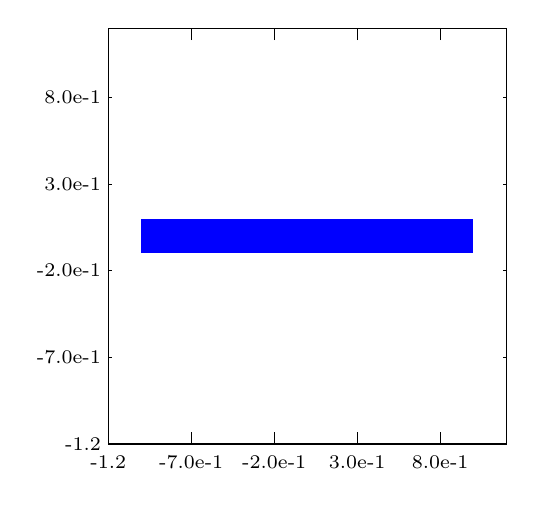
\begin{tikzpicture}[scale = 6,font=\scriptsize]
\draw (0.1148,0.085) rectangle (0.958,0.965);
\foreach \x/\label in {0.1148/-1.2,0.290466/-7.0e-1,0.466133/-2.0e-1,0.6418/3.0e-1,0.817466/8.0e-1} {
  \foreach \y in {0.94,0.085} \draw (\x,\y) -- (\x,\y+0.025);
  \node [below] at (\x,0.08) {\label};
}
\foreach \y/\label in {0.0849996/-1.2,0.268333/-7.0e-1,0.451666/-2.0e-1,0.635/3.0e-1,0.818333/8.0e-1} {
  \foreach \x in {0.951,0.1148} \draw (\x,\y) -- (\x+0.007,\y);
  \node [left] at (0.12,\y) {\label};
}
\fill [blue] (0.185067,0.488333) rectangle (0.887733,0.561667);
\end{tikzpicture}
\hspace{1cm}
% polygon
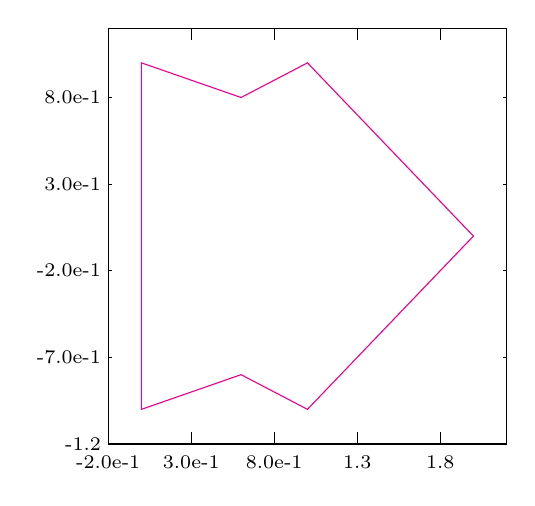
\begin{tikzpicture}[scale = 6,font=\scriptsize]
\draw (0.1148,0.085) rectangle (0.958,0.965);
\foreach \x/\label in {0.1148/-2.0e-1,0.290466/3.0e-1,0.466133/8.0e-1,0.6418/1.3,0.817466/1.8} {
  \foreach \y in {0.94,0.085} \draw (\x,\y) --(\x,\y+0.025);
  \node [below] at (\x,0.08) {\label};
}
\foreach \y/\label in {0.0849996/-1.2,0.268333/-7.0e-1,0.451666/-2.0e-1,0.635/3.0e-1,0.818333/8.0e-1} {
  \foreach \x in {0.951,0.1148} \draw (\x,\y) --(\x+0.007,\y);
  \node [left] at (0.12,\y) {\label};
}
\draw [magenta] (0.185067,0.891667) -- (0.185067,0.158333) -- (0.395867,0.231667) -- (0.5364,0.158333) -- (0.887733,0.525) -- (0.5364,0.891667) -- (0.395867,0.818333) -- cycle;
\end{tikzpicture}
\\[8mm]
% ellipse
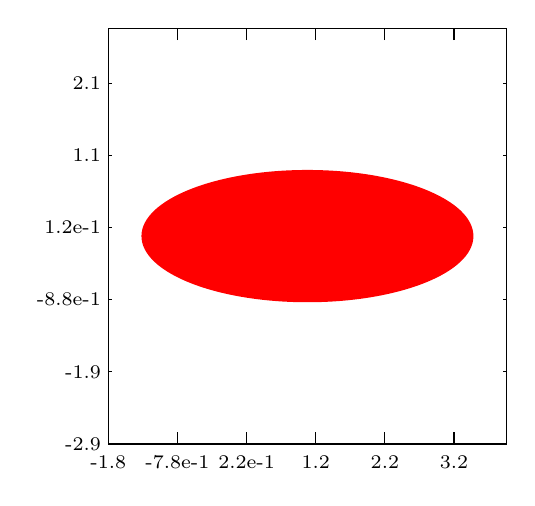
\begin{tikzpicture}[scale = 6,font=\scriptsize]
\draw (0.1148,0.085) rectangle (0.958,0.965);
\foreach \x/\label in {0.1148/-1.8,0.261189/-7.8e-1,0.407578/2.2e-1,0.553966/1.2,0.700355/2.2,0.846744/3.2} {
  \foreach \y in {0.94,0.085} \draw (\x,\y) --(\x,\y+0.025);
  \node [below] at (\x,0.08) {\label};
}
\foreach \y/\label in {0.0849996/-2.9,0.237777/-1.9,0.390555/-8.8e-1,0.543333/1.2e-1,0.696111/1.1,0.848888/2.1} {
  \foreach \x in {0.951,0.1148} \draw (\x,\y) --(\x+0.007,\y);
  \node [left] at (0.12,\y) {\label};
}
\fill [red] (0.5364,0.525) circle [x radius=0.351333,y radius=0.14];
\end{tikzpicture}
\hspace{1cm}
% ring
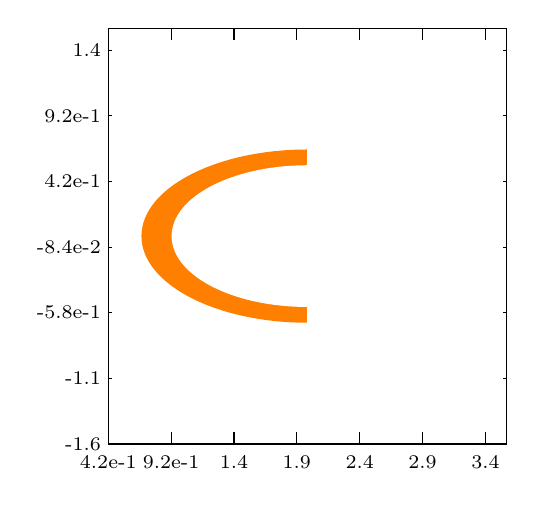
\begin{tikzpicture}[scale = 6,font=\scriptsize]
\draw (0.1148,0.085) rectangle (0.958,0.965);
\foreach \x/\label in {0.1148/4.2e-1,0.247881/9.2e-1,0.380962/1.4,0.514043/1.9,0.647123/2.4,0.780204/2.9,0.913285/3.4} {
  \foreach \y in {0.94,0.085} \draw (\x,\y) --(\x,\y+0.025);
  \node [below] at (\x,0.08) {\label};
}
\foreach \y/\label in {0.0849996/-1.6,0.223888/-1.1,0.362777/-5.8e-1,0.501666/-8.4e-2,0.640555/4.2e-1,0.779444/9.2e-1,0.918333/1.4} {
  \foreach \x in {0.951,0.1148} \draw (\x,\y) --(\x+0.007,\y);
  \node [left] at (0.12,\y) {\label};
}
\fill [color=orange] (0.5364,0.525) circle [x radius=0.351333,y radius=0.183333];
\fill [color=white] (0.5364,0.525) circle [x radius=0.287455,y radius=0.15];
\fill [color=white] (0.5364,0.158333) rectangle (0.9,0.784272);
\end{tikzpicture}
\caption{\label{fig:rg}Sample regions defined via the \ident{RG} class: interval (top left), polygon (top right), ellipse (bottom left), and ring (bottom right). These plots can be generated at run time by adding the command-line option \texttt{-rg\_view draw}.}
\end{figure}

Sometimes it is useful to specify the complement of a certain region, e.g., the part of the complex plane outside an ellipse. This can be achieved with
        \findex{RGSetComplement}
        \begin{Verbatim}[fontsize=\small]
        RGSetComplement(RG rg,PetscBool flg)
        \end{Verbatim}
or in the command line with \Verb!-rg_complement!.

By default, a newly created \ident{RG} object that is not set a type nor parameters must represent the whole complex plane (the same as \texttt{RGINTERVAL} with values $[-\infty,+\infty]\times[-\infty,+\infty]$). We call this the \emph{trivial} region, and provide a function to test this situation:
        \findex{RGIsTrivial}
        \begin{Verbatim}[fontsize=\small]
        RGIsTrivial(RG rg,PetscBool *trivial)
        \end{Verbatim}

Another useful operation is to check whether a given point of the complex plane is inside the region or not:
        \findex{RGCheckInside}
        \begin{Verbatim}[fontsize=\small]
        RGCheckInside(RG rg,PetscInt n,PetscScalar *ar,PetscScalar *ai,PetscInt *inside)
        \end{Verbatim}
Note that the point is represented as two \texttt{PetscScalar}'s, similarly to eigenvalues in \slepc.

\begin{table}
\centering
{\small \begin{tabular}{lll}
                       &                     & {\footnotesize Options} \\
Region Type            & \ident{RGType}      & {\footnotesize Database Name}\\\hline
(Generalized) Interval & \texttt{RGINTERVAL} & \texttt{interval} \\
Polygon                & \texttt{RGPOLYGON}  & \texttt{polygon} \\
Ellipse                & \texttt{RGELLIPSE}  & \texttt{ellipse} \\
Ring                   & \texttt{RGRING}     & \texttt{ring} \\\hline
\end{tabular} }
\caption{\label{tab:rg}Regions available as \ident{RG} objects.}
\end{table}

%---------------------------------------------------
\section{Directory Structure}

The directory structure of the \slepc software is very similar to that in \petsc. The root directory of \slepc contains the following directories:
\begin{description}
\item[\texttt{lib/slepc/conf}] - Directory containing the base \slepc makefile, to be included in application makefiles.
\item[\texttt{config}] - \slepc configuration scripts.
\item[\texttt{docs}] - All documentation for \slepc, including this manual. The subdirectory \texttt{manualpages} contains the on-line manual pages of each \slepc routine.
\item[\texttt{include}] - All include files for \slepc. The following subdirectories exist:
\begin{description}
\setlength{\itemsep}{0mm}
\item[\texttt{slepc/finclude}] - include files for Fortran programmers.
\item[\texttt{slepc/private}] - include files containing implementation details, for developer use only.
\end{description}
\item[\texttt{share/slepc}] - Common files, including:
\begin{description}
\setlength{\itemsep}{0mm}
\item[\texttt{datafiles}] - data files used by some examples.
%\item[\texttt{matlab}] - Matlab interface and examples.
\end{description}
\item[\texttt{src}] - The source code for all \slepc components, which currently includes:
\begin{description}
\setlength{\itemsep}{0mm}
\item[\texttt{sys}] - system-related routines and auxiliary classes \texttt{bv}, \texttt{ds}, \texttt{fn}, \texttt{rg}, \texttt{st}.
\item[\texttt{eps}] - eigenvalue problem solver.
\item[\texttt{svd}] - singular value decomposition solver.
\item[\texttt{pep}] - polynomial eigenvalue problem solver.
\item[\texttt{nep}] - nonlinear eigenvalue problem solver.
\item[\texttt{mfn}] - matrix function.
\item[\texttt{lme}] - linear matrix equations.
\end{description}
\item[\texttt{\$PETSC\_ARCH}] - For each value of \ident{PETSC\_ARCH}, a directory exists containing files generated during installation of that particular configuration. The following subdirectories exist:
\begin{description}
\setlength{\itemsep}{0mm}
\item[\texttt{lib}] - all the generated libraries.
\item[\texttt{lib/slepc/conf}] - configuration parameters and log files.
\item[\texttt{include}] - automatically generated include files, such as Fortran 90 \texttt{*.mod} files.
\end{description}
\end{description}

Each \slepc source code component directory has the following subdirectories:
\begin{description}
\item[\texttt{interface}] - The calling sequences for the abstract interface to the components. Code here does not know about particular implementations.
\item[\texttt{impls}] - Source code for the different implementations.
\item[\texttt{tutorials}] - Example programs intended for learning to use \slepc.
\item[\texttt{tests}] - Example programs used by testing scripts.
\end{description}

%---------------------------------------------------
%\section{Auxiliary Components}
%\label{sec:aux}

%The previous section includes a list of subdirectories, each of them representing a \slepc component. Most of these components have been treated in previous chapters. Here we include a brief report about two auxiliary components, \ident{BV} and \ident{DS}, that are not normally required by final users, but provide important operations to high level solvers such \ident{EPS}.

%\subsection{BV: Basis Vectors}

%\subsection{DS: Direct Solver (or Dense System)}

%---------------------------------------------------
\section{Wrappers to External Libraries}
\label{sec:wrap}

\slepc interfaces to several external libraries for the solution of eigenvalue problems. This section provides a short description of each of these packages as well as some hints for using them with \slepc, including pointers to the respective websites from which the software can be downloaded. The description may also include method-specific parameters, that can be set in the same way as other \slepc options, either procedurally or via the command-line.

In order to use \slepc together with an external library such as \arpack, one needs to do the following.
\begin{enumerate}
\item Install the external software, with the same compilers and MPI that will be used for \petsc/\slepc.
\item Enable the utilization of the external software from \slepc by specifying configure options as explained in \S\ref{sec:opt-inst}.
 \item Build the \slepc libraries.
\item Use the runtime option \Verb!-eps_type <type>! to select the solver.
\end{enumerate}

Exceptions to the above rule are \lapack, which should be enabled during \petsc's configuration, and \blopex, that must be installed with \Verb!--download-blopex! in \slepc's configure. Other packages also support the download option.

\subsection*{\underline{\lapack}}
\begin{description}
\setlength{\itemsep}{0pt}
\item[References.]\citep{Anderson:1999:LUG}.
\item[Website.] \url{https://www.netlib.org/lapack}.
\item[Version.] 3.0 or later.
\item[Summary.] \lapack\ (Linear Algebra PACKage) is a software package for the solution of many different dense linear algebra problems, including various types of eigenvalue problems and singular value decompositions.

\slepc explicitly creates the operator matrix in dense form and then the appropriate \lapack driver routine is invoked. Therefore, this interface should be used only for testing and validation purposes and not in a production code. The operator matrix is created by applying the operator to the columns of the identity matrix.

\item[Installation.]
The \slepc interface to \lapack can be used directly. If \slepc's configure script complains about missing \lapack functions, then configure \petsc with option \texttt{-{}-download-f2cblaslapack}.
\end{description}

\subsection*{\underline{\arpack}}
\begin{description}
\setlength{\itemsep}{0pt}
\item[References.]\citep{Lehoucq:1998:AUG}, \citep{Maschhoff:1996:PEP}.
\item[Website.] \url{https://github.com/opencollab/arpack-ng}.
\item[Version.] Release 2 (plus patches).
\item[Summary.] \arpack\ (ARnoldi PACKage) is a software package for the computation of a few eigenvalues and corresponding eigenvectors of a general $n\times n$ matrix $A$. It is most appropriate for large sparse or structured matrices, where structured means that a matrix-vector product $w \leftarrow Av$ requires order $n$ rather than the usual order $n^2$ floating point operations.

\arpack\ is based upon an algorithmic variant of the Arnoldi process called the Implicitly Restarted Arnoldi Method (IRAM). When the matrix $A$ is symmetric it reduces to a variant of the Lanczos process called the Implicitly Restarted Lanczos Method (IRLM). These variants may be viewed as a synthesis of the Arnoldi/Lanczos process with the Implicitly Shifted QR technique that is suitable for large scale problems.

It can be used for standard and generalized eigenvalue problems, both in real and complex arithmetic. It is implemented in Fortran 77 and it is based on the reverse communication interface. A parallel version, \parpack, is available with support for both MPI and BLACS.
\item[Installation.]
To install from the original website: first of all, unpack \texttt{arpack96.tar.gz} and also the patch file \texttt{patch.tar.gz}. If you plan to use the parallel version, extract also the contents of the file \texttt{parpack96.tar.gz} together with the patches \texttt{ppatch.tar.gz} (make sure you delete any \texttt{mpif.h} files that could exist in the directory tree). After setting all the directories, modify the \texttt{ARmake.inc} file and then compile the software with \texttt{make all}. It is recommended that \arpack is installed with its own \lapack version since it may give unexpected results with more recent versions of \lapack.

Alternatively, one can use the \textsc{arpack-ng} distribution, available in \texttt{github.com}, that supports \texttt{configure}+\texttt{make} for installation. Also, \slepc's \texttt{configure} allows to download this version automatically via the \texttt{-{}-download-arpack} option.

It is possible to configure \slepc with the serial version of \arpack. For this, you have to configure \petsc with the option \texttt{-{}-with-mpi=0}.
\end{description}

\subsection*{\underline{\primme}}
\begin{description}
\setlength{\itemsep}{0pt}
\item[References.]\citep{Stathopoulos:2010:PMS}.
\item[Website.] \url{https://www.cs.wm.edu/~andreas/software}.
\item[Version.] 3.2.
\item[Summary.] \primme (PReconditioned Iterative MultiMethod Eigensolver) is a C library for finding a number of eigenvalues and their corresponding eigenvectors of a real symmetric (or complex Hermitian) matrix. This library provides a multimethod eigensolver, based on Davidson/Jacobi-Davidson. Particular methods include GD+1, JDQMR, and LOBPCG. It supports preconditioning as well as the computation of interior eigenvalues.
\item[Installation.] Type \texttt{make lib} after customizing the file \texttt{Make\_flags} appropriately. Alternatively, the \texttt{-{}-download-primme} option is also available in \slepc's \texttt{configure}.
\item[Specific options.] Since PRIMME contains preconditioned solvers, the \slepc interface uses \ident{STPRECOND}, as described in \ref{sec:precond}.

The \slepc interface to this package allows the user to specify the maximum allowed block size with the function \ident{EPSPRIMMESetBlockSize} or at run time with the option \Verb!-eps_primme_blocksize <size>!.
For changing the particular algorithm within \primme, use the function \ident{EPSPRIMMESetMethod}.

\primme also provides a solver for the singular value decomposition that is interfaced in \slepc's \ident{SVD}, see chapter \ref{cap:svd}.
\end{description}

\subsection*{\underline{\evsl}}
\begin{description}
\setlength{\itemsep}{0pt}
\item[References.]\citep{Li:2019:EVS}.
\item[Website.] \url{https://www-users.cs.umn.edu/~saad/software/EVSL/}.
\item[Summary.] \evsl is a sequential library that implements methods for computing all eigenvalues located in a given interval for real symmetric (standard or generalized) eigenvalue problems. Currently SLEPc only supports standard problems.
\item[Installation.] The option \texttt{-{}-download-evsl} is available in \slepc's configure for easy installation. Alternatively, one can use an already installed version.
\end{description}

\subsection*{\underline{\trlan}}
\begin{description}
\setlength{\itemsep}{0pt}
\item[References.]\citep{Wu:2000:TLM}.
\item[Website.] \url{https://sdm.lbl.gov/\~kewu/trlan.html}.
\item[Version.] 201009.
\item[Summary.] This package provides a Fortran 90 implementation of the dynamic thick-restart Lanczos algorithm. This is a specialized version of Lanczos that targets only the case in which one wants both eigenvalues and eigenvectors of a large real symmetric eigenvalue problem that cannot use the shift-and-invert scheme. In this case the standard non-restarted Lanczos algorithm requires to store a large number of Lanczos vectors, what can cause storage problems and make each iteration of the method very expensive.

\trlan{} requires the user to provide a matrix-vector multiplication routine. The parallel version uses MPI as the message passing layer.
\item[Installation.] To install this package, it is necessary to have access to a Fortran 90 compiler. The compiler name and the options used are specified in the file called \texttt{Make.inc}. To generate the library, type \texttt{make plib} in the \texttt{TRLan} directory. Alternatively, the \texttt{-{}-download-trlan} option is also available in \slepc's \texttt{configure}.

It is possible to configure \slepc with the serial version of \trlan (built with \texttt{make lib}). For this, you have to configure \petsc with the option \texttt{-{}-with-mpi=0}.
\end{description}

\subsection*{\underline{\blopex}}
\begin{description}
\setlength{\itemsep}{0pt}
\item[References.]\citep{Knyazev:2007:BLO}.
\item[Website.] \url{https://github.com/lobpcg/blopex}.
\item[Summary.] \blopex is a package that implements the Locally Optimal Block Preconditioned Conjugate Gradient (LOBPCG) method for computing several extreme eigenpairs of symmetric positive generalized eigenproblems. Numerical comparisons suggest that this method is a genuine analog for eigenproblems of the standard preconditioned conjugate gradient method for symmetric linear systems.
\item[Installation.] In order to use \blopex from \slepc, it necessary to install it during \slepc's configuration: \Verb!./configure --download-blopex!.
\item[Specific options.] Since BLOPEX contains preconditioned solvers, the \slepc interface uses \ident{STPRECOND}, as described in \ref{sec:precond}.
\end{description}

\subsection*{\underline{\scalapack}}
\begin{description}
\setlength{\itemsep}{0pt}
\item[References.]\citep{Blackford:1997:SUG}.
\item[Website.] \url{https://www.netlib.org/scalapack}.
\item[Summary.] \scalapack is a library of high-performance linear algebra routines for parallel distributed memory machines. It contains eigensolvers for dense Hermitian eigenvalue problems, as well as solvers for the (dense) SVD.
\item[Installation.] For using \scalapack from \slepc it is necessary to select it during configuration of \petsc.
\end{description}

\subsection*{\underline{\elpa}}
\begin{description}
\setlength{\itemsep}{0pt}
\item[References.]\citep{Auckenthaler:2011:ELP}.
\item[Website.] \url{https://elpa.mpcdf.mpg.de/}.
\item[Summary.] \elpa is a high-performance library for the parallel solution of dense symmetric (or Hermitian) eigenvalue problems on distributed memory computers. It uses a ScaLAPACK-compatible matrix distribution.
\item[Installation.] The \slepc wrapper to \elpa can be activated at configure time with the option \texttt{-{}-download\_elpa}, in which case \scalapack support must have been enabled during the configuration of \petsc.
\end{description}

\subsection*{\underline{\ksvd}}
\begin{description}
\setlength{\itemsep}{0pt}
\item[References.]\citep{Sukkari:2019:QDW}.
\item[Website.] \url{https://github.com/ecrc/ksvd/}.
\item[Summary.] \ksvd is a high performance software framework for computing a dense SVD on distributed-memory manycore systems. The \ksvd solver relies on the polar decomposition (PD) based on the QR Dynamically-Weighted Halley (QDWH) and ZOLO-PD algorithms.
\item[Installation.] The option \texttt{-{}-download-ksvd} is available in \slepc's configure for easy installation, which in turn requires adding \texttt{-{}-download-polar} and \texttt{-{}-download-elpa}.
\end{description}

\subsection*{\underline{\elemental}}
\begin{description}
\setlength{\itemsep}{0pt}
\item[References.]\citep{Poulson:2013:ELE}.
\item[Website.] \url{https://github.com/elemental/Elemental}.
\item[Summary.] \elemental is distributed-memory, arbitrary-precision, dense and sparse-direct linear algebra package. It contains eigensolvers for dense Hermitian eigenvalue problems, as well as solvers for the SVD.
\item[Installation.] For using \elemental from \slepc it is necessary to select it during configuration of \petsc.
\end{description}

\subsection*{\underline{\feast}}
\begin{description}
\setlength{\itemsep}{0pt}
\item[References.]\citep{Polizzi:2009:DAS}.
\item[Website.] \url{https://feast-solver.org/}.
\item[Summary.] \feast is a numerical library for solving the standard or generalized symmetric eigenvalue problem, and obtaining all the eigenvalues and eigenvectors within a given search interval. It is based on an innovative fast and stable numerical algorithm which deviates fundamentally from the traditional Krylov subspace based iterations or Davidson-Jacobi techniques. The FEAST algorithm takes its inspiration from the density-matrix representation and contour integration technique in quantum mechanics. Latest versions also support non-symmetric problems.
\item[Installation.] We only support the \feast implementation included in Intel MKL. For using it from \slepc it is necessary to configure \petsc with MKL by adding the corresponding option, e.g., \Verb!--with-blas-lapack-dir=$MKLROOT!.
\item[Specific options.] The \slepc interface to \feast allows the user to specify the number of contour integration points with the function \ident{EPSFEASTSetNumPoints} or at run time with the option \Verb!-eps_feast_num_points <n>!.
\end{description}

\subsection*{\underline{\chase}}
\begin{description}
\setlength{\itemsep}{0pt}
\item[References.]\citep{Winkelmann:2019:CCA}.
\item[Website.] \url{https://github.com/ChASE-library/ChASE}.
\item[Summary.] \chase is a modern and scalable library based on subspace iteration with polynomial acceleration to solve dense Hermitian (symmetric) algebraic eigenvalue problems, especially solving dense Hermitian eigenproblems arranged in a sequence. Novel to ChASE is the computation of the spectral estimates that enter in the filter and an optimization of the polynomial degree that further reduces the necessary floating-point operations.
\item[Installation.] Currently, the \chase interface in \slepc is based on the MPI version with block-cyclic distribution, i.e., \scalapack matrix storage, so it is necessary to enable \scalapack during configuration of \petsc.
\end{description}

%---------------------------------------------------
\section{Fortran Interface}
\label{sec:fortran}

\slepc provides an interface for Fortran programmers, very much like \petsc. As in the case of \petsc, there are slight differences between the C and Fortran \slepc interfaces, due to differences in Fortran syntax. For instance, the error checking variable is the final argument of all the routines in the Fortran interface, in contrast to the C convention of providing the error variable as the routine's return value.

The following is a Fortran example. It is the Fortran equivalent of the program given in \S\ref{sec:simpleex} and can be found in \Verb!${SLEPC_DIR}/src/eps/tutorials! (file \texttt{ex1f.F90}).
\MyVerbatimInput{ex1f.F90}

%---------------------------------------------------
%\section{Matlab Interface}
%\label{sec:matlab}
%
%Since version 3.2, \slepc includes an interface intended to make most of \slepc's functionality available from Matlab. It is experimental and needs further development, so users planning to use it seriously are recommended to contact the authors. Below are some guidelines for using this interface.
%
%First of all, \petsc must have been configured with the Matlab interface enabled. This can be done as follows (check \petsc documentation for details):
%       \begin{Verbatim}[fontsize=\small]
%       $ ./configure --with-matlab --with-matlab-engine --with-shared-libraries
%       \end{Verbatim}
%
%Once the \petsc and \slepc libraries have been built, one has to set Matlab's path to point to the directories containing Matlab classes: \Verb!$SLEPC_DIR/share/slepc/matlab/classes! and \Verb!$PETSC_DIR/share/slepc/matlab/classes!. Below we show a simple Matlab example (included in \slepc's distribution) that does this, and then solves a simple eigenproblem.
%\MyVerbatimInput{exEPS.m}



%---------------------------------------------------
\cleardoublepage
\fancyhead{}\fancyhead[LO,RE]{\nouppercase{\scriptsize \sffamily Bibliography}}
\addcontentsline{toc}{chapter}{Bibliography}

%\bibliographystyle{engnat}
%\bibliography{slepc}
%-------------------------------------------------------
% SLEPc Users Manual
%-------------------------------------------------------

\documentclass[titlepage,10pt,a4paper]{book}

\usepackage{xcolor}
\usepackage{graphicx}
\usepackage[square]{natbib}
\usepackage{fancyhdr}
\usepackage{fancyvrb}
\usepackage{caption}
\usepackage{xspace}
\usepackage{ae,aecompl}
\usepackage{amsmath,amssymb}
\usepackage{imakeidx}
\usepackage{hyperref}
\usepackage{titlesec}
\usepackage{tikz,pgfplots}

\makeindex

\hypersetup{
  colorlinks,
  linkcolor=purple,
  citecolor=violet,
  filecolor=blue,
  urlcolor=magenta,
  bookmarksnumbered,
  pdfstartview=FitH,
  pdftitle={SLEPc Users Manual},
  pdfauthor={J. E. Roman, C. Campos, L. Dalcin, E. Romero, A. Tomas},
  pdfsubject={SLEPc: Scalable Library for Eigenvalue Problem Computations},
  pdfkeywords={SLEPc, PETSc, eigenvalue problems}
}

\newcommand{\slepcversion}{3.23}
\newcommand{\slepchome}{https://slepc.upv.es}
\newcommand{\pack}[1]{{\sc #1}\index{\textsc{#1}}\xspace}
\newcommand{\packnoi}[1]{{\sc #1}\xspace}
\newcommand{\slepc}{\texorpdfstring{\packnoi{slep\rm c}}{{SLEPc}}}
\newcommand{\petsc}{\pack{pets\rm c}}
\newcommand{\blas}{\pack{blas}}
\newcommand{\lapack}{\pack{lapack}}
\newcommand{\arpack}{\pack{arpack}}
\newcommand{\parpack}{\pack{parpack}}
\newcommand{\trlan}{\pack{trlan}}
\newcommand{\primme}{\pack{primme}}
\newcommand{\blopex}{\pack{blopex}}
\newcommand{\scalapack}{\pack{scalapack}}
\newcommand{\elpa}{\pack{elpa}}
\newcommand{\elemental}{\pack{elemental}}
\newcommand{\evsl}{\pack{evsl}}
\newcommand{\feast}{\pack{feast}}
\newcommand{\ksvd}{\pack{ksvd}}
\newcommand{\chase}{\pack{chase}}
\newcommand{\mpich}{\pack{mpich}}
\newcommand{\expokit}{\pack{expokit}}
\newcommand{\rutina}[1]{\texttt{#1}\index{\texttt{#1}}}
\newcommand{\ident}[1]{\texttt{#1}\index{\texttt{#1}}}
\newcommand{\findex}[1]{\index{\texttt{#1}}}

\DeclareMathOperator{\rev}{rev}

%VerbatimEnvironment%
\fvset{numbers=left,numbersep=6pt,stepnumber=5}
\newcommand{\MyVerbatimInput}[1]{\fvset{fontsize=\scriptsize}%
  \VerbatimInput{#1}%
  \fvset{fontsize=\normalsize}%
}

\setlength{\textwidth}{14.5cm}
\setlength{\tabcolsep}{2mm}
\renewcommand{\arraystretch}{1.05}
\setcounter{tocdepth}{3}
\renewcommand{\captionlabelfont}{\sl\sffamily}
\makeatletter\@ifundefined{bibfont}{\newcommand{\bibfont}{\small}}{\renewcommand{\bibfont}{\small}}\makeatother

\titleformat{\chapter}[display]
  {\bfseries\Large}
  {\filleft\setlength{\fboxsep}{2mm}\fbox{\large\sc\chaptertitlename}\hspace*{-0.5mm}\setlength{\fboxsep}{4mm}\setlength{\fboxrule}{.5mm}\fbox{\Huge\bfseries\thechapter}}
  {4ex}
  {\huge\bf\sffamily
   \filright}
  [\hfill\rule{10cm}{1pt}]

\begin{document}

\title{
   \vspace*{-1cm}
   \framebox[12cm][l]{
   \includegraphics[height=1.4cm]{figures/upv}
   \hfill
   \parbox[b]{4cm}{\begin{flushright}\vspace*{-7mm}\normalsize\sl\sffamily
   Departamento de\\[-0.8mm] Sistemas Inform\'aticos\\[-0.8mm]
   y Computaci\'on\\[0.8mm]
   \vspace{-2.5mm}\end{flushright}}
   \raisebox{3mm}{\includegraphics[height=9mm,width=1.4cm]{figures/dsic}}
   }
   \\[2cm]
   \normalsize Technical Report DSIC-II/24/02
   \\[2cm]
   \vspace*{6mm}
   {\Large\bf\sffamily
   SLEPc Users Manual\\[2mm]}
   {\large\bf\sffamily
   Scalable Library for Eigenvalue Problem Computations}\\[2mm]
   \vspace*{6mm}
   \vspace*{6mm}
   \url{\slepchome}
   \\[6mm]
}

\author{
  Jose E. Roman\\
  Carmen Campos\\
  Lisandro Dalcin\\
  Eloy Romero\\
  Andr\'es Tom\'as\\[3mm]
}

\date{
   To be used with \slepc \slepcversion\\
   March, 2025
}

\hypersetup{pageanchor=false}
\begin{titlepage}
\maketitle
\end{titlepage}

\setlength{\textheight}{18cm}
\setlength{\oddsidemargin}{0.6cm}
\setlength{\evensidemargin}{0.6cm}
\setlength{\footskip}{2cm}
\setlength{\voffset}{1.3cm}

\pagestyle{empty}
\cleardoublepage
\hypersetup{pageanchor=true}

{
  \pagestyle{plain}
  \pagenumbering{roman}
%---------------------------------------------------
\subsection*{Abstract}

This document describes \slepc, the {\em Scalable Library for Eigenvalue Problem Computations}, a software package for the solution of large sparse eigenproblems on parallel computers. It can be used for the solution of various types of eigenvalue problems, including linear and nonlinear, as well as other related problems such as the singular value decomposition (see a summary of supported problem classes on page \pageref{tab:modules}). \slepc is a general library in the sense that it covers both Hermitian and non-Hermitian problems, with either real or complex arithmetic.

The emphasis of the software is on methods and techniques appropriate for problems in which the associated matrices are large and sparse, for example, those arising after the discretization of partial differential equations. Thus, most of the methods offered by the library are projection methods, including different variants of Krylov and Davidson iterations. In addition to its own solvers, \slepc provides transparent access to some external software packages such as \packnoi{arpack}. These packages are optional and their installation is not required to use \slepc, see \S\ref{sec:wrap} for details. Apart from the solvers, \slepc also provides built-in support for some operations commonly used in the context of eigenvalue computations, such as preconditioning or the shift-and-invert spectral transformation.

\slepc is built on top of \packnoi{pets\rm c}, the Portable, Extensible Toolkit for Scientific Computation \citep{Balay:PUM}. It can be considered an extension of \packnoi{pets\rm c} providing all the functionality necessary for the solution of eigenvalue problems. This means that \packnoi{pets\rm c} must be previously installed in order to use \slepc. \packnoi{pets\rm c} users will find \slepc very easy to use, since it enforces the same programming paradigm. Those readers that are not acquainted with \packnoi{pets\rm c} are highly recommended to familiarize with it before proceeding with \slepc.


\subsubsection*{How to Get \slepc}

All the information related to \slepc can be found at the following web site:
\begin{quote}
\begin{center}
\url{\slepchome}.
\end{center}
\end{quote}
The distribution file is available for download at this site. Other information is provided there, such as installation instructions and contact information. Instructions for installing the software can also be found in \S\ref{sec:inst}.

\packnoi{pets\rm c} can be downloaded from \url{https://petsc.org}.  \packnoi{pets\rm c} is supported, and information on contacting support can be found at that site.

\subsubsection*{Additional Documentation}

This manual provides a general description of \slepc. In addition, manual pages for individual routines are included in the distribution file in hypertext format, and are also available on-line at \url{\slepchome/documentation}. These manual pages provide hyperlinked access to the source code and enable easy movement among related topics. Finally, there are also several hands-on exercises available, which are intended for learning the basic concepts easily.

\subsubsection*{How to Read this Manual}

Users that are already familiar with \packnoi{pets\rm c} can read chapter \ref{cap:int} very fast. Section \ref{sec:eig} provides a brief overview of eigenproblems and the general concepts used by eigensolvers, so it can be skipped by experienced users. Chapters \ref{cap:eps}--\ref{cap:mfn} describe the main \slepc functionality. Some of them include an advanced usage section that can be skipped at a first reading. Finally, chapter \ref{cap:add} contains less important, additional information.

%\subsubsection*{What's New}
%
%The major changes in the Users Manual with respect to the previous version are:
%\begin{itemize}
%\setlength{\itemsep}{-2pt}
%\item New section \S\ref{sec:gsvd} related to the generalized singular value decomposition (GSVD). The rest of Ch.~\ref{cap:svd} has been slightly modified to cover the new GSVD functionality.
%\end{itemize}

\subsubsection*{\slepc Technical Reports}

The information contained in this manual is complemented by a set of Technical Reports, which provide technical details that normal users typically do not need to know but may be useful for experts in order to identify the particular method implemented in \slepc. These reports are not included in the \slepc distribution file but can be accessed via the \slepc web site. A \hyperlink{str}{list of available reports} is included at the end of the Bibliography.


\subsubsection*{Acknowledgments}

%We thank all the \packnoi{pets\rm c} team for their help and support. Without their continued effort invested in \packnoi{pets\rm c}, \slepc would not have been possible.
% We also thank Osni Marques and Tony Drummond for helping us raise awareness of \slepc in the context of the ACTS project.

The current version contains code contributed by:
A.\ Lamas Davi\~{n}a (CUDA code),
F.\ Alvarruiz (restarted Lanczos for the GSVD, structured BSE solvers),
B.\ Mellado-Pinto (structured BSE solvers),
Y.\ Maeda, T.\ Sakurai (CISS solvers),
M.\ Moldaschl, W.\ Gansterer (BDC subroutines),
F.\ Kong (nonlinear inverse iteration),
H.\ Fang, Y. Saad (\textsc{filtlan} polynomial filter).

Development of \slepc has been partially funded by the following grants:
\begin{itemize}
\setlength{\itemsep}{-2pt}
\item Innovation Study ISOLV-BSE has received funding through the Inno4scale project, which is funded by the European High-Performance Computing Joint Undertaking (JU) under Grant Agreement No 101118139. The JU receives support from the European Union's Horizon Europe Programme.
\item Agencia Estatal de Investigaci\'on (Spain), grant no.\ PID2022-139568NB-I00, PI: Jos\'e E. Rom\'an.
\item Agencia Estatal de Investigaci\'on (Spain), grant no.\ PID2019-107379RB-I00, PI: Jos\'e E. Rom\'an.
\item Agencia Estatal de Investigaci\'on (Spain), grant no.\ TIN2016-75985-P, PI: Jos\'e E. Rom\'an.
\item Ministerio de Econom\'{\i}a y Comp.\ (Spain), grant no.\ TIN2013-41049-P, PI: Jos\'e E. Rom\'an.
\item Ministerio de Ciencia e Innovaci\'on (Spain), grant no.\ TIN2009-07519, PI: Jos\'e E. Rom\'an.
\item Valencian Regional Government, grant no.\ GV06/091, PI: Jos\'e E. Rom\'an.
\item Valencian Regional Government, grant no.\ CTIDB/2002/54, PI: Vicente Hern\'andez.
\end{itemize}

\subsubsection*{License and Copyright}

Starting from version 3.8, \slepc is released under a 2-clause BSD license (see \texttt{LICENSE} file).

\begin{quote}
\begin{sffamily}
Copyright 2002--2025 Universitat Polit\`ecnica de Valencia, Spain
\end{sffamily}
\end{quote}

%---------------------------------------------------
\newpage
\subsubsection*{Supported Problem Classes}

The following table provides an overview of the functionality offered by \slepc, organized by problem classes.

\begin{table}[h]
\label{tab:modules}
\centering
{\small \begin{tabular}{lccc}
Problem class                 & Model equation  & Module       & Chapter \\\hline
Linear eigenvalue problem     & $Ax=\lambda x,\quad Ax=\lambda Bx$ & \texttt{EPS} & \ref{cap:eps} \\
Quadratic eigenvalue problem  & $(K+\lambda C+\lambda^2M)x=0$ & -- & -- \\
Polynomial eigenvalue problem & $(A_0+\lambda A_1+\cdots+\lambda^dA_d)x=0$ & \texttt{PEP} & \ref{cap:pep} \\
Nonlinear eigenvalue problem  & $T(\lambda)x=0$ & \texttt{NEP} & \ref{cap:nep} \\\hline
Singular value decomposition  & $Av=\sigma u$   & \texttt{SVD} & \ref{cap:svd} \\
Matrix function (action of)   & $y=f(A)v$   & \texttt{MFN} & \ref{cap:mfn} \\
Linear matrix equation        & $AXE+DXB=C$   & \texttt{LME} & See notes \\\hline
\end{tabular} }
\end{table}

\noindent In order to solve a given problem, one should create a solver object corresponding to the solver class (module) that better fits the problem (the less general one; e.g., we do not recommend using \texttt{NEP} to solve a linear eigenproblem).\\[3mm]

\noindent Notes:\vspace{-2mm}
\begin{itemize}
\setlength{\itemsep}{-2pt}
\item Most users are typically interested in linear eigenproblems only.
\item In each problem class there may exist several subclasses (problem types in \slepc terminology), for instance symmetric-definite generalized eigenproblem in \texttt{EPS}.
\item The solver class (module) is named after the problem class. For historical reasons, the one for linear eigenvalue problems is called \texttt{EPS} rather than \texttt{LEP}.
\item In addition to the SVD shown in the table, the \texttt{SVD} module also supports other related problems such as the GSVD and the HSVD.
\item In previous \slepc versions there was a \texttt{QEP} module for quadratic eigenproblems. It has been replaced by \texttt{PEP}. %See \S\ref{sec:qeppep} for upgrading application code that used \texttt{QEP}.
\item For the action of a matrix function (\texttt{MFN}), in \slepc we focus on methods that are closely related to methods for eigenvalue problems.
\item The solver class \texttt{LME} is still experimental and it is not covered in this manual yet.
\end{itemize}

%---------------------------------------------------
  \setlength{\parskip}{0cm}
  \tableofcontents
}
\cleardoublepage
\pagenumbering{arabic}
\pagestyle{fancy}
\renewcommand{\chaptermark}[1]{\markboth{\scriptsize \sffamily {\bfseries\chaptername\ \thechapter.} #1}{}}
\renewcommand{\sectionmark}[1]{\markright{\scriptsize \sffamily {\bfseries\thesection.} #1}{}}
\fancyhead{}
\fancyhead[LE,RO]{\nouppercase{\rightmark}}
\fancyhead[LO,RE]{\nouppercase{\leftmark}}
\fancyfoot[C]{\scriptsize --- \thepage\ ---}
\renewcommand{\headrulewidth}{0.2pt}
\renewcommand{\footrulewidth}{0.2pt}

\include{intro}
\include{eps}
\include{st}
\include{svd}
\include{pep}
\include{nep}
\include{mfn}
\include{extra}

%---------------------------------------------------
\cleardoublepage
\fancyhead{}\fancyhead[LO,RE]{\nouppercase{\scriptsize \sffamily Bibliography}}
\addcontentsline{toc}{chapter}{Bibliography}

%\bibliographystyle{engnat}
%\bibliography{slepc}
\input{slepc.bbl}

{\bibfont
\paragraph{SLEPc Technical Reports}
\hypertarget{str}{}
(Note: these reports are available through the \href{https://slepc.upv.es}{\slepc web site}.)
\begin{list}{}{\setlength{\labelwidth}{3cm}\setlength{\leftmargin}{12.5mm}}
\item[\textrm{\sffamily[STR-1]}] V. Hern\'andez, J. E. Rom\'an, A. Tom\'as, V. Vidal. ``Orthogonalization Routines in \slepc.''
\item[\textrm{\sffamily[STR-2]}] V. Hern\'andez, J. E. Rom\'an, A. Tom\'as, V. Vidal. ``Single Vector Iteration Methods in \slepc.''
\item[\textrm{\sffamily[STR-3]}] V. Hern\'andez, J. E. Rom\'an, A. Tom\'as, V. Vidal. ``Subspace Iteration in \slepc.''
\item[\textrm{\sffamily[STR-4]}] V. Hern\'andez, J. E. Rom\'an, A. Tom\'as, V. Vidal. ``Arnoldi Methods in \slepc.''
\item[\textrm{\sffamily[STR-5]}] V. Hern\'andez, J. E. Rom\'an, A. Tom\'as, V. Vidal. ``Lanczos Methods in \slepc.''
\item[\textrm{\sffamily[STR-6]}] V. Hern\'andez, J. E. Rom\'an, A. Tom\'as, V. Vidal. ``A Survey of Software for Sparse Eigenvalue Problems.''
\item[\textrm{\sffamily[STR-7]}] V. Hern\'andez, J. E. Rom\'an, A. Tom\'as, V. Vidal. ``Krylov-Schur Methods in \slepc.''
\item[\textrm{\sffamily[STR-8]}] V. Hern\'andez, J. E. Rom\'an, A. Tom\'as. ``Restarted Lanczos Bidiagonalization for the SVD in \slepc.''
\item[\textrm{\sffamily[STR-9]}] J. E. Rom\'an. ``Practical Implementation of Harmonic Krylov-Schur.''
\item[\textrm{\sffamily[STR-10]}] M. E. Hochstenbach, E. Romero, J. E. Roman. ``Davidson Type Subspace Expansions for the Linear Eigenvalue Problem.''
\item[\textrm{\sffamily[STR-11]}] Y. Maeda, T. Sakurai, J. E. Roman. ``Contour Integral Spectrum Slicing Method in \slepc.''
\end{list}
}

\cleardoublepage
\fancyhead{}\fancyhead[LO,RE]{\nouppercase{\scriptsize \sffamily Index}}
\addcontentsline{toc}{chapter}{Index}
\printindex
\cleardoublepage

\end{document}



{\bibfont
\paragraph{SLEPc Technical Reports}
\hypertarget{str}{}
(Note: these reports are available through the \href{https://slepc.upv.es}{\slepc web site}.)
\begin{list}{}{\setlength{\labelwidth}{3cm}\setlength{\leftmargin}{12.5mm}}
\item[\textrm{\sffamily[STR-1]}] V. Hern\'andez, J. E. Rom\'an, A. Tom\'as, V. Vidal. ``Orthogonalization Routines in \slepc.''
\item[\textrm{\sffamily[STR-2]}] V. Hern\'andez, J. E. Rom\'an, A. Tom\'as, V. Vidal. ``Single Vector Iteration Methods in \slepc.''
\item[\textrm{\sffamily[STR-3]}] V. Hern\'andez, J. E. Rom\'an, A. Tom\'as, V. Vidal. ``Subspace Iteration in \slepc.''
\item[\textrm{\sffamily[STR-4]}] V. Hern\'andez, J. E. Rom\'an, A. Tom\'as, V. Vidal. ``Arnoldi Methods in \slepc.''
\item[\textrm{\sffamily[STR-5]}] V. Hern\'andez, J. E. Rom\'an, A. Tom\'as, V. Vidal. ``Lanczos Methods in \slepc.''
\item[\textrm{\sffamily[STR-6]}] V. Hern\'andez, J. E. Rom\'an, A. Tom\'as, V. Vidal. ``A Survey of Software for Sparse Eigenvalue Problems.''
\item[\textrm{\sffamily[STR-7]}] V. Hern\'andez, J. E. Rom\'an, A. Tom\'as, V. Vidal. ``Krylov-Schur Methods in \slepc.''
\item[\textrm{\sffamily[STR-8]}] V. Hern\'andez, J. E. Rom\'an, A. Tom\'as. ``Restarted Lanczos Bidiagonalization for the SVD in \slepc.''
\item[\textrm{\sffamily[STR-9]}] J. E. Rom\'an. ``Practical Implementation of Harmonic Krylov-Schur.''
\item[\textrm{\sffamily[STR-10]}] M. E. Hochstenbach, E. Romero, J. E. Roman. ``Davidson Type Subspace Expansions for the Linear Eigenvalue Problem.''
\item[\textrm{\sffamily[STR-11]}] Y. Maeda, T. Sakurai, J. E. Roman. ``Contour Integral Spectrum Slicing Method in \slepc.''
\end{list}
}

\cleardoublepage
\fancyhead{}\fancyhead[LO,RE]{\nouppercase{\scriptsize \sffamily Index}}
\addcontentsline{toc}{chapter}{Index}
\printindex
\cleardoublepage

\end{document}



{\bibfont
\paragraph{SLEPc Technical Reports}
\hypertarget{str}{}
(Note: these reports are available through the \href{https://slepc.upv.es}{\slepc web site}.)
\begin{list}{}{\setlength{\labelwidth}{3cm}\setlength{\leftmargin}{12.5mm}}
\item[\textrm{\sffamily[STR-1]}] V. Hern\'andez, J. E. Rom\'an, A. Tom\'as, V. Vidal. ``Orthogonalization Routines in \slepc.''
\item[\textrm{\sffamily[STR-2]}] V. Hern\'andez, J. E. Rom\'an, A. Tom\'as, V. Vidal. ``Single Vector Iteration Methods in \slepc.''
\item[\textrm{\sffamily[STR-3]}] V. Hern\'andez, J. E. Rom\'an, A. Tom\'as, V. Vidal. ``Subspace Iteration in \slepc.''
\item[\textrm{\sffamily[STR-4]}] V. Hern\'andez, J. E. Rom\'an, A. Tom\'as, V. Vidal. ``Arnoldi Methods in \slepc.''
\item[\textrm{\sffamily[STR-5]}] V. Hern\'andez, J. E. Rom\'an, A. Tom\'as, V. Vidal. ``Lanczos Methods in \slepc.''
\item[\textrm{\sffamily[STR-6]}] V. Hern\'andez, J. E. Rom\'an, A. Tom\'as, V. Vidal. ``A Survey of Software for Sparse Eigenvalue Problems.''
\item[\textrm{\sffamily[STR-7]}] V. Hern\'andez, J. E. Rom\'an, A. Tom\'as, V. Vidal. ``Krylov-Schur Methods in \slepc.''
\item[\textrm{\sffamily[STR-8]}] V. Hern\'andez, J. E. Rom\'an, A. Tom\'as. ``Restarted Lanczos Bidiagonalization for the SVD in \slepc.''
\item[\textrm{\sffamily[STR-9]}] J. E. Rom\'an. ``Practical Implementation of Harmonic Krylov-Schur.''
\item[\textrm{\sffamily[STR-10]}] M. E. Hochstenbach, E. Romero, J. E. Roman. ``Davidson Type Subspace Expansions for the Linear Eigenvalue Problem.''
\item[\textrm{\sffamily[STR-11]}] Y. Maeda, T. Sakurai, J. E. Roman. ``Contour Integral Spectrum Slicing Method in \slepc.''
\end{list}
}

\cleardoublepage
\fancyhead{}\fancyhead[LO,RE]{\nouppercase{\scriptsize \sffamily Index}}
\addcontentsline{toc}{chapter}{Index}
\printindex
\cleardoublepage

\end{document}



{\bibfont
\paragraph{SLEPc Technical Reports}
\hypertarget{str}{}
(Note: these reports are available through the \href{https://slepc.upv.es}{\slepc web site}.)
\begin{list}{}{\setlength{\labelwidth}{3cm}\setlength{\leftmargin}{12.5mm}}
\item[\textrm{\sffamily[STR-1]}] V. Hern\'andez, J. E. Rom\'an, A. Tom\'as, V. Vidal. ``Orthogonalization Routines in \slepc.''
\item[\textrm{\sffamily[STR-2]}] V. Hern\'andez, J. E. Rom\'an, A. Tom\'as, V. Vidal. ``Single Vector Iteration Methods in \slepc.''
\item[\textrm{\sffamily[STR-3]}] V. Hern\'andez, J. E. Rom\'an, A. Tom\'as, V. Vidal. ``Subspace Iteration in \slepc.''
\item[\textrm{\sffamily[STR-4]}] V. Hern\'andez, J. E. Rom\'an, A. Tom\'as, V. Vidal. ``Arnoldi Methods in \slepc.''
\item[\textrm{\sffamily[STR-5]}] V. Hern\'andez, J. E. Rom\'an, A. Tom\'as, V. Vidal. ``Lanczos Methods in \slepc.''
\item[\textrm{\sffamily[STR-6]}] V. Hern\'andez, J. E. Rom\'an, A. Tom\'as, V. Vidal. ``A Survey of Software for Sparse Eigenvalue Problems.''
\item[\textrm{\sffamily[STR-7]}] V. Hern\'andez, J. E. Rom\'an, A. Tom\'as, V. Vidal. ``Krylov-Schur Methods in \slepc.''
\item[\textrm{\sffamily[STR-8]}] V. Hern\'andez, J. E. Rom\'an, A. Tom\'as. ``Restarted Lanczos Bidiagonalization for the SVD in \slepc.''
\item[\textrm{\sffamily[STR-9]}] J. E. Rom\'an. ``Practical Implementation of Harmonic Krylov-Schur.''
\item[\textrm{\sffamily[STR-10]}] M. E. Hochstenbach, E. Romero, J. E. Roman. ``Davidson Type Subspace Expansions for the Linear Eigenvalue Problem.''
\item[\textrm{\sffamily[STR-11]}] Y. Maeda, T. Sakurai, J. E. Roman. ``Contour Integral Spectrum Slicing Method in \slepc.''
\end{list}
}

\cleardoublepage
\fancyhead{}\fancyhead[LO,RE]{\nouppercase{\scriptsize \sffamily Index}}
\addcontentsline{toc}{chapter}{Index}
\printindex
\cleardoublepage

\end{document}

